%%%%%%%%%%%%%%%%%%%%%%%%%%%%%%%%%%%%%%%%%
% SUTD Masters/Doctoral Thesis
% LaTeX Template
% Version 1.0 (29/08/16)
%
% Adapted to SUTD requirements by Martin Ochoa
%
% This template is based on a template downloaded from:
% http://www.LaTeXTemplates.com
%
% Version 2.x major modifications by:
% Vel (vel@latextemplates.com)
%
% which in turn was based on a template by:
% Steve Gunn (http://users.ecs.soton.ac.uk/srg/softwaretools/document/templates/)
% Sunil Patel (http://www.sunilpatel.co.uk/thesis-template/)
%
%
% Template license:
% CC BY-NC-SA 3.0 (http://creativecommons.org/licenses/by-nc-sa/3.0/)
%
%%%%%%%%%%%%%%%%%%%%%%%%%%%%%%%%%%%%%%%%%

%----------------------------------------------------------------------------------------
%	PACKAGES AND OTHER DOCUMENT CONFIGURATIONS
%----------------------------------------------------------------------------------------

\documentclass[
11pt, % The default document font size, options: 10pt, 11pt, 12pt
oneside, % Two side (alternating margins) for binding by default, uncomment to switch to one side
english, % ngerman for German
onehalfspacing, % Single line spacing, alternatives: onehalfspacing or doublespacing
%draft, % Uncomment to enable draft mode (no pictures, no links, overfull hboxes indicated)
%nolistspacing, % If the document is onehalfspacing or doublespacing, uncomment this to set spacing in lists to single
%liststotoc, % Uncomment to add the list of figures/tables/etc to the table of contents
%toctotoc, % Uncomment to add the main table of contents to the table of contents
%parskip, % Uncomment to add space between paragraphs
%nohyperref, % Uncomment to not load the hyperref package
headsepline, % Uncomment to get a line under the header
]{MastersDoctoralThesis} % The class file specifying the document structure

\usepackage[utf8]{inputenc} % Required for inputting international characters
\usepackage[T1]{fontenc} % Output font encoding for international characters

\usepackage{array} % table formatting

\usepackage{palatino} % Use the Palatino font by default
\usepackage[style=authoryear,natbib=true]{biblatex} % User the bibtex backend with the authoryear citation style (which resembles APA)

\addbibresource{thesis.bib} % The filename of the bibliography
\usepackage[autostyle=true]{csquotes} % Required to generate language-dependent quotes in the bibliography

\hypersetup{%
  colorlinks = true,
  linkcolor  = black
}

%----------------------------------------------------------------------------------------
%	MARGIN SETTINGS
%----------------------------------------------------------------------------------------

\geometry{
	paper=a4paper, % Change to letterpaper for US letter
	inner=2.54cm, % Inner margin
	outer=2.8cm, % Outer margin
	bindingoffset=1cm, % Binding offset
	top=2.5cm, % Top margin
	bottom=2.5cm, % Bottom margin
	%showframe,% show how the type block is set on the page
}

%----------------------------------------------------------------------------------------
%	THESIS INFORMATION
%----------------------------------------------------------------------------------------

\thesistitle{Quantifying the Value of Information and Collaboration in the Decentralized ASEAN Airspace Network} % Your thesis title, this is used in the title and abstract, print it elsewhere with \ttitle
\supervisor{Dr. Nuno \textsc{Ribeiro}} % Your supervisor's name, this is used in the title page, print it elsewhere with \supname
\examiner{} % Your examiner's name, this is not currently used anywhere in the template, print it elsewhere with \examname
\degree{Doctor of Philosophy} % Your degree name, this is used in the title page and abstract, print it elsewhere with \degreename
\author{Darryl \textsc{Teo}} % Your name, this is used in the title page and abstract, print it elsewhere with \authorname
\addresses{} % Your address, this is not currently used anywhere in the template, print it elsewhere with \addressname
\university	{SUTD}
\keywords{} % Keywords for your thesis, this is not currently used anywhere in the template, print it elsewhere with \keywordnames
\pillar{Engineering Systems and Design} % Pillar

\hypersetup{pdftitle=\ttitle} % Set the PDF's title to your title
\hypersetup{pdfauthor=\authorname} % Set the PDF's author to your name
\hypersetup{pdfkeywords=\keywordnames} % Set the PDF's keywords to your keywords

\begin{document}

\frontmatter % Use roman page numbering style (i, ii, iii, iv...) for the pre-content pages

\pagestyle{plain} % Default to the plain heading style until the thesis style is called for the body content

%----------------------------------------------------------------------------------------
%	TITLE PAGE
%----------------------------------------------------------------------------------------

\begin{titlepage}
\begin{center}

\begin{figure}
\centering
\includegraphics[width=0.5\textwidth]{Figures/SUTD.pdf}
\end{figure}

\hfill\break\\[1.5cm]

{\huge \bfseries \ttitle}\\[3cm] % Thesis title


Submitted by\\[0.5cm]
\authorname % Author name - remove the \href bracket to remove the link

\vspace{3em}

Thesis Advisor\\[0.5cm]
\supname % Supervisor name - remove the \href bracket to remove the link
\\Assistant Professor, Engineering Systems and Design
\\Deputy Director, Aviation Studies Institute

\vspace{3em}

\pillarname\\[1cm] % Research group name and department name

\large{A thesis submitted to the Singapore University of Technology and Design in fulfillment of the requirement for the degree of \degreename}\\[1cm] % University requirement text


{\large \the\year}\\[2cm] % Date
%\includegraphics{Logo} % University/department logo - uncomment to place it

\vfill
\end{center}
\end{titlepage}

%----------------------------------------------------------------------------------------
%	DECLARATION PAGE
%----------------------------------------------------------------------------------------

\begin{tec}
\addchaptertocentry{\tecname}
\begin{tabular}{ll}
	TEC Chair: & \underline{Karthik Natarajan} \\
 	& Professor \\
	& --- Pillar of Engineering Systems and Design \vspace{2em}\\

        Main Advisor: & \underline{Nuno Ribeiro} \\
	& Assistant Professor \\
	& --- Pillar of Engineering Systems and Design \\
        & Deputy Director \\
	& --- Aviation Studies Institute \vspace{2em}\\

	Co-Advisor: & \underline{Peter Jackson} \\
	& Professor and Former Head of Pillar \\
	& --- Pillar of Engineering Systems and Design \\
	& Distinguished Visiting Professor \\
	& --- Aviation Studies Institute \vspace{2em}\\
	
	Internal TEC member 1: & \underline{Antonios Varvitsiotis} \\
	& Assistant Professor \\
	& --- Pillar of Engineering Systems and Design \vspace{2em}\\
	
        Internal TEC member 2: & \underline{Karthyek Murthy} \\
	& Assistant Professor \\
	& --- Pillar of Engineering Systems and Design \vspace{2em}\\
\end{tabular}
\end{tec}
\vfill\eject

%----------------------------------------------------------------------------------------
%	DECLARATION PAGE
%----------------------------------------------------------------------------------------

% \begin{declaration}
% \addchaptertocentry{\authorshipname}

% \noindent I, \authorname, declare that this thesis titled, \enquote{\ttitle} and the work presented in it are my own. I confirm that:
%
% \begin{itemize}
% \item This work was done wholly or mainly while in candidature for a research degree at this University.
% \item Where any part of this thesis has previously been submitted for a degree or any other qualification at this University or any other institution, this has been clearly stated.
% \item Where I have consulted the published work of others, this is always clearly attributed.
% \item Where I have quoted from the work of others, the source is always given. With the exception of such quotations, this thesis is entirely my own work.
% \item I have acknowledged all main sources of help.
% \item Where the thesis is based on work done by myself jointly with others, I have made clear exactly what was done by others and what I have contributed myself.\\
% \end{itemize}

% I hereby confirm the following:
% \begin{itemize}
% \item I hereby confirm that the thesis work is original and has not been submitted to any other University or Institution for higher degree purposes.
% \item I hereby grant SUTD the permission to reproduce and distribute publicly paper and electronic copies of this thesis document in whole or in part in any medium now known or hereafter created in accordance with Policy on Intellectual Property, clause 4.2.2.
% \item I have fulfilled all requirements as prescribed by the University and provided 1 copy of my thesis in PDF.
% \item I have attached all publications and award list related to the thesis (e.g. journal, conference report and patent).
% \item The thesis does / does not (delete accordingly) contain patentable or confidential information.
% \item I certify that the thesis has been checked for plagiarism via turnitin/ithenticate. The score is 100\%.
% \end{itemize}

% \noindent Name and signature:\\
% \rule[0.5em]{25em}{0.5pt} % This prints a line for the signature

% \noindent Date:\\
% \rule[0.5em]{25em}{0.5pt} % This prints a line to write the date
% \end{declaration}

% \cleardoublepage

%----------------------------------------------------------------------------------------
%	QUOTATION PAGE
%----------------------------------------------------------------------------------------

% Uncomment for quotation page
% \vspace*{0.2\textheight}
%
% \noindent\enquote{\itshape Thanks to my solid academic training, today I can write hundreds of words on virtually any topic without possessing a shred of information, which is how I got a good job in journalism.}\bigbreak
%
% \hfill Dave Barry

%----------------------------------------------------------------------------------------
%	ABSTRACT PAGE
%----------------------------------------------------------------------------------------

\begin{abstract}
\addchaptertocentry{\abstractname} % Add the abstract to the table of contents
\textit{Reimagining Air Traffic Flow Management (ATFM) --- toward a smarter, more resilient future}. While information sharing and collaborative decision-making are well-established in regions such as the United States and Europe, Southeast Asia continues to operate in a highly decentralized manner, posing significant challenges to the effective implementation of ATFM. A major undertaking to support a transition into a collaborative environment is the Flight \& Flow Information for a Collaborative Environment (FF-ICE) initiative, conceived to eliminate the limitations of the current Flight Plan system.

This dissertation presents the first comprehensive quantitative study of the FF-ICE program, examining the benefits and drawbacks of an incremental FF-ICE R1 implementation in the ASEAN region. Owing to the interconnectivity, complexity, uncertainty, and decentralized nature of the ASEAN airspace, solving the ATFM problem at the scale of the entire region fails to capture the operational nuances, particularly because incremental participation is anticipated. To address this, we introduce a Rolling Horizon Concept (RHC) that more accurately represents varying levels of information sharing and aligns more closely with current operational capabilities.

We present a suite of mathematical models and algorithmic routines designed to simulate decentralized ATFM systems, incorporating key constraints such as airspace capacity and aircraft separation requirements. These algorithms operate independently within each region, using the available information at each time step to optimize ATFM decisions including speed adjustments, ground delay programs and airborne holding.

A realistic simulator of the ASEAN airspace network, supporting information sharing and collaborative decision-making, was developed using the proposed mathematical tools and real airspace data. The results demonstrate significant savings under various collaboration regimes. Notably, partial collaboration, even within a single country, can yield considerable benefits. The results also reveal a surprising consequence of minor collaborations, say between only two airports, that has been shown to erratically impact other flights far from the time which collaborative measures take place.

\end{abstract}

%----------------------------------------------------------------------------------------
%	Publications
%----------------------------------------------------------------------------------------

\begin{publications}
\addchaptertocentry{\publicationsname} % Add the abstract to the table of contents
Darryl Teo, Peter Jackson, Daniel Delahaye, and Nuno Ribeiro. "Optimization-Based Simulation of Air Traffic Flow Management Within the Decentralized ASEAN Region" In: \textit{Computers \& Operations Research (Major Revision). Preprint available at: \href{https://papers.ssrn.com/sol3/papers.cfm?abstract_id=5173282}{ssrn}}. Supporting paper for Chapters \ref{chap4} and \ref{chap5}.

Darryl Teo, Peter Jackson, Nuno Ribeiro, Rakesh Nandi, and Gengling Dai. "Estimating the Benefits of Information Sharing and Collaboration in a Decentralized Flight Network" In: \textit{Working paper}. Supporting paper for Chapters \ref{chap6} and \ref{chap7}.
\end{publications}

\begin{presentations}
    \addchaptertocentry{\presentationsname} % Add the abstract to the table of contents
    Darryl Teo, Peter Jackson, and Daniel Delahaye. "Measuring the Value of Ground Delay Programs in the ASEAN Airspace" In: \textit{Presentation at the Singapore Aviation Research Technology Exchange Day (2025)}
    
    Darryl Teo, Peter Jackson, Nuno Ribeiro, Gengling Dai, and Rakesh Nandi. "Quantifying Airspace Network Benefits and Impacts on Non-Participating Flights Under the FF-ICE R1 Initiative" In: \textit{Presentation at the 2025 INFORMS International Meeting (2025)}

    Darryl Teo, Peter Jackson, Nuno Ribeiro, Gengling Dai, and Rakesh Nandi. "Simulated Impact of the FF-ICE R1 Initiative Under Multiple Capacity Constraints and Collaboration" In: \textit{Presentation at the 28th ATRS World Conference (2025)}
    
    Darryl Teo, Peter Jackson, and Daniel Delahaye. "Optimization Algorithms Applied to the ASEAN Airspace" In: \textit{Presentation at the NUS SG Analytics and Operations Day 2024 (2024)}
    
    Darryl Teo, Peter Jackson, Nuno Ribeiro, Gengling Dai, and Rakesh Nandi. "Simulated Impact of the FF-ICE R1 Initiative With Incremental Participation" In: \textit{Presentation at the INFORMS 2024 Annual Meeting (2024)}
    
\end{presentations}

%----------------------------------------------------------------------------------------
%	ACKNOWLEDGEMENTS
%----------------------------------------------------------------------------------------

\begin{acknowledgements}
\addchaptertocentry{\acknowledgementname} % Add the acknowledgements to the table of contents

First and foremost, I would like to thank Prof PJ for believing in me, and giving me this amazing opportunity to pursue the PhD. To Prof PJ: From day one until now, I could not have asked for a better mentor, who exhibits the values of care, integrity, industriousness, friendliness and beyond. The way you treat everyone with respect, regardless of social status, has left a deep impression on me, and I strive to follow in your footsteps. Also, no matter how busy you were, you always found time to respond and help me with my tasks or personal matters, and I am extremely grateful for your generosity with time. I have grown so much in the past few years thanks to your mentorship, developing as a better researcher, as well as a better human, and I endeavor to emulate your example! Wishing you and your family good health and happiness.

Next, I would like to thank Prof Nuno for advising my PhD for the past two years, and always offering advice and help whenever I needed it. I thank you for the knowledge you have imparted, and guidance you have generously offered over the many years we have known each other. To Prof Nuno: I am continually impressed by your ability to analyze data and offer insights that few others can. Your ability to create convincing arguments is truly admirable. I am deeply grateful to have learned from you --— your mentorship has greatly boosted my confidence in presenting and articulating my ideas. Furthermore, during our conversations, I feel as if I am talking to another Singaporean; your ability and adapt and thrive in new surroundings is a powerful and enviable trait. The stories of your adventures overseas have never failed to captivate me and opened my eyes to how big the world is. Thank you so much for your guidance and I look forward to future collaborations together.

I would like to thank Prof Daniel for hosting me at Ecole Nationale de l'Aviation Civile. To Prof Daniel: Thank you for taking care of me during my stay in Toulouse, France, and beyond. It was my first time living abroad, and while scary at first, my fears dissipated soon after, in no small part due to your warmth and kindness. Your vast knowledge on aviation and reputation in the field has left me starstruck, and I am proud to have you as my mentor. In addition, your physical ability is extremely impressive --- the intensity of your cycles and mountain climbing, and frequent travels, has become a tale of legends in my book. Thank you for dropping by whenever you visit Singapore too, I am always happy to see you again. Wishing you good health, and safe travels! Merci beaucoup!

I also wish to express my heartfelt gratitude to Chen Sin Chee, for being the best graduate studies manager. He has always gone above and beyond to help me whenever I face any difficulty in any administrative or personal matters. Thank you to Prof Jeffery Chan for the interesting discussions during the ethics class, and encouraging me to enroll into the PhD program. Thank you to Cecilia Radhalechumi, Samantha Septribellina, Lim Lee Chen, and Tan Siew Gan for always helping to schedule meetings and other admin matters; there has been 0 hiccups as far as I recall, amazing! Thank you to Prof Bikramjit Das and Prof Stefano Galelli for providing guidance during my term as your teaching assistant. Thank you to Li Hongbo and Ruan Yanqiu for the teamwork and support as friends and groupmates during the PhD coursework. Thank you to my project mates over the past few years --- Gengling Dai, Rakesh Nandi, Wang Weimeng, Ho Huiqi, Chua Wanyun, Faye Chiang; you have been the most amazing people to work with. Thank you to everyone in the ESD office for the welcoming environment, especially during my undergrad days. Thank you to everyone in the ASI office for making it an enjoyable place to work. Thank you to the PhD matters office for the smooth processing of all the overseas attachments and conferences I have attended. I would like to extend my sincere thanks to everyone I had the pleasure of interacting with during my time at SUTD. My experience has left me with a lasting impression of SUTD as a highly efficient research institution that offers world-class education and is home to exceptionally capable and welcoming staff and students.

I would also like to thank SUTD for the generous funding provided under the PGF(CIS) scholarship, and CAAS for funding many projects within the ASI.

Last but not least, I would like to thank God, and my family. I thank the Lord for blessing me with this opportunity, and keeping me from harm; I will seek your ways in all seasons of life. \textit{The heart of man plans his way, but the LORD establishes his steps. -Proverbs 16:9}. To my family: Home is where the heart is, and my heart lies with you. Thank you for being there for me, supporting and encouraging me always; the love and warmth of our family is irreplaceable.  My mother's favorite quote: "A watermelon in a box will end up square.". Given that the shape of a watermelon is determined by its surroundings, I hope to pursue the next chapter of my life in an environment that positively shapes my personal and professional life and do you proud.

\end{acknowledgements}

%----------------------------------------------------------------------------------------
%	LIST OF CONTENTS/FIGURES/TABLES PAGES
%----------------------------------------------------------------------------------------

\tableofcontents % Prints the main table of contents

\listoffigures % Prints the list of figures

\listoftables % Prints the list of tables

\listofalgorithms % Prints the list of algorithms

%----------------------------------------------------------------------------------------
%	ABBREVIATIONS
%----------------------------------------------------------------------------------------

% Uncomment for abbreviations page
% \begin{abbreviations}{ll} % Include a list of abbreviations (a table of two columns)
%
% \textbf{LAH} & \textbf{L}ist \textbf{A}bbreviations \textbf{H}ere\\
% \textbf{WSF} & \textbf{W}hat (it) \textbf{S}tands \textbf{F}or\\
%
% \end{abbreviations}

%----------------------------------------------------------------------------------------
%	PHYSICAL CONSTANTS/OTHER DEFINITIONS
%----------------------------------------------------------------------------------------

% Uncomment for physical constants etc
% \begin{constants}{lr@{${}={}$}l} % The list of physical constants is a three column table
%
% % The \SI{}{} command is provided by the siunitx package, see its documentation for instructions on how to use it
%
% 	Speed of Light & $c_{0}$ & \SI{2.99792458e8}{\meter\per\second} (exact)\\
% %Constant Name & $Symbol$ & $Constant Value$ with units\\
%
% \end{constants}

%----------------------------------------------------------------------------------------
%	SYMBOLS
%----------------------------------------------------------------------------------------

% Uncomment for symbols
% \begin{symbols}{lll} % Include a list of Symbols (a three column table)
%
% $a$ & distance & \si{\meter} \\
% $P$ & power & \si{\watt} (\si{\joule\per\second}) \\
% %Symbol & Name & Unit \\
%
% \addlinespace % Gap to separate the Roman symbols from the Greek
%
% $\omega$ & angular frequency & \si{\radian} \\
%
% \end{symbols}

%----------------------------------------------------------------------------------------
%	DEDICATION
%----------------------------------------------------------------------------------------

% \dedicatory{For/Dedicated to/To my\ldots}

%----------------------------------------------------------------------------------------
%	THESIS CONTENT - CHAPTERS
%----------------------------------------------------------------------------------------

\mainmatter % Begin numeric (1,2,3...) page numbering

\pagestyle{thesis} % Return the page headers back to the "thesis" style

% Include the chapters of the thesis as separate files from the Chapters folder
% Uncomment the lines as you write the chapters

\chapter{Introduction}
\label{chap1}
As our world becomes increasingly globalized, international travel, trade, and other business activities have continued to fuel growth in the extensive industry that is aviation. For a sense of scale, the aviation sectors' contribution as a percent of GDP, including tourism, ranges from 3.2$\%$ of Canada's GDP, to 11.8$\%$ of Singapore's GDP, and for a more extreme example, 58.8$\%$ of Maldive's GDP \parencite{IATA2020}. 

Despite the meltdown in aviation services during the COVID-19 pandemic, the recovery has been strong, with flight revenues at the end of 2023 exceeding pre-pandemic levels by seven percent, as shown in Figure \ref{fig:iatagrowth}. This was led by exceptionally strong growth in passenger revenue, especially in the Asia-Pacific region, which accounted for more than half of the global increase.

\begin{figure}[htbp]
    \centering
    \includegraphics[width = \textwidth]{Figures/iata graph growth bw.pdf}
    \caption{IATA Chart of the Week: Airline Revenue to Surpass Pre-Pandemic Levels in 2023 \parencite{IATA2023}.}
    \label{fig:iatagrowth}
\end{figure}

With air travel demand projected to continue growing at a Compounded Annual Growth Rate (CAGR) of 4.3\% from 2015 to 2035 \parencite{ICAO2019}, the question whether capacity can keep up with demand becomes an increasingly pressing concern. A EUROCONTROL study \parencite{Eurocontrol2018} forecasts a 63\% rise in average delays and a 167\% increase in the number of congested airports by 2040, underscoring the urgent need for measures to address the growing demand. Airspace congestion leads to three major issues: delays, safety risks, and negative environmental impacts. These problems, in turn, lead to increased costs for all stakeholders including passengers, airlines, and airports. A study done by the Federal Aviation Administration (FAA) estimated delays to cost a total of 33.0 billion USD in 2019, with passengers bearing the brunt of the cost due to time lost from schedule buffers, delayed flights, flight cancellations, and missed connections \parencite{FAA2019}. With regard to safety risks stemming from a reduction of separation requirements, multiple studies including \parencite{Blom2015} and \parencite{Ye2014} have brought attention to the risk-capacity trade off in airspace management. Fortunately, the results of the studies show that, for various airspace operations, the risk of a loss of separation is very low even with an increase in the current airspace traffic. Such results reflect the rarity of midair collisions due to a loss of separation, with zero such accidents recorded in 2023 \parencite{ICAO2023a}, and less than ten in the past two decades.

In general, it is surmised that there are two primary ways to increase capacity. The first approach involves increasing airspace capacity by expanding physical infrastructure, such as constructing new airports or runways, and by increasing the number of available airways. A notable example of the impact of opening airways can be traced back to the 1990s, where during the Cold War, no flights were allowed over the Soviet airspace, where even accidental entries into the airspace had been shot down \parencite{AviationSafetyNetwork2024}. Due to this, aircraft had to take alternative routes such as shown in Figure \ref{fig:coldwar}, stopping at Anchorage before continuing on their journey. After the Cold War, the airways were open once again, allowing flights to take a shorter route, as shown in Figure \ref{fig:coldwarafter}, increasing airspace capacity significantly. While physically increasing capacity is effective, the political complexities of opening new airways, the significant investments required in opening new airports, and longer implementation time horizons, are factors that have contributed to the increasing emphasis on research in airspace operations. Through better utilization of resources and optimization of airspace operations, airspace capacity has undergone recent improvements, with lower costs, and more immediate impacts. Some examples include planning for more optimal runway schedules, slot allocations and ground delay programs, to name a few. We note that both these methods to increase capacity are not mutually exclusive, but rather, are being developed simultaneously and have a symbiotic relationship. For example, research in aircraft routing involves more efficient utilization of the current airspace, and at the same time, may provide a quantification of the extent to which airspace users benefit from the opening of new airways. The outcome of some aviation research projects, has culminated in the implementation of various airspace initiatives including Functional Airspace Blocks (FABs) in Europe and Next Generation Air Transportation System (NextGen) in the USA. We reserve a review of the main research areas in Section \ref{sec:research}.

\begin{figure}[htbp]
    \centering
    \includegraphics[width = 0.6\textwidth]{Figures/globe_01.pdf}
    \caption{Flight Routes Under a Restricted Airspace, During the Cold War \parencite{SCMP2018}}
    \label{fig:coldwar}
\end{figure}

\begin{figure}[htbp]
    \centering
    \includegraphics[width = 0.6\textwidth]{Figures/globe_02.pdf}
    \caption{Flight Routes in an Open Airspace, After the Cold War \parencite{SCMP2018}}
    \label{fig:coldwarafter}
\end{figure}

%--------------------------------------------------------
\section{Air Traffic Management and Collaboration Initiatives}
\label{sec:ATMcollaborate}
This section describes systems that work together to improve Air Traffic Management (ATM) operations, with a focus on systems that are built upon the basis of collaboration between stakeholders. Other closely related initiatives that are not elaborated on here are NextGen, Single European Sky ATM Research (SESAR). 

% \textbf{*NOTE*} maybe include TBO and frame it as one future direction of ATFM to link to chapt 2?

%--------------------------------------------------------
\subsection{Global Air Traffic Management Operational Concept}
\label{sub:GATMOC}
The Global Air Traffic Management Operational Concept (GATMOC) was introduced by the International Civil Aviation Organization (ICAO) in 2005 with the aim of achieving an interoperable global air traffic management system, for all users during all phases of flight, that meets the agreed safety levels, provides for optimum economic operations, is environmentally sustainable and meets national security requirements \parencite{ICAO2005}. The GATMOC listed seven guiding principles, as given in Figure \ref{fig:GATMOC}.

\begin{figure}[htbp]
    \centering
    \includegraphics[width=\textwidth]{Figures/Pages from GATMOC.pdf}
    \caption{Guiding Principles for GATMOC \parencite{ICAO2005}}
    \label{fig:GATMOC}
\end{figure}

%--------------------------------------------------------
\subsection{Collaborative Decision-Making}
\label{sub:CDM}
In 2023, a study done by IATA \parencite{IATA2023a} indicated that 60.1$\%$ of flights are international. The global nature of air traffic requires international collaboration in planning, implementation and operation. Due to a lack of accurate and precise flight information, Air Traffic Flow Management (ATFM), especially for international flights, experience a lack of predictability and stability. In Europe, such airspaces have been shown to suffer from a disproportionately large number of incorrect and missing flight plans, necessitating a capacity buffer to account for unforeseen changes in airspace demand and capacity \parencite{ICAO2018}. As such, programs and initiatives that promote collaborative decision-making are projected to increase the effectiveness and efficiency of the global airspace to meet the increasing demand for air travel.

As of present, information sharing is supported by systems including the System Wide Information Management (SWIM) and Airport Operations Centre System. The primary sources of shared information, ideally as updated and precise as possible, are flight schedules, flight cancellations, operational constraints and route availability. Figure \ref{fig:CDMdata} illustrates this, along with the inclusion of other vital information that support ATFM operations.

\begin{figure}[htbp]
    \centering
    \includegraphics[width=0.95\textwidth]{Figures/CDM data exchange.pdf}
    \caption{Data Requirements of an ATFM Service \parencite{ICAO2018}}
    \label{fig:CDMdata}
\end{figure}

As the world becomes increasingly globalized, leading to increased participation in collaborative operations, and technology supporting such collaboration continue to improve, Collaborative Decision-Making (CDM) is anticipated to bring about benefits as follows:
\begin{itemize}
    \item Increased level of predictability for ATFM, ATC units and aerodromes while operating close to maximum capacity;
    \item Increased flexibility of operations;
    \item Increased time horizon of ATFM leading to better decisions of the appropriate ATFM procedure to execute; and
    \item Improved predictability and punctuality of flights; leading to reduced fuel use, delays, and flight cancellations.
\end{itemize}

Some of these benefits have already been realized and evaluated. One example is at the John F. Kennedy International Airport, where CDM allowed flexibility in having planes wait at their gates instead of the tarmac due to increased predictability of runway schedules. An evaluation of the airport, in 2017, has shown CDM benefits translating to approximately USD 123 million of savings, a reduction of 44,000 metric tons of CO2 emissions, 152,000 person days of passenger time saved, and a reduction of average taxi-in times by over three minutes as compared to 2009 \parencite{ICAO2018}. CDM benefits were also evaluated at Singapore Changi Airport in 2017, with a reduction of taxi-out time by an average of 90 seconds despite increases in traffic volume \parencite{CAAS2017}. 

While the benefits of CDM have been demonstrated across multiple airports, due to the significant investment required and inertia of utilizing current methods, not all stakeholders are enthusiastic in implementation of CDM methods. More work has to be done to assure stakeholders and the wider community of the potential benefits of CDM, and forms a primary motivator for our research direction.

%--------------------------------------------------------
\subsection{System Wide Information Management}
\label{sub:SWIM}
System Wide Information Management (SWIM) is the underlying system infrastructure, rolled out as part of the GATMOC, that supports both the CDM and Flight and Flow Information for a Collaborative Environment (FF-ICE) initiatives. Current ATM systems lack the interoperability envisioned by the GATMOC, and SWIM seeks to bring about the change from point-to-point data exchanges, to system-wide interoperability.

There is a need to shift away from the point-to-point approach, as it comes with several drawbacks. These drawbacks include challenges in onboarding new users or new data formats due to multiple interfaces, asymmetric costs in accessing information on a timely basis, and data duplication or inconsistencies arising from the differences in handling ATM data by different parties \parencite{ICAO2015}. The illustration in Figure \ref{fig:swim} depicts the way in which SWIM facilitates the exchange of information between various stakeholders throughout the aviation ecosystem through a single interface, achieving the goal of a globally interoperable environment for its participants. 

\begin{figure}[htbp]
    \centering
    \includegraphics[width=\textwidth]{Figures/swim.pdf}
    \caption{Data Exchange Under SWIM \parencite{FAA2016}}
    \label{fig:swim}
\end{figure}

The SWIM initiative provides many benefits, including improved decision-making during the flight planning (strategic) and operational (tactical) phases, cost-effective communications with global standards for the exchange of information and improved system performance \parencite{ICAO2015}. Furthermore, ICAO has prepared for mixed-mode operations, where some regions may continue to use legacy systems, and others the upgraded systems. To that end, ICAO has proposed specialized gateways for messaging and a staged transition to maintain an acceptable degree of system interoperability \parencite{ICAO2015}.

%--------------------------------------------------------
\subsection{Trajectory-Based Operations}
\label{sub:TBO}
Trajectory-based operations (TBO) calls for strategical planning and managing flights throughout the its trajectory, information exchanged between air and ground systems, and the capability of aircraft to accurately trace a trajectory in 4D, subject to rescheduling or rerouting requests. A 4D trajectory defines the flight path of an aircraft from departure to arrival, in four dimensions --- latitude, longitude, altitude, and time. Major players including Europe, the United States, and countries within Asia \parencite{Kok2023, SESAR2024} are continuing to develop their capabilities to operate the TBO concept. An example of how the TBO concept will benefit airspace users is given in Figure \ref{fig:TBO}.


\begin{figure}[htbp]
    \centering
    \includegraphics[width=\textwidth]{Figures/tbo.jpg}
    \caption{TBO Achieves Greater Airspace Efficiency \parencite{Kok2023}}
    \label{fig:TBO}
\end{figure}

%--------------------------------------------------------
\subsection{Flight and Flow Information for a Collaborative Environment}
\label{sub:FFICE}
In support of the GATMOC, the FF-ICE describes the information environment to support an integrated, harmonized, and globally interoperable ATM system, and supports both the aforementioned SWIM and CDM initiatives. The FF-ICE is aimed at addressing several of the current limitations faced by ATM systems, which are elaborated in detail in \parencite{ICAO2012}. Most importantly, the key objective may be summarized as providing secure, consistent, and timely flight information to all stakeholders through an effective information sharing network.

As the aviation community migrates towards a TBO airspace model, FF-ICE will lay down the necessary foundations to achieve efficient TBO operations. The filing of flight plans are soon expected to include a 4D trajectory, which encompasses both the route and the times at each point along the route. Furthermore, when the ATM system receives updated information such as meteorological conditions, winds, specific aircraft availability, and resource demand, new constraints are imposed on the aircraft, necessitating updates for the accuracy of flight plans. Under the FF-ICE, these flight plans may be refined even after departure and shared to all relevant stakeholders through the SWIM system. The revised flight plans provide more precise forecasts of departure and arrival times, along with any necessary route modifications in response to airspace capacity constraints arising from adverse weather conditions or military operations. Timely access to such information would allow Air Navigation Service Providers (ANSPs) and airspace users to take immediate action, ensuring the limited system resources are efficiently distributed. Figure \ref{fig:ffice} illustrates the high level interactions between FF-ICE stakeholders.

\begin{figure}[htbp]
    \centering
    \includegraphics[width=\textwidth]{Figures/ffice.pdf}
    \caption{Information Provision and Consumption by FF-ICE Participants \parencite{ICAO2012}}
    \label{fig:ffice}
\end{figure}

FF-ICE envisions various levels of information sharing, termed as FF-ICE releases. As ICAO and the Air Traffic Management Requirements And Performance Panel (ATMRPP) have not officially released the ICAO provisions for FF-ICE Release 1 (R1) and FF-ICE Release 2 (R2) at the time of writing, we define these based on our discussions with the Civil Aviation Authority of Singapore (CAAS) and several FF-ICE evaluation reports \parencite{Liang2021}. We denote FF-ICE Release 0 (R0) as the minimum level of information sharing, where pre-departure flight plans are shared with the relevant ANSPs, containing only route and scheduled departure time information. The FF-ICE R1 builds on this, where filing of pre-departure flight plans are optimized using Preliminary Flight Plans and trial requests, both of which will be filed in the SWIM system. The actual departure time of flights will also be shared among participants in FF-ICE R1, by the airport of origin. The FF-ICE R2 is still written as a draft and not vetted by ICAO, but the general intent will be sharing of post-departure information with relevant ANSPs, during the execution phase of flight. This is proposed to include systemic data sharing for all aircraft between air and ground systems and full harmonization of trajectory information across all stakeholders.

Owing to the level of detail and timeliness of information received, FF-ICE is expected to bring about the following benefits. The FF-ICE will provide airspace users with increased flexibility to negotiate for trajectories, increased speed of reaction to changes in the airspace, increased predictability and progressive migration towards TBO, another key driver of the GATMOC \parencite{Liang2021}. Central to this dissertation, we also aim to show that for regions operating at FF-ICE R1, the actual departure time may be utilized to improve the efficiency of collaborative ground delay programs, leading to a reduction of airborne delays.


%--------------------------------------------------------
\section{Motivation}
\label{sec:motivation}
Many regions of the world operate in a decentralized fashion. However, a common hypothesis is that even in a decentralized system, outcomes can be improved through information sharing. A possible method to evaluate the hypothesis, is through simulating ATFM operations, modeling key decision makers as independent optimizers, but responding to shared information. We seek to demonstrate the value of information sharing and collaboration by building a realistic simulation tool that models the South-east Asia region, specifically in the Association of South East Asia Nations (ASEAN) region, which consists of Brunei Darussalam, Myanmar, Cambodia, Indonesia, Laos, Malaysia, Philippines, Singapore, Thailand, and Vietnam. We also include Flight Information Regions (FIRs) for Sanya and Hong Kong, given their proximity to ASEAN. We collectively refer to this region as \textit{ASEAN Plus}. Critical to this dissertation, an analyst using the tool would be able to modify the extent of information sharing by selecting regions to be placed under either the FF-ICE R0 or FF-ICE R1 information regime. This analysis will be conducted for both full and partial participation in the FF-ICE program, reflecting the expected incremental adoption in which only specific FIRs or airport pairs engage in information sharing and collaborative decision-making. The analysis would generate results detailing the value of information sharing and collaboration, such as reductions in airborne delays or fuel consumption, or trade-offs between flights that do and do not participate in the FF-ICE program. The analyst would also be able to modify the permitted flow capacity at waypoints and airports, as a representative analysis should be conducted under multiple airspace capacity levels, given that an airspace operating at near full capacity would likely display greater benefit from information sharing as compared to a sparsely populated airspace. Additionally, these results may be aggregated or disaggregated at various degrees of granularity, such as at the regional level or individual flight level.

In line with the goals outlined in the GATMOC, implementation of the FF-ICE seeks to bring about a greater level of collaboration between stakeholders across different regions, and realize the vision of an integrated, harmonized, globally interoperable ATM system. This dissertation seeks to deliver research insights, through use of an airspace network simulator, on the value of information sharing and collaboration under FF-ICE R0, and FF-ICE R1 and mixed mode operations. Both complete participation and mixed mode operations, only involving some regions or particular airport pairs operating FF-ICE R1, are used to demonstrate and quantify the benefits of collaborative ground delay programs and the enhanced information sharing capabilities of FF-ICE R1.

%--------------------------------------------------------
\section{Overview of Modeling Formulations and Objectives}
\label{sec:overview}
To ensure clarity for both academic and practitioner audiences, we briefly summarize the key formulations and objectives of each modeling endeavor undertaken in this dissertation.
\begin{itemize}
    \item \textbf{Airport Flow Regulator (AFR).} The AFR formulation captures runway capacity envelopes and assigns departure and arrival slots. We use a three-channel system that generically represents any airport runway configuration. The objective function minimizes the makespan while ensuring conflict-free operations.

    \item \textbf{Waypoint Flow Regulator (WFR).} The WFR formulation balances airspace demand and capacity by adjusting flight trajectories, subjected to aircraft separation requirements. The objective function minimizes the deviation from the scheduled time while ensuring conflict-free trajectories.

    \item \textbf{Discrete Event Simulation (DES).} The DES generates conflict-free flight trajectories under either a First-Come-First-Served (FCFS) or First-Scheduled-First-Served (FSFS) scheduling rule, depending on the collaboration status of the aircraft. The primary collaboration mechanic is the use of Ground Delay Programs (GDPs). It is integrated into a rolling horizon framework, and models regions as independent agents that make decisions under various information regimes. The objective is not an optimization, but instead, the DES runs a system-level simulation that allows evaluation of the impact of various collaboration regimes. Performance outcomes are evaluated using metrics such as airborne time, ground delay, and fuel consumption.
\end{itemize}

%--------------------------------------------------------
\section{Contributions and Key Findings}
In Section \ref{sub:ATFMcomplete}, we review multiple research papers that are directed towards optimizing complete flight trajectories, with the implicit assumption that there exists a central manager who receives full information of all flights and any changes made, along with a central controller who is able to assign a change in decision variables across all flights. While these research papers exhibit the potential value of a centralized aviation network, there is a gap in the literature in the value of information sharing and collaboration in a decentralized aviation network. Furthermore, while related research articles on the FF-ICE program such as \parencite{Liang2019, Liang2021, Liang2021a, Lu2022, Egami2019, Ngo2019} provide the operational and technical details of the FF-ICE implementation, they do not offer a quantitative framework for modeling and evaluation. A related work by Mondoloni \parencite{Mondoloni2013} evaluates the impact of trajectory prediction accuracy on airborne and ground delay with reference to the FF-ICE. Our work which evaluates sharing of departure information that is to be updated in rolling horizon fashion, explores a different avenue from the work by Mondoloni which is based on a general prediction accuracy criteria. As such, the first and primary contribution of this dissertation is a leading work that demonstrates, in a decentralized ASEAN Plus network, the value of information sharing and collaboration for combinations of single and mixed mode of operations under the FF-ICE R0 and FF-ICE R1 information regimes.

Another contribution of this dissertation is the formulation and implementation of mathematical models and algorithmic routines, that allow us to simulate decentralized ATFM systems. These models include gradient descent ascent, simulated annealing, exact methods, and discrete event simulation, of which results demonstrate to have generated conflict-free trajectories across the entire ASEAN Plus region. Also unique to this dissertation, our simulator has the property of separation of concerns, emulating individual decision makers in a decentralized network, reflecting the reality that decisions for flights often involve multiple stakeholders that may not be working in collaboration with one another.

To support the above contributions, we assert that constructing a detailed ASEAN Plus network comprising of all nodes, arcs, flight capacities, and flight schedules, is essential. The simulator developed represents a realistic ASEAN Plus airspace network, and contain capabilities to simulate flights within this region, under various information sharing schemes, and generate reasonable results that guide the development and adoption of FF-ICE R1. Serving as the testbed for this research, the simulator played a central role in the dissertation and was also delivered as part of the grant supporting this project. Furthermore, the data sources described in Chapter \ref{chap3}, Section \ref{sec:datasources}, enhance the realism and credibility of the simulation, thereby strengthening the overall contribution of this work.

We also summarize the key quantitative findings corresponding to the modeling frameworks described in Section \ref{sec:overview}. 

For the AFR, we benchmarked the performance of the Queue Pressure (QP) algorithm against the First-Come-First-Served (FCFS) algorithm. The results demonstrated negligible differences, where the makespan under the QP algorithm differed from FCFS by only $0.03\%$ in the regular capacity case and by $-0.01\%$ in the reduced capacity case. These results indicate that no substantial capacity and flow regulation benefits can be achieved from resequencing aircraft under the QP algorithm, particularly as ATFM models determine separation times independently of aircraft weight class.

For the WFR, we compared the Gradient Descent Ascent (GDA), Simulated Annealing (SA), and Exact Methods (EM) approaches. Under the reduced capacity case, GDA demonstrated the best computational performance, resolving all conflicts within a decision window in under 9 seconds. By comparison, SA, EM with a 10-second time limit per region (EM10), and EM with a 600-second time limit per region (EM600), required 75, 102, and 5413 seconds, respectively. While all conflicts were resolved much more rapidly, the deviation from scheduled times under GDA was 26\% worse than the best solution obtained. The SA algorithm generated solutions that were 10\% better than GDA, 8\% better than EM10, but 13\% worse than EM600.

The results demonstrate that either QP or FCFS may be used for the AFR without significant performance loss. For the WFR, the preferred algorithm depends on the operational priority. We provide some instances where each algorithm would be chosen over the others. 
\begin{itemize}
    \item GDA is the preferred choice for rapid generation of feasible solutions.  
    \item SA is the preferred choice for generating robust solutions with better quality and scalability to larger problem instances.
    \item EM is the preferred choice for achieving the most optimal schedules during strategic planning, which is done weeks ahead of actual operations.
\end{itemize}

Taken together, the AFR and WFR algorithms provide an optimization framework for supporting ATFM units in scheduling conflict-free trajectories within a decentralized operating environment such as the ASEAN region.

In the next modeling framework, the DES, the results demonstrated the value of information sharing and collaboration within the ASEAN Plus region. Key findings include a system level reduction of airborne time of 0.75\% and 2.19\% for the base and reduced capacity case respectively. However, since most flights do not experience a collaborative GDP instruction, we narrowed down to consider only flights that experience an airborne saving of more than 5 minutes. Under this condition, the savings increased to 12.3\% and 17.4\% respectively. Another key result is that partial collaboration is already beneficial for participating regions, without requiring complete participation from all regions. For example, with the baseline of all regions within ASEAN collaborating, having only 6 regions collaborating, out of a total of 14, yields 46\% of the total possible savings. The results also revealed a conundrum for when too few flights participate in collaborative GDPs, where fewer than 15 collaborative flights led to greater delays as compared to airborne savings at the network level. Finally, the results showed that with a reduction of airspace capacity of 20\%, we see an increase of airborne savings under collaboration of over 200\%, signifying the importance of collaborative measures as the growth of demand is predicted to outpace the increase in airspace capacity.

%--------------------------------------------------------
\section{Dissertation Structure}
The organization for the remainder of this dissertation is as follows. Chapter \ref{chap2} starts introduces Air Traffic Flow Management (ATFM) and the concepts that will be used throughout the dissertation, and also discusses the key areas of ATFM research. The three key themes we explore and discuss as part of the literature review are the \textit{Flow Management Problem for Complete Trajectories}, the \textit{Flow Management Problem within the Terminal Maneuvering Area}, and the \textit{Runway Sequencing Problem}. In Chapter \ref{chap3}, we provide a high level modeling and interpretation of information sharing under FF-ICE R0, FF-ICE R1, and mixed mode operations. Chapter \ref{chap3} also gives an overview of two simulation models, the first is the Airport Flow Regulator (AFR) and the Waypoint Flow Regulator (WFR). These algorithms work together to simulate control decisions at the airport and waypoints separately, and combine their results at the end of each simulation step. The second is the Discrete Event Simulation (DES), which provides an integrated control algorithm for flow regulation at both airports and waypoints. Application of the rolling horizon concept, as well as the data sources, are also included in this chapter. In Chapter \ref{chap4}, we describe in detail the AFR, discussing our model for airport capacity, our mathematical model for the AFR, and a comparison of results between a novel queue pressure algorithm and a classic First-Come-First-Served (FCFS) algorithm applied to the AFR. Following, Chapter \ref{chap5} formalizes our mathematical model for the WFR, and introduces two machine learning models, namely Gradient Ascent Descent (GDA) and Simulated Annealing (SA), that we have applied to the WFR. Details of the application of GDA and SA to the WFR follow, and a comparison of results between the two machine learning models against exact methods concludes the chapter. Chapter \ref{chap6} introduces a separate algorithm, a Discrete Event Simulation (DES) which provides a rule-based alternative to the AFR and WFR, providing an end-to-end decision making algorithm based on simple priority rules. In Chapter \ref{chap7}, we briefly describe the integration between the inputs and outputs of the AFR and WFR and how the simulation tool works, together with a comparison of the optimization-based and rule-based approaches. Conclusions and recommendations based on the results generated through the lens of the value gained through information sharing are also included in this chapter. In Chapter \ref{chap8}, we conclude the dissertation by evaluating the insights and conclusions derived from our experiments and results. We also summarize the key contributions of this work and outline potential directions for future research.

\chapter{Air Traffic Flow Management}
\label{chap2}

%--------------------------------------------------------
\section{ATFM Background}
\label{sec:ATFM}
The early beginnings of Air Traffic Flow Management (ATFM) can be traced back to the 1930s, with maps, drawings and mental computations to ensure safety of all flights. While this process was sufficient with few flights in the airspace, as the demand for air freight and passenger transport surged, in part catalyzed by World War II, it became apparent that more sophisticated services needed to be put in place to manage air traffic. In 1958, more people crossed the Atlantic by air than by sea, bringing about the Jet Age. This was a period in history which fostered a burgeoning growth in air traffic, with passenger travel growing by more than 1,000 percent from 1958 to 1977 \parencite{NATCA2019}. During this period, the Federal Aviation Administration (FAA) was created with the responsibility to handle air navigation and traffic control in the United States. By 1975, all Air Route Traffic Control Centers were equipped to receive real time, in flight data on computers, and along with the newly established Central Flow Control Facility, began to use more modern methods to regulate nationwide air traffic flow \parencite{NATCA2019}.

In 1981, outdated systems and long working hours for Air Traffic Controllers (ATCs) led to stress related ailments such as hypertension occurring at abnormally high rates. These conditions culminated in a strike by Professional Air Traffic Controllers Organization in the United States. The strike concluded with 11,000 ATCs being fired by then president, Ronald Reagan. This once again beckoned the necessity of more efficient ATFM measures, as few ATCs had to bear the immense workload of the managing the flight ecosystem. Such events motivated researchers to study and propose new ATFM models for Air Navigation Service Providers (ANSPs), airlines and airports to adopt. Some early papers include \parencite{Dear1978, Odoni1987, Butler1987}. The research and advancement in technology did bear fruits, as demonstrated in 1995, when the new Denver International Airport, with ATFM measures implemented, recorded a fivefold decrease in delays compared to the old Denver Stapleton Airport \parencite{NATCA2019}.

In recent years, the aviation industry has continued to grow at an astounding pace, of about 6\% annually from 2009 to 2019 \parencite{ICAO2023}. This growth was temporarily upended, when the COVID-19 pandemic caused air travel to abruptly crater in 2020. At the height of the pandemic, airline capacity fell to one third of its 2019 levels. Despite that, recovery has been swift, with 2023 passenger travels almost equivalent to that of the peak in 2019 as shown in Figure \ref{fig:recovery2023}, and revenues exceeding 2019 levels, with data given in Figure \ref{fig:iatagrowth}.

\begin{figure}[htbp]
\centering
\includegraphics[width = \textwidth]{Figures/OAG recover covid.pdf}
\caption{Total Airline Capacity 2019-2023 \parencite{OAG2024}}
\label{fig:recovery2023}
\end{figure}

With air travel demand projected to continue growing at a Compounded Annual Growth Rate of 4.3\% from 2015 to 2035 \parencite{ICAO2019}, there exists an ever present need to develop and implement more efficient ATFM models, services and systems. We continue our discourse by describing a few common ATFM concepts, followed by ATFM objectives, phases, and procedures. Next, we will explore how Collaborative Decision-Making (CDM) plays a pivotal role in improving the efficiency, reliability and predictability of modern day ATFM.

%--------------------------------------------------------
\subsection{Common ATFM Concepts}
\label{sub:commonATFM}
This subsection introduces some of the common ATFM concepts that will be used throughout this dissertation.

\begin{itemize}
    \item Flight Information Region (FIR): An FIR is a specified region of airspace that is delegated to be controlled by an Area Control Center (ACC). In the U.S. such centers are named Air Route Traffic Control Center (ARTCC). Smaller countries may be contained within a single FIR, while larger countries may have their airspace split into multiple FIRs. The division of airspace is performed via international agreement, through the International Civil Aviation Organization (ICAO).
    \item 4D trajectory: The 4D trajectory of an aircraft integrates the dimension of time into the spatial 3D path. This implies the 4D trajectory consists of the routing information (space) and time at each point of the flight (time). This term is commonly used in Single European Sky ATM Research (SESAR) and Next Generation Air Transportation System (NextGen). For the remainder of this dissertation, a path refers to a time independent sequence of nodes or vertices, while a trajectory refers to a time dependent sequence of nodes or vertices.
    \item Waypoint: A waypoint is a geographical node that can be used to define a flight path, most often used for flight routes using area navigation (RNAV). Waypoints are defined in terms of longitude and latitude.
    \item Standard Instrument Departure Route (SID) and Standard Arrival Route (STAR): A SID is a route from the take-off phase to the en-route phase of a flight. A STAR is a route from the en-route phase to the initial approach for landing. Both the SID and STAR a pilot intends to use are often included in the submitted flight plan.
    \item En-route: The en-route phase of a flight begins after the flight completes the SID, and ends when it enters a STAR.
    \item Terminal Maneuvering Area (TMA): A TMA is an area of controlled airspace near major airport where there is normally a high density of air traffic. It is often delineated as a circular boundary centered on the airport.
\end{itemize}


%--------------------------------------------------------
\subsection{Objectives}
\label{sub:objectives}
The International Civil Aviation Organization (ICAO) defines ATFM as a service established with the objective of contributing to a safe, orderly and expeditious flow of air traffic by ensuring that Air Traffic Control (ATC) capacity is utilized to the maximum extent possible, and that the traffic volume is compatible with the capacities declared by the appropriate Air Traffic Service (ATS) authority \parencite{ICAO2016}. These goals may be achieved through effective balancing of airspace demand and capacity, and minimizing fuel use, delays and potential conflicts. Such procedures are discussed in Section \ref{sub:procedures}. Other methods include improved services through means such as information sharing and more accurate and timely flight updates, as discussed in Section \ref{sub:CDM}.

%--------------------------------------------------------
\subsection{Phases}
\label{sub:phases}
ATFM is carried out in three phases, following the standards set out by ICAO's Air Traffic Management (ATM) procedures manual \parencite{ICAO2016}:
\begin{itemize}
    \item Strategic planning. This is when the action is performed more than one day before on which it will take effect. It is often carried out far ahead of time, typically two to six months ahead.
    \item Pre-tactical planning. This is when the action is performed one day before which it will take effect.
    \item Tactical operations. This is when the action is performed on the day on which it will take effect.
\end{itemize}
The strategic planning phase is carried out after consultations with ATC and aircraft operators, with the aim of jointly reaching potential solutions that would resolve demand and capacity imbalances. Demand forecasts for the upcoming season are assessed, and appropriate measures are taken in cases where imbalances between demand and available ATC capacity are anticipated. Some of the common ATFM measures are rescheduling flights, re-routing traffic flows, proposing to the appropriate ATC authority for a capacity adjustment (e.g. rescheduling the duty roster for traffic controllers at each facility), and identifying the need for tactical ATFM measures. The planning should, as far as reasonably practical, minimize the flight time and distance penalties, while allowing some room for the choice of routes, especially for long-range flights. As these plans are made way in advance of the day of flight, they may be adjusted according to the forecasted demand, if and when it changes.

The pre-tactical planning phase consists of fine-tuning the strategic plan given access to more accurate demand and ATC capacity information as flight details for the next day should have been published and made available to all stakeholders. The aim of this phase is to optimize capacity through an effective management of available resources. A common method to optimize capacity is the re-routing of traffic flows. However, during this phase. less flexibility in re-routing is available as compared to re-routing during the strategic planning phase. Also, while tactical possibilities were identified earlier, tactical measures will be decided upon in this phase.

The tactical operations phase is when the agreed tactical measures are executed to provide a smooth flow of traffic where demand would have otherwise exceeded capacity. ATC and ATFM units are responsible for monitoring the current air traffic circumstances to ensure that ATFM measures are applied with the desired effect, and to initiate corrective measures such as re-routing traffic or ground delay programs where excessive delays are reported, as to maximize the available capacity. ATC and ATFM units are also responsible for coordinating plans with the aircraft flight crew and issuing them advisories where new restrictions or delays may be imposed. Additional measures to mitigate capacity balances should be proactively implemented when unforeseen changes transpire resulting from staffing problems, flight delays, extreme weather conditions or a revision of ATC capacity.

Figure \ref{fig:3phase} gives an overview of the phases of ATFM. As the crux of this thesis explores the value of information sharing and collaboration between receiving real-time flight information and collaborative ground delays under the FF-ICE R1 initiative, our focus will be on the tactical operations phase.

\begin{figure}[htbp]
    \centering
    \includegraphics[width=0.9\textwidth]{Figures/3 planning phases.pdf}
    \caption{ATM Planning and ATFM Phases \parencite{ICAO2018}}
    \label{fig:3phase}
\end{figure}

%--------------------------------------------------------
\subsection{Procedures}
\label{sub:procedures}
ATFM procedures are techniques used to manage air traffic demand according to system capacity. While effective, these procedures should be implemented as early as possible in the ATFM planning process, so as to reduce disruption to normal flight operations. We first outline four common ATFM measures: runway scheduling, ground delay program (GDP), re-routing, and minutes-in-trail (MINIT).

Runway scheduling may take place at all phases. For example, long-term planning and decisions, such as runway configuration and capacity allocation, are typically carried out well in advance, during the strategic phase. Runway scheduling during the pre-tactical and tactical phase involves assigning runway times to each aircraft, in a manner that satisfies the wake turbulence separation requirements, while maximizing the usage of runway capacity, and reducing delays. This task is significant and receives heavy attention due to airport runways being recognized as one of the major bottlenecks in ATFM.

GDPs may take place either during the pre-tactical or tactical phase, where aircraft have their departures delayed to mitigate an imbalance of demand and capacity within the airspace or at an aerodrome. The main aim of GDPs are to minimize airborne delays through the substitution of airborne delays with ground delays with the goal of reducing operational costs. GDPs observe greater benefits when they are done in a collaborative manner \parencite{ICAO2018}, as it is likely that the reserved time slots have to be revised at both the origin and destination aerodrome.

Re-routing of flights can take place either during the pre-tactical or tactical phase, where mandatory or advisory re-routing notices are promulgated to aircraft, with the aim of reducing the number of flights scheduled to arrive at a capacity constrained airspace or aerodrome.

MINIT operations take place exclusively during the tactical phase, where the number of minutes between successive aircraft is changed at a boundary point. Due to the potential cascading effect of MINIT operations increasing ATC workload, regular use may suggest that other ATFM measures should have been considered.

We also describe another two procedures for management of air traffic, airborne holding and speed control. Although these may sometimes be categorized separately as ATC measures, due to their common use case for handling minor demand and capacity imbalances. For the purpose of this discussion we subsume them under the more general classification of ATFM procedures.

Airborne holding, commonly executed with aircraft circling racetrack-shaped holding pattern, is usually carried out when aircraft have arrived to their destination, but are unable to land due to reasons such as inclement weather or the runway being unavailable due to congestion or other reasons. Multiple aircraft may use a holding pattern simultaneously, with multiple levels existing for a holding pattern that are separated vertically by 300m or more. A single layer of a holding pattern is depicted on the left in Figure \ref{fig:holding}. Other forms of holding, include vectoring and the point merge system, with such operations are usually carried out to achieve the required separation at a boundary, or the specified runway sequencing. Here, aircraft are instructed to deviate slightly from their original route to increase or decrease the time to reach the next point in its flight trajectory. This is depicted on the right of Figure \ref{fig:holding}.

\begin{figure}[htbp]
    \centering
    \includegraphics[width=\textwidth]{Figures/holding and vectoring.pdf}
    \caption{Two Types of Airborne Holding}
    \label{fig:holding}
\end{figure}

ATC may also impose speed control by requesting an aircraft to adjust its speed in a specified manner, often with the aim to maintain a required amount of separation, to absorb delay, or as an alternative to vectoring or holding patterns. 

Note that ATFM procedures vary by country, with each country deciding upon its allowed and preferred operations. For example, in France and Germany, speed regulation, ground holding, the point merge system and vectoring are permitted, while holding patterns are prohibited. For the models we have developed in this paper, the ATFM procedures focused on are runway scheduling for the Airport Flow Regulator (AFR) in Chapter \ref{chap4}, and airborne holding and speed control for the Waypoint Flow Regulator (WFR) in Chapter \ref{chap5}. Additionally, the Discrete Event Simulation (DES), which has full control of the entire flight trajectory, may utilize all the ATFM procedures used by the WFR and AFR.

%--------------------------------------------------------
\section{Key Areas of ATFM Research}
\label{sec:research}
ATFM research may be subdivided into a set of smaller, more specific problems. We have identified three key areas of ATFM research that are of major importance to the ATFM and wider aviation community. The first, and of the largest scope, is ATFM for complete trajectories. The next, is ATFM within the Terminal Maneuvering Area (TMA), and last, the runway scheduling problem. The extent of these subfields of research are contained within the solid, dashed and double-lined boxes in Figure \ref{fig:3scope} respectively.

As a preamble to the literature review in the following subsections, the objectives and constraints for each research study may differ due to varying stakeholder aims. We have chosen to classify the problems according to its scope, based on the area of air and/or ground of which the study is focused upon. The following subsections introduces the problem and its modeling framework. It will be followed by classifying the studies by objectives, constraints, variables and algorithms chosen.

\begin{figure}[htbp]
    \centering
    \includegraphics[width=\textwidth]{Figures/3 scope of optimization bw.pdf}
    \caption{Three Key Areas of ATFM Research}
    \label{fig:3scope}
\end{figure}

While it is possible to formulate and solve for an optimal solution for these three problems simultaneously, as done by \parencite{Tan2021, Balakrishnan2014} in Flow Management Problem For Complete Trajectories, in this dissertation we will model and solve these problems in a decentralized fashion, under a rolling horizon, integrating the solution for one problem into the next. The aim of such a formulation is displaying the value of information sharing and collaboration, for a decentralized ASEAN Plus region, under various levels of regional participation. The lens through which the problem is viewed, is an operational standpoint of ATCs, where decisions are made in real time, with the scope of control limited to individual FIRs under FF-ICE R0, or multiple collaborating FIRs under FF-ICE R1. This is contrasted by the more common studies that solve the problem for an entire day or so, considering all flights for the entire time period, as a single system with a central decision maker. The problem formulation, along with other pros and cons of a decentralized model, are further discussed in Section \ref{chap3}. 

The rolling horizon nature of the simulation allows us to model uncertainty and limited information. At each simulation step, the information available to each FIR is updated based on its level of information sharing. We list some examples of information that would be useful for FIRs to exchange with each other:
\begin{itemize}
    \item The time at which a flight is expected to enter its subsequent FIR, in particular if it differs from its scheduled flight plan;
    \item The updated flight departure time; and
    \item Requests for GDP to be carried out, especially during periods of high congestion.
    % \item Changes in node capacities due to unforeseen events such as inclement weather.
\end{itemize}
The subroutine for flight planning within each FIR must be re-run with this new information at each time step, while maintaining the minimum required separation, and minimizing arrival delays, for all planned trajectories. A key parameter in defining a rolling horizon simulation is the planning horizon, or look-ahead time. Tactical ATFM models typically look ahead at most a few hours because forecasts beyond that time are too unreliable for tactical operations. For example, \parencite{Henry2022} and \parencite{AbbaRapaya2021} have look ahead times of 21 minutes, and 120 minutes respectively. Rolling horizon models typically split a flight into multiple phases, where the control over a flight is reduced as its TTO gets later, relative to the current situation time. For example, in \parencite{Huo2021} and \parencite{Henry2022}, flights are categorized as either 'planned', 'active', 'ongoing', or 'completed'. Similarly, we require a process for classifying flights to progressively identify TTOs that should be updated or frozen as the simulation progresses.

Uncertainty is a commonly considered criterion in flight optimization, as it causes fluctuations in both airspace capacity and demand. Some studies that incorporate uncertainty include \parencite{GammanaGuruge2020} and \parencite{Bosson2016}. The study by \parencite{GammanaGuruge2020} considers the maximum and minimum times of a flight based on a generated probability distribution function and imposes an either-or constraint. The study by \parencite{Bosson2016}, has a different way of addressing uncertainty. The study first generates independent and identically distributed scenarios for each flight, then subsequently solves the problems using mixed integer linear programming (MILP), and finally, integrates and selects the solutions that minimize the expected value of the objective function.

We discuss, in greater detail, how the rolling horizon captures and handles uncertainty in the subsequent paragraphs. 

A common concept employed by a number of studies in our literature review is the Receding Horizon Control (RHC), also used under the more general term, sliding window or rolling horizon, in other literature. This concept was first applied to ATFM in \parencite{Hu2005}, who adapted it from control engineering. The study by \parencite{Hu2005} found that flights experience less or equal delays utilizing the RHC concept as compared to a single optimization routine carried out at the start of the day, when both experiments were evaluated using the same optimizer. More recently, \parencite{Huo2023, Ma2019, Henry2022, AbbaRapaya2021} have applied the RHC concept to address uncertainty in optimization problems and to reduce problem dimensionality.

RHC looks $N$ steps ahead, in terms of a given cost function, and implements the decision at the current time step based on the observed cost function. The implemented decision at the current time step is then propagated to the next time step. This is known to be more robust against uncertainties as the online updated information is used to improve the decision at each time step \parencite{Hu2005}. This concept also benefits from a reduction in computational complexity, as most formulations render the problem computationally intractable. Hence, by limiting the variables to only that within the current time step, the RHC leads to an exponential reduction in computational time. With reference to Figure \ref{fig:sliding}, we illustrate a toy implementation of RHC, with a look-ahead of three steps and a time-shift of one step. In the first iteration, we optimize the variables pertaining to the first eight flights. In the second iteration, we optimize the variables pertaining to the fourth to the tenth flight inclusive. The algorithm terminates when the start time of the sliding window to be modified exceeds the time of last flight.

\begin{figure}[htbp]
    \centering
    \includegraphics[width=\textwidth]{Figures/sliding window.pdf}
    \caption{Sliding Window Concept}
    \label{fig:sliding}
\end{figure}

Chapter \ref{chap3} later introduces the application of RHC within the FF-ICE simulator to model and compare information sharing regimes under the FF-ICE R0 and R1 frameworks. An example of applying the sliding window concept to different information regimes is the handling of flight delay data: under FF-ICE R1, a flight delay is reflected in an earlier sliding window, whereas under FF-ICE R0, this information is only incorporated once the flight has entered the relevant FIR. This modeling approach enables the evaluation of various ground delay and flight performance metrics across the different information sharing regimes under investigation.

%--------------------------------------------------------
\subsection{Flow Management Problem for Complete Trajectories}
\label{sub:ATFMcomplete}
ATFM for complete trajectories considers the entire flight trajectory, from departure, to en-route, to arrival. These problems are often solved on large-scale instances and cater to the strategic and pre-tactical planning phase, as such, although shorter code execution times are still favored and have been more common in recent years, studies with code execution times of over an hour are still deemed feasible in the ATFM model in studies such as \parencite{Balakrishnan2014}. Note that the study by \parencite{Huo2023} was included despite not encompassing the departure stage, as it aligns well with this category given that the primary components of a complete trajectory are represented, albeit divided between the en-route and runway phases. Later in the Section \ref{sec:IS}, we see that a parallel may be drawn from this study to our own model of the simulator tool. Both employ a similar concept of partitioning the entire trajectory into smaller components, distinguished by their respective FIRs, which are then optimized independently.

Two common approaches for modeling ATFM decisions are trajectory-based and node-based models. A trajectory-based model generates a set of possible trajectories through use of a subroutine, and the trajectories are selected through the use of binary decision variables, often via integer programming, to optimize an objective function, subject to flow constraints. Papers adopting a trajectory-based approach include  \parencite{Balakrishnan2014, Bolic2017, Huo2023, Lavandier2021, Tan2021}. Node-based models are not restricted to selecting from a set of trajectories and so have a larger state space, contributing to their modeling flexibility, at the cost of increased computational complexity. Papers adopting a node-based approach include \parencite{Alam2017, Ozgur2014}. 

The objective functions chosen may be divided into two broad categories. The first are those that only minimize conflicts, done by \parencite{Alam2017, Huo2023, Lavandier2021}. The second category are those that minimize a penalty or maximize benefits, such as congestion, route charges, ground delay, or airline flight connections, done by \parencite{Balakrishnan2014, Bolic2017, Ozgur2014, Tan2021}. The papers in the second category would instead model the conflict detection and resolution as constraints.

The objective function, and constraints, often dictate the choice of algorithm. For heuristic methods, such as simulated annealing, these are often modeled such that their constraints are part of the objective; while the objective and constraints are modeled separately in the case of exact methods, particularly in linear and integer programming. For example, in \parencite{Huo2023}, the algorithm chosen was simulated annealing, and the conflicts were modeled as the objective, of which the goal is to minimize. In contrast, the algorithm used in \parencite{Bolic2017} was integer programming, leading to the objective being modeled separately as minimizing the sum of deviation of departure and arrival times, operational costs, airborne costs and route charges, subject to airspace capacity constraints. Hence, we synchronously classify the algorithms in the first category as exact methods, and heuristics for studies in the second category. The benefits and drawbacks of exact and heuristic methods are further discussed in Section \ref{sec:opti}. We highlight the general rule-of-thumb, that heuristic methods are often chosen for problems that are too time-consuming to obtain an exact answer, or in other words, are computationally intractable. The algorithms used for each paper are given in Table \ref{tab:complete}.

The constraints adopted by \parencite{Balakrishnan2014, Bolic2017, Tan2021} are capacity-based, reflecting ATFM research priorities by imposing limits on the number of aircraft allowed to traverse an airspace sector or node within a specified time interval. In \parencite{Bolic2017}, an additional constraint on the available runway configuration at each moment in time, was imposed. The other studies focused on separation based constraints, a central concept in TBO research, on both the spatial and temporal dimensions. This means that a constraint is imposed such that a minimum distance between all flight pairs is required. \parencite{Alam2017} considered the separation based interaction of flights in functional airspace blocks and nodes, \parencite{Huo2023} considered separations at nodes, links and runways, \parencite{Lavandier2021} considered speed covariance and proximity at reference points, and \parencite{Ozgur2014} considered both capacity based and separation based constraints. Occasionally, there have been overlaps between ATFM and TBO research, for example the research \parencite{Alam2017} is geared towards ATFM, but has conflict detection modeled as aircraft violating a protection volume around a point, instead of pure capacity constraints.

Regarding the choice of variables, all studies considered departure time. Here, departure time is equivalent to ground delay, as imposing a ground delay on a flight is equivalent to increasing its departure time. All studies also considered some form of choice in re-routing, with the exception of \parencite{Lavandier2021}. Airborne speed was also considered in the papers \parencite{Balakrishnan2014, Huo2023, Tan2021}.

Table \ref{tab:complete} provides an overview of the literature on ATFM for complete trajectories.

\begin{table}[htbp]
  \centering
  \caption{Literature Review for Flow Management Problem for Complete Trajectories}
    \begin{tabular}{m{2cm} m{3.7cm} m{3.7cm} m{3.7cm} }
    \toprule
    \toprule
    \multicolumn{1}{l}{Reference} & \multicolumn{1}{l}{Objective Function} & \multicolumn{1}{l}{Variables} & \multicolumn{1}{l}{Algorithm} \\
    \midrule
    \midrule
    \cite{Alam2017} & Minimize the sum of interaction across trajectories & Departure time and trajectories & Simulated annealing and local search \\ \midrule
    \cite{Balakrishnan2014} & Maximize the sum of revenue $+$ cancellation penalties $-$ operating costs $-$ delays & Ground delays, airborne speed, rerouting and cancellations & Integer programming and dynamic programming \\ \midrule
    \cite{Bolic2017} & Minimize the sum of deviation of departure and arrival times, operational costs, airborne costs and route charges & Departure time and route & Integer programming \\ \midrule
    \cite{Huo2023} & Minimize the sum of conflict and congestion & En-route phase: Alternative route and speed. TMA: Entry speed and choice of runway & Simulated annealing \\ \midrule
    \cite{Lavandier2021} & Minimize the sum of air traffic complexity & Departure time & Selective simulated annealing \\ \midrule
    \cite{Ozgur2014} & Minimize the sum of weighted ground delays & Departure time and route & Integer programming \\ \midrule
    \cite{Tan2021} & Maximize the sum of net benefit and connection bonuses & Ground delays, airborne speed, rerouting and cancellations & Integer programming and dynamic programming \\
    \bottomrule
    \bottomrule
    \end{tabular}
  \label{tab:complete}
\end{table}

%--------------------------------------------------------
\subsection{Flow Management Problem Within the Terminal Maneuvering Area}
\label{sub:ATFMTMA}
ATFM for the TMA only concerns itself with managing flights within the TMA. This usually involves either departing flights taking off from the runway up until exiting a SID, or arriving flights from entering a STAR up until landing on the runway. Among all controlled airspace, the TMA is the most congested airspace, with most flight conflicts being detected and resolved within the TMA. As such, optimizing the TMA independently of the complete trajectory has also been considered a critical field of research, given that the requirements are different from the complete trajectories optimization, and a stronger emphasis on conflict detection and resolution exists for ATFM targeted at the TMA level.

This problem may be considered separately in terms of arrivals and departures, for two reasons. First, many airports still operate the Arrival Manager (AMAN) and Departure Manager (DMAN) as separate systems. Next, arrival and departure flights do not interact at SIDs and STARs as they are vertically separated, and although mixed mode runways are not uncommon, ATCs typically use runways as dedicated services, serving only departures or arrivals at any one runway. The studies considering arrivals only are \parencite{Henry2022, Huo2021, Bae2018}, and the studies considering both arrivals and departures are \parencite{Frankovich2012, Ma2019, Ng2023, Zhou2017}.

Similar to ATFM for complete trajectories, exact methods may separate the objectives and constraints, while heuristic methods must include constraints as part of the objective. The study by \parencite{Ng2023} is unique, being the only study using integrate the results of both classes of algorithms. They utilized a sequence mutation heuristic to determine sequencing, followed by a linear program to solve the problem for the given sequence, for which the objective is to minimize flight delays. All other studies, with the exception of \parencite{Zhou2017}, are modeled with the objective function to minimize flight delays. However, the studies exhibit considerable diversity in algorithmic approaches, as summarized in Table \ref{tab:TMA}. For instance, \parencite{Zhou2017} focuses on generating SIDs or STARs that avoid all obstacles, which notably differs from the conventional ATFM objectives for TMA. This represents a valuable research direction, as SIDs and STARs are currently developed manually; the study addresses this labor-intensive process by enabling automated generation of optimized routes.

The constraints chosen across all studies reviewed are consistent, where every study adopted a node-based formulation and hence all the constraints were separation based, considering conflicts at nodes, links and runways. The only variation was that runway conflicts were not considered in \parencite{Zhou2017}, and link conflicts were not considered in \parencite{Bae2018, Frankovich2012}.

All studies have aircraft speed as a variable, with the exception of \parencite{Zhou2017}, as its research aim is different, as mentioned. It is reasonable to generalize choice of runway, and the use of airborne holding facilities as a choice of flight path, and this assumption aligns with all studies considering flight path as a variable. Notable variation between studies are, for example that, airborne holding for arrival flights are modeled as a variable only in \parencite{Henry2022} and \parencite{Ng2023}, with it termed "length of merge point" in the former, and "use of holding stacks and vectoring" in the latter. A point merge system is similar in concept to vectoring, as described in Section \ref{sub:procedures}, except that it has predefined paths to merge into, while vectoring relies more heavily on the skill of the ATC. Also, other differences exist, where only \parencite{Frankovich2012, Henry2022, Huo2021, Ma2019} consider multiple runways, and have therefore modeled choice of runway as a variable. In our formulation of the AFR, in Chapter \ref{chap4}, we also allow the possibility of multiple runways, where there may be more than one runway available for an arrival or departure flight to choose from.

\begin{table}[htbp]
  \centering
  \caption{Literature Review for Flow Management Problem for Terminal Maneuvering Areas}
    \begin{tabular}{m{2cm} m{3.7cm} m{3.7cm} m{3.7cm}}
    \toprule
    \toprule
    \multicolumn{1}{l}{Reference} & \multicolumn{1}{l}{Objective Function} & \multicolumn{1}{l}{Variables} & \multicolumn{1}{l}{Algorithm} \\
    \midrule
    \midrule
    \cite{Bae2018} & Minimize the sum of flight time & Flight path and airborne speed & Combination of Dijkstra and First-Come-First-Served\\ \midrule
    \cite{Frankovich2012} & Minimize the sum of weighted time to complete flight & Runway configuration, choice of runway and flight trajectory & Integer programming \\ \midrule
    \cite{Henry2022} & Minimize the sum of airborne and ground delays, and node and link conflicts & Airborne speed, TMA entry time, choice of runway, and length of merge point & Q-learning, with a genetic algorithm to select Q-learning parameters \\ \midrule
    \cite{Huo2021} & Minimize the sum of node, link and runway conflicts & Airborne speed, TMA entry time, and choice of runway & Simulated annealing \\ \midrule
    \cite{Ng2023} & Minimize the sum of conflicts and airborne delays & Runway sequence, airborne speed and use of holding stacks or vectoring & Linear programming and sequence mutation \\ \midrule
    \cite{Ma2019} & Minimize the sum of conflicts, airside capacity overload and time deviation & TMA entry time, TMA entry speed, choice of runway, departure runway, and departure time & Compares mixed integer linear programming and simulated annealing \\ \midrule
    \cite{Zhou2017} & Minimize the sum of interaction with obstacles & Flight path & Branch and Bound \\
    \bottomrule
    \bottomrule
    \end{tabular}
  \label{tab:TMA}
\end{table}

%--------------------------------------------------------
\subsection{Runway Sequencing Problem}
\label{sub:ATFMRSP}
The Runway Sequencing Problem (RSP) involves sequencing flights on the available runways, subject to aircraft observing separation constraints. Runway use may be segregated, allowing only arrivals or departures at a given runway, or mixed, where both arrivals and departures may be allocated on a given runway. An example of a mixed runway configuration, is having every departure aircraft being followed by 3 arrival aircraft. While mixed runways can potentially achieve a higher throughput by maximizing capacity, it is more taxing on ATC and hence, the segregated mode is utilized more commonly. Studies that include scheduling routes for aircraft beyond just arrival or departure, that is, studies that considered airport surface operations such as \parencite{Bosson2016, Desai2022, Ma2019}, have also been included for completeness, although airport surface operations are currently not a part of our research. However, we may still draw insights from these studies, given their node-based airport surface formulation is conceptually similar to our node-based airspace formulation for the WFR in Chapter \ref{chap5}.

As little room for model variability exists within the limited scope of the problem, all studies have set the objective function as the minimizing the sum of time deviation from the preferred or scheduled time. The exceptions to this are \parencite{Hu2005} and \parencite{Prakash2018}, whose objective functions minimize the airborne delay and makespan respectively, which are atypical of the RSP, and presumably align with different stakeholder interests. While the majority of studies have chosen to utilize MILP to solve the RSP, given the computationally challenging nature of the problem, different approaches have been undertaken to reduce the state space, and by extension the computational times. A common approach in the studies reviewed is to iteratively reduce the problem into smaller parts until they can be solved directly, and subsequently recombining the results to obtain the final solution. This divide-and-conquer method was seen in studies \parencite{Prakash2018, Prakash2021, Desai2022} that utilize a data splitting algorithm, under the constraint that an aircraft may at most shift $k$ positions before or after its initial position, aptly named Constrained Position Shifting (CPS). The original flight dataset was divided into several pairs of disjoint subsets and solved independently, and subsequently recombined. In contrast, \parencite{Ma2019a} approached the problem from a different perspective, comparing the performance of a MILP formulation with that of simulated annealing under a fixed time constraint. Both methods were allotted a computational time limit of 10 seconds, with the optimal results obtained by solving the MILP to completion.
% On 9 out of the 12 test cases, simulated annealing obtained results with a lower optimality gap than MILP, and across all cases, terminated in under 4 seconds for test cases of between 25 and 55 flights.

Separation constraints were applied consistently in all studies reviewed, with various additional constraints imposed in some studies. For instance, \parencite{Prakash2018, Prakash2021, Desai2022} have the CPS constraint applied, \parencite{Ma2019a} constrained the maximum departure time, \parencite{Xiangwei2011} imposed a landing time window, and \parencite{Hu2005} imposed a constraint where each flight was required to clear a sector by a specified latest time.

Additionally, all studies reviewed have the position and time on the runway as the optimization variable, which is standard for the RSP. Only in \parencite{Bosson2016, Desai2022} do the modeling of variables differ markedly, with the inclusion of routing, as they also consider airport surface operations. Later, as part of our model of the AFR in Chapter \ref{chap4}, we introduce an extra dimension to the RSP, by allowing flights the freedom of selecting a runway. A multiple runway sequencing model is most closely related to the study by \parencite{Xiangwei2011}.

\begin{table}[htbp]
  \centering
  \caption{Literature Review for the Runway Sequencing Problem}
    \begin{tabular}{m{2cm} m{3.7cm} m{3.7cm} m{3.7cm}}
    \toprule
    \toprule
    \multicolumn{1}{l}{Reference} & \multicolumn{1}{l}{Objective Function} & \multicolumn{1}{l}{Variables} & \multicolumn{1}{l}{Algorithm} \\
    \midrule
    \midrule
    \cite{Bosson2016} & Minimize the sum of time deviation & Route, position and time on airport surface & Mixed integer linear programming \\ \midrule
    \cite{Desai2022} & Minimize the sum of weighted time deviation & Route, position and time on airport surface & Mixed integer linear programming with group-and-release strategy \\ \midrule
    \cite{Hu2005} & Minimize the sum of airborne delay & Position and time on runway & Self-developed aircraft scheduling algorithm \\ \midrule
    \cite{Ma2019a} & Minimize the sum of runway usage time and ground delay & Position and time on runway & Compares mixed integer linear programming and simulated annealing \\ \midrule
    \cite{Prakash2021} & Minimize the sum of time deviation & Position and time on runway & Mixed integer linear programming with branch and bound \\ \midrule
    \cite{Prakash2018} & Minimize the makespan & Position and time on runway & Mixed integer linear programming with branch and cut \\ \midrule
    \cite{Xiangwei2011} & Minimize the sum of time deviation & Position and time on runway & Mixed integer linear programming \\
    \bottomrule
    \bottomrule
    \end{tabular}
  \label{tab:RSP}
\end{table}
\chapter{Problem Description}
\label{chap3}
To whom do the benefits of FF-ICE R1 belongs to, and to what extent, would airspace operations benefit from incremental participation in the program? This section explores how we quantify the value of information sharing and collaboration for the implementation of FF-ICE R1, across various levels of participation among FIRs in the Association of Southeast Asian Nations (ASEAN) region, with the addition of the Sanya and Hong Kong region, which we recall as \textit{ASEAN Plus}. We will first extend the discussion from Chapter \ref{chap1}, of the processes through which information is shared and the systems supporting it, justify why a decentralized model is appropriate, and follow up with a description of the decentralized models applied to answer the key question --- \textit{What is the value of information sharing and collaboration?}. We then conclude the chapter with by listing the data sources that allow us to construct a realistic simulator of flights in the ASEAN Plus region that can answer the question.

We work towards answering the key question, through modeling the decentralized ATFM problem with a rolling horizon framework, where multiple flights are updated iteratively at each time step. Flight plans are fixed with a predetermined sequence of waypoints for each flight, making the primary challenge to ensure that the trajectories, defined as the Target Time Over (TTO) for each flight at each node along its flight plan, satisfy separation constraints between all flights at all nodes. At any given time step, flights may be either en route or queuing for departure: Two main types of decisions are considered: (i) Speed regulation: the FIR controller may direct an aircraft to speed up or slow down from its desired speed over each leg of the trajectory, within limits determined by the aircraft type and its phase of flight (ascent, cruise, or descent);  (ii) Delay management: the FIR controller may require a more significant delay than what can be achieved through speed regulation. In practice, this represents delaying a flight's departure, vectoring the aircraft to increase the distance to the next waypoint, or placing the aircraft in a holding pattern.

To address this problem, we develop a modeling framework consisting of two primary modules, which are further subdivided into individual algorithms and mechanisms (see Figure \ref{fig:framework}):

\begin{itemize}
    \item UPDATE module: Updates the simulator and prepares for the next timestep.
    \begin{itemize}
        \item Rolling Horizon Concept (RHC): Updates the current time window iteratively using a rolling time step (e.g., windows of 2 hours updated every 5 minutes). The RHC pulls in new active flights from a flight database, removes completed flights from the dataset, and reconciles flight paths. The reconciliation process is necessary because flights are updated independently in each FIR, potentially leading to inconsistent TTOs. This procedure is explained in Section \ref{sec:rolling}.
        \item Information Sharing: Updates flight information across FIRs for flights participating in the FF-ICE R1 information sharing program. The shared information may be used to enact collaborative ATFM initiatives such as ground delay programs and speed modulation.
    \end{itemize}
    \item SOLUTION module: Solves the problem of regulating flow at both airports and waypoints.
    \begin{itemize}
        \item Aircraft Flow Regulator (AFR): Assigns aircraft to channels, and schedules arrival and departure times for active flights nearing arrival or departure. Note that to make the approach easily generalizable, instead of modeling each airport's runway system (which can sometimes be a complex and unique system), the AFR adopts a more general framework. Each airport is modeled with three channels representing arrival-only, departure-only, and mixed operations. These channels are calibrated using capacity envelopes generated from historical data. The runway assignment procedure is explained in Section \ref{sec:AFR}.
        \item Waypoint Flow Regulator (WFR): Analyzes active flights and uses their initial planned TTOs, which may come from the previous time step (unless it is the flight’s first active cycle). The WFR optimizes the TTOs at subsequent waypoints, independently for each FIR, by adjusting the speed and holding times for each flight leg to satisfy separation requirements.
        \item Discrete Event Simulation (DES): Solves both the AFR and WFR simultaneously by utilizing an event queue to schedule flight legs sequentially. The DES will determine the entire flight trajectory, including the assignment of the arrival and departure channel, as well as the TTO at all nodes along the flight path.
    \end{itemize}
\end{itemize}

Once flights are solved by the SOLUTION module to satisfy separation requirements, the output data is then fed back to the UPDATE module for flight paths to be reconciled, the list of active flights to be updated, and collaborative information to be shared. This process is repeated until a user-defined termination event is reached, or all flights are completed. Note that in this problem, we do not consider flight level separations. Our viewpoint is therefore flow-based, limiting the number of aircraft traversing each waypoint per unit of time. We continue the chapter by providing a description for each of the submodules, with the RHC and information sharing submodules explained fully in this chapter. The AFR, WFR, and DES are more algorithmically complex, hence a separate chapter is devoted to each of the algorithms. 

\begin{figure}
    \centering
    \includegraphics[width=\textwidth]{Figures/framework model.pdf}
    \caption{Modeling Framework for the Integration of the UPDATE and SOLUTION Modules and Their Submodules}
    \label{fig:framework}
\end{figure}


%--------------------------------------------------------
\section{Rolling Horizon Concept}
\label{sec:rolling}
This section extends the Rolling Horizon Concept (RHC) introduced in Chapter \ref{chap2}, with a particular focus on its implementation in the FF-ICE simulator.

Due to inconsistencies arising from decentralized decisions made by independent FIRs, we have opted for the RHC approach to accurately model this operationally complex task, with the reconciliation of flight trajectories to ensure feasible flight plans at regular simulated time intervals. Decentralized decisions often result in optimized TTOs at various waypoints within each FIR, however, inconsistent intraflight TTOs may arise when considering prior decisions made by upstream FIRs. To resolve these discrepancies, the problem is modeled as a rolling horizon framework, where TTOs are iteratively updated and reconciled at each step, as new information becomes available. This approach aims to mimic how information is updated over time in real-world contexts, where both Air Traffic Control (ATC) and airlines may adapt their operations as they receive real-time information. Algorithm \ref{alg:RHC} outlines the steps of the RHC, using the AFR and WFR approach, while Figure \ref{fig:rhc} illustrates the underlying rationale and provides a simplified representation of how decentralized operations are modeled. The figure depicts two flights across two FIRs, both scheduled to arrive at FIR 1 simultaneously. Note however that in practice, the problem involves far more flights, FIRs, and time intervals, making it difficult to comprehensively capture in a single figure.

In this example, we assume that both aircraft have not yet entered FIR 1 or FIR 2, allowing all flight legs to be modified. The arrows in the lower half of each box (in green) represent the sequence of nodes traversed by Flight 1, while the arrows in the upper half of each box (in orange) represent the sequence of nodes traversed by Flight 2. There is only a single arc between any two nodes with minimum travel time of 10 minutes, and the minimum required separation for flights visiting the same node is 5 minutes.

At time step 1, which covers the time window from 00:00 to 02:00, the RHC starts by applying the AFR and WFR algorithms to independently optimize decisions for each FIR. Both nodes 3 and 4 have separation constraints violated, yet the decisions are made independently for each FIR since node 3 is managed by FIR 1 and node 4 is managed by FIR 2. In this example, the WFR delays Flight 2 in FIR 1 and Flight 1 in FIR 2, each by five minutes. The clock then advances (e.g., by five minutes), representing the time taken to update information across FIRs. When a new period begins, FIR 2 receives updated information that Flight 2 was delayed by FIR 1. As a result, Flight 2 is now expected to arrive at node 4 at 00:35 (00:30 + 5 minutes delay, considering the 10-minute minimum travel time from node 3 to node 4). This allows FIR 2 to re-optimize its previous decisions, adjusting Flight 1's timing back to 00:30 to avoid conflict with the updated timing of Flight 2.

It is important to note that in this simplified example with only two flights, FIR 2 can revise its decision for Flight 1 and restore its original schedule. However, in practice, the clock moves continuously, and other flights with updated timings may no longer be adjustable. These changes can introduce conflicts with flights already affected by earlier decisions, potentially preventing Flight 1 from returning to its original schedule. These dynamic updates highlight the decentralized nature of the problem, as independent decision-making can lead to situations where reversibility is no longer possible.

\begin{figure}
    \centering
    \includegraphics[width=\textwidth]{Figures/rhc new.pdf}
    \caption{Example of the Rolling Horizon Concept for Two Time Steps}
    \label{fig:rhc}
\end{figure}

\begin{algorithm}
\setstretch{1.3}
\caption{\texttt{RHC($\mathcal{F}_{db}$, $\mathcal{F}$, $\mathcal{F}_C$, n, t)}}
\label{alg:RHC}
\tcp{$\mathcal{F}_{db}$ represents the complete set of flights in the database}
\tcp{$\mathcal{F}$ represents the flights in current sliding window}
\tcp{n represents the number of time steps to run for}
\tcp{t represents the previous simulation time}
\tcp{$\Delta$ represents the time shift (5 mins in our example)}
\While{$\mathcal{F}\neq\emptyset$ $\text{AND n > 0}$} {
    \tcp{remove completed flights}
    \For{flight in $\mathcal{F}$}{
        \If{flight sufficiently far in the past} {
            $\mathcal{F}_C$ = $\mathcal{F}_C \cup flight$\\
            $\mathcal{F}$ = $\mathcal{F} - flight$
        }
    }
    \tcp{add new flights}
    \For{flight in $\mathcal{F}_{db}$} {
        \If{departure time > t + $\Delta$} {
            $\mathcal{F}$ = $\mathcal{F} \cup flight$
        }
    }
    \tcp{reconcile flights and share information}
    \For{flight in $\mathcal{F}$} {
        use forward recursion to reconcile TTOs for entire trajectory for $flight$\\
        \If{flight is information sharing} {
            use backward recursion to update backTTOs for entire trajectory for $flight$
        }
    }
    \tcp{designate channels for flights}
    \For{airport in airports} {
        run AFR on $airport$
    }
    \tcp{optimize each FIR, in a decentralized manner}
    \For{FIR in FIRs}{
        run WFR on $FIR$
    }

    $n = n - 1$\\
    $t = t + \Delta$
}
\end{algorithm}

In summary, the RHC works as such. The simulation advances by a fixed time interval, advancing the simulation clock and rolling horizon. Active flights which do not fall into the new rolling horizon are removed, and new flights that fall into the new rolling horizon are added to the list of active flights. We then reconcile flight legs, enforcing a minimum positive travel time between nodes. A transition from the current time step to the next, also involves updating the backTTO. This backTTO is conceptualized to assist a flight in adjusting its en-route and departure times. By setting the target time at each node in its flight path to meet the backTTO, delays at the destination airport can result in collaborative ground delays at the origin airport, in place of airborne holding, effectively reducing operational costs. Here, we define a generic function for forward recursion, as $TTO_i = TTO_{i-1}+d_i$, where the TTO at any node $i$ depends on the TTO of the previous node $i-1$ and a duration $d_i$ that is defined as the travel time from node $i-1$ to node $i$. Note that the forward recursion starts from the departure node, where $TTO_0 = departure \ time$. The backward recursion is similarly defined as $TTO_i = TTO_{i+1} - d_{i+1}$. Note that the backward recursion starts from the arrival node, where $TTO_N = arrival \ time$, and works backwards. Here, $N$ is defined as the index of the last node.

The updated trajectories, along with the new flights from the database, are then handed over to the SOLUTION module, which advances each aircraft along its flight path, transits aircraft control from one FIR to another, allowing each FIR to update the trajectories under its control. These decisions are in turn is handed back to the UPDATE module, looping until termination of the program. The implementation details, system definition charts, and user interface are given in Appendix \ref{AppendixC}.

Choosing an appropriate time shift for the RHC is the next step, and we thus refer to studies utilizing the RHC as mentioned in our literature review in Section \ref{sec:research}. The studies by \parencite{Henry2022} and \parencite{AbbaRapaya2021} have look ahead time shifts of 7 minutes and 30 minutes respectively. Furthermore, the seminal paper on ATFM \parencite{Balakrishnan2014} has also discussed the pros and cons of various time discretization values used in ATFM studies. Naturally, a shorter time shift better reduce any trajectory inconsistencies, however, the additional computational burden must be accounted for. One important consideration is that aircraft are not able to precisely follow a trajectory due to several factors such as the capabilities of the Flight Management System, weather and wind conditions, pilot behavior, etc. Moreover, from an operational standpoint, it is normal for ATCs to accommodate small deviations from the expected capacity using tactical maneuvers such as vectoring and speed changes \parencite{Balakrishnan2014}. Hence, this uncertainty in the ability of aircraft to conform to a precise 4D trajectory, coupled with the operational standard of ATCs, does provide leeway in allowing for a reasonably large time shift of a few minutes, with minimal impact on tactical flight operations. 

%--------------------------------------------------------
\section{Information Sharing}
\label{sec:IS}
As described in Chapter \ref{chap1}, the primary aim of this dissertation is to investigate the value of information sharing and collaboration. In particular, to provide a preliminary quantitative analysis of the FF-ICE R1 concept, through modeling and simulating air traffic in the ASEAN Plus region, under FF-ICE R0, R1, and mixed mode operations.

We define an information regime, as the nature of information each flight provides to each FIR. These include arrivals, departures, and en route flights. The information we are concerned with include the original flight plans, the flight plan updated by departure and en route changes, and delays due to congestion at the arrival airport. The information may be specified as three distinct definitions of Target Time Over (TTO):
\begin{itemize}
    \item The R0 TTO: the target time over a waypoint (or airport channel), under the original flight plan. This TTO, for all flights, is always available to all FIRs.
    \item The R1 TTO: the target time over a waypoint (or airport channel), updated by departure times and en route changes. This TTO, for both R0 and R1-level flights is available to any FIR which has current control of the aircraft. This TTO for R1-level flights are available to FIRs of which it passes through.
    \item The R1 BackTTO: the target time over a waypoint (or airport channel), back calculated from the desired arrival time at the destination airport. This TTO for R1-level flights is available to all FIRs through which it passes, and hidden for all R0-level flights.
\end{itemize}

Each flight through the region of interest is assumed to have a flight plan with a TTO assigned to each location on the plan. Initially, these TTO times would reflect an on-time departure and travel along each leg at the preferred speed for the designated equipment type and phase of flight. In the SOLUTION module, each FIR updates the planned TTOs for each flight, only for the locations within its boundaries as conditions and information change. In particular, under R0, information about a delayed departure is not communicated from the origin FIR to other FIR's visited on the flight plan. Consequently, in a subsequent FIR, if an aircraft fails to show up at a boundary entry location at its scheduled TTO, then that FIR will simply advance the TTO at that location to the current time (expecting the aircraft to arrive shortly) and adjust the other TTOs along the flight path within that FIR accordingly. Thus, in the absence of information sharing, the assembled flight plan, knitted together from the TTOs from different FIRs, can suffer major information inconsistencies. 

A feature of the R1 release for FF-ICE is that actual departure times would be shared among FIRs operating at release level R1. Consequently, each such FIR at R1 would update the planned TTOs for locations within its boundaries with the updated departure time. These updates happen at each timestep as part of the UPDATE module, updating TTOs and backTTOs for all flights participating in the information sharing program. For modelling simplicity, we extend this feature as follows. If a flight operates between two airports, both of which are in FIRs at release level R1, we refer to it as an \textit{R1-level flight}. For a R1-level flight, any update to departure time or planned leg travel time is used to update the TTO for all subsequent locations on the flight plan in a consistent manner. That is, even if the flight passes through an FIR at level R0, the TTOs in that region will be updated with upstream information. This clearly violates the concept of R0-level sharing, but we justify the assumption by  noting that most of the congestion in the network occurs at airports. Only a few waypoints experience congestion delays, and they are typically in the FIR of the origin or destination airport. Consequently, intermediate FIRs will experience little to no measurable benefit from such updated information. The alternative, that of modelling separate flight plans from the viewpoint of each FIR, is unnecessarily complex, and will not be considered in this study.

On the other hand, a major benefit of release level R1 is that it could facilitate collaborative ground-delay programs. To compute this, we work backwards from the planned arrival TTO for each R1-level flight and determine the TTO at each location which would enable the flight to achieve that arrival TTO using preferred flight durations on each subsequent leg. We refer to such a backward-calculated time as the backTTO, which is computed as follows: 
\begin{equation}
\label{eqn:bwrec1}
t_{fj-1}=t_{fj}-\widetilde{t}_{fj},
\end{equation}
for all $j=1,2,\cdots,|P_f| - 1$. Here, $t_{fj}$ denotes the target time over (TTO) at the $j^{th}$ node in path $P_f$ for flight $f$, and $\widetilde{t}_{fj}$ represents the preferred time of travel for this flight leg.

The backTTO at the origin airport for a flight is also known, in aviation terms, as the Calculated Take-Off Time (CTOT). If the flight departure could be delayed to the CTOT and nothing were to change en route, then the flight would not experience any airborne holding delays. In essence, the value of information sharing and collaboration would be displayed in the ability of the ground holding at the origin airport, to reduce the time a flight is airborne, while incurring as short a delay as possible at the destination airport. To further investigate the effectiveness of collaborative ground-delay programs, we later introduce a smoothing parameter, that adjusts the ground holding by a percentage of the CTOT.

%--------------------------------------------------------
\section{Airport Flow Regulator}
\label{sec:AFR}
We now transition to the submodules of the SOLUTION module. In the Airport Flow Regulator (AFR) problem, we consider a modification of the Aircraft Sequencing Problem (ASP) for multiple runways, in a decentralized rolling horizon setting, with multiple flights either queuing for arrival or departure at any given time. We seek to formulate an optimization problem to regulate the flow of aircraft at airports. 

To avoid confusion with the runway scheduling algorithms, we will recast the flow constraint for an airport in terms of three "channels": the arrival channel, the departure channel, and the common channel. Each channel has a fixed separation time chosen to satisfy the overall capacity envelope for the airport, where a capacity envelope specifies the maximum number of arrivals and departures at an airport, and the maximum number of operations if both arrivals and departures are present. The key idea behind this formulation is that if the flights satisfy the minimum required flight separation times, which are derived on the capacity envelopes, the overall flow of aircraft into and out of the airport will satisfy the capacity envelope. The derivation of these separation times are given in Section \ref{sec:envelope}.

The goal of the algorithm is to regulate flow at airports via choice of a preferred runway, and runway time for each arrival or departure aircraft. This would be done through two decisions. The first, is runway selection, where an arrival aircraft is assigned to either the arrival or common channel, and a departure aircraft, the departure or common channel. Note that these three channels may not always be available for scheduling at any given airport. However, there will always exist at least one available runway for arrival aircraft, and one available runway for departure aircraft. The second decision variable is imposing of ground delays for departure aircraft, and airborne holding for arrival aircraft. We choose not to prioritize one over the other a priori. However, delays would preferentially be assigned to departures in practice, due to the higher operational cost of airborne holding as compared to ground holding. A discussion of how such a modification may be implemented, is given in Section \ref{sec:QP}. 

Another statement of the AFR's objective is to match each flight to its desired arrival or departure time, while obeying all pairwise separation constraints. These desired times will differ based on the FF-ICE information systems (R0 or R1) for a given scenario. Each flight possesses an earliest and a desired runway time. These are static for R0 systems but dynamic for R1 systems. The desired runway time is a CTOT under R1 and can reflect destination airport (or en route) congestion. We imagine R0 systems reserve runway times for all flights based on the published flight plans, despite the uncertainty of arrivals.

Our interpretation of static earliest and desired runway times is determined under the assumption that flights are not privy to future delays that occur in other FIRs, hence the desired time of arrival and departure would follow that of the published flight plan for the FF-ICE R0 information regime. In contrast, for the FF-ICE R1 information regime, flights would be privy to future delays that occur in other FIRs. Hence, the desired time of arrival and departure would follow that of the backTTO, which takes into account the updated trajectory information and can be used to enact ground delays. The backTTO, which is updated through the information sharing submodule, is defined as to exist for flights, which in its flight plan, have both its arrival and departure airports in an FF-ICE R1 FIR. We stress again that both the AFR and WFR are interlinked and each algorithm's inputs and outputs are used to update the other. A sample interaction is portrayed in Figure \ref{fig:iterate}. The AFR is given authority over decision of runway choice and potential ground delays, as delineated by the double-lined box, and the WFR is given authority over TTOs along the entire trajectory, as delineated by the solid-lined box.
\begin{figure}[htbp]
    \centering
    \includegraphics[width = \textwidth]{Figures/afr to wfr bw.pdf}
    \caption{Iteration between the AFR and WFR}
    \label{fig:iterate}
\end{figure}

At the end of the AFR, each flight is assigned to one channel, either the departure or common channel at the origin airport, and one channel, either the arrival or common channel, at the destination airport. Once the arrival and departure times at any airport are determined by the AFR, these become the starting values for the WFR. For flights under the FF-ICE R0 regime, these arrival and departure times are computed based on the current TTOs, and are not enforced by the WFR. On the other hand, for flights under the FF-ICE R1 regime, these times are computed based on the backTTOs and are enforced by the WFR for departure flights, as a proxy for collaborative ground holding programs. An important point is that once a flight has been assigned to its channels at the origin and destination airport, these channels can be treated in the same way as waypoint nodes in the network. This style of modelling the channel assignment and ground delay programs, allow us to consider the airport flow regulator separately from the WFR, in Chapter \ref{chap5}.

Two algorithms have been applied to the AFR problem. They are a novel queue pressure algorithm and the classic First-Come-First-Served (FCFS) algorithm. The AFR, together with the applied algorithms and their results, on a regular and reduced capacity scenario for published flight schedules in the ASEAN Plus region, are further detailed in Chapter \ref{chap4}.

The AFR would play a critical role in displaying the value of information sharing and collaboration, where we hypothesize that with more information, the en route airborne holding may be replaced by ground holding at an airport, leading to a reduction in operational costs.

%--------------------------------------------------------
\section{Waypoint Flow Regulator}
\label{sec:WFR}
In the broader setting, we consider an ATFM model in a decentralized rolling horizon framework, with multiple flights either en route or queuing for departure at any given time. Assuming the flight plans are fixed in terms of the sequence of waypoints specified for each flight, the challenge at any given time is to ensure that the trajectories, which we define as the TTO of each flight at each node over the remainder of its flight plan, allow for adequate separation times between flights at each node. Here, a node refers to either an airport or waypoint in our flight network. We do not consider flight level separations or in-trail separations between waypoints. Hence, our viewpoint is flow-based, where a limit on the number of aircraft traversing each node per unit time is imposed. The problem setting is decentralized in the sense that each FIR is responsible for updating the trajectories of aircraft within its domain. We are led to such a formulation when formulating simulations of different information sharing regimes in decentralized air traffic management regions such as Southeast Asia. 
% After updating the trajectories across all FIRs, the simulation advances by a fixed time interval, advances each aircraft along its flight path, transits aircraft control from one FIR to another, advances the simulation clock and rolling horizon, and again allows each FIR to update the trajectories under its control. A transition from the current time step to the next, also involves updating the backTTO, defined similarly in Section \ref{sec:AFR}. This backTTO is conceptualized to assist a flight in adjusting its en-route and departure times. By setting the target time at each node in its flight path to meet the backTTO, delays at the destination airport can result in cooperative ground delays at the origin airport, in place of airborne holding, effectively reducing operational costs.

Within the control of a single FIR, we imagine two forms of planning control over each trajectory. The first is a speed regulation: we imagine the FIR controller can require each aircraft to speed up or slow down from its desired speed over each leg of the trajectory, within limits determined by the type of aircraft and its phase of flight (ascent, cruise, or descent). The computation of speed limits are presented in Appendix \ref{AppendixB}. For this dissertation, we allow speed changes throughout each phase of flight but recognize that a more realistic flow model would penalize each change. The second form of control is more extreme, it requires adding a delay to a trajectory leg of likely more than what could be accomplished with speed regulation. In practice, this could correspond to vectoring the aircraft to increase the distance to the next waypoint or putting the aircraft into a holding pattern. We refer to this second control as a hold command and penalize its use in the optimization objective more heavily than speed regulation. The penalty for holding commands can be made specific to the waypoint. In this way, the traffic simulation manager can steer the optimization algorithm to concentrate holding or vectoring actions to specific waypoints in the airspace.

Flight plans originate and terminate at airports, and we do not treat airport nodes differently from waypoint nodes. Recall that in the AFR overview in Section \ref{sec:AFR}, the AFR is liable for the channel selection at airports, and the initialized TTOs, which may include holding times, particularly for TTOs at the departure node. For the WFR, it is sufficient to recognize that a hold command applied to the first node of a trajectory would correspond to a request to employ a ground delay for the departing aircraft at the airport node. Since ground delays result in lower fuel consumption and lower ATC workload than airborne delays, we anticipate that the traffic manager will specify much lower penalties for holds at nodes which represent airports than at waypoint nodes.

Two algorithms have been applied to the WFR problem, Gradient Descent Ascent, and Simulated Annealing. The WFR, together with the applied algorithms and their results, on a regular and reduced capacity scenario for published flight schedules in the ASEAN Plus region, are further detailed in Chapter \ref{chap5}.

We posit that the WFR would be less critical than the AFR in showing the value of information sharing and collaboration, as the AFR has greater control of flight movement at the airport, including changing the runway and introducing ground holding. Nevertheless, the WFR can capture better resolution of where airborne holding takes place, and potentially the role of speed regulation. It could also capture the impact of waypoint constraints. 

%--------------------------------------------------------
\section{Discrete Event Simulation}
\label{sec:DES}
A Discrete Event Simulation (DES) abstracts out the optimization aspect and, in place, runs a rule-based simulation. The setting will match that of the AFR and WFR, with the goal of determining channels at airport nodes, and TTOs for all nodes, inclusive of both the waypoint and airport nodes. The DES will also utilize the TTOs and backTTOs in the same manner as the AFR/WFR model, with values are provided by the UPDATE module. We model the DES as an integrated flight scheduler, with the capability to both select channels at airports, and TTOs at all nodes, effectively performing the role of both the AFR and WFR. The results would not be directly comparable, between the AFR/WFR and the DES model, due to the airport channel and TTO choice being separated in the AFR/WFR model. Most importantly and central to this dissertation, the DES yields promising results that are useful in distilling the value of information sharing and collaboration, particularly from the use of collaborative ground delays. The DES also provides a realistic operational scenario from the perspective of ATCs. For ATC operations under regular conditions, decisions are typically rule-based and straightforward \parencite{Ma2024, Chandra2025}. Deviation from a fixed schedule typically occurs in the event of inclement weather or emergencies such a request for priority landing because a passenger onboard requires immediate medical attention. Since such events are rare and overly complex to model, they would not be considered in this simulation. Furthermore, a comparison of the AFR/WFR against the DES model provides insight on how a separation of concerns, between the airport channel and TTO selection, may affect delays.

In the main loop of the DES, we process all events in non-decreasing order of earliest available time. We then employ a First-Scheduled-First-Served (FSFS) algorithm, where in contrast to FCFS, flight events are processed in order of their scheduled time, rather than the time of which they arrive at a given node. This scheduling strategy is applied exclusively to R1-level flights. The FSFS is not new. We have found it similarly applied in other studies including \parencite{Ball2001, Bertsimas2011, Wambsganss2001}. We believe a FSFS policy conducted in tandem with ground delays are necessary because no flight would appreciate having ground delays imposed on it. However, if there is a benefit of node access priority, which reduces airborne delays or holding time, airspace users are then incentivized to adopt the collaborative policy.

Events may refer to either flight events or resource events, where a resource refers to a unique node-channel pair. Flight events first assign a TTO to the current flight leg that is being processed, subsequently adds a resource event to mark when the node will next be available, and finally adds an event to mark the next leg in its flight path as pending, if any. Resource events signify times at which a resource is available. An event indicating a specific resource is available, will trigger a check to assign the next available flight to this resource, if any. At the end of processing all events, the DES will have generated conflict free TTOs for all flights within the current simulation step, under the FSFS logic for R1-level flights, and FCFS logic otherwise.

%--------------------------------------------------------
\section{Data Sources}
\label{sec:datasources}
Our flight network, consisting of the nodes and arcs in the ASEAN Plus region, are derived from the Aeronautical Information Publication (AIP) documents published by each countries' civil aviation authority. Next, we determined the FIR boundaries, using geographical data from ICAO. The flight schedules were obtained from OAG and contain historical information on the origin and destination for each aircraft, together with the scheduled arrival and departure times, for a period in late October 2023. Using the nodes, arcs, and the origin and destination airports, we knitted together flight paths for all aircraft, using Dijkstra's shortest path algorithm. We provide a plot of the network of nodes and arcs, together with FIR boundaries, in Figures \ref{fig:nodes} and \ref{fig:arcs}, later in Chapter \ref{chap5}. Finally, flight profiles for each equipment type were obtained from the EUROCONTROL Aircraft Performance Database \parencite{EUROCONTROL2024}. The dataset used for our experimental runs are published flight plans for flights arriving to, or departing from, the ASEAN Plus region for seven days starting from 1 Oct 2023.
\chapter{Airport Flow Regulator}
\label{chap4}
On a field visit to an Air Traffic Control (ATC) tower at Changi Airport, Singapore, we had the opportunity to chat with an ATC officer, whose role is to strategically handle aircraft movement at Changi Airport, prioritizing safety and efficiency. Throughout the tour, we got to see the day-to-day operations of ATC officers, leading us to develop a clearer understanding of a day in the life of an ATC officer, the tools they use, and some of the challenges they face. ATC officers operate on a shift work basis, and the first thing ATC officers see upon starting their shift is a stream of arriving and departing flights. It is their primary role to provide instructions to pilots on which runway to use for take off or landing, necessary ground or airborne holding procedures, and offer guidance on potential disruptions in the surrounding airspace. Often, it is the stream, either arrival or departure, with the greatest "pressure", that is prioritized for runway use. Here, stream pressure is defined as the number of flights requesting use of the runway in the near future. This interaction motivated our formulation of the Airport Flow Regulator (AFR), and in particular, the queue pressure algorithm.

Most of the time, air traffic control (ATC) officers adhere to the conventional First-Come-First-Served (FCFS) sequencing of aircraft. As the name of the algorithm implies, aircraft that are ready for arrival or departure, will be sequenced on the appropriate runway according to the requested runway time that was provided to the ATC officer. This time is often known as the estimated time of arrival or departure. However, the FCFS algorithm is known to be inefficient in practice, causing unnecessary system delays \parencite{Prakash2021}. We highlight that the key difference between scheduled time and estimate time, is that the scheduled time is based on the flight plan, and is fixed in advance, while the estimated time may be updated as more accurate information is received on the flight status. In this chapter, scheduled time and estimated time would be used for scheduling flights under the FF-ICE R0 and FF-ICE R1 information regime, respectively.

As described in Section \ref{sec:AFR}, the AFR will be modeled as a flow problem, rather than a runway sequencing problem. The concept for both problems are identical, except that the flow regulation problem models all flights with identical required separation times, while the runway sequencing problem has greater fidelity, with aircraft weight classes influencing the required separation times. The flow regulation formulation was selected as it aligns more closely with the overarching theme of this dissertation on ATFM, making it a more appropriate modeling choice in this context. As such, the distance and time based separation for aircraft of various weight classes \parencite{ICAO2016}, would be replaced by our computations of a minimum required separation time, derived based on the published flight plans for each airport. The AFR would decide which channel, either the arrival, departure or common, is to be assigned, as well as the ground or airborne holding time, if any, for all active aircraft. While no objective function is explicit in both the Queue Pressure (QP) and FCFS algorithm, the performance of both algorithms would be measured by the makespan of the available channels, where a lower makespan is preferred, as this indicates improved capacity utilization.

We first proceed with the derivation of minimum required separation times from capacity envelopes, then the mathematical formulation, followed by the QP and FCFS approaches. Finally, we compare the performance of the QP algorithm against the FCFS algorithm for a regular and reduced capacity scenario based on published flight schedules in the ASEAN Plus region.

%--------------------------------------------------------
\section{Capacity Envelope}
\label{sec:envelope}
A capacity envelope represents the amount of flow that can pass through a resource per unit time. This is often approximated as a convex polygon that defines the maximum number of arrivals, departures and total operations for airports, and throughput for sectors. In studies done by Balakrishnan \parencite{Balakrishnan2014} and separately, by Tan \parencite{Tan2021}, capacity envelopes have been modeled both at the sector level, and the airport level. Capacity envelopes are dictated by factors including but not limited to weather conditions, configuration of active runways, and ATC workload. For the purpose of this chapter, we focus only on capacity envelopes for airports, since most of the airspace congestion occurs near airports. A notable exception is the Afghanistan airspace whose capacity limits traffic between Europe and Southeast Asia. However, we also note that the same computations can be identically applied to waypoints or airspace sectors.

Figure \ref{fig:envelope} depicts the capacity envelope of Changi Airport's runway activity in 15-minute time increments. The horizontal and vertical axis represents the number of arrivals and departures per 15 minutes, respectively. The size of the circles represent the frequency of time blocks where the arrival-departure combination was observed. The capacity envelope is then the convex hull of the plotted points. For modeling reasons, we do not use the convex hull, but instead use the intersection of the maximum flow of arrivals, departures and total operations. An illustration of the intersection is given in the shaded area of Figure \ref{fig:envelope2}.

\begin{figure}[htbp]
    \centering
    \includegraphics[width = 0.8\textwidth]{Figures/envelope.pdf}
    \caption{Runway Activity Density Plot for Changi Airport, Singapore (SIN/WSSS) \parencite{Tan2021}}
    \label{fig:envelope}
\end{figure}

\begin{figure}[htbp]
    \centering
    \includegraphics[width = 0.8\textwidth]{Figures/envelope2.pdf}
    \caption{Capacity Envelope as Intersection of Lines}
    \label{fig:envelope2}
\end{figure}

For Figure \ref{fig:envelope2}, we denote $x$ and $y$ as the number of arrivals and departures per unit time, respectively. The parameters $\overline{x}$, $\overline{y}$ and $\overline{z}$ then denote the maximum number of arrivals, departures and total operations per unit time respectively. We note that if the maximum number of operations $\overline{z}$ is greater than the sum of the maximum number of arrivals and departures $\overline{x}+\overline{y}$, then the diagonal constraint $x+y\leq \overline{z}$ will be redundant and the feasible shaded area will be just a rectangle. Conversely, if the maximum number of operations per unit time is lower than either the maximum number of arrivals or departures, the diagonal line could be shifted so far to the left that the feasible shaded area gets transformed into either a trapezium or triangle. We note, however, that this should never happen in practice. These possibilities are captured using the minimum function in the following mathematical formulation of the capacity envelope in the next paragraph.

We propose for the capacity envelope to be mathematically equivalent to a three-runway system (or a three-channel system using prior terminology), using flow regulation at the pre-tactical planning phase. We supplement the following notation: $a$, $b$ and $c$ shall denote the minimum required separation time between aircraft on the arrival, departure, and common channel respectively. Also, the parameters $\overline{x}$, $\overline{y}$ and $\overline{z}$ shall denote the maximum number of arrivals, departures and total operations per unit time respectively, where we define a single unit of time, or time interval to be $h$. For each time interval $h$, the following equations hold:
\begin{equation}
\frac{h}{a}+\frac{h}{b}+\frac{h}{c}=\min\{\overline{z},\overline{x}+\overline{y}\},
\end{equation}
\begin{equation}
\frac{h}{b}+\frac{h}{c}=\min\{\overline{x},\overline{z}\},
\end{equation}
\begin{equation}
\frac{h}{a}+\frac{h}{c}=\min\{\overline{y},\overline{z}\}.
\end{equation}
The first equation can be interpreted as: the sum of the maximum number of aircraft utilizing the arrival $\frac{h}{a}$, departure $\frac{h}{b}$ and common $\frac{h}{c}$ runway are equal to the minimum of the maximum total number of operations $\min\{\overline{z},\overline{x}+\overline{y}\}$. The other maximum departures and arrivals are represented similarly by the other two equations. We subsequently rearrange the equations to solve for the separation times:
\begin{equation}
a=\frac{h}{\min\{\overline{z},\overline{x}+\overline{y}\}-\min\{\overline{x},\overline{z}\}},
\end{equation}
\begin{equation}
b=\frac{h}{\min\{\overline{z},\overline{x}+\overline{y}\}-\min\{\overline{y},\overline{z}\}},
\end{equation}
\begin{equation}
c=\frac{h}{\min\{\overline{x},\overline{z}\}+\min\{\overline{x},\overline{z}\}-\min\{\overline{z},\overline{x}+\overline{y}\}},
\end{equation}
where division by zero is interpreted as the unavailability of the corresponding channel. These channel separation times can now be used as parameters in the AFR algorithm. Note that for the common channel, the minimum required separation time is applied equally regardless of whether the leading or trailing flight is an arrival or departure, aligning with our modeling of a flow regulator.

The bounds on the capacity envelope are derived from OAG historical data \parencite{OAG2024a}, in the same manner as done by Tan \parencite{Tan2021}. The takeoff and landing times for each aircraft were used if the data are available, otherwise they are approximated by adding or subtracting a five-minute taxi duration to the scheduled departure or arrival time at the gate, respectively.

The key point is that if the flights are assigned a channel time that satisfy the flight separation times in the three channels, then the overall flow of aircraft into and out of the airport will satisfy the given capacity envelope. The suitability of modeling capacity envelopes as channel separation times are found to be reasonable, with the results provided in Section \ref{sec:compRes}.

% The use of capacity envelopes to model node capacities was as expected, where the number of flights at each airport obeyed the capacity enveloped, irrespective of the conversion to separation times. The bubble plot in Figure \ref{fig:bubbleEnvelope} depicts the number of arrivals and departures using a bubble plot, where the radius of the bubble is proportional to the number of 15 minute intervals matching the number of arrivals and departures on the axes. This graph was plotted after the simulation for the FF-ICE simulator was run for four simulated hours, using our choice of algorithm, the discrete event simulator in \ref{chap6}. We see that none of the bubbles exceed the capacity envelope, given in dotted lines, and on this basis, will continue with the use of converting capacity envelopes into separation times for the rest of the paper.

% \begin{figure}[htbp]
%     \centering
%     \includegraphics[width = \textwidth]{Figures/CapacityEnvelopesBaseCase.pdf}
%     \caption{Frequency counts and capacity envelopes under base case for six major airports: Singapore (WSSS), Manila (RPLL),
% Jakarta (WIII), Bangkok (VTBD), Kuala Lumpur (WMKK), and Hong Kong (VHHH). Frequencies are based on arrival-departure
% counts in 15-min. intervals.}
%     \label{fig:bubbleEnvelope}
% \end{figure}

%--------------------------------------------------------
\section{Mathematical Formulation}
As described in Section \ref{sec:envelope}, the capacity envelope has been transformed into an equivalent minimum required separation time in the context of a flow regulator. The minimum required separation times are applied identically to all flights using the specified runway, independent of the weight class or operation type of the leading or trailing aircraft. 

We let separation times be denoted by $\delta_p, p\in\{A, D, C\}$ with $\delta_A$, $\delta_D$, and $\delta_C$ representing the terms from the previous notation of $a$, $b$, and $c$ --- the minimum required separation time at the arrival, departure and common channel respectively. We express the time an aircraft uses a channel using the variable $t^p_f$ to represent the time of an aircraft at channel $p$, and of flight index $f$. We have $p\in\{A, D, C\}$ for the arrival, departure or common channel, and $f\in\mathcal{F}$, with $\mathcal{F}$ representing the set of aircraft to be sequenced at the given airport. Note that an aircraft would depart from one airport and arrive at another, pairwise distinct airport. Therefore, in the AFR formulation, for the same flight $f$, its flight index $f$ is not necessarily the same at both airports.

The AFR problem shares similar attributes to the Job Shop Scheduling Problem (JSSP). For the JSSP, $n$ jobs must be scheduled on $m$ machines in a way that minimizes the makespan, while accounting for the processing time for each job. For the AFR problem, $|\mathcal{F}|$ aircraft must be scheduled on one of three different channels $p\in\{A, D, C\}$, while accounting for the minimum required separation time between each aircraft. Both are NP-complete problems and combinatorial in nature. We draw inspiration from the paper \parencite{Adams1988}, on a bottleneck procedure for the JSSP, through selecting flights to schedule based on the bottleneck queue, and comparing the results against an FCFS scheduling algorithm.

For the AFR, we make the assumption that no early landing or takeoff are possible, and no upper bound is placed on the time of landing or take off. The second point is justified by the fact that we do not allow flight cancellations. Additionally, since in both the queue pressure and FCFS algorithms, flights are scheduled based on their position on either the arrival or departure queue, and the separation time is independent of aircraft weight category or operation type, no particular flight will be inequitably delayed. When the mixed channel is selected, both algorithms only decide whether to schedule an arrival or departure flight, that is at the front of its respective queue. Since the order of either the arrival or departure flights are never changed, the order precedence relationship for both queues hold. The proof of the invariability of the order precedence relationship is provided in Proposition \ref{prop:orderprecedence}.

\begin{proposition}
\label{prop:orderprecedence}
    If the scheduled arrival or departure time for flight $i$ is earlier than that of flight $j$, where flight $i$ and $j$ are of the same operation type, flight $i$ will be scheduled by either algorithm at a time not later than flight $j$. This maintains the order precedence relationship for flights of the same operation type under both scheduling algorithms.
\end{proposition}
\begin{proof}
    Given that flight $i$ and $j$ are of the same operation type, they will be placed in the same queue. Assume this to be the arrival queue, with the scheduled arrival time for flight $i$ to be earlier than that of flight $j$. For the arrival queue, the flight with the earliest scheduled time in the queue, is invariably prioritized to be scheduled next by both scheduling algorithms, when a channel suitable for arrivals is chosen. Given that we pick the channel with the earliest available time to schedule a flight, $s_p$ and say, we fix flight $i$'s channel time at time $s_p$. Subsequently, the next earliest available time to schedule an arrival flight, say time $s_{p'}$, will never be earlier than $s_p$, that is, $s_p\leq s_{p'}$. This implies that when the scheduled arrival time of flight $i$ is less than that of flight $j$, flight $i$ will always be assigned a channel time no later than that of flight $j$. The proof for the departure queue follows the same line of reasoning.
\end{proof}

The parameters for the AFR are the earliest available aircraft time $\underline{t}_f$, the earliest available channel time $s_p$ for each channel $p\in\{A, D, C\}$, and the minimum required separation times $\delta_p$ for each channel $p\in\{A, D, C\}$. The decision variables are the indicator variable for whether flight $f$ uses channel $p$, $\mathbb{1}_{fp}$, and the time at which flight $f$ uses channel $p$, $t_f^p$. Here, we define $\mathbb{1}_{fp}$ as:
\begin{equation}
    \mathbb{1}_{fp} = \begin{cases}
      1 & \text{if flight $f$ is assigned to channel $p$,}\\
      0 & \text{otherwise.}
    \end{cases}
\end{equation}

The first set of constraints in the AFR problem is that all aircraft observe the minimum required separation between aircraft, for all channels. This may be formulated as:
\begin{equation}
    |t^p_f - t^p_{f'}| \geq \delta_p \ \ \forall f\in\mathcal{G}_p, p\in\{A, D, C\},
\end{equation}
where $\mathcal{G}_p = \{f:\mathbb{1}_{fp}=1\}$, that is, the set of flights of which have been assigned to channel $p$.

The next set of constraints is that each flight must be assigned to exactly one channel. This is captured with the following constraint formulation:
\begin{equation}
    \sum_{p\in\{A, D, C\}}(\mathbb{1}_{fp}) = 1 \ \ \forall f\in\mathcal{F}, (f,p)\in\mathcal{G}.
\end{equation}

The next set of constraints prescribe the possible assignment of flights to channels. Let $\mathcal{F}_A$ and $\mathcal{F}_D$ denote the set of arrival and departure flights, respectively, we then have that:
\begin{equation}
    \mathbb{1}_{fA} = 0 \ \ \forall f \in \mathcal{F}_D,
\end{equation}
\begin{equation}
    \mathbb{1}_{fD} = 0 \ \ \forall f \in \mathcal{F}_A,
\end{equation}
which designates that arrivals are prohibited from being assigned to the departure channel, and similarly, that departures are prohibited from being assigned to the arrival channel.

All flights are also constrained to be scheduled only at or after its earliest aircraft time $\underline{t}_f$ using:
\begin{equation}
    t_f^p\geq\underline{t}_f \ \ \forall p\in\{A, D, C\}, f\in\mathcal{F}.
\end{equation}

The final set of constraints are the channel availability constraints. Let $\mathcal{P}^0$ denote the set of channels at an airport that are unavailable, where an unavailability is defined as when the denominator of the equations for $a$, $b$ and $c$ in Section \ref{sec:envelope} is equal to zero. The channel availability constraints can then be described as:
\begin{equation}
    \mathbb{1}_{fp} = 0 \ \ \forall f \in \mathcal{F}, p \in \mathcal{P}^0.
\end{equation}

The objective function, would be to minimize the makespan, mathematically stated as:
\begin{equation}
    \underset{\mathbb{1}_{fp},t^p_f}{\rm minimize} \ g(\mathbb{1}_{fp},t^p_f) =\sum_{p\in\{A,D,C\}}(s_p - s_0),
\end{equation}
where $s_0$ denotes the current simulation time, that is, the earliest time the first flight may be sequenced, and $s_p$ here denotes the earliest available time to schedule the next flight on channel $p$, after the AFR algorithm has run to completion for the given airport.

The AFR problem may then be summarized as to determine values for the choice of channels $\mathbb{1}_{fp}$ and flight channel time $t^p_f$ for all flights $f\in\mathcal{F}$, subject to all constraints specified above, such that the makespan is minimized. 

%--------------------------------------------------------
\section{Queue Pressure}
\label{sec:QP}
We devise a queue pressure algorithm to regulate flow at airports, based on the idea of identifying and prioritizing scheduling of bottlenecks. This bottleneck concept has been applied in \parencite{Adams1988}, and is also a natural way of scheduling tasks. Say, for example, the post office is assigned the task of processing parcels, and the driver is assigned the task of delivering these parcels to their destination. If we assume that the post office is very quick at processing parcels, and has more parcels ready for delivery than the driver can handle, the driver is the bottleneck of this system. A natural response would be to target improvements at the bottleneck, for example, hire more drivers. In the same vein, we devise the queue pressure algorithm along the overarching theme of identifying which queue, either the arrival or departure queue, is a bottleneck, and prioritize the scheduling of the next aircraft from this queue.

We first split the flights by their operation type into two queues, the arrival and departure queue, which are both to be sorted by the earliest available aircraft time $\underline{t}_f$. We remove flights from their respective queues once they have been scheduled.

Given that there are still flights to be scheduled, in either the arrival or departure queue, or both, the queue pressure algorithm first selects the channel $p$ with the earliest available time $s_p$:
\begin{equation}
    p = \underset{p}{arg\,min}\{s_p\}
\end{equation}
Here, unavailability of a runway will have its earliest available time $s_p$ set at time infinity, so it will never be selected at this step.

If the selected channel $p$ is either the arrival or departure channel, and if the corresponding queue is non-empty, assign the next flight from the corresponding queue to this channel. Set the earliest available channel time at the latter time between the earliest channel available time $s_p$ and the earliest available aircraft time $\underline{t}_f$, of the first aircraft in queue $q$, plus the required separation time at this channel $\delta_p$, 
\begin{equation}
    s_p = max\{s_p, \underline{t}_f\} + \delta_p \text{ if the queue $q$ is non-empty.}
\end{equation}
Also, set the holding time of this aircraft, which is to be passed into the waypoint flow regulator, as the time that $\underline{t}_f$ must be delayed by to be scheduled on the channel at the time $s_p$. The holding time is conditioned to be non-negative, that is, the holding time will be set at $\max\{0,s_p-\underline{t}_f\}$. As the holding time is not used by the AFR, we do not notate it here, and we just point out that it first appears in Section \ref{sec:MF} as $h_{fj}$.

If either the arrival or departure channel is selected, and its corresponding queue is empty, we set the earliest available channel time to a large value such that it does not get selected again for the current iteration of the algorithm,
\begin{equation}
    s_p = INF \text{ if the queue $q$ is empty.}
\end{equation}

If the common channel is selected, more thought is required, as it may be feasible to schedule either an arrival or departure flight. First, if either the arrival or departure queue is empty, the choice is obvious. We schedule an aircraft from the non-empty queue. However, when both queues have remaining aircraft to be scheduled, we first perform a preliminary check to see if the first aircraft in a queue may be assigned without delaying aircraft from the other queue. This also leads to an obvious choice, to schedule the first aircraft from the queue that does not delay aircraft from the other queue. We summarize this choice as scheduling an aircraft from the departure queue if the following condition holds:
\begin{equation}
    max\{s_p, \underline{t}_f\} + \delta_p \leq \underline{t}_{f'}.
\end{equation}
Here, $f$ and $f'$ represent the flight index of the first flight in the departure and arrival queue respectively. We schedule an aircraft from the arrival queue under the same condition, but instead let $f$ and $f'$ represent the flight index of the first flight in the arrival and departure queue, respectively. The scheduling is done in the same manner as above.

The queue pressure is computed by provisionally assigning flights from a single queue $q$, on any of its available channels $\mathcal{P}^q$, until a gap in time occurs, while keeping track of the sum of delays. We denote the flights that are in queue $q$, with no gaps to yet occur, as $\mathcal{F}^q$. A gap is defined as occurring when an aircraft with its earliest available aircraft time $\underline{t}_f$ is strictly later than the earliest available channel time $s_p$, that is, $\underline{t}_f > s_p$. A delay is defined as $s_p-\underline{t}_f$ where $\underline{t}_f \leq s_p$. Hence, we define the queue pressure, for queue $q$ as:
\begin{equation}
    \pi_q = \sum_{p\in\mathcal{P}^q}\sum_{f\in\mathcal{F}^q} \left(s_p-\underline{t}_f\right),
\end{equation}
where $s_p$ is updated at every provisional assignment in the same manner as above.

If the preliminary check fails, we employ the concept of queue pressure to select the queue from which to schedule the next flight from. Only when we get to this point, does the queue pressure algorithm differ significantly from the FCFS algorithm. For each queue, we provisionally assign aircraft to either the common channel, or its dedicated arrival or departure channel, if available, and compute the queue pressure $\pi_q$ for each queue $q\in\{A,D\}$. We then schedule the first flight from the queue with the highest queue pressure. If the queue pressure of both queues are equal, we then compare the earliest aircraft time of the first flight in both queues and schedule the flight with the earlier, earliest aircraft time. If the earliest aircraft time for both queues are equal, then we arbitrarily schedule the flight from the arrival queue first. This is because, all else being equal, arrivals should be prioritized over departures due to airborne holding for arrivals, being operationally more expensive than ground holding for departures.

Figure \ref{fig:qpexample} illustrates computation of queue pressure for the departure queue. The solid bars represent the minimum required separation time, the striped bars represent the delays, and the stacked striped bars represent the sum of delays, that is, the queue pressure. The aircraft symbols at the right represent the earliest time an aircraft can be scheduled $\underline{t}_f$, with a lower position representing an earlier time. The gray aircraft have been scheduled in a previous iteration, and black aircraft are being provisionally assigned in the current iteration. The top of each solid bar delineates the earliest available channel time at each iteration $s_p$. To illustrate a computation for delay, the highest horizontal line, at the top of the black bar above flight 11, represents the value of $s_p$ at the appropriate iteration, and the second highest horizontal line, aligned at flight 13, is the earliest aircraft time $\underline{t}_{13}$, and the delay at this iteration is equal to $s_q - \underline{t}_{13}$. Also, the left brace with the word "GAP" denotes that a gap occurred, when the departure channel was selected, and the next aircraft to be assigned would not be delayed, that is, $\underline{t}_{14} > s_p$. Intuitively, this means that any flight, from flight 14 and onward, are not part of the current queue and do not contribute any queue pressure at the current assignment step.

\begin{figure}[htbp]
    \centering
    \includegraphics[width = \textwidth]{Figures/qpexample bw.pdf}
    \caption{Illustrative Computation of Queue Pressure for the Departure Queue}
    \label{fig:qpexample}
\end{figure}

We summarize the queue pressure algorithm in Algorithm \ref{alg:qpalgo}. Algorithm \ref{alg:qpassign} is called if the mixed channel is chosen, and assigns flights based on the queue pressure computation, which is called by Algorithm \ref{alg:qpget}. We also have Algorithm \ref{alg:qparrass} and \ref{alg:qptmpass} to assign flights in the global and provisional computation environment, respectively. Here, we denote $\mathcal{F}$, $\mathcal{F}_A$, and $\mathcal{F}_D$ to contain the information regarding a flight's earliest available aircraft time $\underline{t}_f$, and the operation type $q\in\{A, D\}$. Denote $\mathcal{F}_{new}$ as a construct in the global environment to record the channel assigned and hold time for each flight. We also require $tmp\_\mathcal{F}_p$ to represent the provisional queue, such that provisional flight assignments are done separately from actual flight assignments. Also, let $s_p$ for all channels $p\in\{A,D,C\}$ be global variables available to all algorithms. We treat $tmp\_s_p$ in the same way, except it $s_p$ is used for actual flight assignment, while $tmp\_s_p$ is used for provisional flight assignment.

\begin{algorithm}
\setstretch{1.3}
\caption{\texttt{Queue Pressure Algorithm($\mathcal{F}$)}}
\label{alg:qpalgo}
$\mathcal{F}_{new}\gets\emptyset$;\\
$\mathcal{F}_A\gets \mathcal{F}$ for which operation type $q = A$;\\
$\mathcal{F}_D\gets \mathcal{F}$ for which operation type $q = D$;\\
sort($\mathcal{F}_A$); sort($\mathcal{F}_D$);\\
\While{$\mathcal{F}_A\neq\emptyset$ $\text{OR}$ $\mathcal{F}_D\neq\emptyset$}{
    $p = \underset{p}{arg\,min}\{s_p\}$ \tcp*{an unavailable runway would have $s_p = INF$}
    \uIf{$p == A$} {
        \uIf{$\mathcal{F}_A == \emptyset$} {
            $s_A = INF$
        } \uElse {
            \texttt{Assign Flight($\mathcal{F}_A,A$)} \tcp*{Assign flight from arrival queue to arrival channel}
        }
    } \uElseIf{$p == D$} {
        \uIf{$\mathcal{F}_D == \emptyset$} {
            $s_D = INF$
        } \uElse {
            \texttt{Assign Flight($\mathcal{F}_D,D$)};
        }
    } \uElse {
        \uIf{$\mathcal{F}_A == \emptyset$ OR $max\{s_p, \underline{t}_f\} + \delta_p \leq \underline{t}_{f'}$} { 
            \tcp{with $f$ as first flight in departure queue and $f'$ as first flight in arrival queue}
            \texttt{Assign Flight($\mathcal{F}_D,C$)};           
        } \uElseIf{$\mathcal{F}_D == \emptyset$ OR $max\{s_p, \underline{t}_f\} + \delta_p \leq \underline{t}_{f'}$} { 
            \tcp{with $f$ as first flight in arrival queue and $f'$ as first flight in departure queue}
            \texttt{Assign Flight($\mathcal{F}_A,C$)};
        } \uElse{
            \texttt{Queue Pressure Assign($\mathcal{F}_A$,$\mathcal{F}_D$)};
        }
    }
}
\Return{$\mathcal{F}_{new}$}
\end{algorithm}

\begin{algorithm}
\setstretch{1.3}
\caption{\texttt{Queue Pressure Assign($\mathcal{F}_A$,$\mathcal{F}_D$)}}
\label{alg:qpassign}
$\pi_A =$ \texttt{Get Queue Pressure($\mathcal{F}_A$)};\\
$\pi_D =$ \texttt{Get Queue Pressure($\mathcal{F}_D$)};\\
\uIf{$\pi_A > \pi_D$} {
    \texttt{Assign Flight($\mathcal{F}_A,C$)};
} \uElseIf{$\pi_A < \pi_D$} {
    \texttt{Assign Flight($\mathcal{F}_D,C$)};
} \uElseIf{$\underline{t}_f < \underline{t}_{f'}$} {
    \tcp{with $f$ as first flight in arrival queue and $f'$ as first flight in departure queue}
    \texttt{Assign Flight($\mathcal{F}_A,C$)};
} \uElseIf{$\underline{t}_f < \underline{t}_{f'}$} {
    \tcp{with $f$ as first flight in departure queue and $f'$ as first flight in arrival queue}
    \texttt{Assign Flight($\mathcal{F}_D,C$)};
} \uElse{
    \texttt{Assign Flight($\mathcal{F}_A,C$)};
}
\end{algorithm}

\begin{algorithm}
\setstretch{1.3}
\caption{\texttt{Get Queue Pressure($\mathcal{F}_q$)}}
\label{alg:qpget}
$f \gets $ index of first flight in queue $q$, that is, $\mathcal{F}_q$;\\
$\pi_q \gets 0$;\\
$tmp\_s \gets s$ \tcp*{initializes the provisional earliest channel time at all channels}
$tmp\_\mathcal{F}_q \gets \mathcal{F}_q$ \tcp*{initializes the provisional flight queue}
\While{$tmp\_\mathcal{F}_q\ne\emptyset$ AND $\underline{t}_f > tmp\_s_p$}{
    \tcp{we also disable the dedicated runway that is unavailable to queue $q$ by temporarily setting the corresponding $s_p$ to a large value for the current run of Queue Pressure Algorithm}
    $p = \underset{p}{arg\,min}\{tmp\_s_p\}$;\\
    $\pi_q = \pi_q + (tmp\_s_p - \underline{t}_f)$;\\
    \texttt{Provisionally Assign Flight($tmp\_\mathcal{F}_q,p$)};\\
    $f = $ index of first flight in $tmp\_\mathcal{F}_q$;\\
}
\Return{$\pi_q$}
\end{algorithm}

\begin{algorithm}
\setstretch{1.3}
\caption{\texttt{Assign Flight($\mathcal{F}_q, p$)}}
\label{alg:qparrass}
$f = $ index of first flight in $\mathcal{F}_q$;\\
$s_p = max\{s_p, \underline{t}_f\} + \delta_p$ \tcp*{update the earliest channel time}
$\mathcal{F}_q$ = $\mathcal{F}_q \backslash \{f\}$  \tcp*{remove flight from $\mathcal{F}_q$}
$\mathcal{F}_{new}$ = $\mathcal{F}_{new} \cup \{f\}$ \tcp*{save channel assignment and holding time in a construct that will be returned at the end of the \texttt{Queue Pressure Algorithm}}
\end{algorithm}

\begin{algorithm}
\setstretch{1.3}
\caption{\texttt{Provisionally Assign Flight($\mathcal{F}_q, p$)}}
\label{alg:qptmpass}
$f = $ index of first flight in $\mathcal{F}_q$;\\
$tmp\_s_p = max\{tmp\_s_p, \underline{t}_f\} + \delta_p$ \tcp*{update the earliest channel time}
$\mathcal{F}_q$ = $\mathcal{F}_q \backslash \{f\}$ \tcp*{remove flight from queue $q$}
\end{algorithm}

We end this section by addressing the possibility of prioritizing arrivals over departures, as mentioned in Section \ref{sec:AFR}. A variation on the queue pressure scheduling rule would be to apply a weighting factor to give priority to the arrival queue, since the fuel costs of an airborne delay are higher than those of a grounded aircraft. For example, one possible modification would be multiplying the arrival queue pressure by a weighting factor greater than 1, such as to increase the priority of the arrival queue.

%--------------------------------------------------------
\section{First-Come-First-Served}
First-Come-First-Served (FCFS) is a well-established and intuitive scheduling algorithm commonly used in various operational contexts where simplicity and fairness are key considerations. As the name implies, under this scheduling algorithm, whichever queue contains the aircraft with the earlier earliest aircraft time, will be chosen to be assigned in the current iteration. It is commonly used to benchmark scheduling algorithms against, and in the case of the runway scheduling problem, papers such as \parencite{Bosson2016, Ma2019a, Desai2022} compare the results of their experiments against the FCFS algorithm.

The FCFS algorithm will follow the same rules in Algorithm \ref{alg:qpalgo}, except, on the third line from the bottom, we replace the \texttt{Queue Pressure Assign($\mathcal{F}_A,\mathcal{F}_D$)} algorithm with the \texttt{FCFS Assign($\mathcal{F}_A,\mathcal{F}_D$)} algorithm, as presented in Algorithm \ref{alg:fcfsassign}.

\begin{algorithm}
\setstretch{1.3}
\caption{\texttt{FCFS Assign($\mathcal{F}_A$,$\mathcal{F}_D$)}}
\label{alg:fcfsassign}
\uIf{$\underline{t}_f < \underline{t}_{f'}$} {
    \tcp{with $f$ as first flight in arrival queue and $f'$ as first flight in departure queue}
    \texttt{Assign Flight($\mathcal{F}_A,C$)};
} \uElseIf{$\underline{t}_f < \underline{t}_{f'}$} {
    \tcp{with $f$ as first flight in departure queue and $f'$ as first flight in arrival queue}
    \texttt{Assign Flight($\mathcal{F}_D,C$)};
} \uElse{
    \texttt{Assign Flight($\mathcal{F}_A,C$)};
}
\end{algorithm}


%--------------------------------------------------------
\section{Results and Comparison of the QP and FCFS Algorithm}
\label{sec:qpfcfscompare}
The dataset used for our experimental runs are published flight plans for flights arriving or departing from the ASEAN Plus region on 1 Oct 2023. For the results below, we reiterate that a flight is completed from the perspective of the FIR of interest as soon as the current simulation clock exceeds the TTO of the last leg. We model a look ahead period of two hours, such that all flights with at least one active or frozen leg during the next two hours will be added into consideration for the respective optimization algorithm. For flights with all legs frozen, we still include them as other flights, and still maintain the required separation from these frozen flights where possible. We set the time shift for the sliding window at five minutes, that is, we reschedule flights for the next two hours, at every five minute interval. As such, for the results in Tables \ref{tab:QPFCFSmakespan} and \ref{tab:QPFCFSdevsq}, we are scheduling flights arriving or departing from the ASEAN Plus region on 1 Oct 2023, from 04:00:00 to 06:00:00 UTC, or 12:00:00 to 14:00:00 GMT +8. The regular airspace capacity is determined quantitatively by collecting information for the average number of flight traversals in each FIR, similar to the method employed in \parencite{Tan2021}. The reduced airspace capacity is computed by synthetically reducing the original airspace capacity to 0.80 of its original levels, rounded up to an integer value. These capacity values are then used to compute the required separation time between aircraft using the method in Section \ref{sec:envelope}. 
% The regular capacity case contains 2649 arrival flights, and 1306 departure flights. The reduced capacity case contains 2735 arrival flights, and 1342 departure flights.

The PC specifications used to run all the code are Intel(R) Core(TM) i7-10875H CPU @ 2.30GHz with 16 GHz installed RAM. The code was written in R. The results for the AFR, for both the queue pressure and FCFS algorithms are presented in Tables \ref{tab:QPFCFSmakespan} and \ref{tab:QPFCFSdevsq}, and contain the following columns:

\begin{itemize}
    \item \textbf{Scenario and Algorithm}: The scenario, either the original or reduced capacity, and the algorithm used, either queue pressure or FCFS.
    \item \textbf{Makespan (A, D, C, Total)}: The sum of makespan for the arrival (A), departure (D) and common (C) channel, and the total makespan summed over the three channels. Expressed in hours.
    \item \textbf{Squared Deviation (A, D, C, Total)}: The sum of squared deviation for each flight assignment on the arrival (A), departure (D) and common (C) channel, and the total sum of squared deviation, summed over the three channels. Expressed in hours squared.
    \item \textbf{Run Time}: Computational run time taken to run the specified algorithm and scenario, for the entire ASEAN Plus region, computed using the R library microbenchmark. Expressed in seconds.
\end{itemize}

The makespan is for channel $p$ is equal to $s_p - s_0$, where $s_0$ denotes the current simulation time, that is, the earliest time the first flight may be sequenced, and $s_p$ here denotes the earliest available time to schedule the next flight on channel $p$, after the AFR algorithm has run to completion for the given airport. We additionally computed the sum of squared deviation, to investigate if the either algorithm reduces disproportionately larger deviations from the earliest aircraft time $\underline{f}_f$. The squared deviation for any flight is computed as $(\max\{0,s_p-\underline{t}_f\})^2$, that is, the squared value of the assigned holding time, as defined in Section \ref{sec:QP}. The values reported in Table \ref{tab:QPFCFSmakespan} are summed over all airports, and for Table \ref{tab:QPFCFSdevsq}, summed across all arrivals and departures.

\begin{table}[htbp]
  \centering
  \caption{Optimization Results for the AFR on 1 Oct 2023 04:00:00 UTC, Within ASEAN Plus Region Dataset, with the Makespan Metric}
    \begin{tabular}{@{}m{3cm}m{1.8cm}m{1.8cm}m{1.8cm}m{1.8cm}m{2.2cm}@{}}
    \toprule \toprule
    {Scenario and Algorithm}   & {Makespan (A)} & {Makespan (D)} & {Makespan (C)} & {Makespan (Total)} & {Run Time (s)} \\
    \midrule \midrule
    Regular Capacity, Queue Pressure & 162.11 & 120.10 & 134.14 & 416.35 & 2.30 \\
    Regular Capacity, FCFS & 162.70 & 120.14 & 133.56 & 416.40 & 1.31 \\
    Reduced Capacity, Queue Pressure & 171.36 & 135.91 & 150.28 & 457.55 & 2.11 \\
    Reduced Capacity, FCFS & 171.69 & 136.03 & 149.70 & 457.42 & 1.38 \\
    \bottomrule \bottomrule
    \end{tabular}%
  \label{tab:QPFCFSmakespan}%
\end{table}%

\begin{table}[htbp]
  \centering
  \caption{Optimization Results for the AFR on 1 Oct 2023 04:00:00 UTC, Within ASEAN Plus Region Dataset, with the Sum of Squared Deviation Metric}
    \begin{tabular}{@{}m{3cm}m{1.8cm}m{1.8cm}m{1.8cm}m{1.8cm}m{2.2cm}@{}}
    \toprule \toprule
    {Scenario and Algorithm}   & {Squared Deviation (A)} & {Squared Deviation (D)} & {Squared Deviation (C)} & {Squared Deviation (Total)} & {Run Time (s)} \\
    \midrule \midrule
    Regular Capacity, Queue Pressure & 15.49  & 10.10  & 9.38  & 34.97  & 2.08 \\
    Regular Capacity, FCFS & 15.66  & 9.78  & 9.42  & 34.86 & 1.43 \\
    Reduced Capacity, Queue Pressure & 32.91  & 39.65  & 27.64  & 100.20  & 2.29 \\
    Reduced Capacity, FCFS & 33.14  & 39.59  & 27.65  & 100.38  & 1.35 \\
    \bottomrule \bottomrule
    \end{tabular}%
  \label{tab:QPFCFSdevsq}%
\end{table}%

We first provide our analysis for the makespan, in Table \ref{tab:QPFCFSmakespan}. The slight differences in makespan values indicate minor changes in sequencing. Looking down the column for Makespan (Total), we observe that the choice between the queue pressure algorithm and the FCFS algorithm has negligible impact on the total makespan. The difference in values for Makespan (A), Makespan (D) and Makespan (C) columns also do not differ enough for the queue pressure and FCFS algorithm to conclude that one algorithm is better than the other in minimizing makespan. We also observe that the runtimes for the queue pressure algorithm is similar to, and only slightly longer than the FCFS algorithm.

Similarly for the squared deviation computational results, we observe that the difference in total squared deviation is not significant, leading us to conclude that either scheduling algorithm will be equally effective for the airport scheduler. Again, we notice small differences in values for squared deviation in all cases, and this validates that the queue pressure algorithm schedules flights differently from the FCFS algorithm, but no overall gain was to be made. 

We conclude this chapter, by highlighting that the study is done from an ATFM perspective. Here, the separation times that were derived from a capacity envelope, are applied equally to all flights using the same channel or runway, regardless of aircraft weight categories. The additional scheduling rules based on queue pressure, used to select between the arrival and departure queues for assigning flights to a common runway, produced results comparable to those obtained using the FCFS algorithm. Given that the results of the FCFS algorithm are competitive with the queue pressure algorithm, we have opted to use the FCFS algorithm for the AFR component of the FF-ICE simulator. The primary motivation for this choice is the FCFS algorithm’s simplicity in interpretation and implementation, with the added advantage of slightly faster runtimes.

%--------------------------------------------------------
\section{Summary of Notation}
We do not include notation for the capacity envelope in Section \ref{sec:envelope} as they are illustrative and not part of the AFR formulation. All other notations are summarized in Table \ref{tab:AFRnote}.

\begin{table}[htbp]
\caption{Notation for the AFR}
\label{tab:AFRnote}
\setlength\extrarowheight{6pt}
\begin{tabular}{c p{0.88\textwidth}}
\hline\hline
$\mathcal{F}$ & Set of all flights\\
$\mathcal{F}_A$ & Set of arrival flights\\
$\mathcal{F}_D$ & Set of departure flights\\
$f$ & Flight $f\in \mathcal{F}$\\
$p$ & Channel $p\in\{A,D,C\}$\\
$q$ & Queue $q\in\{A,D\}$\\
$\mathcal{P}^q$ & The set of channels at an airport that are available to queue $q$, where a queue represents an operation type, either arrivals (A) or departures (D)\\
$\mathcal{F}_q$ & Flights that are in queue $q$, $q\in\{A,D\}$\\
$tmp\_\mathcal{F}_q$ & Flights that are in queue $q$, $q\in\{A,D\}$, and are used only for provisional scheduling in the Queue Pressure Algorithm\\
$\mathcal{F}^q$ & Flights that are in queue $q$, with no gaps\\
$\mathcal{G}_p$ & The set of flights where the indicator variable $\mathbb{1}_{fp}$ is equal to 1, that is, when flight $f$ has been assigned to channel $p$, $\mathcal{G}_p = \{f:\mathbb{1}_{fp}=1\}$.\\
$\mathcal{P}^0$ & The set of channels at an airport that are unavailable\\
$\delta_p$ & Minimum required separation time on channel $p$\\
$t_f^p$ & Time flight $f$ uses channel $p$\\
$s_p$ & Earliest available channel time for channel $p$\\
$tmp\_s_p$ & Earliest available channel time for channel $p$, and is used only for provisional scheduling in the Queue Pressure Algorithm\\
$s_0$ & Current simulation time, that is, the earliest channel time at the beginning of an iteration of AFR\\
$\underline{t}_f$ & Earliest aircraft time for flight $f$\\
$\mathbb{1}_{fp}$ & The indicator variable for if flight $f$ uses channel $p$\\
$\pi_q$ & Queue pressure for queue $q\in\{A,D\}$\\
\hline\hline
\end{tabular}
\end{table}
\chapter{Waypoint Flow Regulator}
\label{chap5}
The complementary algorithm to the Airport Flow Regulator (AFR), is the Waypoint Flow Regulator (WFR), both of which work together to achieve the goal of regulating aircraft flow in the context of Air Traffic Flow Management (ATFM). We recall from Section \ref{sec:WFR}, the goal of the WFR is to issue speed regulation and hold commands to aircraft such that the minimum required separation between any pair of aircraft at all nodes are observed. We also penalize deviations from the preferred time to exit the current FIR, denoted backTTO, and holding times according to the node type. 

This work begins at the construction of the network of air navigation routes for the ASEAN Plus region, based on flight schedules (departure and arrival times) obtained from OAG \parencite{OAG2024a}. We build the network of nodes and routes by (i) processing information from the Aeronautical Information Publication (AIP) documents published by each country's civil aviation authority to identify the nodes (or waypoints) (see Figure \ref{fig:nodes}), and arcs connecting waypoints along routes (see Figure \ref{fig:arcs}) (ii) applying Dijkstra's algorithm to determine the shortest path between any airport pair, thereby defining the flight path routing for each flight.

\begin{figure}
    \centering
    \includegraphics[width=0.8\textwidth]{Figures/FIR nodes.png}
    \caption{Flight Network Nodes Within the ASEAN Plus Region, with FIR Boundaries}
    \label{fig:nodes}
\end{figure}

\begin{figure}
    \centering
    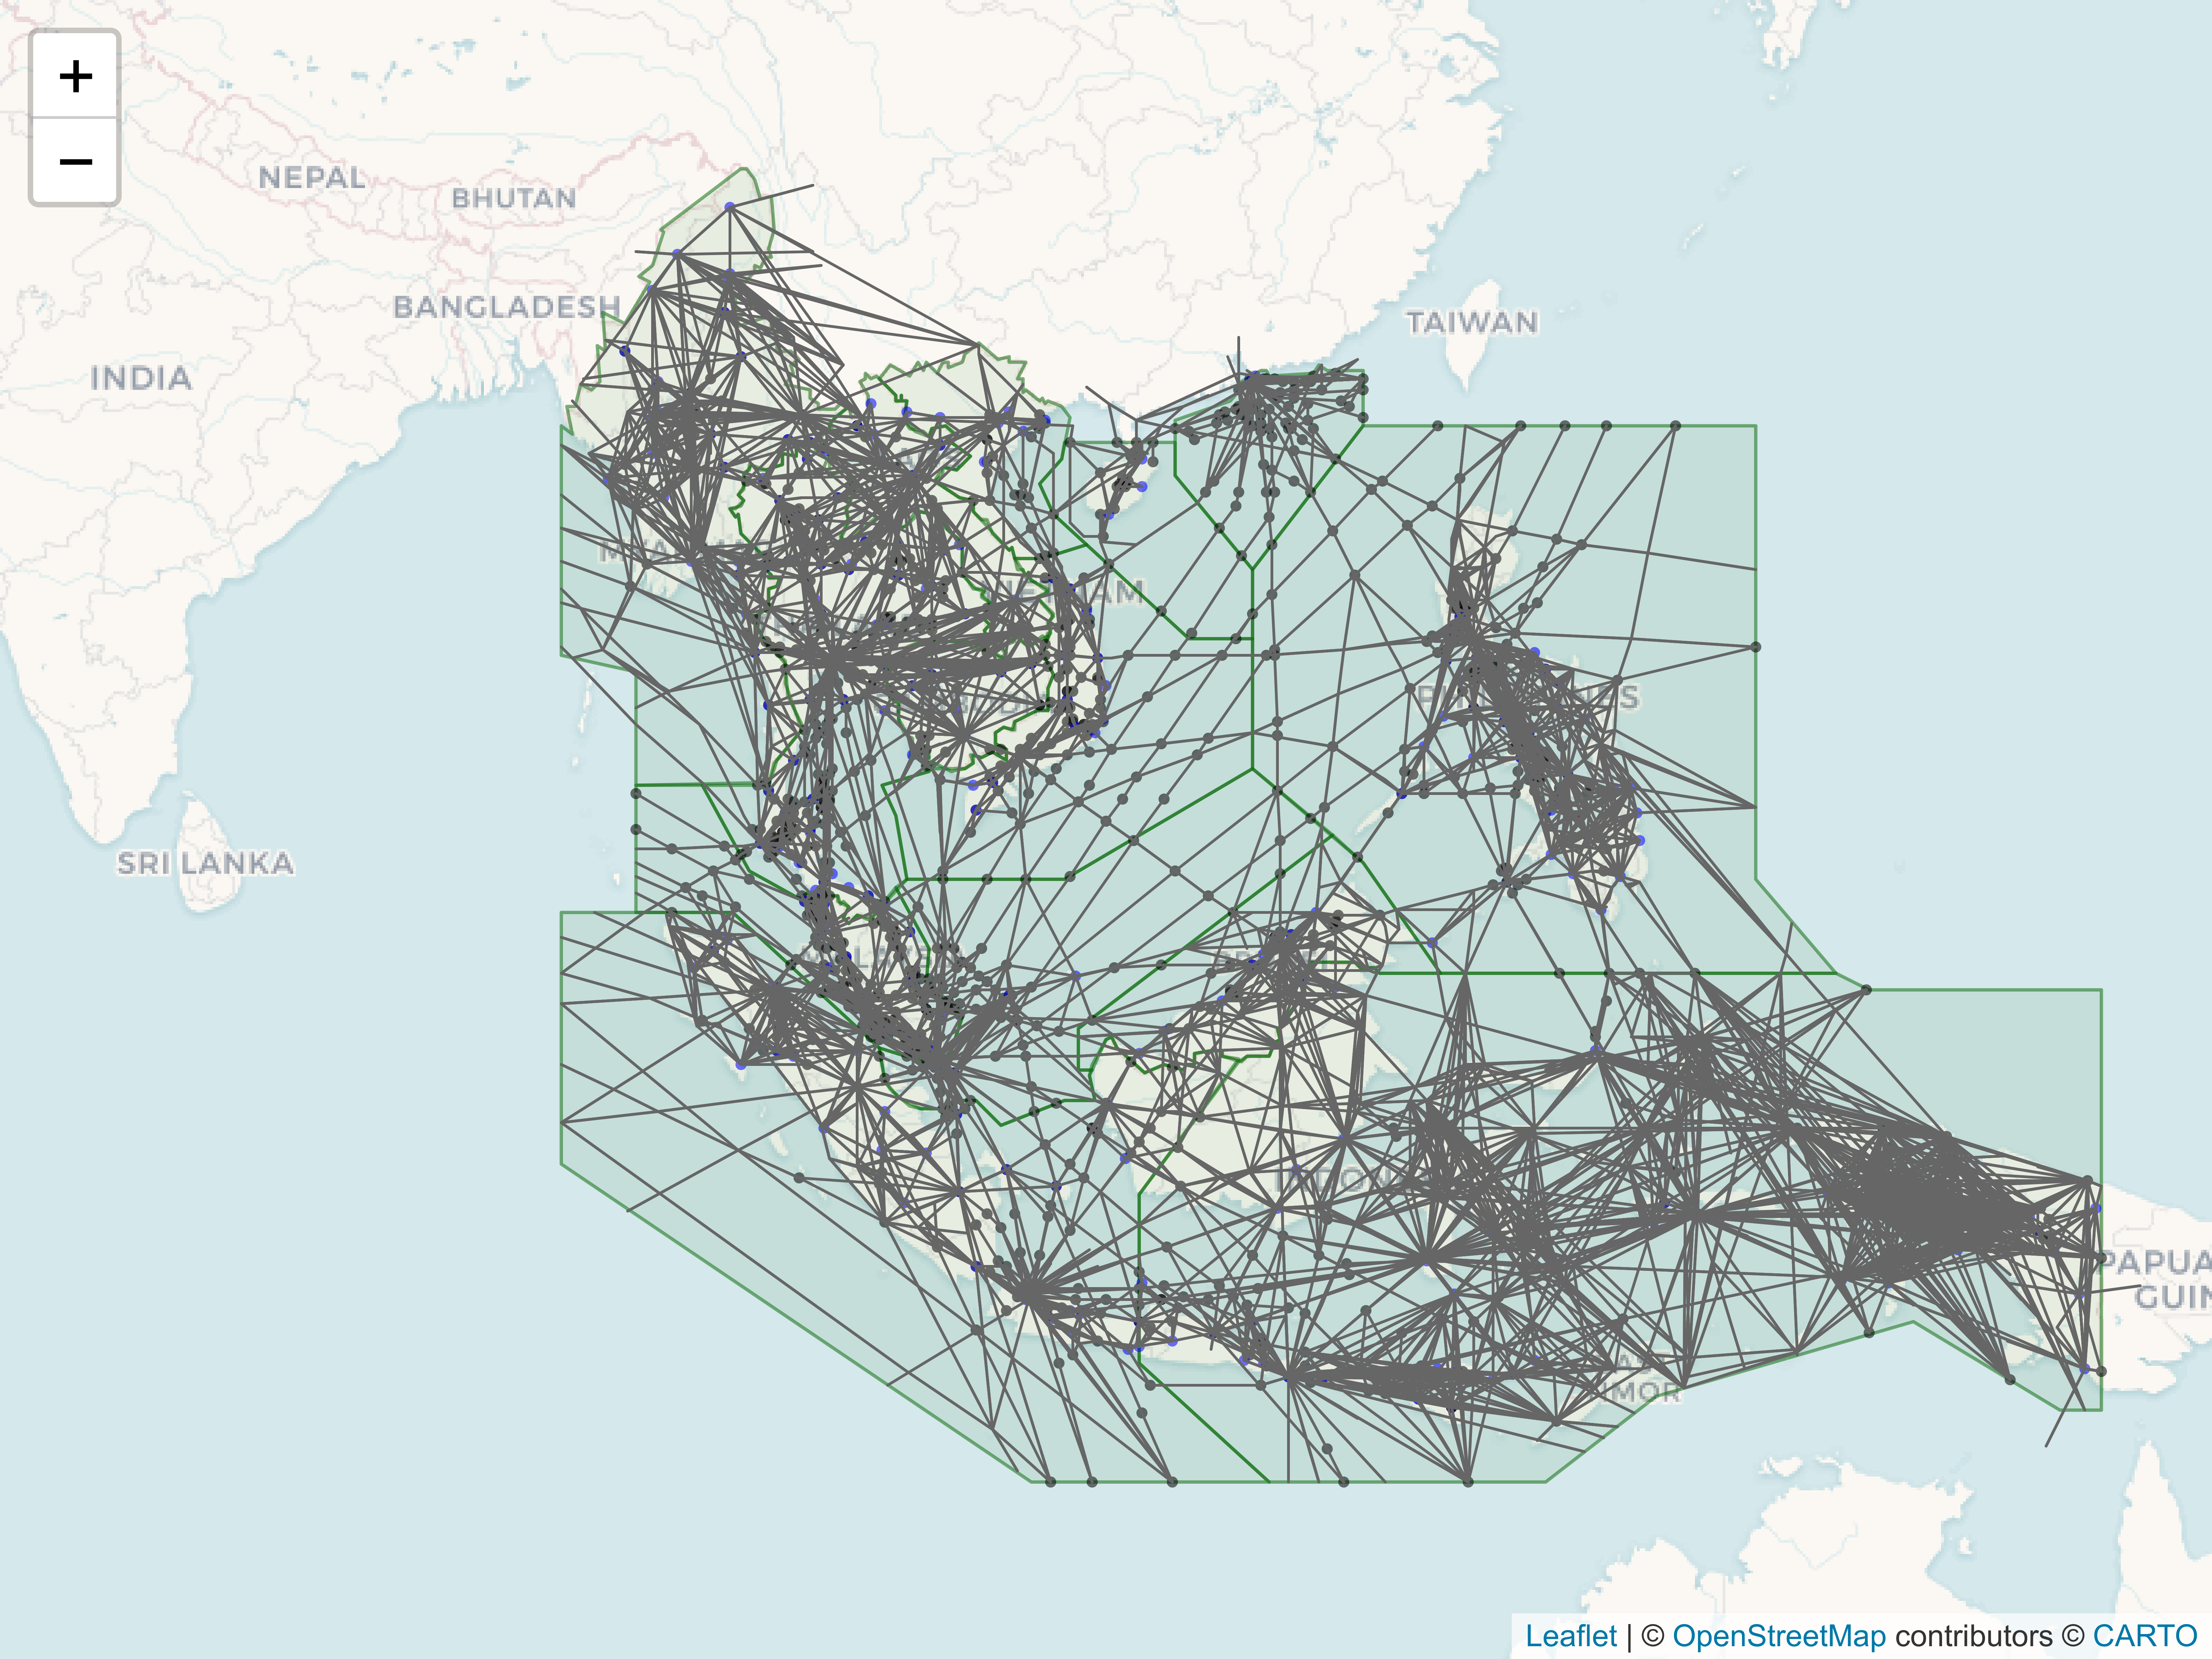
\includegraphics[width=0.8\textwidth]{Figures/FIR arcs.png}
    \caption{Flight Network Arcs Within the ASEAN Plus Region, with FIR Boundaries}
    \label{fig:arcs}
\end{figure}

We first formulate the optimization problem mathematically and provide a brief overview of the concepts central to mathematical optimization. Subsequently, we propose two algorithms to solve this problem, namely, Gradient Descent Ascent (GDA) and Simulated Annealing (SA). The formulations, results and additional considerations are included for each algorithm. Lastly, a summary of notation used in this chapter is provided in Section \ref{sec:WFRnotation}.

%--------------------------------------------------------
\section{Mathematical Formulation}
\label{sec:MF}
For each input dataset, we are given the initial flight trajectory for all flights in a single Flight Information Region (FIR). A flight trajectory consists of the path a flight will take, from entry to exit of this FIR, and the entry time of a flight into this FIR. We base our dataset on flight schedules (arrival and departure times) downloaded from OAG \parencite{OAG2024a}, and on flight plans derived using Dijkstra's shortest path algorithm applied to a representative network we created of air navigation routes for the ASEAN Plus region with connections to all origin-destination pairs in the flight schedule. Each flight plan specifies the sequence of nodes in our network traversed from its departure airport to its arrival airport. A node in the regional network may represent either an airport or a waypoint. For notational convenience, since the channels have been earlier determined by the AFR, a node in this chapter may refer to a waypoint, or a channel, one of arrival, departure, or mixed, at an airport. Each node in the regional network is designated by the FIR to which it belongs. Let $\mathcal{N}$ denote the set of nodes for the FIR of interest. For the FIR of interest, and each flight in the schedule, we restrict attention to the portion of the flight plan visiting nodes within that FIR. Let $\mathcal{F}$  denote the set of flight plans which intersect with $\mathcal{N}$. Let $P_f$ denote the sequence of nodes for flight $f\in\mathcal{F}$. We assume that the sequence is contiguous in terms of flight legs, that is, a flight does not leave an FIR and then re-enter the same FIR on a later leg of its journey. Let $j=1,2,\cdots,|P_f|$ index the nodes of the FIR-restricted flight plan in sequence and let $n_j\in\mathcal{N}$, or simply $n\in\ P_f$ when no confusion should exist, denote a particular node in the sequence.

We assume that each flight $f$ has an earliest time, $t_f^0$, at which it is estimated or known to have entered the airspace of the FIR. This could be the scheduled or actual departure time from an airport within the FIR, or it could be the estimated or known time the flight traversed the last node of a flight plan in an adjacent FIR, prior to entering the FIR of interest. Accordingly, we append a node $j=0$ to the beginning of each flight plan $P_f$ and associate with it the fixed time, $t_f^0$. No decision variables are associated with this node, so $n_0$ affects only the right-hand side of a constraint.

Similarly, we assume that each flight has a target time to land or otherwise exit the FIR. We associate this time with the last node in the flight plan and designate it as $\widetilde{t}_{|Pf|}$. In our simulation model, such times are initialized using flight schedules and updated dynamically by the airport flow regulator algorithm (for arrival times within the FIR) or, depending on the information sharing regime, passed in from the neighboring FIR if the flight transits out of the FIR of interest.

Each node $j=1,2,\cdots,|P_f|$, marks the \textit{end} of a flight leg. The first leg, $j=1$, can be thought of as the trip from the departure gate to the runway of the origin airport. We assume that the leg from $n_{j-1}$ to $n_j$ has a preferred duration ${\widetilde{d}}_{fj}$ particular to the flight $f$. The preferred duration of the first leg is zero (${\widetilde{d}}_{f1}=0$). In our simulation, we compute an ideal time profile for each trajectory as a whole from origin to destination with reference to the rate of ascent, cruising altitude, cruising speed, and rate of descent specific to the equipment type.  We compute an upper time profile (resp. lower time profile) by scaling the cruising speed down by 10\% (resp. up by 5\%).  For any leg, we use these three profiles to derive the preferred duration ${\widetilde{d}}_{fj}$, as well as the maximum ${\overline{d}}_{fj}$, and minimum ${\underline{d}}_{fj}$ leg durations. Appendix \ref{AppendixB} documents the calculations.

The trajectory of each flight $f\in\mathcal{F}$ is determined by the flight plan $P_f$, and for each node $j=1,2,\cdots,|P_f|$, the target time over (TTO) at the $j^{th}$ node in path $P_f$, denoted by $t_{fj}$.

For each node $j=1,2,\cdots,|P_f|$, we introduce two decision variables: a speed regulation factor, $\beta_{fj}$, and an extraordinary hold delay, $h_{fj}$. The TTO values are determined with the following forward recursion:
\begin{equation}
\label{eqn:fwrec1}
t_{f0}=t_f^0;
\end{equation}
\begin{equation}
\label{eqn:fwrec2}
t_{fj}=t_{fj-1}+h_{fj}+\beta_{fj}{\underline{d}}_{fj}+(1-\beta_{fj}){\overline{d}}_{fj};
\end{equation}
where $h_{fj}\geq0$ and $0\le\beta_{fj}\le1$ for all $j=1,2,\cdots,|P_f|$. Observe that increasing the speed regulation factor, $\beta_{fj}$, is associated with \textit{reducing} the duration of the $j^{th}$ leg. 

Also, observe that the extraordinary hold delay, $h_{fj}$, is applied to the trajectory after the flight has traversed node $j-1$. Thus, if we consider the first node in the FIR network, $j=1$, then the first node in the flight path, $j=0$, is a dummy node representing either a node in an adjacent FIR or an airport departure node. Consequently, $h_{f1}$ can be interpreted as a request to the neighboring FIR to hold a flight from entering the FIR of interest or a request to the airport scheduler to impose an additional ground delay on the flight.

We impose no upper limits on the extraordinary hold delay variables, $h_{fj}$. Instead, we introduce an extraordinary hold cost parameter $c_n$ associated with nodes $n\in\mathcal{N}$ to be applied to these delays. We anticipate the traffic manager would designate five classes of nodes with progressively increasing cost parameters: airport nodes (for which delays represent ground delays which cost less than airborne delays), neighboring FIR nodes (for which delays represent external airborne holding or requests for collaborative ground delays), nodes at entrances to designated holding areas within the FIR of interest, final approach nodes (for which delays represent vectoring), and all other waypoints (for which delays are strongly discouraged). In the experiments reported below, for example, we set the default values for holding costs for departure airports and final approach nodes at 1 and 10, respectively. Holding costs at all other nodes were set at 100.

The decision problem becomes a flow regulation problem when we impose flow constraints on the number of aircraft traversing specific nodes in the network. The flow capacity, and by extension, the minimum required separation time at each node, is determined in the same manner as in Section \ref{sec:envelope}. We consider simple flow constraints, such as an upper bound on the number of traversals by aircraft of any type through a given node during the current planning horizon. We enforce this by imposing a minimum separation time between any pair of flights whose flight path takes them through the constrained node. We let $\Delta_n$ denote the minimum separation time for flights traversing the node $n$.

To express the flow constraint generically, let $n$ denote a node with a flow constraint and let $f$ and $f'$ denote any pair of flights whose flight paths both include the node $n$. Let $j$ index node $n$ in $P_f$ and let $j'$ index node $n$ in $P_{f'}$. Let $\mathcal{C}$ denote the set of all such tuples $(f,f^\prime,j,j')$ of potential conflicts. Denote the corresponding TTOs at this node for these flights by $t_{fj}$ and $t_{f^\prime j^\prime}$, respectively. We require $\left|t_{fj}-t_{f^\prime j^\prime}\right|\geq\Delta_n$. We enforce this generically by defining a penalty function $\delta\left(\left|t_{fj}-t_{f^\prime j^\prime}\right|\right)$ for any strictly decreasing function $\delta(\cdot)$ and imposing the constraint:
\begin{equation}
    \delta\left(\left|t_{fj}-t_{f^\prime j^\prime}\right|\right)\le\delta\left(\Delta_n\right),
\end{equation}
where $n=n_j=n_{j^\prime}$.

An additional complication arises from the fact that these trajectories are updated in a rolling horizon fashion. At any point in time, some of the flights are en route. Consequently, not all TTOs are free to be modified. Our convention is that the TTO for the ending node of a leg becomes \textit{frozen} as soon as the simulation clock exceeds the TTO of the beginning node of that leg. That is, once an aircraft has transited a node, the TTO of the next node in its flight plan is frozen in time. The following proposition follows, which is a necessary condition for the forward TTO recursion.

\begin{proposition}
\label{prop:frozen}
    For any given trajectory, there does not exist a free leg before a frozen leg.
\end{proposition}
\begin{proof}
    From the definition of a frozen leg, the TTO at the end node of the leg must be immutable in the current and future time steps and current FIR of consideration. Assume we have a free leg before a frozen leg. From the definition of a free leg, we are allowed to modify its duration via changing its speed, or assigning a hold time. Say we increase the duration of this free leg. The forward TTO recursion would also increase the TTO at the end node of the frozen leg, hence a contradiction. The same argument can be made for decreasing the duration of the free leg.
\end{proof}

Let $\mathcal{R}$ denote the set of all flight legs:
\begin{equation}
\mathcal{R}=\bigcup_{f\in\mathcal{F}}\bigcup_{j=1}^{P_f}\left(f,j\right),
\end{equation}
and let $r=1,2,\cdots,\left|\mathcal{R}\right|$ index this set. Recall that we refer to a leg by its \textit{end} node (the first leg begins with path index $j=0$ and ends at $j=1$). Let $\overline{\mathcal{R}}$ denote the set of frozen legs and $\mathcal{R}^O=\mathcal{R}\backslash\overline{\mathcal{R}}$, the set of free legs. For a frozen leg, $(f,j)\in\overline{\mathcal{R}}$, let ${\overline{t}}_{fj}$ denote the fixed TTO of the end node of the frozen leg. We require, for all $(f,j)\in\overline{\mathcal{R}}$, 
\begin{equation}
    t_{fj}={\overline{t}}_{fj}.
\end{equation}

A flight is \textit{completed} from the perspective of the FIR of interest as soon as the last leg is frozen, and the current simulation clock exceeds the frozen TTO of the last leg. To ensure an active flight satisfies the minimum required separation from any completed flight, we will only archive a completed flight once all flight legs are completed, and the time now, is greater than the TTO of all flight legs belonging to this flight, plus its minimum required separation at each resource:
\begin{equation}
    t_{now} > t_{fj} + \delta_{fj} \quad \forall j\in P_f.
\end{equation}
Such flights are removed from consideration (i.e. deleted from $\mathcal{F}$). The remaining flights are considered to be \textit{active} even if all legs are frozen because there is at least one leg whose frozen time may affect separation requirements.


\begin{proposition}
    Removing separation constraints where both legs involved are frozen, does not increase the state space of which we can search for an optimal solution. The state space remains equivalent.
\end{proposition}
\begin{proof}
    For flight legs that are frozen, they may not be modified in the current time step and current FIR of consideration, effectively behaving as parameters rather than variables. Alternatively, we declare that freezing a leg is equivalent to removing this variable from the state space and converting it into a fixed parameter. For a separation constraint with both flight legs frozen, there are no variables involved, hence does not change the state space as constraints normally do. As there is no change to the state space, such separation constraints are redundant to the current optimization model, and we may remove them without modifying the state space.
\end{proof}

Given that the state space is equivalent, we can reduce the number of separation constraints by restricting attention to a subset of the separation constraints, $\mathcal{C}^I$, where at least one leg is free:
\begin{equation}
    \mathcal{C}^I=\left\{\left(f,f',j,j'\right)\in\mathcal{C}\ |\left(f,j\right)\in\mathcal{R}^O\mathrm{\ and/or}\left(f',j'\right)\in\mathcal{R}^O\right\}.
\end{equation}
Similarly, frozen legs are not subject to the forward TTO recursion. Let $j^O$ index the first leg in a given flight which is free. Then, the forward recursion
\begin{equation}
\label{eqn:fwrec3}
    t_{fj}=t_{f\left(j-1\right)}+h_{fj}+\beta_{fj}{\underline{d}}_{fj}+\left(1-\beta_{fj}\right){\overline{d}}_{fj}
\end{equation}
applies if and only if $j\geq j^O$. The recursion works due to Proposition \ref{prop:frozen}, as we observe that if a free leg existed prior to a frozen leg, any change in the speed or holding time of the earlier free leg would be propagated to the frozen legs and modify their TTOs. This would contradict the fact that the TTOs of frozen legs should be frozen.

In summary, we define the Waypoint Flow Regulation Problem (WFRP) as follows. The problem is to determine values for $\left(\beta_r,h_r\right)$ for all $ r\in\mathcal{R}^O$ to
\begin{equation}
\label{eqn:startlp}
    \underset{\beta,h}{\rm minimize} \ g(\beta,h) ={\sum_{f}\left(t_{f\left|P_f\right|}-{\widetilde{t}}_{f\left|P_f\right|}\right)^2+\sum_{\left(f,j\right)\in\mathcal{R}}{c_{n_j}h_{fj}}},
\end{equation}
subject to frozen leg constraints:
\begin{equation}
    t_{fj}={\overline{t}}_{fj}\ \forall\left(f,j\right)\in\overline{\mathcal{R}},
\end{equation}
initial node constraints:
\begin{equation}
    t_{f0}=t_f^0,\forall\ f\in\mathcal{F},
\end{equation}
trajectory constraints:
\begin{equation}
    t_{fj}=t_{fj-1}+h_{fj}+\beta_{fj}{\underline{d}}_{fj}+\left(1-\beta_{fj}\right){\overline{d}}_{fj},
\end{equation}
with decision variable bounds:
\begin{equation}
    h_{fj}\geq0,\mathrm{\mathrm{\ }and\ }0\le\beta_{fj}\le1,
\end{equation}
for all $f\in\mathcal{F}$ and $j=j^O,j^O+1,\cdots,\left|P_f\right|$;  and all separation requirements:
\begin{equation}
\label{eqn:endlp}
    \delta\left(\left|t_{fj}-t_{f^\prime j^\prime}\right|\right)\le\delta\left(\Delta_{n_j}\right),\forall\left(f,f^\prime,j,j^\prime\right)\in\mathcal{C}^I,
\end{equation}
where $n_j=n_{j'}$.

\begin{proposition}
\label{prop:feasible}
    A feasible solution to the WFRP is guaranteed to exist when the extraordinary hold times are unbounded from above.
\end{proposition}
\begin{proof}
    A sketch of the proof can be seen by setting every speed regulation variable to achieve the preferred duration, ${\widetilde{d}}_{fj}$, and every extraordinary hold time variable to zero except for the first free leg of each flight: $h_{fj}=0,\forall j\geq j^O$. The free TTOs for each flight can be shifted arbitrarily far to the right by increasing $h_{fj^o}$ for that flight. Flights can be considered in turn and shifted sufficiently to the right to satisfy separation constraints with all previously considered flights.
\end{proof}

Next, we define the terms local minima and global minimum, as these definitions are required in Proposition \ref{prop:localglobal}. We denote the feasible region of the WFRP $\mathcal{W}$, and the region near the current solution as a ball centered at $(\overline{\beta},\overline{h})$ as:
\begin{equation}
    B(\overline{\beta},\overline{h}, \epsilon) = \{\beta|\Vert \beta - \overline{\beta} \Vert \leq \epsilon, h|\Vert h - \overline{h} \Vert \leq \epsilon\}.
\end{equation}
\begin{definition}
$(\beta,h)$ is a local minimum of the WFRP if there exists $\epsilon > 0$ such that $g(\beta,h) \leq g(\beta',h') \ \forall (\beta',h')\in B(\beta,h,\epsilon)\cap\mathcal{W}$.
\end{definition}

\begin{definition}
$(\beta,h)$ is a global minimum of the WFRP if $g(\beta,h) \leq g(\beta',h') \ \forall (\beta',h')\in \mathcal{W}$.
\end{definition}

\begin{definition}
\label{def:convex}
A function $f$ is convex if:
\begin{equation}
    f(tx+(1-t)y)\leq tf(x)+(1-t)f(y)
\end{equation}
for all $x,y\in \textrm{dom} f$ and all $t\in[0,1]$.

For sets, this may be restated as: A set $C$ is convex if the line segment between any two points in $C$ lies in $C$:
\begin{equation}
    tx_1 + (1-t)x_2 \in C
\end{equation}
$\forall x_1, x_2 \in C, \forall t\in[0,1]$

\end{definition}

\begin{proposition}
\label{prop:localglobal}
    The WFRP is a non-convex problem.
\end{proposition}
\begin{proof}
    The separation constraint involves an absolute function on the TTOs, \\
    $\delta\left(\left|t_{fj}-t_{f^\prime j^\prime}\right|\right)\le\delta\left(\Delta_n\right)$. This causes the feasible region to be disjoint. We can draw a line between two points, each from a disjoint segment and it will lie outside the feasible set, hence using Definition \ref{def:convex}, we have shown the WFRP is a non-convex problem.
\end{proof}

Given that the WFRP is a non-convex problem, local minima may not equal to the global minimum. We illustrate this concept with an example, by simplifying the WFRP to two flight legs, $t_1$ and $t_2$, with preferred times $\widetilde{t}_1 = 0$, $\widetilde{t}_2 = 3$, and separation constraint $e^{-|t_1-t_2|}\leq e^{-5}$, using the $\delta(\cdot)$ function defined in Section \ref{sub:GDApenalty}. Note that in the WFRP, the values representing time are positive, but we allow them to be negative for this example. Also, we simplify the notation by using $t=(t_1,t_2)$.

In Figure \ref{fig:conset}, the concentric circles indicate the level sets of $f(t) = (t_1-0)^2 + (t_2-3)^2$, the function which mimics deviation from preferred time, of which we are trying to minimize. The area shaded in light blue is the feasible set, of which the two aircraft obey separation requirements. The second-largest circle $f(t)=32$, is a local minimum at $(4,-1)$, as perturbing $t_1$ or $t_2$ by a small value $\epsilon$ will lead to a larger value of $f(t)$, as represented by the largest circle $f(t) = 35$. However, $f(t)=32$ is not a global minimum as there exists another local minimum where the circle $f(t)=2$ touches the feasible set at $(-1,4)$ and $2<32$. Applying this analogy to the WFRP, we state that \textit{local minima exist when aircraft obey the separation constraints, with TTO as close to the preferred time as possible, but are in a non-optimal sequence}. A global minimum exists when aircraft obey the separation constraints, with TTO as close to the preferred time as possible, and are optimally sequenced.

\begin{figure}[htbp]
    \centering
    \includegraphics[width = \textwidth]{Figures/convex set.pdf}
    \caption{Geometrical View of Local and Global Minima}
    \label{fig:conset}
\end{figure}

The existence of local minima for the WFRP is an important consideration in selecting optimization heuristics, given that a local minimum could be suboptimal, and potentially possess an arbitrarily large optimality gap from the global minimum.

%--------------------------------------------------------
\section{Description of Mathematical Optimization}
\label{sec:opti}
The modern form of mathematical optimization, as it is known today, began around the time of Newton, Gauss, Fermat, and Lagrange, in the fifteenth and sixteenth centuries. Some of their contributions to the field of optimization are the method of Lagrange multipliers, Newton’s method, Fermat’s theorem, and Gauss-Newton algorithm. Mathematical optimization is a method of obtaining the best possible outcome, based on the available choices. Today, it plays a huge role in many industries, not limited to transportation, energy, finance, scheduling, routing, and telecommunications \parencite{Festa2014}. As seen in the discussion of ATFM in Chapter \ref{chap2}, airspace problems are no exception to this, where mathematical optimization has been extensively used to improve the efficiency of aviation operations, and have been proven successful in increasing the airspace and runway capacity. 

More formally, mathematical optimization is the process of breaking down a problem into either a discrete or continuous set space of inputs. This set space of inputs is commonly referred to as decision variables. From these inputs, subject to further constraints, select the input set which returns the optimal values for zero or more objective functions. For a maximization problem (resp. minimization), given a set of variables $x\in\mathbb{R}^n$ and an objective function $f(x)$, we aim to find $x_0$ for which $f(x_0)\geq f(x)$ (resp. $f(x_0)\leq f(x)$) for all $x\in S$ where $S$ is the subset of $\mathbb{R}^n$ which fulfills the specified set of constraints. 

Problems with no objective function are also known as feasibility problems, where the goal is to find any values for the variables such that all constraints are satisfied. In other situations, there may be more than one objective function. For these problems, we may search for a Pareto optimal set of possible solutions or, more commonly, use a multi-objective optimization tool such as the popular Non-dominated Sorting Genetic Algorithm (NSGA-II) \parencite{Deb2002}.

The characterization of inputs, constraints and objective functions are critical to determining the final outcome. For example, the least squares regression problem is well-defined with objective to minimize the sum of squared residuals, where otherwise minimizing the residuals itself would give an incorrect result since the case of which large positive and negative residuals balance each other out would be considered optimal. This is often the most important phase where the decision has substantial impact on the interpretability and application of the problem and its corresponding solution.

There are two main categories of algorithms designed for mathematical optimization: exact methods and heuristic methods. As the name suggests, exact methods return the optimal solution, which can be proven to be globally optimal. Common approaches include Branch and Bound, Integer Programming, Linear Programming and Dynamic Programming. The strength of exact methods lies in its ability to obtain the global optimal. However, a number of problems, for example, the Traveling Salesman Problem, Flow Shop Scheduling Problem, and minimum k-cut problem, are NP-complete, for which no polynomial-time algorithm is currently known. This implies obtaining the global optimum within a reasonable computational time frame when the problem size is large is not feasible. To answer these important problems, research has been directed towards heuristic methods, which return a solution, with no guarantee of achieving the global optimal and are often, instead, compared against other solutions \parencite{Festa2014}. The strength of heuristic methods lies in their computational efficiency and ability to achieve solutions within an acceptable optimality gap. They have been used extensively in place of exact algorithms for problems that are too large for exact algorithms to provide a solution for real time decision-making. Some examples of heuristic methods are Simulated Annealing, Genetic Algorithms, Gradient Descent and Neural Networks. 

The WFR is a nontrivial optimization problem because it involves sequencing flights at nodes, of which is combinatorial in nature. A natural choice of optimization model for smaller instances would be to consider using an integer program, as done in the papers \parencite{Balakrishnan2014, Tan2021}. However, in the broader context of our research, we are constrained by computational time of the algorithm as we require solving a dozen or so FIRs at each time step of our simulation, with thousands of flights over a 24-hour period. For this reason, we pursue a heuristic approach to solving the WFRP by means of GDA and SA, both of which are presented in the next few sections. We will then discuss which heuristic is most suited for the WFRP and provide our choice of heuristic for the simulator to conclude the chapter.


%--------------------------------------------------------
\section{Gradient Descent Ascent}
\label{sec:GDA}
The Gradient Descent (GD) family of algorithms is one of the most widely used algorithms for unconstrained mathematical optimization. It makes use of the first order derivative of some differentiable multivariate function, guiding the variables against the direction of the gradient, leading to a local minimization of the objective function. GD is used extensively in the field of Deep Learning, where every state-of-the-art Deep Learning library contains various implementations and algorithms of GD \parencite{Ruder2016}. Some of the most popular extensions include Adam, which combines AdaGrad and RMSProp, designed to work well with sparse gradients and non-stationary settings \parencite{Kingma2014}, and Stochastic Gradient Descent, designed to work well in the context of high dimensional optimization. Gradient Descent Ascent (GDA) is another flavor of GD, which sees applications in different fields, being more commonly applied in Generative Adversarial Networks and Reinforcement Learning. One key strength of the GDA lies in its capacity to handle constrained optimization problems through Lagrangian duality. Therefore, in this paper, we leverage GDA’s advantages to solve the WFR, which is formulated as a constrained optimization problem.

For a minimization problem, our augmented objective function is $\underset{x}{\min}\ \underset{\lambda}{\max}\ \mathcal{L}\left(x,\lambda\right)=f\left(x\right)+\lambda^Tg\left(x\right)$, subject to $\lambda\geq 0$. Here, $f(x)$ denotes the objective function, and $g(x)$ denotes set of constraint functions. We can think of this method as penalizing the objective function when $g\left(x\right)\geq 0$ as $\lambda^Tg\left(x\right)$ will be greater than zero, bringing us further away from our goal of minimizing the function with respect to $x$. Alternatively, a geometrical view is noticing how the term $\lambda^Tg\left(x\right)$ imposes supporting hyperplanes $g_i\left(x\right)\leq 0$ onto the feasible set, which shrinks the set of values which $x$ will take on, and with appropriate step sizes, we will eventually have $x\in S$.

The GDA heuristic is described in Algorithm \ref{alg:GDA}.
\begin{algorithm}
\setstretch{1.3}
\caption{Gradient Descent Ascent}
\label{alg:GDA}
$x^{(1)}\gets x_0$;\\
$\lambda^{(1)}\gets \lambda_0$;\\
\For{$i\gets1$ \KwTo $N$}{
    compute $\frac{\partial\mathcal{L}}{\partial x}$ and $\frac{\partial\mathcal{L}}{\partial\lambda}$;
    
    update $x^{\left(n+1\right)}=x^{\left(n\right)}-\eta\frac{\partial\mathcal{L}}{\partial x}$ and $\lambda^{\left(n+1\right)}=\lambda^{\left(n\right)}+\theta\frac{\partial\mathcal{L}}{\partial\lambda}$.
}
\end{algorithm}

For Algorithm \ref{alg:GDA}, let $x_0$ and $\lambda_0$ represent arbitrary initial values of $x$ and $\lambda$ respectively, and $N$ denote the number of iterations. Let $x^{(n)}$ for any variable $x$, represent the value of $x$ at the $n^{th}$ iteration of the GDA heuristic. Also, let $\eta$ and $\theta$ represent the step size vector for the primal vector $x$ and dual vector $\lambda$ respectively.
%--------------------------------------------------------
\subsection{Choice of Penalty Function}
\label{sub:GDApenalty}
Our choice of the penalty function $\delta(\cdot)$ for use in the separation constraints is driven by the decision to use the GDA algorithm. In general, we want $\mathcal{L}\left(x,\lambda\right)$ to be strongly convex with respect to the primal vector $x$. A strongly convex function possesses the property where if the gradient at a point is close to zero, the point is close to its locally optimal value. Boyd and Vandenberghe \parencite{Boyd2004} provides a proof of convergence for descent methods on strongly convex functions. We selected the Laplace function, $\delta\left(x\right)=e^{-|x|}$, plotted in Figure \ref{fig:laplace} for this reason, as it is strongly convex on both the positive and negative $x$ domain. We also considered the reciprocal of squared deviation $\delta(x)=\frac{1}{x^2}$ but anticipated that its lack of continuity at zero would lead to extreme behavior.

A plot of the Laplace function is given in Figure \ref{fig:laplace}, with a sample required separation of two units. In the figure, when the $x$ values are close to zero, within the red zone, the constraint is violated. Otherwise, when the $x$ values are further from zero, within the blue zone, the constraint is satisfied.

\begin{figure}[htbp]
    \centering
    \includegraphics[width = 0.6\textwidth]{Figures/laplace.pdf}
    \caption{Graph of $\delta(x)=e^{-|x|}$, With a Sample Required Separation of Two Units}
    \label{fig:laplace}
\end{figure}


%--------------------------------------------------------
\subsection{Lagrangian Relaxation}
\label{sub:GDAlagrange}

We associate the dual variable $\lambda_{f,f^\prime,n_j}$, where $n_j=n_{j^\prime}$, with each separation constraint $\left(f,f^\prime,j,j^\prime\right)\in\mathcal{C}^I$, and form the Lagrangian function $\mathcal{L}\left(\beta,h,\lambda\right)$ as follows:
\begin{equation}\begin{split}
\mathcal{L}\left(\beta,h,\lambda\right)&=\sum_{f}\left(t_{f\left|P_f\right|}-{\widetilde{t}}_{f\left|P_f\right|}\right)^2+\sum_{\left(f,j\right)\in\mathcal{R}}{c_{n_j}h_{fj}}\\
&+\sum_{\left(f,f^\prime,j,j^\prime\right)\in\mathcal{C}^\prime}{\lambda_{f,f^\prime,n_j}\left(\delta\left(\left|t_{fj}-t_{f^\prime j^\prime}\right|\right)-\delta\left(\Delta_{n_j}\right)\right)}.
\end{split}\end{equation}
Except for the decision variable bounds, all other constraints are expressed as equalities and hence can be eliminated through substitution. The dualized WFRP is thus to find primal vectors $(\beta,h)$ and dual vector $\lambda$ to solve:
\begin{equation}
    \underset{\lambda}{\max}\ \underset{\beta,h}{\min}\ \mathcal{L}\left(\beta,h,\lambda\right)
\end{equation}
subject to the decision variable bounds:
\begin{equation}
    h_{fj}\geq0,\mathrm{\ and\ }0\le\beta_{fj}\le1,
\end{equation}
for all $f\in\mathcal{F}$ and $j=j^O,j^O+1,\cdots,\left|P_f\right|$. 


%--------------------------------------------------------
\subsection{Gradient Descent Ascent Applied to the Waypoint Flow Regulator Problem}
\label{sub:GDAapply}

We compute the partial derivatives of the Lagrangian as:
\begin{equation}\begin{split}
\frac{\partial\mathcal{L}}{\partial\beta_{fj}}& =({\underline{d}}_{fj}-{\overline{d}}_{fj})\Bigg(2\left(t_{f\left|P_f\right|}-{\widetilde{t}}_{f|P_f|}\right)
\\&-\sum_{(f,f',j,j')\in\mathcal{C}^I}{\lambda_{f,f',n_j}\delta\left(\left|t_{fj}-t_{f^\prime j^\prime}\right|\right)sgn\left(t_{fj}-t_{f'j'}\right)}
\\&+\sum_{(f',f,j,j')\in\mathcal{C}^I}{\lambda_{f',f,n_j}\delta\left(\left|t_{fj}-t_{f^\prime j^\prime}\right|\right)sgn\left(t_{f' j'}-t_{fj}\right)}\Bigg)\ \forall(f,j)\in\mathcal{R};
\end{split}\end{equation}

\begin{equation}\begin{split}
\frac{\partial\mathcal{L}}{\partial h_{fj}}& =\Bigg(2\left(t_{f\left|P_f\right|}-{\widetilde{t}}_{f|P_f|}\right)
\\&-\sum_{(f,f',j,j')\in\mathcal{C}^I}{\lambda_{f,f',n_j}\delta\left(\left|t_{fj}-t_{f^\prime j^\prime}\right|\right)sgn\left(t_{fj}-t_{f'j'}\right)}
\\&+\sum_{(f',f,j,j')\in\mathcal{C}^I}{\lambda_{f',f,n_j}\delta\left(\left|t_{fj}-t_{f^\prime j^\prime}\right|\right)sgn\left(t_{f' j'}-t_{fj}\right)}\Bigg)+c_{n_j}\ \forall(f,j)\in\mathcal{R};
\end{split}\end{equation}

\begin{equation}
    \frac{\partial\mathcal{L}}{\partial\lambda_{f,f^\prime,n_j}}=\delta\left(\left|t_{fj}-t_{f^\prime j^\prime}\right|\right)-\delta\left(\Delta_{n_j}\right)\ \forall\left(f,f^\prime,j,j^\prime\right)\in\mathcal{C}^I.
\end{equation}

Our aim is to minimize the Lagrangian with respect to $\beta$ and $h$, and maximize the Lagrangian with respect to $\lambda$, with the following bounds:
\begin{equation}
    0\leq\beta_{fj}\leq 1\ \ \forall\left(f,j\right)\in\mathcal{R};
\end{equation}
\begin{equation}
    0\leq h_{fj}\ \ \forall\left(f,j\right)\in\mathcal{R};
\end{equation}
\begin{equation}
    0\leq\lambda_{f,f^\prime,n_j}\ \ \forall\left(f,f^\prime,j,j^\prime\right)\in\mathcal{C}^I.
\end{equation}
We do this by updating the variables $\beta,h,\lambda$, with step sizes $\eta,\iota,$ and $\mu$ as follows:
\begin{equation}
    \beta^{\left(n+1\right)}=\min \Biggl\{1, \max \biggl\{ 0, \beta^{\left(n\right)}-\eta\frac{\partial\mathcal{L}\left(\beta^{\left(n\right)},h^{\left(n\right)},\lambda^{\left(n\right)}\right)}{\partial\beta} \biggl\} \Biggl\};
\end{equation}
\begin{equation}
    h^{\left(n+1\right)}=\max\biggl\{0, h^{\left(n\right)}-\mu\frac{\partial\mathcal{L}\left(\beta^{\left(n\right)},h^{\left(n\right)},\lambda^{\left(n\right)}\right)}{\partial h} \biggl\};
\end{equation}
\begin{equation}
\lambda^{\left(n+1\right)}=\max \biggl\{0, \lambda^{\left(n\right)}+\iota\frac{\partial\mathcal{L}\left(\beta^{\left(n\right)},h^{\left(n\right)},\lambda^{\left(n\right)}\right)}{\partial\lambda} \biggl\};
\end{equation}
where $x^{\left(n\right)}$  for any variable $x$ represents the value of $x$ at the $n^{th}$ iteration of the GDA heuristic.

Here, note that the penalty function $\delta(x)=e^{-|x|}$ is non-differentiable at $x=0$. Many techniques exist to overcome such a challenge, particularly within the machine learning community. One example is an adaptation of the ReLU gradient \parencite{Bai2022}, of which gradient is piecewise determined as:
\begin{equation}
    f'(x) = 
    \begin{cases}
        0 & \text{if } x < 0,\\
        1  & \text{if } x \geq 1.
    \end{cases}
\end{equation}
This can be adapted to our GDA algorithm by adding a case for $x = 0$. In this case, we can assign an arbitrary value to the derivative which will lead to a change in the TTO of the overlapping flights, and such a change will separate the two flights that are in conflict.

Another option is a clip function, commonly used to prevent excessive jumps in variable values \parencite{DeepSeekAI2025}, particularly when computing the gradient. The clip function is defined as:
\begin{equation}
    \text{clip}(x, \overline{x}, \underline{x}) = \min\{\max\{x,\underline{x}\}, \overline{x}\}.
\end{equation}
Here, the clip function bounds a value between a particular minimum and maximum value. Applied to our GDA, this would prevent the TTO from changing by an excessive amount at each time step. We have opted for the clip function to deal with the non-differentiability of the penalty function. Given that the primal and dual variables are already bounded, where $0\leq\beta\leq 1$, $0\leq h$, and $0\leq \lambda$, we only need to clip off any large increments to both $h$ and $\lambda$. The upper limits for the changes in $h$ and $\lambda$ at each iteration were set to 500 and 10,000, respectively. The limit for $h$ was chosen to reflect a reasonable maximum adjustment in the holding time per iteration. In contrast, a substantially larger limit was assigned to $\lambda$ because it is not a primal variable and does not directly influence the objective function. This allows for significant variation in $\lambda$ without compromising computational stability.

Choosing suitable step sizes is both an art and a science: too large and our GDA heuristic will oscillate, too small and convergence will be slow. In addition to choosing a step size for each variable, we must implement a scheme to shrink the step sizes. This is because oscillation occurs with constant step size for non-strongly concave problems, particularly when there is interaction between the variables over which we are maximizing and minimizing \parencite{Liang2018}. 

To mitigate the impact of these oscillations, we geometrically shrink the step size every 50 iterations, with the total number of iterations for the GDA heuristic set at 500. For both $\beta$’s and $h$’s step sizes, we multiply them by 0.6 once every 50 iterations have been completed. Note here that we do not multiply the step size for $\lambda$ with a shrinking factor, because if we reduce the step size $\iota$, when two flights get too close towards the end of the algorithm, then $\lambda$ will increase too slowly to have an impact on the variables that determine the flight schedule $\beta$ and $h$. This would likely lead to conflicts as flights tend toward their preferred exit time, or reduce holding time, unless the penalty ($\lambda$) imposed for conflicts is sufficiently large.

The initial values of step sizes are set according to the general principle to have the change, at each iteration, for $\beta$ and $h$ to be of magnitude 0.1 and 100 respectively, and for $\lambda$ to be of magnitude 1. To that end, with some trial and error, we set $\eta=1/10000$, $\mu=2$ and  $\iota_{fj}=1000/\left(\delta\left(\Delta_{n_j}\right)\right)^2$. We sought to make $\iota_{fj}$ to be unique to each flight leg to normalize the step size with respect to $\Delta_{n_j}$, as our experimental results demonstrated that not scaling $\iota$ according to required separation led to unevenness in number of iterations to converge. This occurred because the variable $\lambda_{f,f',n_j}$ corresponding to a constraint with large separation time will increase significantly slower than $\lambda_{f,f',n_j}$ corresponding to a small separation time, particularly when exponentiation is involved. These parameters have been found to produce the least number of conflicts when GDA was run across all FIR datasets generated by our simulator.

%--------------------------------------------------------
% \subsection{Results}
% \label{sub:GDAres}
% For the results in this section, Section \ref{sec:SA} and Chapter \ref{chap7}, the data sources follow the description in Section \ref{sec:datasources}.

% The dataset used for our experimental runs are published flight plans for flights arriving or departing from the ASEAN Plus region on 1 Oct 2023. For the results below, we reiterate that a flight is completed from the perspective of the FIR of interest as soon as the last leg is frozen, and the current simulation clock exceeds the frozen TTO of the last leg. We model a look ahead period of two hours, such that all flights with at least one active or frozen leg during the next two hours will be added into consideration for the optimization algorithm. For flights with all legs frozen, we still include them as other flights must still maintain the required separation from these frozen flights where possible. We set the time shift for the sliding window at five minutes, that is, we optimize flights for the next two hours, at every five minute interval. As such, for the results in Tables \ref{tab:GDRegular} and \ref{tab:GDReduced}, we optimize flights arriving or departing from the ASEAN Plus region on 1 Oct 2023, from 04:00:00 to 06:00:00 UTC, or 12:00:00 to 14:00:00 GMT +8, which is a peak period for flights in the ASEAN Plus region.

% The regular airspace capacity is determined quantitatively using OAG data to obtain the capacity envelope for the number of arrivals, departures and total operations at each airport node, and the maximum number of operations was used as the capacity for waypoint nodes. These computations are similar to the method employed in \parencite{Tan2021}. The reduced airspace capacity is computed by synthetically reducing the original airspace capacity at arrival and departure nodes to 0.80 of their original levels, rounded up to an integer value. These capacity values are then used to compute the required separation time between aircraft by dividing the number of seconds in an hour by the number of flights in an hour. 
% % The total number of active flights for the regular and reduced capacity airspace scenarios are fixed at 2897 and 2990 respectively.

% The PC specifications used to run all the code are Intel(R) Core(TM) i7-10875H CPU @ 2.30GHz with 16 GHz installed RAM. The code was written in R for GDA, and Java for SA. The main results are presented in Tables \ref{tab:resultsGDA} and \ref{tab:resultsSA}. The results tables contain the following columns:

% \begin{itemize}
%     \item \textbf{FIR}: The FIR under consideration.
%     \item \textbf{No. Of Legs}: The total number of flight legs under consideration in the FIR.
%     \item \textbf{No. Of Free Legs}: The total number of flight legs that are free to be modified by the optimization heuristic. These are the flight legs that are visible to the FIR, and the associated aircraft has not transited over.
%     \item \textbf{No. Of Active Flights}: The total number of active flights under consideration in the FIR.
%     \item \textbf{No. Of Conflicts}: The number of conflicts remaining, that fail to observe the required separation time, summed over all FIRs in the ASEAN Plus region.
%     \item \textbf{Sum Of Absolute Deviation}: The sum of absolute deviation time from preferred time at the last leg of flight in the FIR, summed over all FIRs in the ASEAN Plus region. $\sum_{f}\left|t_{f\left|P_f\right|}-{\widetilde{t}}_{f\left|P_f\right|}\right|$. Expressed in hours.
%     \item \textbf{Mean Absolute Deviation}: The sum of absolute deviation, divided by the number of active flights. Recomputed in the last row \textbf{TOTAL}, as the total sum of absolute deviation divided by the total number of active flights. Expressed in hours. 
%     \item \textbf{Run Time}: Computational run time taken to optimize flight trajectories in the FIR, computed using the R library microbenchmark. Expressed in seconds.
% \end{itemize}

% \begin{table}[htbp]
%   \centering
%   \caption{Results for Gradient Descent Ascent on Regular Capacity Airspace on 1 Oct 2023 04:00:00 UTC Within ASEAN Plus Region Dataset}
%     \begin{tabular}{@{}m{1.2cm}m{1.1cm}m{1.1cm}m{1.4cm}m{1.2cm}m{2.2cm}m{2.2cm}m{1.4cm}@{}}
%     \toprule \toprule
%     FIR   & {No. of Legs} & {No. of Free Legs} & {No. of Active Flights} & {No. of Conflicts} & {Sum of Absolute Deviation (h)} & {Mean Absolute Deviation (h)} & {Run Time (s)} \\
%     \midrule \midrule
%     VTBB  & 1041  & 247   & 322   & 0     & 45.40 & 0.14  & 0.69 \\
%     WMFC  & 966   & 226   & 280   & 3     & 67.90 & 0.24  & 0.68 \\
%     WSJC  & 731   & 182   & 287   & 4     & 71.45 & 0.25  & 0.68 \\
%     WBFC  & 227   & 63    & 87    & 0     & 5.88  & 0.07  & 0.37 \\
%     WIIF  & 1006  & 313   & 386   & 2     & 83.40 & 0.22  & 0.85 \\
%     VVTS  & 1148  & 345   & 263   & 4     & 83.03 & 0.32  & 0.83 \\
%     ZJSA  & 646   & 145   & 299   & 1     & 89.00 & 0.30  & 0.62 \\
%     VHHK  & 744   & 308   & 224   & 1     & 118.10 & 0.53  & 0.83 \\
%     RPHI  & 1187  & 440   & 263   & 0     & 41.51 & 0.16  & 0.78 \\
%     VDPP  & 122   & 16    & 41    & 0     & 6.09  & 0.15  & 0.37 \\
%     WAAF  & 1008  & 352   & 457   & 0     & 85.60 & 0.19  & 0.75 \\
%     VLVT  & 113   & 21    & 79    & 0     & 11.32 & 0.14  & 0.37 \\
%     VVVV  & 776   & 208   & 177   & 1     & 51.50 & 0.29  & 0.71 \\
%     VYYF  & 255   & 86    & 107   & 0     & 10.84 & 0.10  & 0.40 \\
%     \midrule
%     \textbf{TOTAL} & \textbf{9970}  & \textbf{2952}  & \textbf{3272}  &
%     \textbf{16}    & \textbf{771.02} & \textbf{0.24}  & \textbf{8.93} \\
%     \bottomrule \bottomrule
%     \end{tabular}%
%   \label{tab:GDRegular}%
% \end{table}%

% \begin{table}[htbp]
%   \centering
%   \caption{Results for Gradient Descent Ascent on Reduced Capacity Airspace on 1 Oct 2023 04:00:00 UTC Within ASEAN Plus Region Dataset}
%     \begin{tabular}{@{}m{1.2cm}m{1.1cm}m{1.1cm}m{1.4cm}m{1.2cm}m{2.2cm}m{2.2cm}m{1.4cm}@{}}
%     \toprule \toprule
%     FIR   & {No. of Legs} & {No. of Free Legs} & {No. of Active Flights} & {No. of Conflicts} & {Sum of Absolute Deviation (h)} & {Mean Absolute Deviation (h)} & {Run Time (s)} \\
%     \midrule \midrule
%     WIIF  & 1049  & 333   & 410   & 1     & 153.85 & 0.38  & 0.95 \\
%     WAAF  & 1077  & 363   & 480   & 4     & 135.58 & 0.28  & 0.75 \\
%     ZJSA  & 601   & 123   & 293   & 0     & 102.72 & 0.35  & 0.56 \\
%     WSJC  & 739   & 205   & 286   & 4     & 103.20 & 0.36  & 0.72 \\
%     WMFC  & 965   & 209   & 282   & 2     & 104.57 & 0.37  & 0.68 \\
%     VVTS  & 1112  & 348   & 267   & 1     & 117.76 & 0.44  & 0.83 \\
%     VHHK  & 765   & 337   & 232   & 0     & 188.41 & 0.81  & 0.85 \\
%     RPHI  & 1167  & 436   & 262   & 0     & 58.13 & 0.22  & 0.75 \\
%     VVVV  & 795   & 233   & 183   & 1     & 93.10 & 0.51  & 0.74 \\
%     VLVT  & 111   & 17    & 77    & 0     & 16.91 & 0.22  & 0.36 \\
%     VTBB  & 1011  & 223   & 328   & 1     & 91.54 & 0.28  & 0.80 \\
%     VDPP  & 126   & 21    & 42    & 0     & 8.15  & 0.19  & 0.38 \\
%     WBFC  & 217   & 46    & 86    & 0     & 7.03  & 0.08  & 0.36 \\
%     VYYF  & 274   & 92    & 114   & 2     & 17.35 & 0.15  & 0.45 \\
%     \midrule
%     \textbf{TOTAL} & \textbf{10009}  & \textbf{2986}  & \textbf{3342}  &
%     \textbf{16}    & \textbf{1198.31} & \textbf{0.36}  & \textbf{9.16} \\
%     \bottomrule \bottomrule
%     \end{tabular}%
%   \label{tab:GDReduced}%
% \end{table}%

% We see that for both scenarios, multiple conflicts still exist. This is due to difficulty in converging to a local optima when many aircraft are packed closely. The results between the regular airspace capacity scenario in Table \ref{tab:GDRegular} and the reduced airspace capacity scenario in Table \ref{tab:GDReduced}, is as expected, where the sum of absolute deviation are larger in the reduced airspace capacity scenario due to the larger minimum required separation between aircraft.

% The critical benefit of gradient descent in its ability to quickly generate a good solution, which is required for our application of the decentralized, rolling horizon FF-ICE simulator. We discuss some issues of the GDA approach and a solution to resolve the conflicts observed in the current version. Subsequently, we will compare these results with that obtained under the SA approach in Section \ref{sec:WFRcompare}.

%--------------------------------------------------------
\subsection{Practical Issues of a Gradient Descent Ascent Approach}
\label{sub:GDAissues}

During our implementation of GDA, we faced two notable issues. These are the selection of the step size, and the possibility of convergence to a local minimum, which led to unresolved conflicts at the termination of the GDA algorithm. We briefly mention some examples to illustrate these issues in the GD context, and note that these issues occur in the same manner in GDA. 

In the examples below, we are trying to minimize some function $f(x)$ with respect to $x$. The rightmost red dot represents the starting value of $x$, and the blue dot(s) represent the final value of $x$ and the corresponding value of $f(x)$.

In Figures \ref{fig:x2good}, \ref{fig:x2bad}, and \ref{fig:x2bad2}, we are minimizing the function $f(x) = x^2$. Figure \ref{fig:x2good} represents how the function $f(x)$ converges to the minimum point when the step size is chosen appropriately, Figure \ref{fig:x2bad} represents how function $f(x)$ converges to the minimum point when the step size is too large, and Figure \ref{fig:x2bad2} represents how function $f(x)$ converges to the minimum point when the step size is too small. In the earlier Section \ref{sub:GDAapply}, we have discussed our strategy for selecting appropriate step sizes.

\begin{figure}[htbp]
    \centering
    \includegraphics[width = \textwidth]{Figures/x2 good.pdf}
    \caption{Graph of $f(x)=x^2$, With a Suitable Step Size}
    \label{fig:x2good}
\end{figure}

\begin{figure}[htbp]
    \centering
    \includegraphics[width = \textwidth]{Figures/x2 bad.pdf}
    \caption{Graph of $f(x)=x^2$, With a Large Step Size, optimized with GD}
    \label{fig:x2bad}
\end{figure}

\begin{figure}[htbp]
    \centering
    \includegraphics[width = \textwidth]{Figures/x2 bad2.pdf}
    \caption{Graph of $f(x)=x^2$, With a Small Step Size, optimized with GD}
    \label{fig:x2bad2}
\end{figure}

We now illustrate the problem of getting trapped in a local minimum. In Figure \ref{fig:xlocal}, we are minimizing the function $f(x) = x\sin{x}, x\in[0,12]$. Figure \ref{fig:xlocal} represents how the value of the function $f(x)$ is trapped at a local minimum, where a better minimum exists in the right valley around the region $x=11$. In the context of the GDA, the final state is determined by the initial state and step size. While convergence to a global minimum cannot be guaranteed, our results have been promising. Next, in Section \ref{sec:SA}, we attempt to circumvent this issue through the use of the SA algorithm. Future works may consider an extension to the GDA approach via the use of a more adaptive gradient descent algorithm such as Adam, Momentum, or RMSProp, which have seen success in various applications including backpropagation in neural networks. Such modifications to the traditional gradient descent model have been shown to avoid getting trapped in local optima. Ruder \parencite{Ruder2016} provides a comprehensive overview of these methods.
\begin{figure}[htbp]
    \centering
    \includegraphics[width = \textwidth]{Figures/xsinx local.pdf}
    \caption{Graph of $f(x)=x\sin{x}$, Optimized with GD}
    \label{fig:xlocal}
\end{figure}

In addition, we did consider that holding times may not be equitably distributed across flights, and changing the holding cost to a squared value might resolve this issue. However, we did not record a noticeable difference under both the regular and reduced airspace capacity. The results were virtually identical, and only differing by less than one percent. We attribute this to the dominance of the dual variables $\lambda$, which exert significantly greater influence than the other terms in the objective function. This highlights a key challenge in multi-objective optimization, in the difficulty of balancing objectives when large coefficients are used to enforce constraints in the objective.

How the GDA heuristic handles sequencing of flights was also considered. During our test runs, we observed some resequencing of flights, which occurred because of the large initial step sizes allowing flights to swap places in the initial iterations. However, we acknowledge this swapping of flight sequences is a convenient secondary effect of the GDA approach, rather than an explicit feature of the GDA heuristic, hence the solution quality remains primarily dependent on the initial values of $\beta$ and $h$.

Another issue we noticed, when utilizing the GDA heuristic, was slow convergence when GDA attempts to separate multiple flights that are packed closely together. We define closely packed flights as scenarios in which multiple flights are separated by intervals that are close to, or slightly less than, the minimum required separation, as illustrated by scenario B in Figure \ref{fig:packed}. With reference to Figure \ref{fig:packed}, when scenario B occurs, the topmost and bottommost flights will move up and down respectively, while the flights in the middle will oscillate while trying to obtain the required separation. This process becomes slow when many flights are tightly packed, as the constraints imposed by preceding and succeeding flights tend to partially offset each other, reducing the effectiveness of each individual adjustment. Furthermore, we have observed instances where the dual variable $\lambda$ oscillates, as shown in Figure \ref{fig:lambdaosci}. This figure portrays the oscillation of the dual variable $\lambda$ obtained from one of our GDA runs.

\begin{figure}[htbp]
    \centering
    \includegraphics[width = 0.8\textwidth]{Figures/packed.pdf}
    \caption{Scenarios of Aircraft Being Loosely Packed and Tightly Packed}
    \label{fig:packed}
\end{figure}

\begin{figure}[htbp]
    \centering
    \includegraphics[width = 0.7\textwidth]{Figures/lambda2333-391-393.pdf}
    \caption{Oscillation of Dual Variable $\lambda$}
    \label{fig:lambdaosci}
\end{figure}

Additionally, at the termination of the GDA heuristic, we discovered instances where some variables did not yet converge, leaving free flight legs in conflict with each other, although these could possibly have been resolved. Flights with unresolved conflicts most commonly appear when there are free flight legs between frozen flight legs. With reference to  scenario B in Figure \ref{fig:packed}, if the bottom-most and topmost flights are frozen, and the flights in between are free, the flights in between will erratically oscillate between the two frozen flights and the GD heuristic would not be able to resolve the conflicts. This shows that in practice, Proposition \ref{prop:feasible} is not realized due to frozen flight legs.

We address the convergence issue, together with the sequencing issue, by adding a subroutine to generate a good sequence of flights. We define a good sequence of flight as one where a conflict free solution would be generated by the GDA heuristic and is equitable to all aircraft, such that we do not apply an extraordinary delay to any particular aircraft. To that end, we initially sequence flights in a manner that assigns an appropriate number of free flights between any two consecutive frozen flights, prioritizing free flights based on their earliest arrival time to the node of interest. This is a twist on the classical First-Come-First-Served (FCFS) algorithm, distinguished by the presence of additional constraints imposed by the frozen flight legs. The algorithm first splits the free and frozen flight times into separate vectors, and sorts them. The free flight times are the earliest time that the given flight can arrive at a given node, obtained by setting $\beta_{fj} = 1$ and $h_{fj} = 0$. It then precomputes how many free flights can be inserted with sufficient separation into an interval between any consecutive frozen flights. These may be easily computed as $\frac{tFrozen[i] - tFrozen[i - 1]}{\Delta_n} - 1$, where $tFrozen$ is a vector of frozen flight times at a given node and $\Delta_n$ is the required separation time at the given node. It then sequentially inserts the free flights into the earliest possible interval. Finally, it records the interval the free flight was inserted into, and adds a bound to the hold time for this free flight, such that the GDA will be initialized with this free flight in its appropriate interval. The algorithm to generate the Minimum Holding Time (MHT) vector for free flights is given in Algorithm \ref{alg:preseq}.

\begin{algorithm}
\setstretch{1.3}
\caption{Pre-sequencing}
\label{alg:preseq}
$MHT \gets rep(N, 0)$ 

\For{node $n$ in nodes}{
    $tFrozen = t[node == n \ \&\ frozen]$;\\
    $tFree = t[node == n \ \&\ !frozen]$;\\
    $idx =$ \textit{vector matching the indices of tFree to MHT;}\\
    $buckets =$ \textit{vector representing no. of flights that can fit in the interval of tFrozen[i - 1] and tFrozen[i]. The length of this vector is len(tFrozen) + 2;}\\
    sort($tFrozen$); sort($tFree$);\\
    $ptr \gets 1$\\
    \For{i in $1:len(tFree)$}{
        \tcp{prevent assignment to an earlier bucket}
        \While{tFree[i] > tFrozen[ptr]}{$ptr = ptr + 1$}
        
        \tcp{find earliest bucket with an available slot}
        \While{buckets[ptr] == 0 OR tFrozen[ptr] - tFree[i] < $\Delta_n$}{$ptr = ptr + 1$} 
        
        $MHT[idx[i]] = tFrozen[ptr] - tFree[i];$\\
        $buckets[pts] = buckets[ptr] - 1;$ \tcp{reduce the capacity of this bucket by 1}
        $break$
    }
}
\end{algorithm}

Here, $rep(N,0)$ denotes a vector of length $N$, filled with value $0$, and represents the MHT for all flight legs. $t$ denotes the vector of leg times, $tFrozen$ and $tFree$ denote the vector of frozen and free leg times respectively, and $buckets$ denote the vector of number of flights that may use a given interval, derived from $\frac{tFrozen[i] - tFrozen[i - 1]}{\Delta_n} - 1$. We also have $tFrozen[0] =$ \textit{simulation time now} and $tFrozen[len(tFrozen) + 1] = INF$. The second assignment guarantees a feasible solution to the pre-sequencing algorithm, allowing all residual flights to be assigned to the final bucket. The argument for feasibility follows that of Proposition \ref{prop:feasible}.

% Using the pre-sequencing algorithm, we present the summary of results for the regular and reduced capacity airspace in Table \ref{tab:GDpreseq}.

% \begin{table}[htbp]
%   \centering
%   \caption{Summary of Optimization Results for Gradient Descent Ascent on 1 Oct 2023 04:00:00 UTC, Within ASEAN Plus Region Dataset}
%     \begin{tabular}{@{}m{4.2cm}m{1.6cm}m{2.8cm}m{2.8cm}m{1.4cm}@{}}
%     \toprule \toprule
%     {Scenario and Algorithm} & {No. of Conflicts} & {Sum of Absolute Deviation (h)} & {Mean Absolute Deviation (h)} & {Run Time (s)} \\
%     \midrule \midrule
%     Regular Capacity, GDA without pre-sequencing    & 16    & 771.02 & 0.24 & 8.93 \\
%     Reduced Capacity, GDA without pre-sequencing    & 16    & 1198.31 & 0.36 & 9.16 \\
%     Regular Capacity, GDA with pre-sequencing       & 0     & 784.98 & 0.24 & 10.04 \\
%     Reduced Capacity, GDA with pre-sequencing       & 0     & 1250.71 & 0.37 & 10.08 \\
%     \bottomrule \bottomrule
%     \end{tabular}%
%   \label{tab:GDpreseq}%
% \end{table}%

% From the results, we observe that all conflicts have been resolved with pre-sequencing, despite the slightly greater deviation from preferred time. However, the resolution of conflicts takes higher precedence than reduction of deviation time in our both in our FF-ICE simulator and in practice, hence, we will proceed with the inclusion of the pre-sequencing subroutine in the GDA heuristic. Moreover, computation times did not increase significantly with the pre-sequencing algorithm.

Our results demonstrate that the pre-sequencing algorithm successfully generated conflict-free trajectories, albeit with a slightly greater deviation from the preferred times as compared to the case without pre-sequencing. However, the resolution of conflicts takes higher precedence than reduction of deviation time both in our FF-ICE simulator and in practice. Accordingly, we proceed with the inclusion of the pre-sequencing subroutine in the GDA heuristic. Moreover, computation times did not increase significantly with the pre-sequencing algorithm. These results are presented in Section \ref{sec:WFRcompare}.

%--------------------------------------------------------
\section{Simulated Annealing}
\label{sec:SA}
In attempts to investigate properties as equations of state for substances consisting of interacting individual molecules by Metropolis in 1953 \parencite{Metropolis1953}, the foundations for Simulated Annealing (SA) were established. A few decades later, in 1983, Kirkpatrick \parencite{Kirkpatrick1983} coined the term Simulated Annealing, and investigated its use as a heuristic approach to solve the intensely studied, NP-complete, traveling salesman problem. Since then, SA has earned a spot in many textbooks such as \parencite{Henderson2006, Gendreau2010, Aarts1997}, and is today a very popular heuristic in optimization, and was utilized by multiple papers as seen in the literature review of Chapter \ref{chap2}.

The SA heuristic derives its name from the process of annealing: a process where a solid is heated to a sufficiently high temperature that permits many atomic rearrangements, then cooled in a controlled manner until the material solidifies into a low energy, stable state. With reference to Figure \ref{fig:SAatoms}, when temperature is high, the material is in a liquid state, as illustrated in the left boxes. For a hardening process, the material reaches a solid state with non-minimal energy, that is, a metastable state, shown in the top right box. Under such conditions, the structure of the atoms yields no symmetry. In contrast, when conducting a slow annealing process, the material reaches also a solid state, but in which atoms are organized with symmetry in a crystal state, as displayed in the bottom right box \parencite{Delahaye2018}. This concept is applied in the Simulated Annealing (SA) heuristic, where iterative heating and cooling processes are implemented through probabilistic acceptance and rejection of solutions, leading to convergence toward a stable solution that is only weakly dependent on the initial starting point.

\begin{figure}[htbp]
    \centering
    \includegraphics[width = 0.8\textwidth]{Figures/SAatoms.pdf}
    \caption{Visualization of the Annealing Process \parencite{Delahaye2018}}
    \label{fig:SAatoms}
\end{figure}

In a combinatorial optimization problem, we seek to find values for each variable, with all variables denoting a state $s$, that minimizes some function $f(s)$. This function $f(s)$ is often referred to as the cost function, with realistic design scenarios often having numerous parameters and possibly a complex cost function. The SA heuristic, at each iteration, generates a new state $s_j$ and evaluates the energy level, or cost of the new state $E_j$, where the new state is commonly termed a neighboring state. It then compares the cost of the current state $E_i$, with the cost of the new state $E_j$. If the new state is more stable, that is, has a lower cost $E_j < E_i$, the current state is replaced by the new state. Otherwise, the acceptance criterion from the Metropolis–Hastings algorithm is used:
\begin{equation}
    P(\textrm{accept}) = e^{-\frac{E_j-E_i}{T}},
\end{equation}
where $T$ represents the temperature parameter. When the temperature is high, at the start of the cooling process, the probability of accepting a worse solution is high, allowing the heuristic to explore, escaping local minima. When the temperature is low, the probability of accepting a worse solution is low, allowing the heuristic to dive deeper and exploit the current minima.

Drawing reference back to our example in Figure \ref{fig:xlocal}, we performed the same experiment, of minimizing $f(x) = x\sin{x}, x\in[0,12]$, but using SA instead of GD. The results are given in Figure \ref{fig:SAjump}. We see that using SA, the heuristic probabilistically escaped the local minimum, obtaining the global minimum as the final solution. This is an important feature in avoiding getting trapped in local minima, given that our cost function would contain local minima as shown in Proposition \ref{prop:localglobal}. This may also be paraphrased by stating that SA is a global optimization algorithm mainly used for highly combinatorial problems which is the case of the WFR problem, where the sequence of flights has a bearing on the quality of the solution.

\begin{figure}[htbp]
    \centering
    \includegraphics[width = 0.8\textwidth]{Figures/SA jump.pdf}
    \caption{Graph of $f(x)=x\sin{x}$, Optimized With SA}
    \label{fig:SAjump}
\end{figure}

An efficient SA heuristic requires appropriately defining four fundamental components \parencite{Rutenbar1989}:
\begin{enumerate}
  \item \textbf{Configurations}: A model of all legal values that variables may take on. These represent the possible problem solutions over which we will search for a good answer. We also term this as the state space of a problem.
  \item \textbf{Move set}: A set of allowable moves that will permit us to reach all feasible states. Ideally, this move is easy to compute and not too different in energy level from the current state, hence the name neighbor. These moves are the computations that we must perform to generate the next state from the current state at each iteration.
  \item \textbf{Cost function}: To measure how good a given configuration is, and serves to guide the heuristic to a good solution based on the problem requirements.
  \item \textbf{Cooling schedule}: To anneal the problem from a random solution to a good, frozen state. In particular, we need a high initial temperature, which may be heuristically determined, a temperature decrement rule, and a termination criterion for the SA heuristic.
\end{enumerate}
We discuss in detail how these components are determined in Sections \ref{sub:SAcost} and \ref{sub:SAapply}.

Let $s$ describe the state of a system, a decision vector. Let $f(s)$ measure the cost of that state, and let $T$ record the current temperature of the annealing process. The SA heuristic is then summarized in Algorithm \ref{alg:SA}, and explained as follows.
\begin{algorithm}
\setstretch{1.3}
\caption{Simulated Annealing}
\label{alg:SA}
$s_i\gets s_0$;\\
$E_i\gets f(s_i)$;\\
$T_0\gets$ \texttt{heat};\\
$T\gets T_0$;\\
$k\gets 0$;\\
\While{$T > \zeta T_0$}{
    $T = \texttt{cool(T, k)}$;\\
    $s_j = \texttt{neighbor}(s_i)$;\\
    $E_j = f(s_j)$;\\
    \If{$E_j < E_i$ OR $P(E_i, E_j, T) \geq \texttt{random[0,1]}$} {
        $s_i = s_j$;\\
        $E_i = E_j$;\\
    }
    $k = k + 1$;
}
\end{algorithm}

In Algorithm \ref{alg:SA}, let $s_0$ and $T_0$ represent the initial state and initial temperature respectively, $f(\cdot)$ the cost function, $\zeta$ a small constant such as 0.0001, and $k$ the number of iterations SA has completed. \texttt{random[0,1]} is defined as a value drawn uniformly at random from the interval between $0$ to $1$. We also define the acceptance function as follows:
\begin{equation}
    P(E_i, E_j, T) =
    \begin{cases}
      1 & \text{if $E_i > E_j$},\\
      e^{-\frac{E_j-E_i}{T}} & \text{otherwise}.\\
    \end{cases} 
\end{equation}
For application to the WFRP, the cost function $f(s)$, neighborhood generation function \texttt{neighbor}($s$), and temperature decrement function \texttt{cool}($T, k$) are described in the succeeding subsections.

%--------------------------------------------------------
\subsection{Choice of Cost Function}
\label{sub:SAcost}
The cost function draws inspiration from the papers \parencite{Ma2019, AbbaRapaya2021}, and fruitful discussions with Prof. Daniel Delahaye. The cost function, in line with the formulation in Section \ref{sec:MF}, is a weighted sum of the measure of conflicts and delays, and is hence formulated as:

\begin{equation}
    c = w_1\sum_{n\in\mathcal{N}}{S_n} + w_2\sum_{f\in\mathcal{F}}{\bigg(c_fh_f + \left|t_{f\left|P_f\right|}-{\widetilde{t}}_{f|P_f|}\right|\bigg)}
\end{equation}

Here, $S_n$ denotes the score or cost at node $n$, and is equal to the sum of the number of conflicts and the badness of each conflict. The badness of each conflict is equal to one minus the ratio of separation achieved to the separation required, that is, $badness = 1 - |t_{fj} - t_{f'j'}| / \Delta_{n_j}$. The badness measure is necessary to assist the SA heuristic in resolving conflicts through guidance of achieving a progressively greater separation. The parameters $w1$ and $w2$ are weighting constants, experimentally determined to be set at $w_1 = 10000$ and $w_2 = 1$, with time variables $t$ expressed in hours. The holding cost per hour is set at $c_f = 3$ for airborne holding, and $c_f = 1$ for ground holding.

We impose a very large penalty such that the conflicts penalized as part of the objective will function as hard constraints in the SA algorithm. This ensures that the SA heavily favors conflict-free solutions.
% The goal of the local search is to resolve minor conflicts that are leftover from GDA due to oscillations, maneuvering flights closer to their preferred time, and reduce the cost due to holding times.

The use of absolute deviation to replace the earlier squared deviation in the GDA heuristic is purely a design choice. Using the squared deviation was necessary in the GDA as we required a strongly convex function to use descent methods, with the proof of convergence of descent methods provided in \parencite{Boyd2004}. However, for the SA heuristic, both functions, absolute and squared, are reasonable alternatives.

%--------------------------------------------------------
\subsection{Neighbor Generating and Temperature Control Functions}
\label{sub:SAapply}
The neighborhood search function $neighbor(s)$ determines the set of moves that will permit the process to potentially reach all neighboring states. We define the neighborhood search function in Algorithm \ref{alg:SAneigh}, for a single flight $f$ currently in state $s$. Here, the variables that can be modified, $\beta$ and $h$, again represent the flexibility of a flight to undergo speed changes and holding.

\begin{algorithm}
\setstretch{1.3}
\caption{\texttt{neighbor($s_i$)}}
\label{alg:SAneigh}
$s_j \gets s_i$\\
$h_f, \beta_f \gets s_i$\\
\If{l1 < \texttt{random[0,1]} < r1} {
    \uIf{first free leg is a departure} {
        $h_f = $ \texttt{randomInt[0, max ground holding];}
    } \Else {$h_f = $ \texttt{randomInt[0, max airborne holding]};}
}
\If{l2 < \texttt{random[0,1]} < r2} {
    $j = $ \texttt{randomInt[0, num free legs]};\\
    $k = j +$ \textit{num fixed legs};\\
    $\beta_{fk} = $ \texttt{random[0,1]};
}
$s_j \gets h_f, \beta_f$\\
\Return{$s_j$}
\end{algorithm}

Early in our investigation, we set the maximum ground holding to 1800 seconds, and the maximum airborne holding to 600 seconds, as these are values that are often used in practice \parencite{travelperk2025, Stoen}. However, these values led to many unresolved conflicts for the datasets we had constructed. Subsequently, we set both the maximum ground and airborne holding to 14400 seconds, or four hours. The results as presented later in Section \ref{sec:WFRcompare}, will include results only of the latter maximum hold times. The parameters $l1, r1, l2,$ and $r2$ are used to probabilistically select which changes, holding and/or speed regulation, will occur. We set $l1 = 0$, $r1 = 0.6$, $l2 = 0.4$ and $r2 = 1$. This approach allows for the possibility that, in each iteration, either one change or both changes may occur. The function \texttt{randomInt[0, val]} returns a random integer uniformly selected from the range $0$ and $val$ inclusive.

We now discuss the control procedure for the temperature $T$. At the start of the SA heuristic, we sought a temperature that can accept a worse solution with approximately 0.8 probability. We adopt the process from \parencite{Delahaye2018} for determining the initial temperature, as described in Algorithm \ref{alg:SAheat}.

\begin{algorithm}
\setstretch{1.3}
\caption{\texttt{heat}}
\label{alg:SAheat}
$T\gets 10$;\\
$acceptCount \gets 0;$\\
\While{(acceptCount / M) < p}{
    $T\gets T*\gamma$\\
    $acceptCount = 0;$\\
    \For{$k\gets1$ \KwTo $N$}{
        $E_i = f(s_0)$;\\
        $E_j = f(\texttt{neighbour}(s_0))$;\\
        \If{$P(E_i, E_j, T) \geq \texttt{random[0,1]}$} {
            $acceptCount = acceptCount + 1;$
        }
    }
}
\Return{T}
\end{algorithm}

For Algorithm \ref{alg:SAheat}, let $M$ denote the desired number of iterations, which we set at 500, $\gamma$ denote the temperature control parameter, which we set at $1.1$, $f(\cdot)$ the cost function, and $p$ the initial acceptance probability of a worse solution, which we set at 0.8. The temperature was initialized at 10 as a design choice (any low value may suffice).

For the decreasing temperature scheme, we use a geometric cooling function \parencite{Kirkpatrick1983}, reducing the temperature by multiplying it by a constant $\alpha < 1$. The cooling function is described by Algorithm \ref{alg:SAcool}, with the cooling parameter $\alpha$ set at $0.99$. The cooling function \texttt{cool(T, k)} is applied on every iteration $k$ to the current temperature $T$. As mentioned in the previous section, the termination criterion for the SA heuristic is based on the temperature. For our experiment, we lower the temperature geometrically every $M=500$ iterations, and terminate the heuristic when the temperature is below 0.0001 times of the initial temperature determined by Algorithm \ref{alg:SAheat}, that is, we end SA if $T < 0.0001T_0$.

\begin{algorithm}
\setstretch{1.3}
\caption{\texttt{cool(T, k)}}
\label{alg:SAcool}
\If{$k \% M == 0$}{$T\gets \alpha * T$;}
\Return{T}
\end{algorithm}

%--------------------------------------------------------
% \subsection{Results}
% \label{sub:SAres}

% The dataset used is the one described in Section \ref{sub:GDAres}, with the same columns for the results. The PC specifications to run the code are also the same as before. The code was written in Java, while the results, that is, the $\beta$s and $h$s, were mapped back into R to compare the results.

% \begin{table}[htbp]
%   \centering
%   \caption{Results for Simulated Annealing on Regular Capacity Airspace on 1 Oct 2023 04:00:00 UTC Within ASEAN Plus Region Dataset}
%     \begin{tabular}{@{}m{1.2cm}m{1.1cm}m{1.1cm}m{1.4cm}m{1.2cm}m{2.2cm}m{2.2cm}m{1.4cm}@{}}
%     \toprule \toprule
%     FIR   & {No. of Legs} & {No. of Free Legs} & {No. of Active Flights} & {No. of Conflicts} & {Sum of Absolute Deviation (h)} & {Mean Absolute Deviation (h)} & {Run Time (s)} \\
%     \midrule \midrule
%     VTBB  & 1041  & 247   & 322   & 2     & 37.60 & 0.12  & 5.67 \\
%     WMFC  & 966   & 226   & 280   & 0     & 56.23 & 0.20  & 5.73 \\
%     WSJC  & 731   & 182   & 287   & 4     & 55.06 & 0.19  & 5.31 \\
%     WBFC  & 227   & 63    & 87    & 1     & 7.03  & 0.08  & 4.30 \\
%     WIIF  & 1006  & 313   & 386   & 2     & 70.88 & 0.18  & 5.51 \\
%     VVTS  & 1148  & 345   & 263   & 2     & 67.04 & 0.25  & 6.83 \\
%     ZJSA  & 646   & 145   & 299   & 2     & 81.87 & 0.27  & 5.15 \\
%     VHHK  & 744   & 308   & 224   & 7     & 86.26 & 0.39  & 6.28 \\
%     RPHI  & 1187  & 440   & 263   & 2     & 34.50 & 0.13  & 6.33 \\
%     VDPP  & 122   & 16    & 41    & 0     & 6.08  & 0.15  & 4.76 \\
%     WAAF  & 1008  & 352   & 457   & 10    & 60.62 & 0.13  & 5.02 \\
%     VLVT  & 113   & 21    & 79    & 0     & 10.92 & 0.14  & 4.23 \\
%     VVVV  & 776   & 208   & 177   & 0     & 47.69 & 0.27  & 7.13 \\
%     VYYF  & 255   & 86    & 107   & 0     & 9.93  & 0.09  & 4.75 \\
%     \midrule
%     \textbf{TOTAL} & \textbf{9970}  & \textbf{2952}  & \textbf{3272}  &
%     \textbf{32}    & \textbf{631.70} & \textbf{0.19}  & \textbf{77.00} \\
%     \bottomrule \bottomrule
%     \end{tabular}%
%   \label{tab:SARegular}%
% \end{table}%

% \begin{table}[htbp]
%   \centering
%   \caption{Results for Simulated Annealing on Reduced Capacity Airspace on 1 Oct 2023 04:00:00 UTC Within ASEAN Plus Region Dataset}
%     \begin{tabular}{@{}m{1.2cm}m{1.1cm}m{1.1cm}m{1.4cm}m{1.2cm}m{2.2cm}m{2.2cm}m{1.4cm}@{}}
%     \toprule \toprule
%     FIR   & {No. of Legs} & {No. of Free Legs} & {No. of Active Flights} & {No. of Conflicts} & {Sum of Absolute Deviation (h)} & {Mean Absolute Deviation (h)} & {Run Time (s)} \\
%     \midrule \midrule
%     WIIF  & 1049  & 333   & 410   & 14    & 118.93 & 0.29  & 5.68 \\
%     WAAF  & 1077  & 363   & 480   & 13    & 102.79 & 0.21  & 5.09 \\
%     ZJSA  & 601   & 123   & 293   & 0     & 101.11 & 0.35  & 4.99 \\
%     WSJC  & 739   & 205   & 286   & 12    & 79.77 & 0.28  & 5.42 \\
%     WMFC  & 965   & 209   & 282   & 5     & 85.47 & 0.30  & 5.86 \\
%     VVTS  & 1112  & 348   & 267   & 10    & 83.70 & 0.31  & 6.60 \\
%     VHHK  & 765   & 337   & 232   & 17    & 121.91 & 0.53  & 6.38 \\
%     RPHI  & 1167  & 436   & 262   & 1     & 48.62 & 0.19  & 6.28 \\
%     VVVV  & 795   & 233   & 183   & 3     & 80.99 & 0.44  & 7.36 \\
%     VLVT  & 111   & 17    & 77    & 0     & 16.53 & 0.21  & 4.13 \\
%     VTBB  & 1011  & 223   & 328   & 10    & 69.05 & 0.21  & 5.41 \\
%     VDPP  & 126   & 21    & 42    & 0     & 8.03  & 0.19  & 4.85 \\
%     WBFC  & 217   & 46    & 86    & 0     & 7.13  & 0.08  & 4.25 \\
%     VYYF  & 274   & 92    & 114   & 1     & 17.08 & 0.15  & 4.90 \\
%     \midrule
%     \textbf{TOTAL} & \textbf{10009}  & \textbf{2986}  & \textbf{3342}  &
%     \textbf{86}    & \textbf{941.10} & \textbf{0.28}  & \textbf{77.21} \\
%     \bottomrule \bottomrule
%     \end{tabular}%
%   \label{tab:SAReduced}%
% \end{table}%

% From the data, there were numerous remaining conflicts, which likely stemmed from the maximum amount of holding time imposed in the function to select a neighbor, in Algorithm \ref{alg:SAneigh}. To ensure a fair assessment, since no maximum bound was imposed on the holding times in the GDA heuristic, we also ran the SA heuristic with a maximum ground and airborne holding set at four hours, to mitigate the unresolved conflicts due to the earlier, more restrictive maximum holding times. The results are summarized in Table \ref{tab:SA4h}. Additionally, for the SA heuristic, we found the computational times to be extensive, when running it with the settings described in Section \ref{sub:SAapply}. 

% \begin{table}[htbp]
%   \centering
%   \caption{Optimization Results for Simulated Annealing on 1 Oct 2023 04:00:00 UTC, Within ASEAN Plus Region Dataset}
%     \begin{tabular}{@{}m{4.5cm}m{1.6cm}m{2.8cm}m{2.8cm}m{1.4cm}@{}}
%     \toprule \toprule
%     {Scenario and Algorithm} & {No. of Conflicts} & {Sum of Absolute Deviation (h)} & {Mean Absolute Deviation (h)} & {Run Time (s)} \\
%     \midrule \midrule
%     Regular Capacity, SA Original Holding Times     & 32   & 631.70 & 0.19 & 77.00 \\
%     Reduced Capacity, SA Original Holding Times     & 86   & 941.10 & 0.28 & 77.21 \\
%     Regular Capacity, SA Four Hour Holding Times    & 0     & 742.86 & 0.23 & 78.60 \\
%     Reduced Capacity, SA Four Hour Holding Times    & 0     & 1184.80 & 0.35 & 82.09 \\
%     \bottomrule \bottomrule
%     \end{tabular}%
%   \label{tab:SA4h}%
% \end{table}%

% The results obtained show that increasing the maximum holding times to four hours produces conflict free trajectories, albeit at the cost of an increase in deviation from preferred time.

%--------------------------------------------------------
\subsection{Practical Issues of a Simulated Annealing Approach}
\label{sub:SAissues}
One problem of the convergence of the SA heuristic is that it converges to the optimal solution, but this only happens asymptotically, that is, when the number of iterations approach infinity. Anily and Federgruen \parencite{Anily1987} proved the following properties for a SA heuristic, using inhomogeneous Markov chain theory:
\begin{enumerate}
    \item \textit{Reachability of the set of global optima.} The set of global optima is reached from every starting solution with probability 1.
    \item \textit{Asymptotic independence of starting solution.} The dependence of the distribution of the state $s_k$ with respect to the starting solution vanishes as $k\rightarrow\infty$.
    \item \textit{Convergence in distribution.} $s_k$ converges in distribution.
    \item \textit{Convergence to a global optimum.} The algorithm converges to the set of global optima with probability 1.
\end{enumerate}
These were proved under the following necessary and sufficient conditions:
\begin{enumerate}
    \item The acceptance probability function must, for any iteration k, allow any hill-climbing transition, i.e., moving to a solution with higher cost, to occur with positive probability.
    \item The acceptance probability function must be bounded and asymptotically monotone, with limit zero for hill-climbing solution transitions.
    \item In the limit, the stationary probability distribution must have zero probability mass for every non-globally optimal solution.
    \item The probability of escaping from any locally (but not globally) optimal solution must not approach zero too quickly.
\end{enumerate}
In practice, the convergence conditions will be approximated by parameters such as the number of iterations and cooling schedule, and will terminate in finite time. Given the finite time condition, condition 3 will be violated, hence convergence to a global optimum is not guaranteed in practice.

A potential improvement that one could consider, is to increase the rate of convergence via selective simulated annealing, as described in \parencite{Lavandier2021}. In their work, they first identified the flight with the worst cost, and applied a threshold to identify all high-cost flights within $80\%$ of the worst cost. Subsequently, during the neighbor generation step, only the flights that were considered high-cost were considered for mutation. In this manner, they were able to speed up convergence to the optimum, as the SA heuristic does not waste computational resources to mutate flights that provide little to no contribution to the overall cost function. This insight led to a significant speedup, which was necessary as they considered a very large number of flights, 8,800 flights in total.

%--------------------------------------------------------
\section{Computational Results and Comparisons of GDA and SA Algorithms}
\label{sec:WFRcompare}

The data sources used are documented in Section \ref{sec:datasources}. Particular to the WFR, the dataset used for our experimental runs are published flight plans for flights arriving to, or departing from the ASEAN Plus region on 1 Oct 2023. For the results below, we reiterate that a flight is completed from the perspective of the FIR of interest as soon as the last leg is frozen, and the current simulation clock exceeds the frozen TTO of the last leg. We model a look ahead period of two hours, such that all flights with at least one active or frozen leg during the next two hours will be added into consideration for the optimization algorithm, and we set the time shift for the sliding window at five minutes, that is, we revise the free legs of flights for the next two hours, at every five minute interval (see Rolling Horizon Concept in Section \ref{sec:rolling}). For the results in Tables \ref{tab:resultsGDA} and \ref{tab:resultsSA}, we are optimizing flights arriving or departing from the ASEAN Plus region on 1 Oct 2023, from 03:00:00 to 05:00:00 UTC, or 11:00:00 to 13:00:00 UTC +8, which is a busy period for flights in the ASEAN Plus region.

The regular airspace capacity is determined quantitatively using OAG data to obtain the capacity envelope for number of arrivals, departures and total operations at each airport node, and the maximum number of operations was used as the capacity for waypoint nodes. These computations are similar to the method employed in \parencite{Tan2021}. The reduced airspace capacity is computed by synthetically reducing the original airspace capacity at arrival and departure nodes to 0.75 of their original levels, rounded up to an integer value. These capacity values are then used to compute the required separation time between aircraft by dividing the number of seconds in an hour by the number of flights in an hour. The total number of active flights for the regular and reduced capacity airspace scenarios are fixed at 2897 and 2990 respectively.

The PC specifications used to run all the code are Intel(R) Core(TM) i7-10875H CPU @ 2.30GHz with 16 GHz installed RAM. The code was written in R for GDA, and Java for SA. The main results are presented in Tables \ref{tab:resultsGDA} and \ref{tab:resultsSA}. The results tables contain the following columns:

\begin{itemize}
    \item \textbf{Scenario and Algorithm}: Either the regular or reduced airspace capacity scenario, and whether pre-sequencing was utilized in the GDA.
    \item \textbf{No. Of Conflicts}: The number of conflicts remaining, that fail to observe the required separation time, summed over all FIRs in the ASEAN Plus region.
    \item \textbf{Sum Of Absolute Deviation}: The sum of absolute deviation time from preferred time at the last leg of flight in the FIR (i.e. FIR exit), summed over all FIRs in the ASEAN Plus region. $\sum_{f}\left|t_{f\left|P_f\right|}-{\widetilde{t}}_{f\left|P_f\right|}\right|$. Expressed in hours.
    \item \textbf{Mean Absolute Deviation}: The sum of absolute deviation, divided by the number of active flights. Expressed in hours.
    \item \textbf{Run Time}: Computational run time taken to optimize flight trajectories in the FIR, computed using the R library microbenchmark. Expressed in seconds.
\end{itemize}

\begin{table}[htbp]
  \centering
  \caption{Optimization Results For GDA on the WFR for 1 Oct 2023 03:00:00 UTC, Within ASEAN Plus Region Dataset}
    \begin{tabular}{@{}m{5.6cm}m{1.8cm}m{1.9cm}m{1.8cm}m{1.5cm}@{}}
    \toprule \toprule
    {Scenario and Algorithm} & {No. of Conflicts} & {Sum of Absolute Deviation (h)} & {Mean Absolute Deviation (h)} & {Run Time (s)} \\
    \midrule \midrule
    Regular Capacity, without pre-sequencing    & 19    & 362.70 & 0.125 & 8.37 \\
    Reduced Capacity, without pre-sequencing    & 30    & 811.33 & 0.271 & 8.41 \\
    Regular Capacity, with pre-sequencing       & 0     & 371.60 & 0.128 & 8.88 \\
    Reduced Capacity, with pre-sequencing       & 0     & 829.81 & 0.278 & 9.27 \\
    \bottomrule \bottomrule
    \end{tabular}%
  \label{tab:resultsGDA}%
\end{table}%

\begin{table}[htbp]
  \centering
  \caption{Optimization Results For SA on the WFR for 1 Oct 2023 03:00:00 UTC, Within ASEAN Plus Region Dataset}
    \begin{tabular}{@{}m{5.6cm}m{1.8cm}m{1.9cm}m{1.8cm}m{1.5cm}@{}}
    \toprule \toprule
    {Scenario} & {No. of Conflicts} & {Sum of Absolute Deviation (h)} & {Mean Absolute Deviation (h)} & {Run Time (s)} \\
    \midrule \midrule
    Regular Capacity    & 0     & 336.14 & 0.116 & 88.02 \\
    Reduced Capacity    & 0     & 786.19 & 0.263 & 74.26 \\
    \bottomrule \bottomrule
    \end{tabular}%
  \label{tab:resultsSA}%
\end{table}%

The results show that both GDA and SA successfully achieve conflict-free solutions. In particular, we observe that the pre-sequencing approach described in Section \ref{sub:GDAissues} is effective in resolving all conflicts when using the GDA. As anticipated, the sum of absolute deviations is higher in the reduced airspace capacity scenario, attributed to the greater minimum separation required between aircraft. Notably, SA outperforms GDA in minimizing the sum of absolute deviations, achieving reductions of 10.5\% and 5.6\% for the regular and reduced capacity scenarios, respectively. This performance difference stems from GDA's convergence to local optima solutions. Despite this limitation, GDA's ability to generate solutions quickly makes it relevant in cases that running multiple simulations across extended time periods is required. Interestingly, both models predict a similar order-of-magnitude increase in the sum of absolute deviations when transitioning from regular to reduced capacity. Specifically, the GDA predicts an increase by a factor of 2.23, while the SA predicts an increase by a factor of 2.33.

For visual inspection of the individual trajectories of aircraft and congestion at nodes, a plot of node against TTO is useful. We provide the congestion plot for a partial trajectory of an aircraft going from WARR (Juanda International Airport) to WSSS (Changi Airport) in Figure \ref{fig:congplot}. On the congestion plot, the width of the bars represent the required separation time, and the colors indicate whether a flight has been completed, i.e., archived and no longer under consideration by the optimization algorithms, or active. In Figure \ref{fig:congplot}, there are no overlaps between bars, indicating that the current trajectory plan is conflict-free. Also, the interpretability of the plot would allow a developer to pinpoint specific patterns due to congestion, or different capacity scenarios. For example, the large gap between the blue bar and red bar on the mixed mode channel, WSSS-M, stands out. To further investigate, we can question why the active flights on the departure channel WSSS-D, are not assigned to WSSS-M, and on inspecting the active flights, we discovered that despite these flights being considered active, they are on the departure channel and have their TTOs and channels frozen. Furthermore, checking the trajectories table, we will also realize that the selected aircraft in blue is an arrival aircraft, and is unable to arrive earlier due to constraints on its speed, and not capacity constraints at WSSS-M. We contend that the congestion plot is an efficient method for developers and ATCs to rapidly evaluate airspace operations.

\begin{figure}
    \centering
    \includegraphics[width=\textwidth]{Figures/congestionplot.png}
    \caption{Congestion Plot of Nodes Leading To Arrival At WARR (Juanda International Airport)}
    \label{fig:congplot}
\end{figure}

Additionally, we present in Tables \ref{tab:GDApre}, \ref{tab:GDAprered}, \ref{tab:SA}, and \ref{tab:SAred}, the results segregated by FIR for both the GDA and SA methods. Under the regular capacity scenario, we observe that the FIRs with the largest mean absolute deviations are Hong Kong, Jakarta, and Singapore (for both GDA and SA). This might be attributed to the fact that these FIRs encompass highly congested airports, which require delays even under regular capacity conditions. In the reduced capacity scenario, in addition to Hong Kong and Singapore, the Ho Chi Minh and Kuala Lumpur FIRs also rank among the regions with the largest deviations. This is likely due to their central location in Southeast Asia, making their airspace more susceptible to congestion as capacity decreases. Interestingly, while Jakarta still shows larger mean deviations under reduced capacity, it no longer ranks among the top FIRs. This could be because the Jakarta FIR primarily accommodates traffic passing through Indonesia and, unlike the other FIRs mentioned, does not occupy a central position in the region making it less affected by capacity reductions.

% \begin{table}[htbp]
%   \centering
%   \caption{Optimization Results For GDA on the WFR for 1 Oct 2023 03:00:00 UTC, Within ASEAN Plus Region Dataset, Regular Capacity Without Pre-sequencing}
%     \begin{tabular}{@{}m{2cm}m{2cm}m{2cm}m{2cm}m{2cm}m{2cm}@{}}
%     \toprule \toprule
%     {FIR} & {No. of Flights} & {No. of Conflicts} & {Sum of Absolute Deviation (h)} & {Mean Absolute Deviation (h)} & {Run Time (s)} \\
%     \midrule \midrule
%     WIIF  & 362   & 2     & 62.99 & 0.174 & 0.85 \\
%     WSJC  & 239   & 2     & 41.77 & 0.175 & 0.65 \\
%     WAAF  & 428   & 2     & 57.16 & 0.134 & 0.65 \\
%     ZJSA  & 241   & 1     & 24.40 & 0.101 & 0.56 \\
%     WMFC  & 231   & 1     & 19.19 & 0.083 & 0.58 \\
%     VVTS  & 225   & 3     & 23.90 & 0.106 & 0.71 \\
%     VHHK  & 203   & 3     & 43.41 & 0.214 & 0.75 \\
%     RPHI  & 234   & 1     & 20.83 & 0.089 & 0.76 \\
%     VVVV  & 156   & 1     & 15.99 & 0.103 & 0.66 \\
%     VLVT  & 57    & 0     & 6.19  & 0.109 & 0.38 \\
%     VTBB  & 289   & 3     & 33.25 & 0.115 & 0.64 \\
%     VDPP  & 47    & 0     & 1.75  & 0.037 & 0.38 \\
%     WBFC  & 90    & 0     & 5.75  & 0.064 & 0.39 \\
%     VYYF  & 95    & 0     & 6.12  & 0.064 & 0.40 \\
%     \bottomrule \bottomrule
%     \end{tabular}%
%   \label{tab:GDAnopre}%
% \end{table}%

% \begin{table}[htbp]
%   \centering
%   \caption{Optimization Results For GDA on the WFR for 1 Oct 2023 03:00:00 UTC, Within ASEAN Plus Region Dataset, Reduced Capacity Without Pre-sequencing}
%     \begin{tabular}{@{}m{2cm}m{2cm}m{2cm}m{2cm}m{2cm}m{2cm}@{}}
%     \toprule \toprule
%     {FIR} & {No. of Flights} & {No. of Conflicts} & {Sum of Absolute Deviation (h)} & {Mean Absolute Deviation (h)} & {Run Time (s)} \\
%     \midrule \midrule
%     WIIF  & 357   & 1     & 86.98 & 0.244 & 0.82 \\
%     WAAF  & 443   & 3     & 114.91 & 0.259 & 0.69 \\
%     ZJSA  & 265   & 0     & 63.76 & 0.241 & 0.57 \\
%     WSJC  & 244   & 1     & 68.67 & 0.281 & 0.63 \\
%     VVVV  & 154   & 1     & 44.05 & 0.286 & 0.62 \\
%     VTBB  & 299   & 4     & 80.41 & 0.269 & 0.64 \\
%     VDPP  & 53    & 0     & 7.72  & 0.146 & 0.37 \\
%     WMFC  & 244   & 5     & 71.21 & 0.292 & 0.69 \\
%     VVTS  & 233   & 9     & 86.72 & 0.372 & 0.72 \\
%     VHHK  & 215   & 2     & 111.59 & 0.519 & 0.80 \\
%     RPHI  & 235   & 4     & 44.71 & 0.190 & 0.76 \\
%     VLVT  & 60    & 0     & 10.45 & 0.174 & 0.35 \\
%     WBFC  & 94    & 0     & 9.72  & 0.103 & 0.37 \\
%     VYYF  & 94    & 0     & 10.42 & 0.111 & 0.37 \\
%     \bottomrule \bottomrule
%     \end{tabular}%
%   \label{tab:GDAnoprered}%
% \end{table}%


\begin{table}[htbp]
  \centering
  \caption{Optimization Results For GDA on the WFR for 1 Oct 2023 03:00:00 UTC, Within ASEAN Plus Region Dataset, Regular Capacity With Pre-sequencing}
    \begin{tabular}{@{}m{1cm}m{1.8cm}m{1.8cm}m{1.8cm}m{2cm}m{1.8cm}m{1.5cm}@{}}
    \toprule \toprule
    {FIR} & {Region} & {No. of Flights} & {No. of Conflicts} & {Sum of Absolute Deviation (h)} & {Mean Absolute Deviation (h)} & {Run Time (s)} \\
    \midrule \midrule
    VHHK  & Hong Kong      & 203   & 0  & 46.50   & 0.229  & 0.73 \\
    WIIF  & Jakarta        & 362   & 0  & 64.19   & 0.177  & 0.92 \\
    WSJC  & Singapore      & 239   & 0  & 41.96   & 0.176  & 0.69 \\
    WAAF  & Ujung Pandang  & 428   & 0  & 57.85   & 0.135  & 0.78 \\
    VTBB  & Bangkok        & 289   & 0  & 33.72   & 0.117  & 0.72 \\
    VVVV  & Hanoi          & 156   & 0  & 17.22   & 0.11   & 0.66 \\
    VVTS  & Ho Chi Minh    & 225   & 0  & 24.47   & 0.109  & 0.90 \\
    VLVT  & Vientiane      & 57    & 0  & 6.19    & 0.109  & 0.35 \\
    ZJSA  & Sanya          & 241   & 0  & 25.81   & 0.107  & 0.56 \\
    RPHI  & Manila         & 234   & 0  & 20.82   & 0.089  & 0.81 \\
    WMFC  & Kuala Lumpur   & 231   & 0  & 19.26   & 0.083  & 0.61 \\
    VYYF  & Yangon         & 95    & 0  & 6.12    & 0.064  & 0.39 \\
    WBFC  & Kota Kinabalu  & 90    & 0  & 5.75    & 0.064  & 0.40 \\
    VDPP  & Phnom Penh     & 47    & 0  & 1.75    & 0.037  & 0.36 \\
    \midrule
    TOTAL &                & 2897  & 0  & 371.60  & 0.128  & 8.88 \\
    \bottomrule \bottomrule
    \end{tabular}%
  \label{tab:GDApre}%
\end{table}%

\begin{table}[htbp]
  \centering
  \caption{Optimization Results For GDA on the WFR for 1 Oct 2023 03:00:00 UTC, Within ASEAN Plus Region Dataset, Reduced Capacity With Pre-sequencing}
    \begin{tabular}{@{}m{1cm}m{1.8cm}m{1.8cm}m{1.8cm}m{2cm}m{1.8cm}m{1.5cm}@{}}
    \toprule \toprule
    {FIR} & {Region} & {No. of Flights} & {No. of Conflicts} & {Sum of Absolute Deviation (h)} & {Mean Absolute Deviation (h)} & {Run Time (s)} \\
    \midrule \midrule
    VHHK  & Hong Kong      & 215   & 0  & 117.47  & 0.546  & 0.86 \\
    VVTS  & Ho Chi Minh    & 233   & 0  & 88.75   & 0.381  & 0.77 \\
    WMFC  & Kuala Lumpur   & 244   & 0  & 73.39   & 0.301  & 0.69 \\
    VVVV  & Hanoi          & 154   & 0  & 45.30   & 0.294  & 0.70 \\
    WSJC  & Singapore      & 244   & 0  & 69.81   & 0.286  & 0.69 \\
    VTBB  & Bangkok        & 299   & 0  & 83.18   & 0.278  & 0.77 \\
    WAAF  & Ujung Pandang  & 443   & 0  & 116.78  & 0.264  & 0.80 \\
    WIIF  & Jakarta        & 357   & 0  & 87.24   & 0.244  & 0.93 \\
    ZJSA  & Sanya          & 265   & 0  & 63.22   & 0.239  & 0.57 \\
    RPHI  & Manila         & 235   & 0  & 46.31   & 0.197  & 0.86 \\
    VLVT  & Vientiane      & 60    & 0  & 10.45   & 0.174  & 0.38 \\
    VDPP  & Phnom Penh     & 53    & 0  & 7.72    & 0.146  & 0.38 \\
    VYYF  & Yangon         & 94    & 0  & 10.47   & 0.111  & 0.44 \\
    WBFC  & Kota Kinabalu  & 94    & 0  & 9.72    & 0.103  & 0.43 \\
    \midrule
    TOTAL &                & 2990  & 0  & 829.81  & 0.278  & 9.27 \\
    \bottomrule \bottomrule
    \end{tabular}%
  \label{tab:GDAprered}%
\end{table}%

\begin{table}[htbp]
  \centering
  \caption{Optimization Results For SA on the WFR for 1 Oct 2023 03:00:00 UTC, Within ASEAN Plus Region Dataset, Regular Capacity}
    \begin{tabular}{@{}m{1cm}m{1.8cm}m{1.8cm}m{1.8cm}m{2cm}m{1.8cm}m{1.5cm}@{}}
    \toprule \toprule
    {FIR} & {Region} & {No. of Flights} & {No. of Conflicts} & {Sum of Absolute Deviation (h)} & {Mean Absolute Deviation (h)} & {Run Time (s)} \\
    \midrule \midrule
    VHHK  & Hong Kong & 203   & 0     & 36.89 & 0.182 & 7.29 \\
    WIIF  & Jakarta & 362   & 0     & 56.65 & 0.157 & 5.53 \\
    WSJC  & Singapore & 239   & 0     & 31.62 & 0.132 & 5.80 \\
    WAAF  & Ujung Pandang & 428   & 0     & 48.20 & 0.113 & 5.33 \\
    ZJSA  & Sanya & 241   & 0     & 24.22 & 0.100 & 5.07 \\
    VVVV  & Hanoi & 156   & 0     & 15.16 & 0.097 & 8.35 \\
    VLVT  & Vientiane & 57    & 0     & 5.17  & 0.091 & 5.16 \\
    VVTS  & Ho Chi Minh & 225   & 0     & 19.95 & 0.089 & 7.85 \\
    VTBB  & Bangkok & 289   & 0     & 25.35 & 0.088 & 6.45 \\
    WMFC  & Kuala Lumpur & 231   & 0     & 18.80 & 0.081 & 7.04 \\
    RPHI  & Manila & 234   & 0     & 15.22 & 0.065 & 7.59 \\
    WBFC  & Kota Kinabalu & 90    & 0     & 5.44  & 0.060 & 5.03 \\
    VYYF  & Yangon & 95    & 0     & 5.42  & 0.057 & 5.63 \\
    VDPP  & Phnom Penh & 47    & 0     & 1.87  & 0.040 & 5.90 \\
    \midrule
    TOTAL &       & 2897  & 0     & 309.96 & 0.107 & 88.02 \\
    \bottomrule \bottomrule
    \end{tabular}%
  \label{tab:SA}%
\end{table}%

\begin{table}[htbp]
  \centering
  \caption{Optimization Results For SA on the WFR for 1 Oct 2023 03:00:00 UTC, Within ASEAN Plus Region Dataset, Reduced Capacity}
    \begin{tabular}{@{}m{1cm}m{1.8cm}m{1.8cm}m{1.8cm}m{2cm}m{1.8cm}m{1.5cm}@{}}
    \toprule \toprule
    {FIR} & {Region} & {No. of Flights} & {No. of Conflicts} & {Sum of Absolute Deviation (h)} & {Mean Absolute Deviation (h)} & {Run Time (s)} \\
    \midrule \midrule
    VHHK  & Hong Kong & 215   & 0     & 98.26 & 0.457 & 5.97 \\
    VVTS  & Ho Chi Minh & 233   & 0     & 76.00 & 0.326 & 6.18 \\
    WSJC  & Singapore & 244   & 0     & 66.01 & 0.271 & 5.37 \\
    WMFC  & Kuala Lumpur & 244   & 0     & 62.19 & 0.255 & 5.62 \\
    VVVV  & Hanoi & 154   & 0     & 38.15 & 0.248 & 6.42 \\
    VTBB  & Bangkok & 299   & 0     & 72.45 & 0.242 & 5.23 \\
    ZJSA  & Sanya & 265   & 0     & 61.24 & 0.231 & 4.90 \\
    WAAF  & Ujung Pandang & 443   & 0     & 100.60 & 0.227 & 4.94 \\
    WIIF  & Jakarta & 357   & 0     & 77.23 & 0.216 & 5.58 \\
    VLVT  & Vientiane & 60    & 0     & 11.66 & 0.194 & 3.95 \\
    RPHI  & Manila & 235   & 0     & 41.34 & 0.176 & 6.15 \\
    VDPP  & Phnom Penh & 53    & 0     & 7.76  & 0.146 & 4.76 \\
    WBFC  & Kota Kinabalu & 94    & 0     & 9.79  & 0.104 & 4.36 \\
    VYYF  & Yangon & 94    & 0     & 9.70  & 0.103 & 4.81 \\
    \midrule
    TOTAL &       & 2990  & 0     & 732.38 & 0.245 & 74.26 \\
    \bottomrule \bottomrule
    \end{tabular}%
  \label{tab:SAred}%
\end{table}%

\begin{table}[htbp]
  \centering
  \caption{Optimization Results Using the Gurobi Solver on the WFR for 1 Oct 2023 03:00:00 UTC, Within ASEAN Plus Region Dataset, Regular Capacity}
    \begin{tabular}{@{}m{1.3cm}|m{2.2cm}m{1.7cm}m{1.5cm}|m{2.2cm}m{1.7cm}m{1.5cm}@{}}
    \toprule \toprule
    {FIR} & {Sum of Absolute Deviation (h)} & {No. of Conflicts} & {Run Time (s)} & {Sum of Absolute Deviation (h)} & {No. of Conflicts} & {Run Time (s)} \\
    \midrule \midrule
    WIIF  & 46.32 & 0     & 10    & 46.22 & 0     & 600 \\
    WAAF  & 43.86 & 0     & 10    & 43.86 & 0     & 600 \\
    ZJSA  & 22.88 & 0     & 6.81  & 22.88 & 0     & 8.05 \\
    WSJC  & 29.23 & 0     & 10    & 29.23 & 0     & 600 \\
    WMFC  & 16.47 & 0     & 3.05  & 16.47 & 0     & 3.31 \\
    VVTS  & 15.58 & 0     & 8.89  & 15.58 & 0     & 8.73 \\
    VHHK  & 31.98 & 0     & 10    & 31.98 & 0     & 600 \\
    RPHI  & 10.77 & 0     & 10    & 10.67 & 0     & 134.9 \\
    VVVV  & 12.48 & 0     & 4.3   & 12.48 & 0     & 4.56 \\
    VLVT  & 5.08  & 0     & 0.19  & 5.08  & 0     & 0.25 \\
    VTBB  & 19.48 & 0     & 10    & 19.48 & 0     & 600 \\
    VDPP  & 1.70  & 0     & 0.17  & 1.70  & 0     & 0.13 \\
    WBFC  & 5.06  & 0     & 0.25  & 5.06  & 0     & 0.31 \\
    VYYF  & 5.37  & 0     & 0.52  & 5.37  & 0     & 0.64 \\
    \midrule
    TOTAL & 266.26& 0     & 84.18 & 266.05& 0    & 3160.88 \\
    \bottomrule \bottomrule
    \end{tabular}%
  \label{tab:gurobi}%
\end{table}%

\begin{table}[htbp]
  \centering
  \caption{Optimization Results Using the Gurobi Solver on the WFR for 1 Oct 2023 03:00:00 UTC, Within ASEAN Plus Region Dataset, Reduced Capacity}
    \begin{tabular}{@{}m{1.3cm}|m{2.2cm}m{1.7cm}m{1.5cm}|m{2.2cm}m{1.7cm}m{1.5cm}@{}}
    \toprule \toprule
    {FIR} & {Sum of Absolute Deviation (h)} & {No. of Conflicts} & {Run Time (s)} & {Sum of Absolute Deviation (h)} & {No. of Conflicts} & {Run Time (s)} \\
    \midrule \midrule
    WIIF  & 67.88 & 0     & 10    & 65.00 & 0     & 600 \\
    WAAF  & 89.88 & 0     & 10    & 89.88 & 0     & 600 \\
    ZJSA  & 57.27 & 0     & 10    & 57.27 & 0     & 600 \\
    WSJC  & 57.31 & 0     & 10    & 57.31 & 0     & 600 \\
    WMFC  & 59.51 & 0     & 10    & 59.51 & 0     & 600 \\
    VVTS  & 67.87 & 0     & 10    & 67.46 & 0     & 600 \\
    VHHK  & 148.39 & 0     & 10    & 90.32 & 0     & 600 \\
    RPHI  & 44.79 & 0     & 10    & 30.11 & 0     & 600 \\
    VVVV  & 34.27 & 0     & 10    & 34.27 & 0     & 11.27 \\
    VLVT  & 9.54  & 0     & 0.12  & 9.54  & 0     & 0.18 \\
    VTBB  & 130.63 & 0     & 10    & 59.02 & 0     & 600 \\
    VDPP  & 7.58  & 0     & 0.16  & 7.58  & 0     & 0.11 \\
    WBFC  & 7.87  & 0     & 0.26  & 7.87  & 0     & 0.35 \\
    VYYF  & 9.63  & 0     & 0.52  & 9.63  & 0     & 0.78 \\
    \midrule
        TOTAL & 792.42 & 0     & 101.06 & 644.76 & 0     & 5412.69 \\
    \bottomrule \bottomrule
    \end{tabular}%
  \label{tab:gurobired}%
\end{table}%

\subsection{Comparison of Results Against Exact Methods}
In previous studies, prior to the formulation and solving the WFR heuristically, via the GDA and SA algorithms, we had experimented with exact methods using the CPLEX solver, interfaced through R. During our computational experiments, we discovered that many FIRs had prohibitively long run times, which motivated the use of heuristics to solve the WFR. More recently, there has been significant advancement of solvers. For example, Gurobi recorded a 91x speed up since version 1.1 \parencite{Gurobi2025}. This prompted us to revisit the use of exact methods as the reduction in run times may render exact methods a feasible choice for the WFR. We implemented the mathematical model from Equations \ref{eqn:startlp} to \ref{eqn:endlp} in Gurobi, interfaced through Python. The only difference between the earlier formulation and the one programmed in Gurobi is replacing the exponentiation $\delta$ function on both sides as in Equation \ref{eqn:endlp}, by a constraint on the absolute difference in time to reduce the computational burden on the solver, while still ensuring conflict-free trajectories. The following formulation is used instead:
\begin{equation}
    \left|t_{fj}-t_{f^\prime j^\prime}\right|\geq\Delta_{n_j},\forall\left(f,f^\prime,j,j^\prime\right)\in\mathcal{C}^I,
\end{equation}
and subsequently reformulated using Big M constraints as:
\begin{equation}
\label{eqn:bigm1}
    t_{fj}-t_{f^\prime j^\prime}\geq\Delta_{n_j}-b_{iji'j'}M,\forall\left(f,f^\prime,j,j^\prime\right)\in\mathcal{C}^I,
\end{equation}
\begin{equation}
\label{eqn:bigm2}
    t_{f^\prime j^\prime}-t_{fj}\geq\Delta_{n_j}-(1-b_{iji'j'})M,\forall\left(f,f^\prime,j,j^\prime\right)\in\mathcal{C}^I,
\end{equation}
where $b_{iji'j'}$ is a binary variable that enforces the exclusivity of constraints, ensuring that exactly one of Equation \ref{eqn:bigm1} or Equation \ref{eqn:bigm2} holds, while making the other redundant. The value of $M$ here is set to a sufficiently large value of $10^6$. 

Similar to our earlier optimization via CPLEX, the run time to solve to optimality were prohibitively long, as depicted in Figure \ref{fig:gurobigap}, where the optimization program failed to close the optimality gap for the FIR WSJC even after 1 day (86400 seconds). The issue of non-convergence between the lower and upper bounds has also been reported in \parencite{Ribeiro2018}. They suggested a possible solution of splitting constraints with more than one binary variable, to cut off non-integer solutions. However, due to the absence of two binary variables in a single equation, this method is not applicable.

\begin{figure}
    \centering
    \includegraphics[width=\textwidth]{Figures/gurobigap.pdf}
    \caption{Percent Optimality Gap Using the Gurobi Solver}
    \label{fig:gurobigap}
\end{figure}

An important feature of the Gurobi solver that facilitates a meaningful comparison between exact methods and the heuristics presented in this chapter is its support for early termination while still returning the best incumbent solution. We report these results in Tables \ref{tab:gurobi} and \ref{tab:gurobired}, where the optimization program was run with a time limit of 10 and 600 seconds respectively. The best solution found within the time limit would be returned, and the variables would be used to compute the TTOs. The solution quality were subsequently evaluated in the same manner as the GDA and SA, on the basis of deviation from preferred time, number of conflicts, and computational runtime.

We observe that the Gurobi solver was able to generate conflict-free trajectories within 10 seconds, for both capacity scenarios, similar to GDA and SA heuristics. Under the regular capacity case in Table \ref{tab:gurobi}, 12 out of 14 of the FIRs had equal values for the sum of absolute deviation, except for WIIF and RPHI, of which the difference between the solutions under the 10 and 600 second time limit was less than 1\%. For the regular capacity case, the results indicate that the 10 second time limit is sufficient to generate TTOs that are close to the optimal solution. The solver subsequently spends the majority of computation time attempting to improve the upper bound to prove optimality; however, this theoretical bound offers limited value for the operational capabilities of the WFR. Given the increased complexity, the results for the reduced capacity case are more interesting, where the results reveal a substantial gap between the sum of absolute deviation time under the 10 and 600 second time limit. In particular, comparing the solutions under the 10 and 600 second time limit runs, the solutions for FIRs VTBB, VHHK, and RPHI had a gap of 121\%, 64\%, and 49\% respectively. This large optimality gap indicates a significant challenge for the Gurobi solver when handling a large number of constraints and variables, given that the solution for these three FIRs with a 10 second time limit imposed, were comparatively worse than the GDA (Table \ref{tab:GDAprered}), where each FIR was solved in under one second. 

In Table \ref{tab:GDASAgurobi}, we consolidate and report the results of the proposed GDA, SA and exact methods. While GDA was able to generate conflict-free trajectories with the shortest run time, of about 10 times faster than the next algorithm, the drawback is the lack of flight sequencing leading to larger deviation from preferred time as compared to the SA and exact methods. For the GDA, due to its ability to rapidly generate conflict-free trajectories, it may see use in tactical flight planning, where rapid solve times are preferred, say in the event of a medical emergency and immediate rescheduling is required. For the SA, while it generated solutions with lower deviation than the GDA, its solution for the regular capacity case was still 16\% worse than the exact methods under the 10 second time limit. However, under the reduced capacity case, which is harder to solve due to the increase in number of conflicts, it performed better than the Gurobi solver, achieving a deviation that outperformed the exact methods by 8\%, given a similar computational time limit. This suggests that SA is more robust when handling highly complex problems, offering a reasonable runtime and good solution quality, highlighting its suitability for the tactical planning phase. In contrast, exact methods, given sufficient computational time, have demonstrated the ability to significantly outperform both GDA and SA in terms of solution quality. This provides strong evidence of their suitability for producing high-quality solutions during the strategic flight planning phase, in which flights are planned and adjusted months in advance of actual operations. We did not pursue this line of research on optimization methods further, as explained in Section \ref{sec:compRes}. Instead, we adopted a Discrete Event Simulation, which better reflects the current operational capabilities of ATC under the model’s assumptions of regular conditions (excluding inclement weather and medical emergencies) and circumvents several issues associated with optimization-based approaches.

\begin{table}[htbp]
  \centering
  \caption{Optimization Results Summary for GDA and SA Against Exact Methods}
    \begin{tabular}{@{}m{8cm}m{3cm}m{2.3cm}@{}}
    \toprule \toprule
    {Algorithm and Scenario} & {Sum of Absolute Deviation (h)} & {Run Time (s)} \\
    \midrule \midrule
    GDA, Regular Capacity & 371.6 & 8.88 \\
    SA, Regular Capacity & 310   & 88.02 \\
    Exact Methods, Regular Capacity (Short) & 266.3 & 84.18 \\
    Exact Methods, Regular Capacity (Long) & 266.1 & 3160.88 \\
    GDA, Reduced Capacity & 828.8 & 9.27 \\
    SA, Reduced Capacity & 732.4 & 74.26 \\
    Exact Methods, Reduced Capacity (Short) & 792.4 & 101.06 \\
    Exact Methods, Reduced Capacity (Long) & 644.8 & 5412.69 \\
    \bottomrule \bottomrule
    \end{tabular}%
  \label{tab:GDASAgurobi}%
\end{table}%

We also extend our analysis from the FIR level to the airport level, by computing the simulated arrival deviation times at the destination airport (i.e. arrival delays in relation to schedule). The results of the arrival delays, for the top eight airports by number of flights, is plotted in Figure \ref{fig:GDAarrdelays}. The box plots visualize the distribution of absolute delays for all aircraft that have arrived at their destination airport between 1 Oct 2023 00:00:00 UTC and 1 Oct 2023 03:00:00 UTC, and the labels on the horizontal axis indicate the capacity scenario, either regular or reduced capacity. It is clear from the plots that the delays are greater in the reduced capacity scenario. This is to be expected, that constraining the capacity under the same volume of demand, would lead to greater delays in the system.

\begin{figure}
    \centering
    \includegraphics[width=0.8\textwidth]{Figures/GDA arrival delays NEW.pdf}
    \caption{Boxplots of Arrival Delays Using GDA for the Top Eight Airports Sorted by Number of Aircraft}
    \label{fig:GDAarrdelays}
\end{figure}
% We provide the summary of results across the discussed algorithms and scenarios in Table \ref{tab:GDASAresults}.

% \begin{table}[htbp]
%   \centering
%   \caption{Optimization Results for Simulated Annealing on 1 Oct 2023 04:00:00 UTC, Within ASEAN Plus Region Dataset}
%     \begin{tabular}{@{}m{4.5cm}m{1.6cm}m{2.8cm}m{2.8cm}m{1.4cm}@{}}
%     \toprule \toprule
%     {Scenario and Algorithm} & {No. of Conflicts} & {Sum of Absolute Deviation (h)} & {Mean Absolute Deviation} & {Run Time (s)} \\
%     \midrule \midrule
%     Regular Capacity, GDA without pre-sequencing    & 16    & 771.02 & 0.24 & 8.93 \\
%     Reduced Capacity, GDA without pre-sequencing    & 16    & 1198.31 & 0.36 & 9.16 \\
%     Regular Capacity, GDA with pre-sequencing       & 0     & 784.98 & 0.24 & 10.04 \\
%     Reduced Capacity, GDA with pre-sequencing       & 0     & 1250.71 & 0.37 & 10.08 \\
%     \midrule[1pt]
%     Regular Capacity, SA Original Holding Times     & 32   & 631.70 & 0.19 & 77.00 \\
%     Reduced Capacity, SA Original Holding Times     & 86   & 941.10 & 0.28 & 77.21 \\
%     Regular Capacity, SA Four Hour Holding Times    & 0     & 742.86 & 0.23 & 78.60 \\
%     Reduced Capacity, SA Four Hour Holding Times    & 0     & 1184.80 & 0.35 & 82.09 \\
%     \bottomrule \bottomrule
%     \end{tabular}%
%   \label{tab:GDASAresults}%
% \end{table}%

% The results show that both GDA and SA have successfully achieved conflict-free solutions. In particular, we observe that the pre-sequencing approach described by Algorithm \ref{alg:preseq} is effective in resolving all conflicts when using the GDA. As anticipated, the sum of absolute deviations is higher in the reduced airspace capacity scenario, attributed to the greater minimum separation required between aircraft. Notably, SA outperforms GDA in minimizing the sum of absolute deviations, achieving reductions of 5.4\% and 5.3\% for the regular and reduced capacity scenarios, respectively. This performance difference stems from GDA's convergence to local optima solutions. Despite this limitation, GDA's ability to generate solutions quickly makes it relevant in cases that running multiple simulations across extended time periods is required. Interestingly, both models predict a similar order-of-magnitude increase in the sum of absolute deviations when transitioning from regular to reduced capacity. Specifically, the GDA predicts an increase by a factor of 1.593, while the SA predicts an increase by a factor of 1.595.

% A stark difference is observed in the runtimes required for both heuristics, with the SA heuristic having runtimes an order of magnitude larger than that measured in the GDA heuristic. We also note that the runtimes for the regular and reduced capacity scenarios have similar runtimes, just slightly longer for the reduced capacity scenario, for both the GDA and SA heuristic. This is a positive quality as the results depict runtimes as fairly independent of the capacity constraints. Additionally, the comparison of results between the regular and reduced capacity scenario, are as expected: the number of conflicts and the mean absolute deviation are larger in the reduced airspace capacity scenario due to the larger minimum required separation between aircraft.

In conclusion, to solve the complex WFR problem, we developed two solution approaches: a Gradient Descent Ascent (GDA) and a Simulated Annealing (SA) heuristic and compared the results against exact methods using Gurobi. We evaluated the performance of our modeling framework using real data from the Southeast Asia Region, including Hong Kong and Sanya. Results demonstrate that both approaches quickly converge to conflict-free solutions, with GDA requiring approximately 9 seconds and SA about 88 seconds to simulate a two hour window of operation. Despite its longer runtime, SA provides solutions that are 5–10\% better in terms of optimality. We also compared our solutions against the Gurobi solver. While it is superior at solving problems with fewer constraints on the flight schedules, generating better solutions than the GDA and SA within a reasonable amount of time, for a similar computational time to the SA, the reduced capacity scenario presents problems for the Gurobi solver. Solutions of worse quality than both the GDA and SA were generated, indicating difficulty for exact methods to solve highly combinatorial problems within a short amount of time.

Additionally, both the GDA and SA heuristics came with their own set of challenges to overcome in the formulation and implementation process. For the GDA heuristic, the challenge lies in obtaining all the partial derivatives as in Section \ref{sub:GDAapply}, and accurately translating them into code. In addition, to obtain relatively fast computational times in R, the partial gradient computation were done using matrices as described in Appendix \ref{AppendixA}. This capitalizes on vectorization, which provided a substantial speed up, given that the code was written in an interpreted language, R. For the SA heuristic, the main challenge lies in devising a good neighbor generating function, as described in Section \ref{sub:SAissues}. 

Given the benefits and drawbacks of each heuristic, a particular application may benefit from one or the other. Take, for example, a low-fidelity simulation model for analyzing air traffic movements in large networks. Such a model can be run for many different scenarios, to delve into how flights behave under various conditions and heuristics, including reduced capacity, FIR visibility conditions, and different modes of information sharing. For such a system, the GDA would be preferred due to the significantly shorter runtimes, especially if such information is used during pre-tactical or tactical planning. However, if greater importance is placed upon the solution quality, such as analyzing future network collaborations or during the strategic planning phase, exact methods would be preferred due to its ability to generate solutions that are optimal. The SA finds itself in the middle, with solutions and computational times better than the GDA, but worse than exact methods. Given the moderate runtimes and robust solution quality, we propose that SA would also be a good choice for the tactical planning phase.

% Based on the results obtained, we conclude that between the two heuristics discussed in this chapter, the GDA heuristic with pre-sequencing has an edge over the SA heuristic. The strength of the GDA heuristic lies in its ability to be utilized as a rapid evaluation tool within a strategic, low-fidelity simulation model for analyzing air traffic movements in large networks. We foresee such an algorithm may also be suitable for other applications, such as the impact of disruptive events in a network; the propagation of schedule delays across a network; the expected workload across a network for a day of operations; or the environmental impacts of various factors.

Next, a comparative analysis of two scenarios, one with regular capacity and another with reduced capacity, highlights how the model can already support ATCs with simulations to assess the potential impact of disruptive events on their FIR. While the current model focuses on decentralized ATFM systems, it lays also the foundation for investigating more collaborative regimes. These regimes align with the FF-ICE initiative proposed by the International Civil Aviation Organization (ICAO), which emphasizes both pre-departure collaboration and in-flight trajectory updates.

The results of the integrated simulator utilizing both the AFR and the WFR, for both GDA and SA heuristics, will be later compared against our alternative rule-based algorithm, the Discrete Event Simulation, and are further discussed in Chapter \ref{chap7}.

% %--------------------------------------------------------
% \section{Blended Gradient Descent Ascent and Local Search}
% \label{sec:GDALS}
% =========PROBABLY DELETE THIS SECTION=========


% Local search can be defined in the same way as SA, except it is more rudimentary, as it has a sole focus of exploiting some local minima rather than allowing exploratory, hill-climbing moves. The local search algorithm is described in Algorithm \ref{alg:LS}.

% \begin{algorithm}
% \setstretch{1.3}
% \caption{Local Search}
% \label{alg:LS}
% $s_i\gets s_0$;\\
% $E_i\gets f(s_i)$;\\
% \For{$k\gets1$ \KwTo $N$}{
%     $s_j = \texttt{neighbour}(s_i)$;\\
%     $E_j = f(s_j)$;\\
%     \If{$s_j < s_i$} {
%         $s_i = s_j$;\\
%         $E_i = E_j$;\\
%     }
% }
% \end{algorithm}

% For Algorithm \ref{alg:LS}, let $s_0$ and $T_0$ represent initial values of $s$ and $T$, and $N$ denote the number of iterations. The neighborhood generation function \texttt{neighbor} is described in Section \ref{sub:SAapply}.
% \begin{proposition}
%     The objective value returned from local search after the GDA is better than or equal to the objective value returned from GDA.
% \end{proposition}
% \begin{proof}
%     From our definition of the local search Algorithm \ref{alg:LS}, we only accept a new state and update the objective value if the new objective value is strictly lower than the current objective value. Hence, the objective value after local search will not deteriorate in quality compared to the initial objective value from GDA.
% \end{proof}

% We note that it will be of high importance to assign a large coefficient to the separation constraints when it is included as part of the cost function during local search, as not doing so may cause a deterioration in solution quality if a separation constraint is violated despite a decrease in objective value. The goal of the local search is to resolve minor conflicts that are leftover from GDA due to oscillations, maneuvering flights closer to their preferred time, and reduce the cost due to holding times.

% %--------------------------------------------------------
% \subsection{Choice of Penalty and Cost Function}
% \label{sub:GDALSpenalty}
% TBC as it probably will recycle the SA cost function


% %--------------------------------------------------------
% \subsection{Blended Gradient Descent Ascent and Local Search Applied to the Waypoint Flow Regulator Problem}
% \label{sub:GDALSapply}
% The blended GDA and local search heuristic at its core, runs GDA, and feeds the updated variables to initialize, and subsequently run the local search heuristic. It is described in Algorithm \ref{alg:GDALS}.

% \begin{algorithm}
% \setstretch{1.3}
% \caption{Blended Gradient Descent Ascent And Local Search}
% \label{alg:GDALS}
% $\beta^{(1)}\gets \beta_0$;\\
% $h^{(1)}\gets h_0$;\\
% $\lambda^{(1)}\gets \lambda_0$;\\
% \For{$i\gets1$ \KwTo $N_1$}{
%     compute $\frac{\partial\mathcal{L}}{\partial \beta}$,  $\frac{\partial\mathcal{L}}{\partial h}$, $\frac{\partial\mathcal{L}}{\partial\lambda}$;
    
%     update the following variables:\\
%     $\beta^{\left(n+1\right)}=\beta^{\left(n\right)}-\eta\frac{\partial\mathcal{L}}{\partial\beta}$,\\
%     $h^{\left(n+1\right)}=h^{\left(n\right)}-\mu\frac{\partial\mathcal{L}}{\partial h}$,\\ $\lambda^{\left(n+1\right)}=\lambda^{\left(n\right)}+\iota\frac{\partial\mathcal{L}}{\partial\lambda}$;
% }
% \vspace{20pt}
% $s_i\gets (\beta, h)$;\\
% $E_i\gets f(s_i)$;\\
% \For{$k\gets1$ \KwTo $N_2$}{
%     $s_j = \texttt{neighbour}(s_i)$;\\
%     $E_j = f(s_j)$;\\
%     \If{$s_j < s_i$} {
%         $s_i = s_j$;\\
%         $E_i = E_j$;\\
%     }
% }
% \end{algorithm}

% For Algorithm \ref{alg:GDALS}, let $\beta_0$, $h_0$ and $\lambda_0$ represent initial values of $\beta$, $h$ and $\lambda$ respectively. Let $N_1$ and $N_2$ denote the number of iterations for GDA and local search respectively. Also, let $x^{(n)}$ for any variable $x$, represent the value of $x$ at the $n^{th}$ iteration of the GDA heuristic.


%--------------------------------------------------------
\section{Summary of Notation}
\label{sec:WFRnotation}
The notation in Table \ref{tab:WFRnote} is applicable to the entire chapter, and the notation in Table \ref{tab:WFRSAnote} consist of additional notation that apply only to the SA heuristic.

\begin{table}[htbp]
\caption{Notation for the WFR}
\label{tab:WFRnote}
\setlength\extrarowheight{6pt}
\begin{tabular}{c p{0.88\textwidth}}
\hline\hline
$\mathcal{F}$ & Set of all flights\\
$\mathcal{N}$ & Set of all nodes; consists of both waypoints and airports\\
$\mathcal{R}$ & Set of all flight legs. Corresponds to the row number in the dataset\\
$\overline{\mathcal{R}}$ & Set of frozen flight legs\\
$\mathcal{R}^O$ & Set of free flight legs\\
$f$ & Flight $f\in \mathcal{F}$\\
$n$ & Node $n\in \mathcal{N}$\\
$r$ & Flight Leg $r\in \mathcal{R}$\\
$P_f$ & Acyclic flight path consisting of an ordered set of nodes associated with flight $f$: $(n_1, n_2, ..., n_{|P_f|})$\\
$t_{fj}$ & Target Time Over (TTO) at the $j^{th}$ node in path $P_f$ for flight $f$\\
$\tilde{t}_{fj}$ & Preferred TTO at the $j^{th}$ node in path $P_f$ for flight $f$\\
${\overline{t}}_{fj}$ & Fixed TTO of a frozen leg at the $j^{th}$ node in path $P_f$ for flight $f$\\
$t_f^0$ & Earliest entry time of flight $f$ into airspace\\
$\underline{d}_{fj}$ & Minimum duration for flight $f$ to transit from node $n_j$ to node $n_{j+1}$ in path $P_f$, excluding hold times\\
$\overline{d}_{fj}$ & Maximum duration for flight $f$ to transit from node $n_j$ to node $n_{j+1}$ in path $P_f$, excluding hold times\\
$\beta_{fj}$ & Mixing coefficient of minimum and maximum duration, excluding hold times, for flight $f$ to transit from node $n_j$ to node $n_{j+1}$ in path $P_f$\\
$h_{fj}$ & Holding time for flight $f$ at node $n_j$ in path $P_f$\\
$\tilde{d}_{fj}$ & The preferred duration for flight $f$ to transit from node $n_j$ to node $n_{j+1}$ in path $P_f$\\
$c_n$ & Cost per unit holding time at node $n$\\
$\lambda_{f,f^\prime,n}$ & Dual variable for separation constraint between flights $f$ and $f^\prime$, at node $n$\\
$\Delta_n$ & Minimum required separation time at node $n$\\
$\delta(\cdot)$ & Penalty function. e.g. $\delta(\Delta_n) = e^{-\Delta_n}$\\
$\mathcal{C}$ & Set of flight $f$ and flight $f^\prime$ pairs that pass-through common node $n$ for all nodes $n\in \mathcal{N}$\\
$\mathcal{C}^I$ & Set of flight $f$ and flight $f^\prime$ pairs that pass-through common node $n$ for all nodes $n\in \mathcal{N}$ where one or both flight legs are free\\
\hline\hline
\end{tabular}
\end{table}

\begin{table}[htbp]
\caption{Additional Notation for SA Applied to the WFR}
\label{tab:WFRSAnote}
\setlength\extrarowheight{6pt}
\begin{tabular}{c p{0.88\textwidth}}
\hline\hline
$s_i$ & State of all variables, indexed by $i$\\
$T$ & Current temperature of the system\\
$E_i$ & Energy of the system at state $i$ and is equivalent to the cost function at state $i$\\
$S_n$ & Score of node conflicts at node $n$\\
$h_f$ & Holding time of first free leg for flight $f$\\
$c_f$ & Cost per unit holding time at first free node for flight $f$\\
$\zeta$ & Constant used to determine the SA termination criterion\\
\hline\hline
\end{tabular}
\end{table}

\chapter{Discrete Event Simulation}
\label{chap6}
The Air Traffic Flow Management (ATFM) problem may also be solved via a rule-based modeling approach, which solves the problem in a more conventional and predictable manner. Rule-based modeling can be described as, conditioned on the current state, and possibly previous states, the system transitions to the next state according to a predefined set of rules. We may also think of the change of state being caused by the model's choice of action. 

The rule set for a given event may be deterministic or probabilistic. An example of a deterministic rule set may be to always take one step forward at each time step, whereas a probabilistic rule set may be to take one step forward with a 0.4 probability, and one step backward otherwise. Rule-based simulations are particularly effective when the analyst is able to distill the simulation model into a rule set that is significantly more compact. This simplicity allows the analyst to determine the quality of solutions and identify bottlenecks based on the current rule set. The analyst would also then be able to update the rule set as required or to understand the impact of various rule sets, commonly known as what-if analysis. Rule-based models include Markov chains, Discrete Event Simulation, and differential equations. Some fields of which rule-based modeling is applied to are queuing theory \parencite{Forbus2022}, signal transduction of biological cells \parencite{Sekar2012}, games \parencite{Finnsson2008}, and healthcare \parencite{Kalashnikov1994}.

%--------------------------------------------------------
\section{Discrete Event Simulation}
A simulation is a representation of a system that is of interest. Rather than waiting for the outcome of a system in the real-world, which may take months or years and may be operationally expensive or dangerous, software simulations can software-based simulations enable controlled experimentation and stress testing. These simulations can evaluate a wide range of scenarios and outcomes, often in a fraction of the time required for real-world observation. If the relationships between components in our system is simple enough, we may be able to use mathematical tools to solve it, such as linear programming and probability theory. However, when the system is too complex, or when visualizing the evolution of the system is necessary, simulations are preferred.

To illustrate a practical use case of simulation, consider the decision making process for a proposed new runway at an airport. One approach would be to construct the runway and evaluate its effectiveness post-implementation. However, if the anticipated benefits fail to justify the cost, this approach becomes highly inefficient and wasteful, and deconstruction might even be necessary, compounding the costs. Simulation offers a more practical alternative by enabling a virtual comparison of airport operations with and without the new runway. For example, the simulation can estimate the number of flights that would utilize the runway, the reduction in arrival and departure delays, and the increase in airport throughput measured in flights per hour. With these insights, stakeholders can make more informed decisions regarding the project's feasibility without incurring the financial and operational risks of actual construction.

Simulation is one of the most widely adopted tool in operations research and management science, taking second place out of 13 research techniques \parencite{Gupta1997}. Simulation has wide-ranging applications, some of these are \parencite{Law2015}:
\begin{itemize}
    \item Designing and analyzing manufacturing systems;
    \item Designing and operating transportation systems such as airports, freeways, ports, and subways;
    \item Evaluating designs for service organizations such as call centers, fast-food restaurants, hospitals, and post offices;
    \item Analyzing supply chains;
    \item Determining ordering policies for an inventory system;
\end{itemize}

Simulation may be conducted on both discrete and continuous events. Both models may be used on the same problem, with the difference lying in the system modeling and assumptions, and the level of granularity required of the analysis. A discrete event simulation would model one event happening after another, at discrete points in time, on the assumption that the time between events follow a fixed pattern or are not of interest. In contrast, a continuous event simulation would precisely simulate events at every point in time, assuming that state variables change continuously with respect to time. Let us take a look at the problem of scheduling flights. If we are only concerned with scheduling and analyzing TTOs at nodes, and the movement of an aircraft between nodes is assumed to be at a predetermined speed and trajectory, a discrete event simulation would be a suitable choice. Such a model would fundamentally require only cycling through events of assigning a TTO at each node, while ensuring a minimum required separation between TTOs at every node. This is because the TTOs at nodes, are not affected by the event of a flight traversing from one node to the next, under the assumption of a predetermined speed and trajectory. On the other hand, if at each moment in the flight, the trajectory is of interest, say we want the velocity of each aircraft at any point in time, a continuous event simulator would be more appropriate as the discrete event simulator described prior does not simulate the traversal from one node to the next at each point in time.

%--------------------------------------------------------
\section{Discrete Event Simulation Applied to the Complete Decentralized Air Traffic Flow Management Problem}

Let $t_{now}$ denote the current time. Let $\mathcal{F}$ denote the set of flights scheduled to arrive, depart, or overfly the air traffic region of interest in the course of a day or the period of interest. Let $\mathcal{F}_A$ denote the set of active flights at the current time.  Flights from $\mathcal{F}$ are added to $\mathcal{F}_A$ if their scheduled departure time is less than $t_{now}+H$ for some departure planning horizon, $H$. Only flights in $\mathcal{F}_A$ are visible to air traffic planners in the region. 

Let $\mathcal{N}$ denote the set of all airports and waypoints in the region of interest, together with supplementary nodes representing airports external to the region but referenced in the flight schedule. Each node in  $\mathcal{N}$ represents either an airport or a waypoint. Let $\mathcal{A}$ denote the set of arcs connecting these nodes and representing the routes which describe the air traffic network. For each flight $f\in\mathcal{F}$, let $P_f$ denote the shortest path through the $(\mathcal{N},\mathcal{A})$ network from flight origin airport to flight destination airport. That is, $P_f$ is an ordered sequence $(n_1,n_2,\cdots,n_{|P_f|})$ of nodes $n_j\in\mathcal{N}$ such that $n_1$ is the origin airport, $n_{|P_f|}$ is the destination airport, and each leg $(n_{j-1},n_j)$ is an arc in $\mathcal{A}$, for $j=2,3,\cdots,|P_f|$. In this study we do not consider en-route changes to the flight paths since information-sharing about such changes is not a feature of either the R0 or the R1 release of FF-ICE. Hence, we assume the flight path $P_f$ for each flight remains unchanged throughout the simulation.

Each node $j=1,2,\cdots,|P_f|$, marks the \textit{end} of a flight leg. The first leg, $j=1$, can be thought of as the trip from the departure gate to the runway of the origin airport. We assume that the leg from $n_{j-1}$ to $n_j$ has a preferred duration ${\widetilde{d}}_{fj}$ particular to the flight $f$. The preferred duration of the first leg is zero (${\widetilde{d}}_{f1}=0$). In our simulation, we compute an ideal time profile for each trajectory as a whole from origin to destination with reference to the rate of ascent, cruising altitude, cruising speed, and rate of descent specific to the equipment type.  We compute an upper time profile (resp. lower time profile) by scaling the cruising speed down by 10\% (resp. up by 5\%).  For any leg, we use these three profiles to derive the preferred duration ${\widetilde{d}}_{fj}$ as well as maximum, ${\overline{d}}_{fj}$, and minimum, ${\underline{d}}_{fj}$, leg durations. Appendix \ref{AppendixB} documents the calculations.

For any flight $f\in\mathcal{F_A}$, let ${\widetilde{t}}_{f1}$ denote the scheduled departure time for the flight and let ${\widetilde{t}}_{fj}$ denote the scheduled TTO at each subsequent node, for $j=2,3,\cdots,|P_f|$, according to the recursion:

\begin{equation*}
{\widetilde{t}}_{fj}={\widetilde{t}}_{f,j-1}+{\widetilde{d}}_{fj}.
\end{equation*}

We refer to the scheduled TTO's for a flight as \textit{Release R0 Target Time Over} (R0TTO) because they represent trajectories which can be deduced from pre-departure flight plans filed under release R0.

For any flight $f\in\mathcal{F}$ and node $n_j$ for $j\in\{1,2,\cdots,|P_f|\}$, let $r(n_j)$ denote the FIR responsible for flights over that node. Let $t_{fj}$ denote the TTO for flight $f$ at that node as computed under the visibility rules for FIR $r(n_j)$.  

Let $\prescript{}{j}t_f$ denote the TTO of the node previous to $n_j$ in the flight plan for flight $f$, again, under the visibility rules for FIR $r(n_j)$. For the first leg in the flight plan, $j=1$, we take its previous TTO, $\prescript{}{1}t_f$, to be the earliest departure time of the flight. This is the scheduled departure time, ${\widetilde{t}}_{f1}$, but potentially updated by mixing with a CTOT. For subsequent legs, $j>1$, we set $\prescript{}{j}t_f=t_{f,j-1}$ if flight $f$ is an R1-level flight (both origin and destination belong to R1-level FIRs) or if the previous node belongs to the same FIR (i.e., $r(n_{j-1})=r(n_j)$) or if the previous leg has completed ($t_{f,j-1}<t_{now}$). Otherwise, we set $\prescript{}{j}t_f={\widetilde{t}}_{f,j-1}\lor t_{now}$. That is, if there is no information sharing for this flight and it has not yet entered FIR $r(n_j)$, then the previous TTO is set equal to the corresponding R0TTO or $t_{now}$, whichever is greater.

We mark a leg $j$ as \textit{completed} as soon as $t_{fj}\leq t_{now}$. The flight is completed as soon as the last leg is completed: $t_{f,|P_f|}\leq t_{now}$. The TTOs of completed legs are not subject to change. All other TTOs may be adjusted to satisfy timing constraints. However, to ensure an active flight satisfies the minimum required separation from any completed flight, we will archive a completed flight only after all flight legs are completed, and the time now, is greater than the TTO of all flight legs belonging to this flight, plus its minimum required separation at each resource:
\begin{equation}
\label{eq:archive}
    t_{now} > t_{fj} + \delta_{fj} \quad \forall j\in P_f.
\end{equation}
We add an archive operation as to remove a flight from active set $\mathcal{F}_A$ and place it in a completed set, denoted by $\mathcal{F}_C$. Note here that the DES only interacts with flights in the active set $\mathcal{F}_A$, so when the condition in Equation \ref{eq:archive} is satisfied, we have that all flight legs of flight $f$ obey the minimum separation requirements between any flight leg after $t_{now}$, and therefore can be removed from the active set while preserving the conflict-free nature of the processed flights.

% ------------------------------------------------------------------------------------------------------------------------------------------
\subsection{Timing Constraints}
A flight plan is said to be \textit{consistent} if $\prescript{}{j}t_f=t_{f,j-1}$ and \textit{sequence-feasible} if $t_{fj}\geq  \prescript{}{j}t_f + {\widetilde{d}}_{fj}$ for all $j\in\{1,2,\cdots,|P_f|\}$. Thus, because a previous TTO may only be an R0TTO time, a sequence-feasible flight may not be consistent across FIR boundaries unless the flight has actually entered the FIR of interest or it is an R1-level flight. Furthermore, for legs within an FIR, we assume no planned speed-up is possible but there is no upper limit to the amount of delay imposed. If  $t_{fj} -  \prescript{}{j}t_f >{\widetilde{d}}_{fj}$, the difference can be composed of a leg slowdown, up to a maximum of ${\overline{d}}_{fj}$, and a hold time. Although it is not necessary in the discrete event simulation model, we can extract the hold time, $h_{fj}$, and the travel duration, $d_{fj}$, associated with leg $j$ of a flight plan using the formulae:

\begin{align*}
d_{fj}&=\min\{t_{fj}-  \prescript{}{j}t_f ,{\widetilde{d}}_{fj}\},\\
h_{fj}&=t_{fj}-  \prescript{}{j}t_f -d_{fj}.
\end{align*}

Each leg in a flight plan must be assigned to a specific resource channel for the node at the end of that leg. Waypoints have only one resource channel but airports have three. Let $c=0,1,2,3$ represent a channel assignment of waypoint, arrival, departure, and mixed, respectively. Let $c_{fj}$ denote the channel assignment for leg $j$ of flight $f$. Departures take place on either a departure or a mixed channel, so $c_{f1}\in\{2,3\}$. Arrivals take place on either an arrival or a mixed channel, so $c_{f,|P_f|}\in\{1,3\}$. En route traversals take place at waypoints, so $c_{fj}=0$ for $j=2,3,\cdots,|P_f|-1$.

Airport capacity envelopes and waypoint capacities can change over the course of the simulation so let $\delta_{fj}$ denote the separation time required on channel $c_{fj}$ as of time $t_{now}$ if leg $j$ is not completed. Otherwise, it will be the separation time as of the time at which it was completed. The interval $\big[t_{fj},t_{fj}+\delta_{fj}\big]$ represents a block of time reserved on channel $c_{fj}$ for flight $f$. For a visualization of these reservation blocks, we refer the reader to Figure \ref{fig:appanalyst6} in the appendices. Each flight can have at most one such reservation for any node so let $b(n,c,f)=[t_1,t_2]$ denote the block of time reserved at node $n\in\mathcal{N}$ on channel $c\in\{0,1,2,3\}$ for flight $f\in\mathcal{F}_A\cup\mathcal{F}_C$ if it exists. A set of flight plans for completed and active flights is said to be \textit{resource-feasible} if all such blocks on the same resource $(n,c)$ are non-overlapping for all resources with capacity constraints. Note that flight plans can be resource-feasible from the viewpoint of each FIR but sequence-inconsistent because of visibility restrictions. Only flights in $\mathcal{F}_C$ are guaranteed to be consistent, sequence-feasible and resource-feasible.

% ------------------------------------------------------------------------------------------------------------------------------------------
\subsection{Frozen Legs and Frozen Blocks}
Once a leg $j$ is completed, its TTO, $t_{fj}$, channel, $c_{fj}$, channel separation time, $\delta_{fj}$, and reservation block $b(n_j,c_{fj},f)=\big[t_{fj},t_{fj}+\delta_{fj}\big]$ become immutable and its previous TTO, $\prescript{}{j}t_f$, becomes fixed at $t_{f,j-1}$. But if $t_{fj}<t_{now}\leq t_{f,j+1}$, that implies the aircraft is somewhere between node $n_j$ and $n_{j+1}$ on the flight plan. Since arrival at node $n_{j+1}$ may be imminent, there is presumably less flexibility to adjust TTO $t_{f,j+1}$. Accordingly, we declare such a leg to be \textit{frozen} and restrict the ability to modify it. We cannot make it immutable in all dimensions because the act of declaring leg $j$ completed may immediately result in a resource-infeasible set of flight plans. We give an example of when a conflict may arise if a frozen leg is immutable. When a R0-level flight completes a leg at the boundary of an FIR, the next leg immediately becomes visible in the next FIR. In particular, $t_{f,j+1}$ was previously dependent on $\prescript{}{j}t_f$, but now, since the previous leg is visible, we set $t_{f,j+1}=t_{fj}+ {\widetilde{d}}_{fj+1}$. This may result in shifting the corresponding reservation block $b(n_{j+1},c_{f,j+1},f)$ into conflict with another frozen reservation block, leading to an irresolvable conflict if frozen blocks were strictly immutable. To resolve such conflicts while maintaining the current solution as far as possible, we fix the channel $c_{f,j+1}$, channel separation time, $\delta_{f,j+1}$, and previous TTO $\prescript{}{j+1}t_f=t_{fj}$ of each frozen leg and run a discrete event First-Come-First-Served algorithm on the frozen legs to update their TTOs, $t_{fj}$, to restore resource-feasibility. Once the frozen times have been reconciled into a resource-feasible state (ignoring non-frozen legs) we collect the reservation blocks for all completed and frozen legs into a collection of frozen blocks. All non-frozen legs will subsequently be re-scheduled by the DES to achieve a resource-feasible set of flight plans.

A consequence of freezing flight legs between node $n_j$ and $n_{j+1}$ on the flight plan is that the a frozen flight leg overrides any priority scheduling of flights, where the impact is observed primarily at the airports, given that they are the most congested resource. This happens when flights arrive from different waypoints, of which time taken to arrive at the airport is significantly different. Using Figure \ref{fig:extraSTAR1} to illustrate, we have Flight 1 approaching the airport via the northern waypoint and Flight 2 approaching the airport via the eastern waypoint, where the time taken to travel from the eastern waypoint to the airport is longer than for the northern waypoint. At the simulation step for 8:25, both Flight 1 and Flight 2 would not have their last flight leg (shown in the figure) frozen, hence Flight 1 would be scheduled in front of Flight 2 at this simulation step. Assuming a minimum required separation time of 5 minutes, Flight 1 would be scheduled for arrival at 8:35, and Flight 2 at 8:40. In the next simulation step at 8:30, only Flight 2 would be frozen. If Flight 1 is later assigned a delay of even 1 second, say to satisfy separation requirements with another flight at Node 1,  it would violate the minimum separation requirements at the airport, and instead be scheduled 5 minutes after Flight 2 as depicted in Figure \ref{fig:extraSTAR2}. This leads to the unintended phenomenon of flights using paths of which last node is further away from the destination airport receiving priority scheduling, which violates both the First-Come-First-Served (FCFS) and First-Scheduled-First-Served (FSFS) queue system. One method we have implemented to circumvent this problem is introducing a dummy airport node, just before the airport node. The final approach node is located at the same location as the airport, and connects to the airport with the distance and preferred leg time set to zero. The flight path will then be modified to connect the current second last node to the final approach node, and the final approach node to the airport. We show in Proposition \ref{prop:dummy} that including a final approach node ensures that flights will not encounter the phenomenon of unintended priority scheduling based on distance between its last waypoint and destination airport as described above. 

\begin{figure}[htbp]
    \centering
    \includegraphics[width = \textwidth]{Figures/extraSTAR1.pdf}
    \caption{Negative Example of Frozen Flight Legs}
    \label{fig:extraSTAR1}
\end{figure}

\begin{figure}[htbp]
    \centering
    \includegraphics[width = \textwidth]{Figures/extraSTAR2.pdf}
    \caption{Negative Example of Frozen Flight Legs, TTO View}
    \label{fig:extraSTAR2}
\end{figure}

\begin{proposition}
\label{prop:dummy}
    Flights will not be prioritized based on its distance from the last waypoint to the destination airport, if all flights are required to pass through a final approach node.
\end{proposition}
\begin{proof}
    Say there are k waypoints that have flights going from these waypoints, to the final approach node. We consider a set of flights $\mathcal{F}$, with increasing time from the current second last (waypoint) node to final approach node, and some flights between the waypoint and final approach node. The TTO at the final approach node would be frozen for the flights in between the waypoint and final approach node, while for other flights that have yet to reach the current second last waypoint, their TTO at the final approach node remains adjustable. Currently the queue order at the final approach node may not follow FCFS, as we have shown earlier that freezing flight legs could lead to a violation of the scheduling rules. Additionally, the last flight leg, from the final approach node to the airport, must currently not be frozen, otherwise it would not be considered in the main loop of the DES. We recall that a flight leg would only be frozen when it between the current and next node, that is, for this proof, between the final approach node and airport node, or more formally, when $t_{f,|P_f|-1}<t_{now}\leq t_{f,|P_f|}$. Given that there is zero travel time between the final approach node and airport, the flights entering the queue at the airport would be scheduled according to the queue system chosen. As such, flights coming from all k waypoints, will have equal travel time on the last leg (dummy to airport), and not be frozen prematurely, particularly in cases where the last waypoint is abnormally far from the airport. This ensures fairness in the scheduling, where the time at which flights are frozen depends on the queue, rather than the travel time from the last waypoint to the airport.
\end{proof}

% ------------------------------------------------------------------------------------------------------------------------------------------
\subsection{Discrete Event Simulation and FSFS Logic}
Let $\mathcal{L}$ denote the set of legs in all active and completed flights, $\mathcal{F}_A\cup\mathcal{F}_C$. Let $l$ index the legs in $\mathcal{L}$ and let $(n_l,\widetilde{d}_l,t_l,\prescript{}{l}t,\widetilde{t}_l,c_l,\delta_l)$ denote the node, preferred leg duration, TTO, previous TTO, R0TTO, channel, and channel separation, respectively, currently assigned to leg $l$. Let $\mathcal{K}$ denote the set of all node-channel resources  in the network. Let $k$ index the resources in $\mathcal{K}$ and let $(n^k,c^k,\delta^k,u^k,b^k)$ denote the status of the resource including the node, channel, separation time, block status, and next frozen block, respectively for resource $k$. The block status for a resource, $u^k$, is Boolean variable indicating whether the resource is blocked (TRUE) or free (FALSE). If the resource is blocked, the block status also includes the time which it is blocked until. Let $\mathcal{B}$ denote the set of all frozen blocks, indexed by $b$, and consisting of data $(k(b),t_1(b),t_2(b))$ representing the resource index, starting time, and ending time, respectively, of the frozen block, $b$. Let $(\mathcal{B},b)\gets \mathcal{B}\cup\{(k,t_1,t_2)\}$ denote the operation of adding a frozen block $(k,t_1,t_2)$ to the set $\mathcal{B}$ and returning augmented set $\mathcal{B}$ together with the index for the new block, $b$. The sets $\mathcal{L},\mathcal{K},\mbox{ and } \mathcal{B}$ capture the current simulation state of legs, resources, and frozen blocks.

A simulation event is a tuple $v=(y,i,t)$ denoting the event type, $y$, in the set of event types $Y$, the index $i$ in $\mathcal{L}\cup\mathcal{K}\cup\mathcal{B}$ indexing the data for the event, and $t$, the time of the event. Let $Q$ denote an ordered set of events, sorted in increasing order of the time index. Ties in the time index are resolved arbitrarily. Let $Q\leftarrow Q\cup\{v\}$ denote the operation of adding a new event $v$ to the queue $Q$ and updating the queue order. Let $Q[m]$ refer to the $m^{th}$ element of the queue and let $(v,Q)\leftarrow Q(m)$ denote the operation of extracting the $m^{th}$ event from the queue and returning both the $m^{th}$ event, $v$, and the residual queue, $Q$. Let $Q_M$ denote the master queue for the simulation consisting of all unprocessed events. Let $Q_n$ denote the queue of events pending for assignment at node $n\in \mathcal{N}$, and let $Q_P=\{Q_n,n\in\mathcal{N}\}$ refer to the collection of pending event queues. Note that when implementing the event queues, we may simply select the event with the earliest event time in $O(n)$, rather than re-sorting the queue at each update in $O(n\log(n))$.

\begin{algorithm}
\setstretch{1.3}
\caption{\texttt{simulateFSFS($\mathcal{L},\mathcal{K}$)}}
\label{alg:simulateFSFS}
$(\mathcal{L},\mathcal{K},\mathcal{B})\gets $ \texttt{reconcileFrozenLegs($\mathcal{L},\mathcal{K}$)}\\
$Q_M\gets\emptyset;$\\
\For{$n\in\mathcal{N}$}{
	$Q_n\gets\emptyset;$\\
	\For{$c\in c(n)$}{
		$b\gets $ \texttt{getFirstBlock$(\mathcal{B},n,c)$};\\
		\If{$b>0$}{
			$t_{next} \gets t_1(b);$\\
			$y \gets $ BLOCKSTART;\\
			$v \gets (y,b,t_{next});$\\
			$Q_M \gets Q_M\cup\{v\};$\\
		}
	}
}
\For{$l\in\mathcal{L}$}{
	\If{and(not(\texttt{isFrozen$(l)$}),\texttt{prevTTOIsNotVisible$(l)$})}{
		$t_l\gets \prescript{}{l}t+\widetilde{d}_l;$\\
		$y\gets$ LEGREADY;\\
		$v\gets (y,l,t_l);$\\
		$Q_M\gets Q_M\cup\{v\};$\\
	}
}
\While{$Q_M \neq \emptyset$}{
	$\big(Q_M,(y,i,t)\big)\gets Q_M(1);$\\
	$t_{sim}\gets t;$\\
	\Switch{y}{
		\textbf{when} BLOCKSTART {$k\gets i;$ $(\mathcal{L},\mathcal{K},Q_M)\gets $ \texttt{processBLOCKSTART$(t_{sim},k,Q_M)$}}\;
		\textbf{when} BLOCKEND {$k\gets i;$ $(\mathcal{L},\mathcal{K},Q_M)\gets $ \texttt{processBLOCKEND$(t_{sim},k,Q_M)$}}\;
		\textbf{when} LEGREADY {$l\gets i;$ $(\mathcal{L},\mathcal{K},Q_M,Q_P)\gets $ \texttt{processLEGREADY$(t_{sim},l,n_l,\mathcal{L},\mathcal{K},Q_M,Q_P)$}}\;
		\textbf{when} RESERVATIONEND {$k\gets i;$ $(\mathcal{L},\mathcal{K},Q_M,Q_P)\gets $ \texttt{processRESERVATIONEND$(t_{sim},k,\mathcal{L},\mathcal{K},Q_M,Q_P)$}}\;
	}
}
\Return{$\mathcal{L}$}
\end{algorithm}

The goal of Algorithm \ref{alg:simulateFSFS} is to convert the current set of flight plans into flight plans which are sequence-feasible and, collectively, resource-feasible for all legs and consistent, at least for frozen legs and legs within the same FIR. The timing of frozen legs may be adjusted to reconcile resource conflicts but completed legs will be unaffected by the procedure. The scheduling logic is decentralized at the FIR level with visibility of flights outside the FIR limited by the information regime. If a resource is blocked by a previous flight, the FIR is assumed to maintain a queue of legs pending for availability of the resource and to assign the resource to the pending leg with the earliest event time --- the R0TTO for R1-level flights, and the TTO for R0-level flights. The FIRs thus grant R1-level flights priority via a First-Scheduled-First-Served logic.

Algorithm \ref{alg:simulateFSFS}  first reconciles the times of all frozen legs and initializes  the set of frozen blocks, $\mathcal{B}$. Then it empties the master queue, $Q_M$, and pending queues, $Q_n$, at all nodes $n$. It also schedules the start of the first frozen block for each node and channel within that node ($c\in c(n)$) by adding a BLOCKSTART event to the master queue marking the start time of the block, $t_1(b)$. It then loops over all legs and identifies the first unfrozen leg for each flight in each FIR traversed by the flight plan. If that leg is a departure, or if the previous TTO is not visible, as captured by \texttt{prevTTOIsNotVisible$(l)$}, 
then a LEGREADY event is prepared for that leg and added to the master queue, $Q_M$, at time $t_l\gets \prescript{}{l}t+\widetilde{d}_l$. This effectively simulates each FIR conducting its own decentralized operations. Once the queues have been thus initialized, the main loop of the discrete event simulation commences. Within that loop, the first event is removed from the master queue ($\big(Q_M,(y,i,t)\big)\gets Q_M(1);$) and the simulation time is advanced to the time of the first event. The event is then processed by different routines according to the event type. The BLOCKSTART event marks the beginning of a frozen block. The BLOCKEND event comes at the end of the most recent frozen block on the resource. The RESERVATIONEND event comes after the required separation time of the last unfrozen leg to be assigned to the resource. The BLOCKEND and RESERVATIONEND events both mark the freeing of a resource. Each of these events will trigger a call to the \texttt{processPENDING} routine which assigns pending legs to the appropriate resource, if available. When a pending leg is assigned to a resource (within the \texttt{processPENDING} routine), a LEGREADY event is also scheduled for the next leg of the flight, provided the visibility requirements are met. In this way, it can be guaranteed that all legs are scheduled to be sequence-feasible and resource-feasible.

In the next section, Section \ref{sec:DESsupport}, we describe the supporting algorithms for the discrete event simulation in greater detail and provide proofs of correctness. The results for the DES are deferred to Chapter \ref{chap7}, where they will be compared against the integrated simulator utilizing both the AFR and the WFR.

%--------------------------------------------------------
\section{Supporting Algorithms for Discrete Event Simulation}
\label{sec:DESsupport}
\begin{algorithm}
\setstretch{1.3}
\caption{\texttt{updateFrozenLeg($t_{sim},l,k,\delta,\mathcal{L},\mathcal{K},Q_M$)}}
\label{alg:updateFrozenLeg}
$t_{earliest}\gets \prescript{}{l}t+\widetilde{d}_l;$\\
\uIf{$t_{earliest} > t_{sim}$}{
	$t_l \gets t_{earliest};$\\
	$y \gets$ FROZENSTART;\\
	$v \gets (y,l,t_l);$\\
	$Q_M \gets Q_M\cup\{v\}$\\
}\Else{
	$b \gets b^k;$\\
	\uIf{$b>0$}{
 		$t_{next} \gets t_2(b);$\\
	}\Else{
		$t_{next} \gets t_{sim};$\\
	}
 	$t_{next} \gets \max(t_{next},t_{sim});$\\
	$t_1 \gets t_{next};$\\
	$t_2 \gets t_{next}+\delta;$\\
	$(\mathcal{B},b)\gets \mathcal{B}\cup\{(k,t_1,t_2)\};$\\ 
	$b^k \gets b;$\\
	$t_l \gets t_{next};$\\
	$\delta_l \gets \delta;$\\
	$l^\prime \gets $ \texttt{nextLeg($l$)};\\
	\If{\texttt{isFrozen($l^\prime$)}}{
		$\prescript{}{l^\prime}t \gets t_{next};$\\
	}
}
\Return{$\mathcal{L},\mathcal{K},\mathcal{B},Q_M$}
\end{algorithm}

Algorithm \ref{alg:updateFrozenLeg} responds to a FROZENSTART event for frozen leg $l$ assigned to resource $k$ with separation time $\delta$. The current TTO, $t_l$, is guaranteed to be less than or equal to the current simulation time, $t_{sim}$.  If the earliest time this event can be scheduled based on the previous TTO, $\prescript{}{l}t$, exceeds the current simulation time, then the FROZENSTART event is rescheduled into the future ($Q_M \gets Q_M\cup\{v\}$). Otherwise, using FCFS logic, this leg gets the next available time on resource $k$, $t_{next}$. The value of $t_{next}$ is either the current simulation time or the end of the last frozen block assigned to resource $k$, $b^k$, whichever is later. A new frozen block, $b$, is created to register the assignment of leg $l$ to resource $k$ and the resource is updated to point to this block, $b^k$. The frozen leg TTO, $t_l$, and separation time $\delta_l$ are updated as well. If there is a next leg, $l^\prime=$\texttt{nextLeg($l$)}, on the same flight, and that leg is also frozen, then previous TTO of the next leg, $\prescript{}{l^\prime}t$ is updated to the TTO, $t_{next}$, of the current frozen leg.

\begin{algorithm}
\setstretch{1.3}
\caption{\texttt{reconcileFrozenLegs($\mathcal{L},\mathcal{K}$)}}
\label{alg:reconcileFrozenLegs}
$Q_M \gets \emptyset;$\\
$\mathcal{B}\gets \emptyset;$\\
\For{$k \in \mathcal{K}$}{
	$b^k \gets 0$\\
}
\For{$l \in \mathcal{L}$}{
	\If{\texttt{isFrozen($l$)}}{
		$y \gets$ FROZENSTART;\\
		$v \gets (y,l,t_l);$\\
		$Q_M \gets Q_M\cup\{v\};$\\
	}
}
\While{$Q_M \neq \emptyset$}{
	$\big(Q_M,(y,l,t_{sim})\big)\gets Q_M(1);$\\
	$k \gets (n_l,c_l);$\\
	$\delta \gets \delta_l;$\\
	$(\mathcal{L},\mathcal{K},\mathcal{B},Q_M) \gets$ \texttt{updateFrozenLeg($t_{sim},l,k,\delta,\mathcal{L},\mathcal{K},Q_M$)};\\
}
\Return{$\mathcal{L},\mathcal{K},\mathcal{B}$}
\end{algorithm}

Algorithm \ref{alg:reconcileFrozenLegs} conducts a discrete event simulation to reconcile all frozen legs into a resource-feasible plan. The master queue, $Q_M$ and the set of frozen blocks, $\mathcal{B}$, are initialized to the empty set, $\emptyset$, and all references to frozen blocks in the resource set, $\mathcal{K}$ are set to zero. A FROZENSTART event is created for each frozen leg and added to master queue, $Q_M$, at its pre-computed TTO, $t_l$. The events are processed in order from smallest TTO to largest and each event is updated as described in Algorithm \ref{alg:updateFrozenLeg}. The set $\mathcal{B}$ ends with a frozen block for every frozen leg on the corresponding resource.

\begin{algorithm}
\setstretch{1.3}
\caption{\texttt{processBLOCKSTART($t_{sim},b$)}}
\label{alg:processBLOCKSTART}
$k \gets k(b);$\\
$u^k \gets (TRUE, t_2(b));$\\

$t_{next} \gets t_2(b);$\\
$y \gets $ BLOCKEND;\\
$v \gets (y,b,t_{next});$\\
$Q_M \gets Q_M\cup\{v\};$\\
\Return{$Q_M,\mathcal{K}$}
\end{algorithm}


Algorithm \ref{alg:processBLOCKSTART}  processes a BLOCKSTART event for frozen block, $b$, The matching resource, $k$, is identified and the blocked status, $u^k$, is set to TRUE until the end time of the block $t_2(b)$. $t_2(b)$ is then extracted from the block and used to add a BLOCKEND event to the master queue, $Q_M$. 


\begin{algorithm}
\setstretch{1.3}
\caption{\texttt{isAvailable($t_{sim},k$)}}
\label{alg:isAvailable}
$\alpha \gets \mbox{not$(u^k)$};$\\
$b\gets b^k;$\\
\If{and$(\alpha,b>0)$} {
	$t_{next}\gets t_1(b);$\\
	$\delta\gets \delta^k;$\\
	$\alpha\gets \{ t_{sim}+\delta\leq t_{next}\} \mbox{?TRUE:FALSE} $\\
}
\Return{$\alpha$}
\end{algorithm}

Algorithm \ref{alg:isAvailable} checks whether the resource $k$ is not blocked at the current time, $t_{sim}$, and, if it is free, whether or not a reservation equal in length to the current separation time for the resource, $\delta^k$, can be inserted before the next frozen block, $b^k$, for that resource, if such a block exists ($b^k>0$).

\begin{algorithm}
\setstretch{1.3}
\caption{\texttt{assignLegToResource($t_{sim},l,k,\delta,\mathcal{L},\mathcal{K},Q_M$)}}
\label{alg:assignLegToResource}
$c_l \gets c^k;$\\
$t_l \gets t_{sim};$\\
$\delta_l \gets \delta;$\\
$u^k \gets (TRUE, t_{sim}+\delta);$\\
$y \gets$ RESERVATIONEND;\\
$i \gets k;$\\
$t \gets t_{sim}+\delta;$\\
$v \gets (y,i,t);$\\
$Q_M \gets Q_M\cup\{v\};$\\
\While{true}{
    $l^\prime \gets$ \texttt{nextLeg($l$)};\\
    \If{
        \texttt{isVisible$(l,l^\prime)$}}{
	$\prescript{}{l^\prime}t \gets t_{sim};$\\
	$t_{l^\prime} \gets t_{sim}+\widetilde{d}_{l^\prime};$\\
	$y \gets$ LEGREADY;\\
	$v \gets (y,l^\prime,t_{l^\prime});$\\
	$Q_M \gets Q_M\cup\{v\};$\\
    }\Else{
        break;
    }
}

\Return{$\mathcal{L},\mathcal{K},Q_M$}
\end{algorithm}

Algorithm \ref{alg:assignLegToResource} assigns an unfrozen leg $l$ to resource $k$ at TTO $t_{sim}$. The channel for the leg is fixed at the channel for resource $k$ and the required separation for the leg on that channel is set to $\delta$. The resource is guaranteed to be free at the current time, $t_{sim}$. The blocked status of the resource, $u^k$, is thus changed to TRUE, marking the beginning of a reservation, until the end of the reservation $t_{sim}+\delta$. A RESERVATIONEND event is scheduled to occur at time $t_{sim}+\delta$. If the next leg(s) for the flight is visible (that is, if it belongs to the same FIR as the current leg or it is part of an R1-level flight) then the previous TTO of the next leg, $\prescript{}{l^\prime}t $ is set to the TTO of the current leg and a tentative value for the next TTO, $t_{l^\prime}$, is set to the current TTO plus the preferred duration of the next leg, $\widetilde{d}_{l^\prime}$. This is the earliest sequence-feasible TTO for the next leg. A LEGREADY event is added to the master queue for this next leg using the tentative TTO as the LEGREADY time.

\begin{algorithm}
\setstretch{1.3}
\caption{\texttt{getBestChannel($t_{sim},l,n,\mathcal{L},\mathcal{K}$)}}
\label{alg:getBestChannel}
$c_{best} \gets $ NOAVAILABLECHANNEL;\\
\uIf{\texttt{isWaypoint$(n)$}}{
	$c\gets 0$;\\
	$k \gets $ \texttt{getResource$(n,c)$};\\
	\If{\texttt{isAvailable$(t_{sim},k)$}}{
		$c_{best} \gets c;$\\
	}
}\Else{
	\uIf{\texttt{isArrival$(l)$}}{
		$c\gets 1;$\\
		$k \gets $ \texttt{getResource$(n,c)$};\\
		\uIf{\texttt{isAvailable$(t_{sim},k)$}}{
			$c_{best} \gets c;$\\
		}\Else{
			$c\gets 3;$\\
			$k \gets $ \texttt{getResource$(n,c)$};\\
			\If{\texttt{isAvailable$(t_{sim},k)$}}{
				$c_{best} \gets c;$\\
			}
		}
	}\Else{
		$c\gets 2;$\\
		$k \gets $ \texttt{getResource$(n,c)$};\\
		\uIf{\texttt{isAvailable$(t_{sim},k)$}}{
			$c_{best} \gets c;$\\
		}\Else{
			$c\gets 3;$\\
			$k \gets $ \texttt{getResource$(n,c)$};\\
			\If{\texttt{isAvailable$(t_{sim},k)$}}{
				$c_{best} \gets c;$\\
			}
		}
	}
}
\Return{$c_{best}$}
\end{algorithm}

Algorithm \ref{alg:getBestChannel} identifies the best available channel for a non-frozen leg, $l$, ending at node $n$ at time $t_{sim}$, if an appropriate channel is available. If no appropriate channel is available, the algorithm returns NOAVAILABLECHANNEL. If the node $n$ is a waypoint, there is only one channel possibility ($c=0$). If the resource $(n,0)$ is available then the best channel is 0. If the node $n$ is not a waypoint, then it is an airport and there are three channel choices. If the leg is an arrival, then the preferred channel is the arrival channel $(c=1)$. If that resource is available, then the best channel is 1. Otherwise, if the mixed channel $(c=3)$ resource is available, then the best channel is 3. Similarly, if the leg is a departure leg it will be assigned first to the departure channel $(c=2)$ if it is available or, second, to the mixed channel $(c=3)$ if it is available.

\begin{algorithm}
\setstretch{1.3}
\caption{\texttt{processPENDING($t_{sim},n,\mathcal{L},\mathcal{K},Q_M,Q_P$)}}
\label{alg:processPENDING}
$m\gets 1;$\\
\While{$m\leq |Q_n|$}{
	$(y,l,t) \gets Q_n[m];$\\
	$c_{best} \gets $ \texttt{getBestChannel$(t_{sim},l,n,\mathcal{L},\mathcal{K})$};\\
	\uIf{\mbox{not($c_{best}==$NOAVAILABLECHANNEL)}}{
		$c\gets c_{best};$\\
		$k \gets $ \texttt{getResource$(n,c)$};\\
		$\delta\gets \delta^k;$\\
		$\big(Q_n,v\big) \gets Q_n(m);$\\
            $(\mathcal{L},\mathcal{K},Q_M)\gets $    \texttt{assignLegToResource($t_{sim},l,k,\delta,\mathcal{L},\mathcal{K},Q_M$)};\\
	}\Else{
		$m\gets m+1;$\\
	}
}
\Return{$\mathcal{L},\mathcal{K},Q_M,Q_P$}
\end{algorithm}

Algorithm \ref{alg:processPENDING} considers all the pending leg events for node $n$ and assigns them as many of them to appropriate available channels as possible. Recall $Q_n$ is the collection of LEGREADY pending events for node $n$ sorted in increasing order of the scheduled times, R0TTO.  They are processed in sequence where $m$ indexes the $m^{th}$ element of $Q_n$. If the best available channel $c_{best}$ for that element is valid (ie. not($c_{best}==$ NOAVAILABLECHANNEL)) then the event is removed from the pending events for node $n$ ($\big(Q_n,v\big) \gets Q_n(m);$) and the leg is assigned to resource $k$ matching $(n,c_{best})$. In this case, $m$ will now point to the next pending event for node $n$. Otherwise, there is no available channel for the $m^{th}$ event, so we increment $m$ and repeat until all elements of $Q_n$ have been considered. Of course, this is inefficient since at most three pending events can be assigned before all available channels become blocked. The algorithm can be easily modified to break out of the while loop when such a condition is detected.

\begin{algorithm}
\setstretch{1.3}
\caption{\texttt{processBLOCKEND($t_{sim},b$)}}
\label{alg:processBLOCKEND}
$k \gets k(b);$\\
\If{$t_{sim} < u^k[2]$}{
	$t_{next} \gets u^k[2];$\\
	$y \gets $ BLOCKEND;\\
	$v \gets (y,b,t_{next});$\\
	$Q_M \gets Q_M\cup\{v\};$\\
        \Return{$Q_M,\mathcal{K}$}
}
$u^k \gets FALSE;$\\
$n\gets n(b);$\\
$b\gets $ \texttt{nextBlock$(\mathcal{B},b^k)$};\\
$b^k \gets b;$\\
\If{$b>0$}{
	$t_{next} \gets t_1(b);$\\
	$y \gets $ BLOCKSTART;\\
	$v \gets (y,b,t_{next});$\\
	$Q_M \gets Q_M\cup\{v\};$\\
}
$(\mathcal{L},\mathcal{K},Q_M,Q_P)\gets $ \texttt{processPENDING($t_{sim},n,\mathcal{L},\mathcal{K},Q_M,Q_P$)};\\
\Return{$Q_M,\mathcal{K}$}
\end{algorithm}

Algorithm \ref{alg:processBLOCKEND} processes a BLOCKEND event for frozen block, $b$.  The matching resource, $k$, is identified, and if it was blocked until a later time, we add it back to the event queue at a later time, and exit the function. Otherwise, the blocked status, $u^k$, is set to FALSE. The next frozen block, $b$, for resource $k$ is identified and the resource block pointer, $b^k$, is updated to point to it. If the next block exists ($b>0$), the start time, $t_1(b)$, is extracted from the block and used to add a BLOCKSTART event to the master queue, $Q_M$.  Since the resource is now free to accept another leg, the final call is to the \texttt{processPENDING} routine for the associated node.

\begin{algorithm}
\setstretch{1.3}
\caption{\texttt{processLEGREADY($t_{sim},l,n,\mathcal{L},\mathcal{K},Q_M,Q_P$)}}
\label{alg:processLEGREADY}
$y \gets $ LEGPENDING;\\
\uIf{\mbox{isR1Flight}$(l)$}{
$t \gets \widetilde{t}_l;$\\
}\Else{
$t \gets t_{sim};$\\
}
$v \gets (y,l,t);$\\
$Q_n \gets Q_n\cup\{v\};$\\
$(\mathcal{L},\mathcal{K},Q_M,Q_P)\gets $ \texttt{processPENDING($t_{sim},n,\mathcal{L},\mathcal{K},Q_M,Q_P$)};\\
\Return{$\mathcal{L},\mathcal{K},Q_M,Q_P$}
\end{algorithm}

Algorithm \ref{alg:processLEGREADY} processes a LEGREADY event for leg $l$ at node $n$. It first adds a LEGPENDING event to the queue of pending events for node $n$. Notice that if the leg belongs to an R1-level flight, then it uses the scheduled TTO, $ \widetilde{t}_l$, or R0TTO, for this leg. Otherwise, it uses the current simulation time, $t_{sim}$. In this way, if there is a queue of legs pending, the legs with earlier scheduled times will receive priority, provided they are R1-level flights. This is what we refer to as the First-Scheduled-First-Served logic. If there are no R1-level flights, then the queue operates according to First-Come-First-Served logic.  The algorithm then calls the \texttt{processPENDING} function to assign as many pending legs to channels at node $n$ as possible.

\begin{algorithm}
\setstretch{1.3}
\caption{\texttt{processRESERVATIONEND($t_{sim},k,\mathcal{L},\mathcal{K},Q_M,Q_P$)}}
\label{alg:processRESERVATIONEND}
\If{$t_{sim} < u^k[2]$}{
        \Return{$\mathcal{L},\mathcal{K},Q_M,Q_P$}
}
$u^k \gets FALSE;$\\
$n\gets n^k;$\\
$(\mathcal{L},\mathcal{K},Q_M,Q_P)\gets $ \texttt{processPENDING($t_{sim},n,\mathcal{L},\mathcal{K},Q_M,Q_P$)};\\
\Return{$\mathcal{L},\mathcal{K},Q_M,Q_P$}
\end{algorithm}

Algorithm \ref{alg:processRESERVATIONEND} is called to process the RESERVATIONEND event for resource $k$. The time $t_{sim}$ marks the first time after the last leg to use this resource that the resource becomes free to assign to another leg. However, if the resource was blocked until a later time, the function simply exits without doing anything. Otherwise, the blocked status, $u^k$, is set to FALSE and the processPENDING algorithm is called in case there are any legs pending for this resource in the pending queue, $Q_n$, for node $n=n^k$. 

% ------------------------------------------------------------------------------------------------------------------------------------------
\subsubsection*{Validity of DES Algorithm}
Freezing the TTO of legs takes place outside of the DES loop as part of the rolling horizon simulation. For leg $l^\prime \in \mathcal{L}$, let $f^\prime=f(l^\prime)$ denote the corresponding flight and $j^\prime=j(l^\prime)$ denote the node index within the flight plan. If $j^\prime >1$, let $l^{\prime\prime}$ denote the leg corresponding to the previous node index, $j^\prime-1$, for flight $f^\prime$. Let $t_{l^\prime}=t_{f^\prime j^\prime}$ the TTO for leg $l^\prime$ and let $\prescript{}{l^\prime}t$ denote the TTO on record for the previous node. The only properties we expect of the freezing operation are:

\begin{enumerate}
  \item Frozen legs are contiguous within flights: if leg $l^\prime$ is frozen and $j^\prime>1$ for flight $f^\prime$, then the leg corresponding to node $j^\prime -1$ is also frozen.
\item Frozen legs are consistent: If leg $l^\prime$ is frozen and $j^\prime >1$ then $\prescript{}{l^\prime}t=t_{l^{\prime\prime}}$.
  \item Frozen legs are sequence feasible:  if leg $l^\prime$ is frozen and $j^\prime>1$  then $t_{l^\prime}\geq t_{l^{\prime\prime}}+ {\widetilde{d}}_{l^\prime}$.
\end{enumerate}

As noted, a set of frozen legs may fail to be resource-feasible, and so the purpose of  \texttt{reconcileFrozenLegs()} is to enforce resource-feasibility.

\begin{lemma}
\label{lem:frozen}
If a set of frozen legs is resource-feasible, then the solution will be unchanged by algorithm  \texttt{reconcileFrozenLegs()}. 
\end{lemma}
\begin{proof}
The set $Q_M$ is initialized to consist of all frozen legs $l^\prime$ sorted in increasing order of $t_{l^\prime}$. Within the loop $\mathbf{while }Q_M\neq \emptyset$, one event, $Q_M(1)$, is removed and at most one event (for the leg just removed) is added (in \texttt{updateFrozenLeg()}). The proof is by induction on the number of iterations the $\mathbf{while }$ loop has been performed. The induction hypothesis is that for every event that was removed up to and including iteration $n$ no new event was generated. The legs removed in the first $n$ iterations have TTOs which are unchanged. Furthermore, the set of resource blocks $\mathcal{B}$ after iteration $n$ corresponds to the resource blocks associated with the original TTOs of the legs removed in the first $n$ iterations. By assumption, there are no overlaps among these blocks.  The hypothesis is trivially true for $n=1$ because, assuming  ${\widetilde{d}}_{l^\prime}>0$ the first leg to be processed cannot have a previous leg at the same or earlier time. Assuming the hypothesis is true for iteration $n$, we consider the next iteration. The next event to be processed $(y,l^\prime,t_{sim})$ must correspond to a leg, $l^\prime$, which has not yet been processed, by the induction hypothesis. Consequently, $t_{sim}=t_{l^\prime}$, the original TTO for this leg. Since $t_{l^\prime}\geq t_{l^{\prime\prime}}+ {\widetilde{d}}_{l^\prime}$, the previous leg must already have been processed and its TTO is unchanged. Consequently, in \texttt{updateFrozenLeg()} the condition $t_{earliest}>t_{sim}$ will fail and no new event will be generated. If the resource is free at this time, $t_{l^\prime}$, a new block will be created for resource $k$ which matches a block in the original solution. If the resource is not free at this time, that would imply this block overlaps one  of the blocks in $\mathcal{B}$. By the induction hypothesis this would contradict the assumption that the original solution was resource-feasible. Consequently, the resource must be free at time $t_{l^\prime}$ and the induction hypothesis holds for $n+1$.
\end{proof}

As discussed, once a leg $l'$ is completed, its TTO, $t_{fj}$, channel, $c_{fj}$, channel separation time, $\delta_{fj}$, and reservation block $b(n_j,c_{fj},f)=\big[t_{fj},t_{fj}+\delta_{fj}\big]$ become immutable and its previous TTO, $\prescript{}{j}t_f$, becomes fixed at $t_{f,j-1}$. We propose that the output of \texttt{simulateFSFS()} is resource feasible, otherwise, there will be an immutable infeasibility in the solution.

\begin{proposition}
\label{prop:feasible1}
    The output of \texttt{simulateFSFS()} is resource feasible.
\end{proposition}
\begin{proof}
    The set $Q_M$ is initialized to consist of all non-frozen legs $l^\prime$, whose previous TTO is not visible, and all frozen blocks $b$ sorted in increasing order of time. Here, time is denoted by $t_{next}$ for the start time of blocks, and $t_{l'}$ for legs. The set $Q_n$ is the set of LEGREADY pending events for node $n$, sorted in increasing order of scheduled times, R0TTO. This set is initialized to $\emptyset$. All resources $k$ will have the blocked status $u^k$ initialized to FALSE, that is, resource $k$ is available. The proof is by induction on the number of iterations the loop $\textbf{while }Q_M\neq \emptyset$ has been run. The induction hypothesis, is that for every event that was removed up to and including iteration n, no overlapping resource block was generated. The hypothesis is trivially true for $n = 1$, because no resource block was previously generated. Assuming the hypothesis is true for iteration $n$, we consider the next iteration. The next event to be processed could be one of four events: \texttt{BLOCKSTART}, \texttt{BLOCKEND}, \texttt{LEGREADY}, and \texttt{RESERVATIONEND}. Excluding the \texttt{BLOCKSTART} event, which does no TTO assignment, the other events make a call to the function \texttt{processPENDING()}. For each flight leg $l'$ in the pending queue $Q_n$, \texttt{processPENDING()} then calls \texttt{getBestChannel()}. For waypoints, \texttt{getBestChannel()} checks if the waypoint is available, and for airports, \texttt{getBestChannel()} checks if a dedicated channel is available, otherwise a common channel. Availability is defined by the function \texttt{isAvailable()}, where a resource must have its blocked status $u^k = FALSE$, and either possesses no frozen block $b^k$ in the future, or have sufficient separation between the start time of the next frozen block $t_{next}$ and the current flight leg time $t_{l'}$, $t_{l'} + \delta \leq t_{next}$. Only if these criteria are fulfilled, implying no overlap with a block that was scheduled prior to iteration $n$, will \texttt{assignLegToResource()} be called. \texttt{assignLegToResource()} then blocks the current resource by setting $u^k = TRUE$ and adds a RESERVATIONEND event to the queue $Q_M$, at $t = t_{sim} + \delta$. It follows that resource $k$ will not be assigned any flight leg for $t < t_{sim} + \delta$, hence no reservation block in the future will overlap with the current reservation block.
    
    The function \texttt{processPENDING()} considers, for node $n$, up to three separate channels $c$, and therefore can result in a maximum of three assignments to different resources $k$. As soon as an assignment is made, that resource becomes blocked $u^k = TRUE$, so each assignment will be made to a unique resource. A reservation block $b(n_j,c_{fj},f)$ is unique to a single resource $k$, belonging to channel $n$ and node $c$. As the assignments are made on unique resources, they are independent of each other and can be considered separately. Suppose one of the assignment is for resource $k$, and leg $l'$. If resource $k$ is available, this is due to either having no reservation block in the future, or sufficient separation time $t_{l'} + \delta \leq t_{next}$ with the start time of the next frozen block, and an unblocked resource $u^k = FALSE$. Hence, following the discussion in the previous paragraph, the inner functions of \texttt{processPENDING()} will assign a resource feasible reservation block for flight leg $l'$ and set $u^k = TRUE$, blocking any infeasible assignments in later iterations. If no resource is available, the condition not($c_{best}==$NOAVAILABLECHANNEL) fails and no resource block is generated for resource $k$. Consequently, the resource $k$ will either be assigned a resource feasible reservation block, or no resource block is generated, and the induction hypothesis holds for $n+1$.
\end{proof}

\begin{corollary}
    The function \texttt{reconcileFrozenLegs()} does not alter the TTO of completed legs.
\end{corollary}
\begin{proof}
The completed legs in the output of \texttt{simulateFSFS()} are resource feasible due to Proposition \ref{prop:feasible1}. Furthermore, since $t_{now} > t_{l'}$, for any completed leg $l'$, leg $l'$ has previously been processed, is resource feasible and is immutable. Hence, combining this result with Lemma  \ref{lem:frozen}, we obtain the result.
\end{proof}

It is imperative for the algorithm to schedule all flight legs. We must ensure that \texttt{PROCESSPENDING()} does not get trapped in an infinite loop where no channel is ever available for a particular flight leg, that is, $c_{best}==$NOAVAILABLECHANNEL. We prove that all flight legs will eventually be assigned a TTO in Proposition \ref{prop:allassigned}.

\begin{proposition}
\label{prop:allassigned}
    All flight legs will be scheduled at the end of the DES.
\end{proposition}
\begin{proof}
    The key algorithm that will lead to an assignment of flight legs is \\ \texttt{processPENDING()}. This algorithm is only called during either of the three algorithms: \texttt{processBLOCKEND()}, \texttt{processLEGREADY()}, or \\ \texttt{processRESERVATIONEND()}. We first cover the trivial case where the flight leg is the first to be assigned onto an empty resource. Here, a LEGREADY event would exist in the queue, and when the LEGREADY event is processed, the algorithm calls \texttt{processPENDING()} through \texttt{processLEGREADY()}. Because no prior flight leg has been assigned to this resource, we have that the resource is not blocked ($u^k==FALSE$). Thus \texttt{isAvailable()} will return $TRUE$ and the flight leg would be assigned a TTO at this resource.
    
    For the general case where some flights have already been assigned a resource, we consider two cases, where we focus on the assignment of a TTO $t_{fj}$ for flight $f$ on flight leg $j$, at resource $k$. We assume without a loss of generality that this is the only event in the queue of LEGREADY events $Q_n$. The first case is when the there are no frozen flight legs ahead of $t_{fj}$ at resource $k$. Both functions \texttt{processBLOCKEND()} and \texttt{processRESERVATIONEND()} pertaining to a feasible resource for the flight leg would have have that the resource is not blocked ($u^k==FALSE$), \texttt{isAvailable()} returns $TRUE$, and the flight leg would be assigned a TTO at resource $k$. \texttt{processLEGREADY()} may also have scheduled the flight leg if the resource is available, but this condition is unnecessary for our proposition as either \texttt{processBLOCKEND()} or \\ \texttt{processRESERVATIONEND()} is guaranteed to be called prior to the termination of the algorithm. We observe this is true as blocking a resource will generate the \\ BLOCKEND and RESERVATIONEND events, thus the resource will be unblocked by the \texttt{processBLOCKEND()} and \texttt{processRESERVATIONEND()} functions prior to the termination of the algorithm.

    The second case is when there is a frozen flight leg ahead at resource $k$, with insufficient separation to schedule flight leg $j$ for flight $f$. When this happens, the flight leg is unable to use resource $k$ at this time, and the flight leg will not be scheduled. For any frozen blocks, a BLOCKEND event corresponding to the frozen flight leg exists, and in particular, this BLOCKEND corresponding to the flight leg ahead exists. Assume we have processed any other events up until this BLOCKEND event. If there is a sufficient separation from the current event time to the next frozen block, we can assign a TTO to flight leg $j$ for flight $f$ at the current event time of BLOCKEND. However, if there again is insufficient separation to the next frozen flight leg at this resource, all events are processed, including the BLOCKEND events at this resource, with the edge case of repeating until there are no more frozen flight legs at this resource. Given that we have a finite number of flights, and by extension a finite number of frozen flight legs, flight leg $j$ for flight $f$ is guaranteed a TTO assignment. Hence, applying the logic for all flight legs, no unscheduled flight leg will exist at termination of the DES.
\end{proof}

In the next chapter, we compare the results of the DES to the AFR/WFR model, reason which is the better choice for our simulator, and perform further analysis on the various information sharing and collaboration regimes.

\section{Summary of Notation}

\begin{table}[htbp]
\caption{Notation for the DES}
\label{tab:DESnote}
\setlength\extrarowheight{6pt}
\begin{tabular}{c p{0.88\textwidth}}
\hline\hline
$t_{now}$ & Current simulation time\\
$H$ & Planning horizon\\
$\mathcal{F}$ & Set of all flights\\
$\mathcal{F}_A$ & Set of active flights that are visible to air traffic planners in the region\\
$\mathcal{F}_C$ & Set of completed flights\\
$\mathcal{N}$ & Set of all nodes; consists of both waypoints and airports\\
$\mathcal{A}$ & Set of all arcs\\
$\mathcal{K}$ & Set of all node-channel resources in the network\\
$\mathcal{Y}$ & Set of all event types\\
$f$ & Flight $f\in \mathcal{F}$\\
$n$ & Node $n\in \mathcal{N}$\\
$k$ & Resource $k\in \mathcal{K}$\\
$y$ & Event type $y\in \mathcal{Y}$\\
$P_f$ & Acyclic flight path, consisting of an ordered set of nodes associated with flight $f$: $(n_1, n_2, ..., n_{|P_f|})$\\
$\underline{d}_{fj}$ & Minimum duration for flight $f$ to transit from node $n_j$ to node $n_{j+1}$ in path $P_f$, excluding hold times\\
$\overline{d}_{fj}$ & Maximum duration for flight $f$ to transit from node $n_j$ to node $n_{j+1}$ in path $P_f$, excluding hold times\\
${\widetilde{d}}_{fj}$ & Preferred duration for flight $f$ to transit from node $n_j$ to node $n_{j+1}$ in path $P_f$, excluding hold times\\
$t_{fj}$ & Target Time Over (TTO) at the $j^{th}$ node in path $P_f$ for flight $f$\\
${\widetilde{t}}_{fj}$ & Scheduled TTO at each node for flight $f$ at node $n_j$ in path $P_f$\\
$\prescript{}{j}t_f$ & TTO of the node previous to $n_j$ for flight $f$. in path $P_f$\\
$r(n_j)$ & FIR responsible for flights over node $n_j$\\
$h_{fj}$ & Holding time for flight $f$ at node $n_j$ in path $P_f$\\
$c_{fj}$ & Channel assignment for leg $j$ of flight $f$\\
$\delta_{fj}$ & Minimum required separation at channel $c_{fj}$\\
$b(n,c,f)$ & Block of time reserved at for flight $f$ at node $n$ and channel $c$\\
$u^k$ & Boolean indicating if resource $k$ is blocked, and if TRUE, the time which it is blocked until\\
$Q_M$ & Master event queue\\
$Q_n$ & Event queue at node $n$\\
\hline\hline
\end{tabular}
\end{table}

\chapter{Value of Information Sharing and Collaboration}
\label{chap7}
The previous chapters have laid the foundation for our Air Traffic Flow Management (ATFM) model, and explored, in detail, the implementation of multiple different algorithms to effectively schedule conflict-free flight plans. This chapter serves to explore the value of information sharing and collaboration under the FF-ICE R1 regime.

We first discuss and compare the results of the segregated Airport Flow Regulator (AFR) and Waypoint Flow Regulator (WFR) algorithms against the Discrete Event Simulation (DES). Next, we give our reasons for proceeding with further experiments using the DES instead of the AFR and WFR algorithms. We then dive into the difference in airborne savings for mixed mode information sharing, for both full and incremental participation of the FF-ICE R1 program. Finally, we uncover the source of these airborne savings, be it by time of the day, number of participating flights, particular airport pairs, or the broader impact on non-participating flights due to the FF-ICE R1 program.

%--------------------------------------------------------
\section{Comparison of Algorithms}
\label{sec:compRes}
% For brevity, for the remainder of this chapter, all results are display data for completed flights for the 2023-10-01 published flight data within ASEAN plus region dataset, where the simulator was run from the simulated time of 00:00:00 UTC, up until 04:00:00 UTC. We refer to reader to subsection \ref{sub:GDAres}, for details on the dataset used, where the only difference lies in the number of simulated time steps that have been completed.

% The PC specifications used to run all the code are Intel(R) Core(TM) i7-10875H CPU @ 2.30GHz with 16 GHz installed RAM. The code was written in R, except for the SA heuristic, which was written in Java.

From Table \ref{tab:3algo}, we immediately notice that both the GDA and SA algorithms generate an abnormally large amount of delay, both arrival and on ground, as compared to the DES. The GDA also performed worse than the SA, similar to the results obtained in Section \ref{sec:WFRcompare}. While the GDA and SA perform well on short time horizons spanning a few hours, their limitations become apparent when extended to simulate an entire day of flight plans. There are two possible reasons for this. The first is what we term \textit{drifting}, which we define as a leg entering a vicious cycle of delays. In the GDA and SA model, both conflict resolution and deviation from preferred time enter the objective function, with conflict resolution having a significantly higher penalty coefficient. This causes conflict resolution to be prioritized, and over hundreds of runs and information updates across FIRs and time steps, the TTOs in the solution begin to drift. Under the GDA and SA algorithms, conflict resolution tends to occur by incrementally increasing all TTOs rather than decreasing them, leading to progressively greater delays as the simulation progresses. This is contrasted by the DES, where flights are scheduled as early as possible, with little to no gaps between flights, except for the minimum required separation time.

The second reason stems from the relative lack of flight resequencing. In the WFR, a flight’s departure TTO is strictly constrained to be no earlier than the TTO assigned during the preceding AFR step. Once the AFR has been executed, its departure times are enforced in the WFR, meaning that a flight can be further delayed but not advanced, even if a time gap opens up due to another flight’s delay. This restriction prevents the system from utilizing newly available capacity, resulting in inefficiencies and unnecessary delay propagation. Moreover, because resequencing is uncommon under both the GDA and SA heuristics, conflicts tend to propagate along the flight path, increasing the TTOs of the flight legs. These shifts then delay other flights due to the preserved sequence, again failing to exploit the space vacated by delayed flight legs. This cascading effect can lead to a disproportionate increase in both airborne and ground delay. In contrast, such behavior is mitigated in the DES, where gaps left by delayed flights will be filled by other flights under the FCFS or FSFS queuing system.

In addition to the reasons discussed above, the DES is more clearly aligned with our vision for the FF-ICE simulator. We envision the simulator as a tool that can accurately capture how countries might benefit from enhanced information sharing and collaborative decision-making. The DES framework makes these benefits clearer, more interpretable, and more representative of real-world operations. Unlike optimization-based approaches, DES mirrors current ATC practices, where decisions under regular conditions are guided by simple rules, such as FCFS and FSFS \parencite{Erkan2019, Ma2024}. As such, it provides a more realistic and operationally grounded platform for simulating FF-ICE scenarios.

\begin{table}[htbp]
  \centering
  \caption{Comparison Table For All at R0 Regime for 1 Oct 2023 Flight Plans}
    \begin{tabular}{@{}m{2cm}m{3cm}m{4cm}m{4cm}@{}}
    \toprule \toprule
    Algorithm &  Avg. Flight Time (min.) & Avg. Arrival Delay (min.) & Avg. Ground Delay (min.) \\
    \midrule \midrule
    \text{DES}   & 147.02 & 5.74  & 2.68 \\
    \text{GDA}   & 191.43 & 60.95 & 13.44 \\
    \midrule
    \text{DES}   & 147.50 & 5.74  & 2.69 \\
    \text{SA}    & 172.35 & 34.01 & 6.07 \\
    \midrule
    \text{GDA}   & 191.87 & 61.16 & 13.48 \\
    \text{SA}    & 172.26 & 34.15 & 6.08 \\
    \bottomrule \bottomrule
    \end{tabular}%
  \label{tab:3algo}%
\end{table}%


% The purpose of Table \ref{tableAlternativeAlgorithms} is to demonstrate the effect of information sharing and collaborative ground delay programs under different information regimes. The three comparisons, display the key result that collaborative ground delay programs are effective in reducing the airborne time, as seen from the reduction in airborne time for all three algorithms when going from FF-ICE R0 to R1. The increase in ground delay, going from R0 to R1, for the GDA and SA algorithms were significantly higher than that of the DES. From our observations when testing, this stems from two causes. The first, is that channels are being fixed by the AFR, and the WFR has no freedom in selecting channels even when an aircraft is in its FIR. This causes unnecessary delays where, at the time of the AFR, a channel could have been busy but is now free during the run of the WFR and no aircraft is slotted into a currently free block of time at this channel by the WFR. The second reason is that, the departure TTO in the WFR is strictly later than that as input from the AFR. Note that as the simulation proceeds from the AFR to the WFR in one simulation step, the values provided in the Table \ref{tableAlternativeAlgorithms} are after the WFR has been run. After the AFR has been run, the departure times are enforced for the WFR, where the TTO at a departure node can only be set to be no less than that given by the AFR. Due to conflicts on subsequent nodes in the flight path, the departure TTO may be increased, also causing the departure TTOs of other aircraft to increase, since swapping of sequences is uncommon for both the GDA and SA heuristics. This potentially causes cascading effects of increasing departure TTOs, leading to a disproportionate increase in ground delay time. Next, using Table \ref{tableAlternativeAlgorithms2}, we compare the results for the FF-ICE R0 regime, where no ground holding is imposed, abstracting away any information sharing for the current comparison. It is clear that the values across all measurements are materially lower for the DES. Again, from our observations during testing, the separation of control between the AFR and WFR is the most significant factor leading to increasing the TTOs inordinately. The separation of control between the AFR and WFR lead to impractical results, where jarring situations caused by fixing the channel even if a flight is not yet in the landing FIR were observed.

% This was the motivation for reformulating the problem using a discrete event simulation and the explicit use of First-Scheduled-First-Served priority logic for flights which had both origin and destination in FIRs at release level R1. The essential system components leading to the savings are the transmission of Calculated Take-off Times, CTOTs, from destination to origin airports, the acceptance and implementation of these CTOTs by the origin airport, and the preferential treatment of CTOT-delayed flights when they reach the destination airport.

% \begin{table}
% \begin{center}
% \resizebox{14cm}{!}{
% \begin{tabular}{|c|c|c|c|}
% \toprule
% \text{Algorithm} &  \text{Avg. Flight Time (min.)} & \text{Avg. Arrival Delay (min.)} & \text{Avg. Ground Delay (min.)} \\
% \cmidrule{1-4}
% \text{DES R0}   & 119.6 & 5.19  & 2.36 \\
% \text{DES R1}   & 119.0 & 5.47  & 3.19 \\
% \cmidrule{1-4}
% \text{SA R0}    & 139.7 & 11.78 & 3.51 \\
% \text{SA R1}    & 137.2 & 12.59 & 6.90 \\
% \cmidrule{1-4}
% \text{GDA R0}   & 132.4 & 9.28  & 3.44 \\
% \text{GDA R1}   & 130.1 & 11.08 & 7.48 \\
% \bottomrule
% \end{tabular}}
% \end{center}
% \caption{Comparison of Algorithms Under the Regular Capacity Scenario: R0 Vs. R1}
% \label{tableAlternativeAlgorithms}
% \end{table}

% \begin{table}
% \begin{center}
% \resizebox{14cm}{!}{
% \begin{tabular}{|c|c|c|c|}
% \toprule
% \text{Algorithm} &  \text{Avg. Flight Time (min.)} & \text{Avg. Arrival Delay (min.)} & \text{Avg. Ground Delay (min.)} \\
% \cmidrule{1-4}
% \text{DES R0}   & 120.4 & 5.26  & 2.45 \\
% \text{GDA R0}   & 123.7 & 10.01 & 3.86 \\
% \cmidrule{1-4}
% \text{DES R0}   & 119.0 & 5.26  & 2.48 \\
% \text{SA R0}    & 125.4 & 12.92 & 3.77 \\
% \bottomrule
% \end{tabular}}
% \end{center}
% \caption{Comparison of Algorithms Under the Regular Capacity Scenario: DES Vs. GDA Vs. SA}
% \label{tableAlternativeAlgorithms2}
% \end{table}


% ==========================================================================================================================================
\section{Computational Results}
\label{sec:results}
To reiterate from Section \ref{sec:datasources}, t the dataset used for our experimental runs are published flight plans, obtained from OAG, for flights arriving or departing from the ASEAN plus region between 1 Oct 2023 and 7 Oct 2023. The necessary data required to build the airspace network include FIR boundaries, waypoint and airport nodes, and flight paths connecting all possible origin and destination airports pairs. The FIR boundaries were derived from ICAO geographical data, and modeled as a series of polygons. The nodes and connecting arcs used in our simulations are obtained by processing Aeronautical Information Publication (AIP) documents published by each country's civil aviation authority, and are presented in Figure \ref{fig:nodes}. Using the nodes, and the origin-destination airports pairs, we applied Dijkstra's shortest path algorithm to generate flight paths for all aircraft. The paths in our dataset are plotted in Figure \ref{fig:arcs}.

For the results below, we reiterate that a flight is completed from the perspective of the FIR of interest and will be archived as soon as condition \ref{eq:archive} is satisfied. We model a look-ahead period of two hours, such that all flights with at least one active or frozen leg during the next two hours will be added into consideration for the discrete event simulation algorithm, and we set the time shift for the sliding window at five minutes, that is, we reschedule flights for the next two hours, at every five-minute interval. 

The base airspace capacity is determined quantitatively by collecting information for the average number of flight traversals in each FIR, similar to the method employed in \parencite{Tan2021}. The reduced airspace capacity is computed by synthetically reducing the original airspace capacity at arrival and departure nodes to 0.80 of their original levels, rounded up to an integer value. These capacity values are then used to compute the required separation time between aircraft by dividing the number of seconds in an hour by the number of flights in an hour. 

We introduce the columns and their respective definitions that are common to many of the result tables in this section:

\begin{itemize}
    \item \textbf{Day}: Selected day for the current simulation;
    \item \textbf{Capacity}: Either the base or reduced airspace capacity scenario;
    \item \textbf{Regime}: The information regime that specifies which FIRs under consideration operate at FF-ICE release level R0 or R1;
    \item \textbf{Collaboration}: The collaboration protocol, that further refines the regime by selecting a subset of flights that are currently at FF-ICE R1, and set all other flights to R0. Example of possible protocols are allowing collaboration only between particular airport pairs, or airlines;
    \item \textbf{No. of Matching Flights}: The number of matching flights between the two simulations currently under consideration;
    \item \textbf{Avg. Flight Time}: The average airborne flight time in minutes, for all matching flights in the selected simulation;
    \item \textbf{Total Flight Time Difference}: The difference between airborne flight time in minutes, summed over all matching flights in the selected simulation pair;
    \item \textbf{Avg. Arrival Delay}: The average delay in minutes, at the destination airport for all matching flights in the selected simulation. An arrival delay is calculated by subtracting the scheduled arrival time (R0TTO) from the actual arrival time at the destination airport (TTO);
    \item \textbf{Avg. Ground Delay}: The average ground delay time in minutes, for all matching flights in the selected simulation;
    \item \textbf{Avg. Fuel}: The average fuel consumed in kg, for all matching flights in the selected simulation. Computations are based on the BADA fuel formulae \parencite{EUROCONTROL2019}.
\end{itemize}

% The PC specifications used to run all the code are Intel(R) Core(TM) i7-10875H CPU @ 2.30GHz with 16 GHz installed RAM. The code was written in R.

% The purpose of Table \ref{tableAlternativeAlgorithms} is to demonstrate the importance of the choice of optimization algorithms in simulating the effect of information sharing and collaborative ground delay programs under different information regimes. We argue that the discrete event simulation approach with FSFS is a more realistic representation of collaborative decision-making. The first row of the table compares two simulations (simid's 3 and 60) both run using the combination of First-Come-First-Served for airport scheduling and Gradient Descent optimization for waypoint scheduling. Simid 3 is run with all FIRs operating under release level R0. Simid 60 is run with all FIRs under release level R1. The disappointing phenomenon is that the increase in ground delays under release R1 is exceeded by an increase in arrival delays. On average, there is an increase in airborne time of 0.23 minutes per flight and a total increase of 4.42 hours. This poor performance of the gradient descent-based algorithm was the motivation for switching to discrete event simulation and the explicit use of First-Scheduled-First-Served priority logic for flights which had both origin and destination in FIRs at release level R1. The second row of the table compares simulation runs for the same two information regimes (all R0 and all R1) but using the revised optimization algorithm. Here we see a much larger use of ground delay (0.83 minutes per flight versus 0.27 minutes per flight) and a much reduced arrival delay (0.29 versus 0.50 minutes per flight) leading to a net reduction in airborne time of 0.54 minutes per flight. Aggregated over the 1181 matching flights in the region for the two simulations, the total savings amount to 10.63 hours. 

% We believe the reduction in airborne time is due to the preferential treatment given to R1-level flights when they reach the destination airport. Under the FCFS+Gradient Descent algorithm, an aircraft entering the arrival queue at a destination airport is processed according the earliest time it can reach the airport, given its current trajectory. Thus, if it was given a CTOT delay of, say, 5 minutes at the origin airport, its earliest arrival time is thus delayed by 5 minutes. If the destination airport is congested, the other flights arriving during that 5 minute interval would have higher priority in the arrival sequence than the delayed flight. The delayed flight would then experience an airborne holding delay at the destination airport, perhaps as much as what it would have experienced if it had not accepted the CTOT delay. The essential system components leading to the savings are the transmission of Calculated Take-off Times, CTOTs, from destination to origin airports, the acceptance and implementation of these CTOTs by the origin airport, and the preferential treatment of CTOT-delayed flights when they reach the destination airport.

% \begin{table}
% \begin{center}
% \resizebox{14cm}{!}{
% \begin{tabular}{|c|c|c|c|c|c|c|c|}
% \toprule
% \text{} &\text{} & \text{ } &\text{Matching} & \text{Avg. Ground} & \text{Avg. Arrival} & \text{Avg. Airborne} & \text{Total} \\
% \text{Simid (R0)} &\text{Simid (R1)} & \text{Algorithm} & \text{Flight Counts} &  \text{Delay (min.)} & \text{Delay (min.)} & \text{Savings (min.)} & \text{Savings (hr.)} \\
% \cmidrule{1-8}
% 3 & 60 & \text{GDA FCFS} & 1153 & 0.27 & 0.50 & (0.23) & (4.42) \\
% 1 & 36  & \text{DES FSFS} & 1181 & 0.83 & 0.29& 0.54& 10.63 \\

% %\midrule
% % &&&&&&\\
% %\cmidrule{1-7}
% %\multicolumn{7}{c}{ }\\
% %\cline{1-6}
% \bottomrule
% \end{tabular}}
% \end{center}
% \caption{Alternative algorithms for the base case R0 vs. R1 simulations: Gradient Descent with First-Come-First-Served (GDA FCFS) vs. Discrete Event Simulation First-Scheduled-First-Served(DES FSFS)}
% \label{tableAlternativeAlgorithms}
% \end{table}

% ==========================================================================================================================================
\subsection{Smoothing Parameter and Capacity Scenarios}
A critical source of benefit from information sharing stems from the congestion that occurs at airports. If all the airports in the region are only lightly congested, as was seen during the COVID-19 pandemic, we are unlikely to see much benefit from information sharing. The underlying reason for why benefits are proportional to congestion, is that airborne savings are primarily derived from GDPs. A flight is assigned a GDP when congestion is predicted at the arrival airport, causing it to depart later and arrive when a landing slot becomes available. Therefore, flights benefit through substituting airborne delays with the more resource-efficient ground delays. As higher levels of airport congestion lead to increased expected delays, more flights will be assigned GDPs, thereby creating greater potential for airborne time savings. Accordingly, as air traffic returns to pre-pandemic levels and continues to grow, we expect the benefits and importance of information sharing to continue on an upward trajectory. 

To illustrate the effect of congestion we consider two capacity scenarios, a base capacity case and a reduced capacity case. In the base case, capacity envelopes are determined based on empirical estimates of current activity within the regional airports. In the reduced capacity case, the envelopes are shrunk by 20\%. Figures \ref{fig:CapacityEnvelopesBaseCase} and Figure \ref{fig:CapacityEnvelopesReducedCase} show the simulated airport activity at six major airports in the region for the two different capacity levels, together with the capacity envelopes enforced by the simulation. The bubbles represent relative frequency counts of simulated arrival-departure pairs over 15-minute intervals for an entire day of simulated flights, 1 Oct 2023. In the plots, the radius of the bubbles reflects the number of 15-minute intervals that contain the particular combination of arrivals or departures. Close inspection of the envelopes will reveal that the reduced capacity envelopes are approximately 80\% of the base case versions. For example, maximum departures at Singapore Changi airport (WSSS) are 60 per hour in the base capacity case, and 48 per hour in the reduced capacity case, a reduction of 20\%. Similarly, maximum arrivals at Jakarta (WIII) are 94 per hour in the base case and 76 in the reduced capacity case, a reduction of 19.7\%. We observe that in the base capacity case, operations in the 15 minute time interval are concentrated around the middle of the chart, indicating that airports are operating below the maximum capacity for most of the day. In contrast, the reduced capacity case capture a large proportion of bubbles near the borders of capacity envelope, indicating severe congestion at airports, where flights are scheduled one after another, most likely experiencing delays to precisely satisfy the minimum required separation. In both figures, the bubbles indicate that the simulated flight activity, which includes ground delays and airborne holding, obeys the capacity envelope at all airports with few exceptions. Similar findings across all other nodes reinforce the validity of our model, a three channel system with separation times, as an effective representation of airport capacity envelopes and flow regulation mechanisms.

\begin{figure}[htbp]
    \centering
    \includegraphics[width =1\textwidth]{Figures/CapacityEnvelopesBaseCase.pdf}
    \caption{Frequency Counts and Capacity Envelopes Under the Base Capacity Case for Six Major Airports: Singapore (WSSS), Manila (RPLL), Jakarta (WIII), Bangkok (VTBD), Kuala Lumpur (WMKK), and Hong Kong (VHHH). Frequencies are Based on Arrival-Departure Counts in 15-min. Intervals for 1 Oct 2023}
    \label{fig:CapacityEnvelopesBaseCase}
\end{figure}

\begin{figure}[htbp]
    \centering
    \includegraphics[width =1\textwidth]{Figures/CapacityEnvelopesReducedCase.pdf}
    \caption{Frequency Counts and Capacity Envelopes Under the Reduced Capacity Case for Six Major Airports: Singapore (WSSS), Manila (RPLL), Jakarta (WIII), Bangkok (VTBD), Kuala Lumpur (WMKK), and Hong Kong (VHHH). Frequencies are Based on Arrival-Departure Counts in 15-min. Intervals for 1 Oct 2023}
    \label{fig:CapacityEnvelopesReducedCase}
\end{figure}

We recall from Section \ref{sec:IS}, that the implementation of ground delay programs included the use of a mixing parameter, PROFILEMIX. If a flight is not an R1-flight, that is, if one or both of origin and destination airports are at release level R0, then no adjustment is made to departure time based on a shared CTOT. If the flight is an R1-flight, then we have the origin airport adjust the planned departure time in the direction of the most recent computed CTOT. The PROFILEMIX parameter controls how reactive the origin airport is in responding to changes in CTOT. Our conjecture was that the optimal PROFILEMIX parameter would be less than 100\% based on machine learning experience in other domains, such as in the GDA algorithm, where we shift the TTO by a step size in the direction of the gradient, or in exponential smoothing to remove noise and bias in our forecasts \parencite{Gardner1985}. Surprisingly, our computational results do not support that conjecture. Figures \ref{fig:profilemixbase} and \ref{fig:profilemixred} show the results of varying the PROFILEMIX parameter for both the base and reduced capacity case (comparing information regimes All R0 with All R1). Under both capacity scenarios, the savings in airborne time continue to increase as the mix parameter is increased, with slight variation in the reduced capacity case. Consequently, we elected to run all further experiments setting the PROFILEMIX parameter at 1. That is, the origin airport plans to change departure times 100\% to newly calculated CTOTs transmitted to them. These preliminary results also bring to light the impact of congestion on the value of information sharing and collaboration. Based on the PROFILEMIX parameter with a value of 1, The maximum airborne delay savings jump from 4874 minutes to 14864 minutes, an increase of 205\%, for a 20\% reduction in capacity. This finding suggests that the value of information sharing and collaboration is strongly correlated with the congestion levels, stressing the need for information sharing and collaborative measures as air travel demand continues to outpace the increase of airspace capacity. We dive into greater detail on the value of information sharing and collaboration under FF-ICE R0 and FF-ICE R1 in the next section.

\begin{figure}[htbp]
    \centering
    \includegraphics[width = \textwidth]{Figures/profilemixbase.pdf}
    \caption{Total Airborne Savings Under FF-ICE Plotted Against PROFILEMIX, Base Capacity Case. Results for the Simulation Using 1 Oct 2023 Flight Plans.}
    \label{fig:profilemixbase}
\end{figure}

\begin{figure}[htbp]
    \centering
    \includegraphics[width = \textwidth]{Figures/profilemixred.pdf}
    \caption{Total Airborne Savings Under FF-ICE Plotted Against PROFILEMIX, Reduced Capacity Case. Results for the Simulation Using 1 Oct 2023 Flight Plans.}
    \label{fig:profilemixred}
\end{figure}

% ==========================================================================================================================================
\subsection{Results of the FF-ICE R1 Concept Over the ASEAN Plus Region}
\label{sub:allR1}
In this section, we analyze and compare the performance of flight trajectories of the current operational capabilities (FF-ICE R0), against the full collaboration and information sharing regime (FF-ICE R1). The analysis focuses on key performance metrics, including the average flight time, ground delay, arrival delay, and fuel consumption. The results obtained are based on simulation runs conducted over the ASEAN Plus region for a period of seven consecutive days, from 1 October 2023 to 7 October 2023, under both the base and reduced capacity scenarios. The raw results are presented in Table \ref{tab:r0vsr1}. We first discuss the results and their interpretation by column, and later summarize these results and identify key trends graphically.

Comparing the columns \textit{Avg. Flight Time (R0)} and \textit{Avg. Flight Time (R1)}, we see that in all instances, the average flight time under the FF-ICE R1 regime is lower across all rows of the data. This indicates that across a whole day of simulated flights, collaborative measures and information sharing are effective in reducing the time spent in the air. This is also evident when we compare the results in the \textit{Avg. Fuel} columns, where the fuel consumed under the FF-ICE R1 regime is consistently lower than the FF-ICE R0 regime across all simulations.

Looking at the arrival delays, we see that the both the arrival delays and ground delays are greater under FF-ICE R1 than FF-ICE R0. The ground delays are necessarily higher under FF-ICE R1 due to the GDPs assigned to flights which are expected to encounter delays enroute, or at the destination airport. Due to the GDPs however, new conflicts may be introduced, leading to the flights assigned a GDP not being able to reach the destination airport at its new reserved time slot, and hence were assigned a later arrival time slot than what was expected under the R0 case. As such, our preliminary conjecture is that the new conflicts introduced due to GDPs, are the primary cause of increased arrival delays at the destination airport under the FF-ICE R1 regime. Also, note that the flight time savings is equal to the difference between the increase in the arrival and increase in ground delay. This highlights the idea that flight savings stem from substituting airborne holding with ground holding. For example, looking at the second row of Table \ref{tab:r0vsr1}, we derive the following values:
\begin{itemize}
    \item Increase in average ground delay $=10.67-7.88=2.79$ mins;
    \item Increase in average arrival delay $=19.62-18.49=1.13$ mins;
    \item Difference in the increase of average ground and arrival delay $=2.79-1.13=1.66$ mins.
\end{itemize}
Notice that the difference in the increase of average ground and arrival delay matches the savings in average flight time of $154.90-153.24=1.66$ mins exactly. 

For this study, we focus primarily on the difference in average flight time between the FF-ICE R0 and R1 regimes, as this value represents the key benefit of information sharing and collaborative decision-making, which leads to the greatest operational cost savings. While important in practice, average arrival delays are less relevant in this analysis as we chose to utilize a FCFS and FSFS scheduling system, which is more prevalent in real-world operations \parencite{Erkan2019, Ma2024}. Our rule-based algorithm, does not have the ability to speed up flights to meet the scheduled arrival time. Hence, if we were to set the deviation from the scheduled arrival time as an objective, it would be more appropriate to apply optimization algorithms that can both slow down and speed up flights. While such algorithms will be considered in future work, it is beyond the scope of this paper. Furthermore, ground delays are not an appropriate measure of benefits as passengers are less concerned about leaving late as long as they arrive at their destination on time. We do not go into detail on fuel analysis as this is also beyond the scope of the paper, and requires significantly more material to cover the nuances of the different levels of fuel consumption based on the phase of flight, velocity, altitude etc. While our analysis is centered around the airborne savings realized, we still report the other values when appropriate to provide context on how the other values change, relative to the airborne savings achieved.

\begin{table}[htbp]
  \centering
  \caption{Comparison Table For All at R0 Regime Vs All at R1 Regime}
  \begin{adjustwidth}{-2.6cm}{}
    \begin{tabular}{@{}m{1cm}m{2cm}m{1.3cm}m{1cm}m{1cm}m{1.2cm}m{1.2cm}m{1.3cm}m{1.3cm}m{1.8cm}m{1.8cm}@{}}
    \toprule \toprule
    Day & Capacity & {No. of Matching Flights} & {Avg. Flight Time (R0)} & {Avg. Flight Time (R1)} & {Avg. Arrival Delay (R0)} & {Avg. Arrival Delay (R1)} & {Avg. Ground Delay (R0)} & {Avg. Ground Delay (R1)} & {Avg. Fuel (R0)} & {Avg. Fuel (R1)} \\
    \midrule \midrule
1 Oct & Base Case & 8793  & 147.07 & 146.54 & 5.73  & 6.02  & 2.69  & 3.50  & 8863.10 & 8845.61 \\
    1 Oct & Reduced Case & 8754  & 154.90 & 153.24 & 18.49 & 19.62 & 7.88  & 10.67 & 9175.12 & 9119.00 \\
    \midrule
    2 Oct & Base Case & 8547  & 152.74 & 152.21 & 4.29  & 4.44  & 2.14  & 2.83  & 9636.69 & 9618.34 \\
    2 Oct & Reduced Case & 8509  & 158.94 & 157.54 & 14.52 & 15.49 & 6.43  & 8.80  & 9885.90 & 9838.28 \\
    \midrule
    3 Oct & Base Case & 8471  & 153.37 & 152.88 & 4.63  & 4.86  & 2.21  & 2.94  & 9680.97 & 9663.51 \\
    3 Oct & Reduced Case & 8438  & 159.91 & 158.54 & 15.15 & 15.93 & 6.47  & 8.62  & 9945.82 & 9898.91 \\
    \midrule
    4 Oct & Base Case & 8644  & 153.34 & 152.76 & 5.86  & 6.07  & 2.71  & 3.50  & 9633.08 & 9612.10 \\
    4 Oct & Reduced Case & 8609  & 160.82 & 159.23 & 18.08 & 18.94 & 7.64  & 10.08 & 9927.21 & 9872.31 \\
    \midrule
    5 Oct & Base Case & 8697  & 154.75 & 154.25 & 5.68  & 5.93  & 2.48  & 3.23  & 9740.68 & 9722.71 \\
    5 Oct & Reduced Case & 8664  & 162.89 & 161.18 & 18.68 & 19.47 & 7.62  & 10.12 & 10070.25 & 10010.70 \\
    \midrule
    6 Oct & Base Case & 8896  & 152.90 & 152.30 & 6.63  & 6.77  & 2.93  & 3.67  & 9540.95 & 9519.81 \\
    6 Oct & Reduced Case & 8860  & 160.60 & 159.00 & 19.12 & 19.99 & 8.03  & 10.50 & 9850.79 & 9795.89 \\
    \midrule
    7 Oct & Base Case & 8715  & 154.53 & 154.02 & 5.18  & 5.39  & 2.37  & 3.10  & 9747.83 & 9730.45 \\
    7 Oct & Reduced Case & 8671  & 162.20 & 160.52 & 17.51 & 18.32 & 7.31  & 9.80  & 10051.89 & 9994.18 \\
    \bottomrule \bottomrule
    \end{tabular}%
  \label{tab:r0vsr1}%
  \end{adjustwidth}
\end{table}%

Using the results from Table \ref{tab:r0vsr1}, we plot the total airborne and fuel savings in Figure \ref{fig:r0vsr1savings}, and the total increase in ground and arrival delay in Figure \ref{fig:r0vsr1delays}. We first discuss the results in Figure \ref{fig:r0vsr1savings}. We see that in both plots, and both capacity cases, the graphs all lie above the x-axis, representing a consistent airborne and fuel savings across all days and capacity scenarios, again highlighting that the information sharing and GDPs under FF-ICE R1 are effective policies at optimizing the airspace network. Next, we see that under FF-ICE R1, the reduced capacity case has a wider range of values across the week of data, and approximately three times the savings as compared to the base case. This aligns with our earlier conjecture that the savings would be proportional to the congestion, as more congestion leads to more GDPs being assigned, leading to an increase of savings. Additionally, since more GDPs are triggered, an increase in the variance was also observed, with the increase proportionate to the increase in absolute values. From the figure, we see that the increase in the range and interquartile range between the base and reduced capacity case, is roughly three times, on par with the increase in total savings under FF-ICE R1. Additionally, the graphs for total airborne savings and total fuel savings are nearly identical, as expected, since no specific provisions were made to minimize fuel consumption, and fuel usage is assumed to be directly proportional to airborne time.

\begin{figure}[htbp]
    \centering
    \includegraphics[width = \textwidth]{Figures/r0vsr1savings.pdf}
    \caption{Total Airborne and Fuel Savings Under R1, Split by Base and Reduced Capacity Scenario}
    \label{fig:r0vsr1savings}
\end{figure}

We also provide the histogram of the flight time savings for the seven days of simulated flights in Figure \ref{fig:r0vsr1savingsdist}. For this analysis, we consider only flights that had airborne savings or losses of over 5 minutes. The number of flights under the base and reduced capacity scenarios for the 7 simulated days are 60763 and 60505 respectively. Although the average flight savings under the base and reduced capacity case in Table \ref{tab:r0vsr1} are approximately 0.5 and 1.5 minutes respectively, Figure \ref{fig:r0vsr1savingsdist} highlights that there are a significant number of flights that are able to save more than 5 minutes of flight time. In particular, the mean preferred flight time for the flights that experienced airborne savings of over 5 minutes under the base and reduced case is 90.34 and 93.87 respectively. This number is significantly lower than the preferred flight time in Table \ref{tab:r0vsr1}, given that the long distance flights outside the ASEAN Plus region would not have participated in the FF-ICE R1 regime. Using the formula \[
\text{Mean \% Deviation} \;=\; \frac{100}{n} \sum_{i=1}^n \frac{\lvert savings_i - preferred\_time_i \rvert}{preferred\_time_i},
\]
we find the percentage savings for the flights with more than 5 minutes of airborne savings for the base and reduced capacity to be 12.3\% and 17.4\% respectively, indicating the substantial benefits that can be achieved through collaboration.

Additionally, we see in Figure \ref{fig:r0vsr1savingsdist} that the number of flights experiencing savings of more than 5 minutes is significantly larger under the reduced capacity case, supporting our hypothesis that a greater mismatch in demand and capacity would lead to greater savings under the FF-ICE R1 regime. The results also demonstrate that under the base capacity case, the number of flights with significant savings sharply decline after the 10 minute mark. In contrast, under the reduced we see that the savings taper off more slowly, indicating that there is a lower variation in the distribution of flight savings. We verify this observation by computing the coefficient of variation $CV=\frac{\mu}{\sigma}$, as 4.04 and 3.80 for the base and reduced capacity case respectively.

\begin{figure}[htbp]
    \centering
    \includegraphics[width = \textwidth]{Figures/distribution savings.pdf}
    \caption{Distribution of Airborne Savings Under R1, Split by Base and Reduced Capacity Scenario, Only Flights With Deviations of More Than 5 Minutes}
    \label{fig:r0vsr1savingsdist}
\end{figure}

Next, in Figure \ref{fig:r0vsr1delays}, only the total increase in ground and arrival delays are considered, giving a high level overview of the increase in frequency and magnitude of the delays. Here, the difference in the ground delay and arrival delay corresponds to airborne savings, which is visually represented in the figure as the difference between the two plots (either between the first and second boxplots, or between the third and fourth boxplots). This observation aligns our earlier analysis, where the height difference in the reduced case is approximately three times greater than in the base case. Similarly, the variance appears proportional to the absolute values, deduced from the proportionality of the interquartile range of the box plots to their value on the y-axis. A significant increase in ground delays under both the base (leftmost box plot) and reduced capacity (third box plot) scenarios suggests that a greater mismatch between capacity and demand results in a proportional increase in GDP requests. 

\begin{figure}[htbp]
    \centering
    \includegraphics[width = \textwidth]{Figures/r0vsr1delays.pdf}
    \caption{Total Increase in Ground Delay and Airborne Delay Under R1, Split by Base and Reduced Capacity Scenario}
    \label{fig:r0vsr1delays}
\end{figure}

While the results indicate that increased implementation of GDPs contributes to greater airborne and fuel savings, a consequential trade-off that cannot be overlooked is the associated rise in workload for ATC officers. Given that a significant portion of ATC workload is still handled manually, advancing the automation of ATC tasks should be considered a parallel priority. Another side effect of information sharing and collaborative GDPs are the increase in arrival delays. Under both the base and reduced capacity case, we observe a positive increase in arrival delays, represented by the boxplots lying above the x-axis. This underscores the challenge of initiating GDPs, reserving future capacity, and allowing flights to fly at their preferred speed from the origin to destination airport. The problem is made even more complex under a rolling horizon update framework which models the uncertainty and decentralized nature of real-world airspace operations in the ASEAN Plus region. In contrast, we would expect lower arrival delays for algorithms that optimize a full day's schedule in a single run.

We now discuss how the GDPs lead to airborne savings. Figure \ref{fig:gdpgood} depicts a particular flight, which under R1 experienced a reduction in airborne time. In the figure, the turquoise line represents the TTO for the R1 case, and the red line represents the TTO for the R0 case. The blue dashed line represents the flight trajectory under the perfect case with no delays, where the flight traverses its entire flight path at its preferred speed. We notice that in both the R0 and R1 simulation, the turquoise and red lines are parallel to the blue dashed line for most of the flight, indicating the flight is traveling at its preferred speed for the entire flight path, except at the last node "WIII", where it experienced a delay of approximately two minutes under R0. We also see that on the first leg, labeled "WSSS", the turquoise line lies above the red line, indicating that a ground delay of approximately two minutes was assigned to the flight under the FF-ICE R1 regime, mirroring the arrival delay under R0. Note that the red line above the blue dotted line in the figure indicates a ground delay due to congestion at the departure airport, and not a ground delay due to collaborative decision-making. In this example, the flight under R1, was able to maintain its preferred speed throughout the entire flight path, avoiding a delay at the destination airport "WIII", precisely because it was delayed at the origin airport, and landed within its reserved slot at the destination airport, reducing its airborne delay by approximately two minutes. Note that the vertical jump in the zoomed portion of Figure \ref{fig:gdpgood} is understood as the holding delay at the final approach node under R0. 

\begin{figure}[htbp]
    \centering
    \includegraphics[width = \textwidth]{Figures/gdpgood.png}
    \caption{Example of Ground Delay With No Arrival Delay}
    \label{fig:gdpgood}
\end{figure}

% ==========================================================================================================================================
\subsection{Incremental Adoption of the FF-ICE R1 Concept}
\label{sub:incremental}
The purpose of this research project was to develop tools and to investigate the benefits of information sharing and collaboration in the ASEAN region. It is not to be expected that all FIRs will advance to release level R1 in the near future. All Air Navigation Service Providers will need to examine the cost-benefit of infrastructure investments carefully before taking such steps. It is anticipated that the FIRs already engaged in the Distributed Multi-Nodal ATFM Project would be among the first to qualify their systems for R1. Consequently, we consider several different information regimes including the core set of Manila (RPHI), Hong Kong (VHHK), Bangkok (VTBB), and Singapore (WSJC). This set is extended to five FIRs with the addition of Kuala Lumpur (WMFC) and to six with Jakarta (WIIF). It is also assumed that a single country can benefit from implementing these methods without requiring international collaboration. For this reason, and by example, we consider two countries, Vietnam and Indonesia, implementing release level R1 independent of each other and of other countries. Including the base regime of 'All FIR at R0' and widest regime of 'All Internal FIR at R1', we consider a total of seven different information regimes. Table \ref{tab:tableInformationRegimes} lists the six of these regimes with at least one FIR at level R1. In all cases we exclude FIRs that are external to this set of 14 FIRs from operating at level R1. Our model would not be realistic for such an extension. There are many more combinations of collaborating FIRs which could be considered. However, the results of this paper should be sufficient to set expectations as to the level of airborne savings possible in these other combinations.

We reiterate that CTOTs and FSFS scheduling rules apply only to R1-level flights: flights for which both origin and destination airports at at release level R1.  For two scenarios, Vietnam Alone at R1 and Indonesia Alone at R1, this restricts R1-level flights to domestic flights within those two countries.

\begin{table}
\begin{center}
\resizebox{14cm}{!}{
\begin{tabular}{|c|c|c|c|c|c|c|c|}
\toprule
\text{ICAO} &\text{Region} & \text{Vietnam} & \text{Indonesia } &\text{Four FIRs} & \text{Five FIRs} & \text{Six FIRs} & \text{All Internal}\\
\text{FIRs} &\text{Name} &\text{Alone at R1} & \text{Alone at R1} & \text{at R1} &  \text{at R1} & \text{at R1} & \text{FIRs at R1} \\
\cmidrule{1-8}
 \text{External} & \text{} & \text{} & \text{} & \text{} & \text{}&  \text{}& \text{} \\
\cmidrule{1-8}
 \text{RPHI} & \text{Manila} & \text{} & \text{} & \text{R1} & \text{R1}&  \text{R1}& \text{R1} \\
\cmidrule{1-8}
 \text{VDPP} & \text{Phnom Penh} & \text{} & \text{} & \text{} & \text{}&  \text{}& \text{R1} \\
\cmidrule{1-8}
 \text{VHHK} & \text{Hong Kong} & \text{} & \text{} & \text{R1} & \text{R1}&  \text{R1}& \text{R1} \\
\cmidrule{1-8}
 \text{VLVT} & \text{Vientiane} & \text{} & \text{} & \text{} & \text{}&  \text{}& \text{R1} \\
\cmidrule{1-8}
 \text{VTBB} & \text{Bangkok} & \text{} & \text{} & \text{R1} & \text{R1}&  \text{R1}& \text{R1} \\
\cmidrule{1-8}
 \text{VVTS} & \text{Ho Chi Minh} & \text{R1} & \text{} & \text{} & \text{}&  \text{}& \text{R1} \\
\cmidrule{1-8}
 \text{VVVV} & \text{Hanoi} & \text{R1} & \text{} & \text{} & \text{}&  \text{}& \text{R1} \\
\cmidrule{1-8}
 \text{VYYF} & \text{Yangon} & \text{} & \text{} & \text{} & \text{}&  \text{}& \text{R1} \\
\cmidrule{1-8}
 \text{WAAF} &  \text{Ujung Pandang} &\text{} & \text{R1} & \text{} & \text{}&  \text{}& \text{R1} \\
\cmidrule{1-8}
 \text{WBFC} & \text{Kota Kinabalu} & \text{} & \text{} & \text{} & \text{}&  \text{}& \text{R1} \\
\cmidrule{1-8}
 \text{WIIF} & \text{Jakarta} & \text{} & \text{R1} & \text{} & \text{}&  \text{R1}& \text{R1} \\
\cmidrule{1-8}
 \text{WMFC} & \text{Kuala Lumpur} & \text{} & \text{} & \text{} & \text{R1}&  \text{R1}& \text{R1} \\
\cmidrule{1-8}
 \text{WSJC} & \text{Singapore} & \text{} & \text{} & \text{R1} & \text{R1}&  \text{R1}& \text{R1} \\
\cmidrule{1-8}
 \text{ZJSA} & \text{Sanya} & \text{} & \text{} & \text{} & \text{}&  \text{}& \text{R1} \\
\bottomrule
\end{tabular}}
\end{center}
\caption{Alternative information regimes considered in addition to base case regime (All FIR at R0)}
\label{tab:tableInformationRegimes}
\end{table}

Table \ref{tab:allregimesbase} display the simulated savings in airborne time under the base capacity case, comparing the case where all FIRs are at FF-ICE R0, against each of the six information sharing regimes. The results are sorted by \textit{Day}, and subsequently by \textit{Total Flight Time Difference}. A consistent trend across all days is that having all internal FIRs at R1 provides the largest flight time savings, and Vietnam alone at R1 provides the smallest flight time savings. This can be attributed to the significantly larger percentage of flights participating in information sharing and collaboration when all FIRs are at R1. We also observe that across all simulated days, the overall airspace network benefits are proportional to the number of FIRs participating in the FF-ICE R1 program, with benefits in decreasing order, six FIRs at R1, five FIRs at R1, and four FIRs at R1. Interestingly, Indonesia alone at R1 achieves even greater savings than six FIRs at R1 about half the time. We hypothesize that this is due to that Indonesia possessing a great many small airports, which leads to a large number of collaborating airports, and by extension, collaborating flights. Given that the model assumes that every airport in the R1 regions will participate in collaborative delay programs, it appears to just require collaboration within a single country on the surface. However, it is likely that the investment to engage all of them to the same level of participation would be substantial in practice.

\begin{table}[htbp]
  \centering
  \begin{adjustwidth}{-1.2cm}{}
  \caption{Comparison Table For Various Information Regimes, For 1 Oct 2023 to 7 Oct 2023, for the Base Capacity Case}
    \begin{tabular}{@{}m{1cm}m{3.8cm}m{2.4cm}m{2cm}m{2cm}m{3cm}@{}}
    \toprule \toprule
    Day   & Regime & No. of Matching Flights & Avg. Flight Time (R0) & Avg. Flight Time (R1) & Total Flight Time Difference \\
    \midrule \midrule
    1 Oct & All Internal FIRs at R1 & 8793  & 147.07 & 146.54 & 4601.23 \\
    1 Oct & Six FIRs at R1 & 8796  & 147.04 & 146.79 & 2261.03 \\
    1 Oct & Indonesia Alone at R1 & 8794  & 147.06 & 146.85 & 1847.10 \\
    1 Oct & Five FIRs at R1 & 8796  & 147.04 & 146.87 & 1506.60 \\
    1 Oct & Four FIRs at R1 & 8796  & 147.04 & 146.92 & 1068.02 \\
    1 Oct & Vietnam Alone at R1 & 8795  & 147.05 & 147.00 & 384.75 \\
    \midrule
    2 Oct & All Internal FIRs at R1 & 8547  & 152.74 & 152.21 & 4547.02 \\
    2 Oct & Indonesia Alone at R1 & 8549  & 152.72 & 152.49 & 1962.70 \\
    2 Oct & Six FIRs at R1 & 8548  & 152.73 & 152.50 & 1923.60 \\
    2 Oct & Five FIRs at R1 & 8549  & 152.72 & 152.59 & 1074.98 \\
    2 Oct & Four FIRs at R1 & 8549  & 152.72 & 152.61 & 908.70 \\
    2 Oct & Vietnam Alone at R1 & 8550  & 152.71 & 152.67 & 360.67 \\
    \midrule
    3 Oct & All Internal FIRs at R1 & 8471  & 153.37 & 152.88 & 4198.50 \\
    3 Oct & Six FIRs at R1 & 8475  & 153.34 & 153.10 & 1996.75 \\
    3 Oct & Indonesia Alone at R1 & 8472  & 153.36 & 153.13 & 1993.78 \\
    3 Oct & Five FIRs at R1 & 8475  & 153.34 & 153.19 & 1281.57 \\
    3 Oct & Four FIRs at R1 & 8475  & 153.34 & 153.21 & 1055.62 \\
    3 Oct & Vietnam Alone at R1 & 8474  & 153.35 & 153.32 & 228.65 \\
    \midrule
    4 Oct & All Internal FIRs at R1 & 8644  & 153.34 & 152.76 & 5032.03 \\
    4 Oct & Indonesia Alone at R1 & 8646  & 153.32 & 153.05 & 2264.75 \\
    4 Oct & Six FIRs at R1 & 8649  & 153.29 & 153.03 & 2220.17 \\
    4 Oct & Five FIRs at R1 & 8650  & 153.28 & 153.14 & 1224.58 \\
    4 Oct & Four FIRs at R1 & 8650  & 153.28 & 153.14 & 1151.00 \\
    4 Oct & Vietnam Alone at R1 & 8651  & 153.27 & 153.23 & 327.10 \\
    \midrule
    5 Oct & All Internal FIRs at R1 & 8697  & 154.75 & 154.25 & 4311.50 \\
    5 Oct & Indonesia Alone at R1 & 8700  & 154.72 & 154.47 & 2211.05 \\
    5 Oct & Six FIRs at R1 & 8701  & 154.71 & 154.48 & 2005.28 \\
    5 Oct & Five FIRs at R1 & 8702  & 154.70 & 154.56 & 1239.02 \\
    5 Oct & Four FIRs at R1 & 8702  & 154.70 & 154.59 & 1012.63 \\
    5 Oct & Vietnam Alone at R1 & 8701  & 154.71 & 154.67 & 334.52 \\
    \midrule
    6 Oct & All Internal FIRs at R1 & 8896  & 152.90 & 152.30 & 5342.90 \\
    6 Oct & Six FIRs at R1 & 8900  & 152.86 & 152.60 & 2317.63 \\
    6 Oct & Indonesia Alone at R1 & 8899  & 152.87 & 152.63 & 2183.65 \\
    6 Oct & Five FIRs at R1 & 8900  & 152.86 & 152.69 & 1480.28 \\
    6 Oct & Four FIRs at R1 & 8900  & 152.86 & 152.73 & 1177.93 \\
    6 Oct & Vietnam Alone at R1 & 8902  & 152.84 & 152.74 & 877.50 \\
    \midrule
    7 Oct & All Internal FIRs at R1 & 8715  & 154.53 & 154.02 & 4479.33 \\
    7 Oct & Six FIRs at R1 & 8718  & 154.51 & 154.26 & 2178.67 \\
    7 Oct & Indonesia Alone at R1 & 8716  & 154.53 & 154.30 & 1999.25 \\
    7 Oct & Five FIRs at R1 & 8718  & 154.51 & 154.36 & 1320.13 \\
    7 Oct & Four FIRs at R1 & 8718  & 154.51 & 154.41 & 899.23 \\
    7 Oct & Vietnam Alone at R1 & 8718  & 154.50 & 154.48 & 176.10 \\
    \bottomrule \bottomrule
    \end{tabular}%
  \label{tab:allregimesbase}%
  \end{adjustwidth}
\end{table}%

We consolidate these results for the base capacity case in Figures \ref{fig:savingsgroupFIRbase1} and \ref{fig:savingsgroupFIRbase2}. In Figure \ref{fig:savingsgroupFIRbase1}, similar to the findings in Section \ref{sub:allR1}, we observe that the variance is proportional to the absolute value of total savings. We also see that savings for six FIR and Indonesia alone at R1 is almost identical, except that the median for six FIRs at R1 is higher, indicating the average airborne savings is higher for the six FIRs at R1 information regime. Next, in Figure \ref{fig:savingsgroupFIRbase2}, we plot the sum of savings for the entire week. While it is clear that having all FIRs at R1 yields the greatest airborne savings,the results also show significant savings under FF-ICE R1 even for a single country, or multiple FIRs. For example, Indonesia alone yields 44\% of the savings that is achieved by having all FIRs at R1 and having four FIRs at R1 yields 22\% of the savings that is achieved by having all FIRs at R1. This is a significant first step in demonstrating the value of information sharing and collaborative measures, even under the pretext of incremental participation.

\begin{figure}[htbp]
    \centering
    \includegraphics[width = \textwidth]{Figures/savingsgroupFIRbase1.pdf}
    \caption{Airborne Savings By Regime Under the Base Capacity Case}
    \label{fig:savingsgroupFIRbase1}
\end{figure}

\begin{figure}[htbp]
    \centering
    \includegraphics[width = \textwidth]{Figures/savingsgroupFIRbase2.pdf}
    \caption{Sum of Airborne Savings By Regime Under the Base Capacity Case}
    \label{fig:savingsgroupFIRbase2}
\end{figure}

The same analysis is performed for the reduced capacity case, and the results are plotted in Figures \ref{fig:savingsgroupFIRred1} and \ref{fig:savingsgroupFIRred2}. For brevity and to avoid duplication, the detailed comparison table is omitted. The trends in the results reported for the reduced capacity case are similar to the base capacity case. For example Indonesia alone at R1 and four FIRs at R1 yields 43\% and 29\% of the savings that is achieved by having all FIRs at R1. This increase in percentage yield of the four FIRs at R1 regime, which includes the RPLL airport in Manila, may be due to the large number of time periods which experience congestion. This is evidenced by the gigantic frequency bubbles pushing against the capacity envelope at RPLL airport in Figure \ref{fig:CapacityEnvelopesReducedCase}, suggesting that a larger number of ground delays would have been initiated at RPLL or its collaborating airport pairs, therefore leading to greater airborne savings.

\begin{figure}[htbp]
    \centering
    \includegraphics[width = \textwidth]{Figures/savingsgroupFIRred1.pdf}
    \caption{Airborne Savings By Regime Under the Reduced Capacity Case}
    \label{fig:savingsgroupFIRred1}
\end{figure}

\begin{figure}[htbp]
    \centering
    \includegraphics[width = \textwidth]{Figures/savingsgroupFIRred2.pdf}
    \caption{Sum of Airborne Savings By Regime Under the Reduced Capacity Case}
    \label{fig:savingsgroupFIRred2}
\end{figure}

We extend the argument that given the large number of airports, it is likely that even within an FIR, only particular airports will be chosen to invest resources and upgrade current systems and practices to adopt the FF-ICE R1 initiative. Our hypothesis is that even with collaboration between only two airports, there are savings to be made. To investigate this conjecture, we further restrict information sharing and collaborative GDPs to occur between flights with a particular origin-destination pair. Table \ref{tab:apcollab} presents the results for collaboration between airports in multiple cities, paired with WSSS Singapore Changi Airport. Here, we begin to observe mixed results, with information sharing and collaborative decision-making leading to a net delay at VHHH in the base capacity case, and both VHHH and WIII in the reduced capacity case. This indicates that under very limited collaboration, there exists the possibility that minor GDP assignments could disrupt the flight schedules of non-collaborating flights, rendering the net impact of GDPs to be indeterminate. We plot the total flight time difference against number of GDP flights in Figure \ref{fig:appairsgdp}. Apart from the anomalous point at 45 GDP flights, all other points appear to follow a clear trend, with the flight savings increasing in tandem with the number of GDP flights, corroborating our previous findings. There appears to be a threshold number of flights, at approximately 15, where any fewer than this number of flights would lead to a net increase in delay, albeit small. These results suggest that meaningful savings under the FF-ICE R1 initiative depend on achieving a critical level of collaboration.

\begin{table}[htbp]
  \centering
  \caption{Comparison Table For Various Airport Pair Collaborations With WSSS Singapore Using 1 Oct 2023 Flight Plans}
    \begin{tabular}{@{}m{3cm}m{4cm}m{2.4cm}m{3cm}@{}}
    \toprule \toprule
    Capacity & Airport Pair & No. of GDP Flights & Total Flight Time Difference (s)\\
    \midrule \midrule
    Base Case & VTBS Bangkok & 26    & 99.60 \\
    Base Case & WMKK Kuala Lumpur & 56    & 144.65 \\
    Base Case & RPLL Manila & 15    & 11.08 \\
    Base Case & VHHH Hong Kong & 12    & -42.93 \\
    Base Case & WIII Jakarta & 40    & 64.98 \\
    Reduced Case & VTBS Bangkok & 28    & 103.17 \\
    Reduced Case & WMKK Kuala Lumpur & 71    & 225.22 \\
    Reduced Case & RPLL Manila & 21    & 46.32 \\
    Reduced Case & VHHH Hong Kong & 12    & -21.25 \\
    Reduced Case & WIII Jakarta & 45    & -79.37 \\
    \bottomrule \bottomrule
    \end{tabular}%
  \label{tab:apcollab}%
\end{table}%

\begin{figure}[htbp]
    \centering
    \includegraphics[width = \textwidth]{Figures/appairsgdp.pdf}
    \caption{Total Flight Time Difference Between All R0 and Airport Pairs Collaboration Plotted With Data From Table \ref{tab:apcollab}}
    \label{fig:appairsgdp}
\end{figure}

% ==========================================================================================================================================
\subsection{Identifying Sources of Savings and Delays Under FF-ICE R1}
A natural question to ask at this point is where do the savings come from in general. This requires a deeper dive into the simulation results. Figure \ref{fig:histogramairbornebase} presents the results for the total airborne savings, aggregated over each hour of the day, for the flights occurring on 1 Oct 2023. The stacked bars represent the airborne savings of which the \textit{Airport Group} experienced, computed over all of its arrival flights. We see that in general, the height of the bars are proportional to the total number of flights at each time period. Interestingly, the top six major airports, represented by colored bars except for the purple non-hub airport bar, contributed to only a small percentage of the airborne savings, of about 25\% or less, when compared to all other non-hub airports. This demonstrates that savings are distributed across many smaller airports, highlighting the value of collaboration even at less busy locations. We also notice that some airports as a whole experience small amounts of additional delay, such as RPLL at hours 9 and 10. This is likely due to the scheduling of flights to different channels under R0 and R1, where a number of departure flights utilized the mixed channel capacity, reducing the capacity for arrival flights, ultimately leading to arrival delays. Additionally, having too few GDP flights leading to an overall net increase in delays, was observed at hours 18 and 19, where the number of flights was at its lowest. This phenomenon was similarly observed earlier, in Section \ref{sub:incremental}. 

In Figure \ref{fig:histogramairbornered}, which presents the same histogram for the reduced capacity case, we see that the problems encountered in the base capacity case have been resolved. RPLL (the second highest stacked bar) no longer experience additional delays at hours 9 and 10, and in contrast, benefited from a significant amount of airborne savings. We recall from the capacity envelopes in Figure \ref{fig:CapacityEnvelopesReducedCase}, that RPLL was highly congested under the reduced capacity case, and this result reinforces our premise that airborne savings are proportional to the congestion experienced. We also see that at hours 18 and 19, despite the limited flight activity during the period, successful collaborative measures were carried out in the airspace network and airborne savings were achieved instead. We also notice that the top six major airports contributed to a significantly larger percentage of airborne savings, which again may be attributed to the top six airports operating at close to maximum capacity and hence were more active with the assignment of ground delays.

\begin{figure}[htbp]
    \centering
    \includegraphics[width = \textwidth]{Figures/histogramairbornebase.pdf}
    \caption{Airborne Flight Savings Per Hour Under the Base Capacity Case, Highlighting the Savings by the Top Six Airports (Ranked by Number of Inbound Flights)}
    \label{fig:histogramairbornebase}
\end{figure}

\begin{figure}[htbp]
    \centering
    \includegraphics[width = \textwidth]{Figures/histogramairbornered.pdf}
    \caption{Airborne Flight Savings Per Hour Under the Reduced Capacity Case, Highlighting the Savings by the Top Six Airports (Ranked by Number of Inbound Flights)}
    \label{fig:histogramairbornered}
\end{figure}

% here look at airport maps
Next, we look at the savings and delays by airport pairs. Figure \ref{fig:r1allmap} displays screenshots from our analysis tool which summarize the simulated arrival data for each selected airport, overlaid across the world map. The maps display the city pairs with the greatest savings in green or delays in red. We only plot lines for the city pairs whose sum of absolute flight time difference is greater than mean absolute flight time difference for all city pairs. What is interesting in these maps is the revelation that many of the significant savings or delays occur with airports outside the ASEAN plus region, indicated by the numerous plotted lines that leave the region. This raises a discussion point on how long-haul flights are to be treated when implementing regional collaborative measures. By assuming all external FIR are at level R0, we are clearly simulating a system where such long-haul flights could be disadvantaged when approaching a congested airport relative to delayed flights from regional airports. On the other hand, we also observe many green lines spanning outside of the ASEAN Plus Region in Figure \ref{fig:r1allmap}, so such long-haul flights are not universally disadvantaged. By delaying some regional flights it is possible that a long-haul flight serendipitously can have its airborne time reduced, either due to the change in airport channel assignment, or because ground delayed R1 flights result in the long-haul flight being reassigned earlier in sequence.

We also include Figure \ref{fig:r1vietmap} which depicts savings and delays for two main airports in Vietnam under the Vietnam alone at R1 information regime. It is clear that the biggest savings come from domestic flights within Vietnam. This highlights the potential for information sharing and collaboration within a single country alone to be beneficial for the participants. However this may come at a cost of disruptive delays to flights coming from other regions. In the right map plot for VVNB, flights coming from Bangkok, Hong Kong and Tokyo experienced greater delays when airports in Vietnam participate in the FF-ICE program. This again raises the question on how international flights should be treated, highlighting another point for countries to consider for the implementation of FF-ICE R1.

\begin{figure}[htbp]
    \centering
    \includegraphics[width = \textwidth]{Figures/r1allmap.png}
    \caption{Map of Airport Pairs with Significant Airborne Savings in Green and Significant Airborne Delays in Red, for VTBS Bangkok and WSSS Singapore Under All R1, Base Capacity Case, 1 Oct 2023}
    \label{fig:r1allmap}
\end{figure}

\begin{figure}[htbp]
    \centering
    \includegraphics[width = \textwidth]{Figures/r1vietmap.png}
    \caption{Map of Airport Pairs with Significant Airborne Savings in Green and Significant Airborne Delays in Red, for VVDN Da Nang and VVNB Hanoi Under All R1, Base Capacity Case, 1 Oct 2023}
    \label{fig:r1vietmap}
\end{figure}

% here talk about gdp and near gdp
Next, we zoom into the savings or delays generated by either GDP and non-GDP flights and identify the savings under limited information sharing and collaborative decision-making between a single airport pair. A flight is determined to be a GDP flight if it was assigned a GDP in the partial R1 scheme between airport pairs. Using the flight ids of these GDP flights, any non-GDP flight that departed or arrived within 1800 seconds (30 minutes) of a GDP flight, either in the R0 or partial R1 simulation is considered a \textit{non-GDP flight within 1800 seconds of GDP flights}. All other non-GDP flights are denoted \textit{non-GDP flights outside 1800 seconds of GDP flights}. We again focus on the same airport collaboration pairs as in Section \ref{sub:incremental}, as these are the airports that are among the most active within the ASEAN Plus region. In both Figures \ref{fig:gdpisolatebase1800} and \ref{fig:gdpisolatered1800}, the green bar representing only GDP flights, is always positive. This indicates that, under all scenarios, flights subject to ground delay programs almost invariably achieve airborne savings, even when collaboration is limited to just two airports within the airspace network. A surprising observation for the base capacity case, is the minimal impact to non-GDP flights within 1800 seconds of any GDP flights (denoted by the purple bars), but a significant impact on non-GDP flights that are not close to any GDP flight (denoted by turquoise bars). We expect that flights that are distant from GDP flights to not be impacted, and flights close to GDP flights to experience a greater impact, however, the results suggest otherwise under the base capacity case, and at WMKK under the reduced capacity case. 

Further inspection of the results reveal an interesting phenomenon --- flights that are not close to any GDP flights at either of the collaborating airports, namely WSSS and WMKK, nor have WSSS or WMKK as its origin or destination airport, are severely impacted by the WSSS-WMKK collaboration. The results supporting this statement is presented in Table \ref{tab:WSSSWMKK}. Such a phenomenon occurs because conflicts between GDP flights have the potential to come into conflict with flights between other regions, and cause minor enroute delays. These flights between other regions are unable to conduct their own GDPs to avoid conflict, and hence simply absorb the savings or delays at the arrival airport, leading to significant savings or delays as a whole, despite not participating in the FF-ICE R1 program. A particular case where this occurs in our simulations is given in Figure \ref{fig:ripple1}. In Figure \ref{fig:ripple1}, the graph on the left and right represent the flight legs and their corresponding TTOs at waypoint CON, a waypoint close to Hong Kong, under the all R0 regime and WSSS-WMKK regime. We notice, that even at a distant waypoint CON, the arrangement of the bars are different, highlighting the ripple effects of collaborative GDPs between WSSS (Singapore) and WMKK (Kuala Lumpur). Aggregated at the network level, these perturbations yield a noticeable difference in flight schedules, even for flights that are not participating in the FF-ICE R1 program. 

\begin{figure}[htbp]
    \centering
    \includegraphics[width = \textwidth]{Figures/ripple conjecture 1.png}
    \caption{Flight Trajectory Graph, Waypoint CON Only, For All R0 Regime (Left) and WSSS-WMKK Collaboration (Right)}
    \label{fig:ripple1}
\end{figure}

% \begin{figure}[htbp]
%     \centering
%     \includegraphics[width = \textwidth]{Figures/ripple conjecture 2.png}
%     \caption{TTO vs Scheduled R0TTO Graph, Waypoint POU and CON Only}
%     \label{fig:ripple2}
% \end{figure}



From the results in Table \ref{tab:WSSSWIII}, a similar conclusion can be reached for non-GDP flights within 1800 seconds of GDP flights, except that most savings or delays occur at the collaborating airports WSSS and WIII. Here, most of savings or delays are caused by the rescheduling due to newly generated conflicts at the collaborating airports rather than at the waypoints traversed by GDP flights. 

As demonstrated in Section \ref{sub:incremental}, a threshold number of GDP flights is often required before net positive airborne savings are observed. For instances of severely limited collaboration, such as that between two airports, due to the highly complex and interconnected nature of the global airspace, managing the broader impacts on other flights raises a key concern for stakeholders. The results show the two airports consistently will enjoy airborne savings, with even greater savings under the reduced capacity case. However, the overall impact on the wider airspace network remains limited and inconsistent when only two airports participate in the FF-ICE R1 program. This inconsistency is particularly pronounced in the reduced capacity case, where increased congestion leads to a higher likelihood of conflicts at waypoints or airport nodes, driven by the chain effects of the localized GDP measures.

\begin{figure}[htbp]
    \centering
    \includegraphics[width = \textwidth]{Figures/gdpisolatebase1800.pdf}
    \caption{Comparison of Various Airport Pair Collaborations With WSSS Singapore. Barplot of Flights Grouped by Time From GDP Flights, Base Capacity Case, 1 Oct 2023}
    \label{fig:gdpisolatebase1800}
\end{figure}

\begin{figure}[htbp]
    \centering
    \includegraphics[width = \textwidth]{Figures/gdpisolatered1800.pdf}
    \caption{Comparison of Various Airport Pair Collaborations With WSSS Singapore. Barplot of Flights Grouped by Time From GDP Flights, Reduced Capacity Case, 1 Oct 2023}
    \label{fig:gdpisolatered1800}
\end{figure}

\begin{table}[htbp]
  \centering
  \caption{Top Airport Pairs by Sum of Absolute Flight Time Difference for Flights Outside 1800 seconds of GDP Flights Under the WSSS-WMKK Collaboration Scheme Base Capacity Case}
    \begin{tabular}{@{}m{4cm}cm{3cm}@{}}
    \toprule \toprule
    Airport Pair & Sum of Absolute Flight Time Difference\\
    \midrule \midrule
    ZGHA-ZJSY & 24.43 \\
    ZBAA-ZJSY & 21.17 \\
    ZGSZ-ZJSY & 20.68 \\
    VTBD-VTSP & 17.20 \\
    ZGGG-ZJSY & 16.27 \\
    RCTP-VMMC & 15.95 \\
    ZJSY-ZSPD & 15.07 \\
    RKSI-VTBS & 14.20 \\
    VTBD-VTCC & 12.95 \\
    VHHH-VTBS & 12.80 \\
    \bottomrule \bottomrule
    \end{tabular}%
  \label{tab:WSSSWMKK}%
\end{table}%

\begin{table}[htbp]
  \centering
  \caption{Top Airport Pairs by Sum of Absolute Flight Time Difference for Flights Within 1800 seconds of GDP Flights Under the WSSS-WIII Collaboration Scheme Reduced Capacity Case}
    \begin{tabular}{@{}m{4cm}cm{3cm}@{}}
    \toprule \toprule
    Airport Pair & Sum of Absolute Flight Time Difference\\
    \midrule \midrule
    WAAA-WIII & 50.02 \\
    WADD-WIII & 49.93 \\
    WIII-WIMM & 46.27 \\
    WAHI-WIII & 29.20 \\
    WARR-WIII & 28.60 \\
    WMKP-WSSS & 25.82 \\
    WIII-WMKK & 22.38 \\
    VTBS-WSSS & 18.23 \\
    WADD-WSSS & 17.63 \\
    WIEE-WIII & 13.12 \\
    \bottomrule \bottomrule
    \end{tabular}%
  \label{tab:WSSSWIII}%
\end{table}%

The purpose of this chapter was to measure the potential benefits in reduced airborne time that can come from implementing at least FF-ICE R1. Our results demonstrate that benefits exhibit the characteristics of network goods, highlighting the collective value of widespread adoption. Here a network good is defined as one where current users gain when additional users adopt the system, with classic examples such as the telephone and payment systems \parencite{Klemperer2008}.

Accordingly, we have looked at different information regimes and demonstrated that the benefits increase with the number of airports participating and with the congestion levels they face, with GDPs selected as the primary procedure of collaborative decision-making. Our findings reveal a critical threshold for the number of participating flights, of at least 15, before net savings are realized. Crucially, the effectiveness of GDP programs increases more than proportionally under situations of reduced capacity, where a 20\% loss of capacity resulted in an increase in savings of over 200\%. We have also demonstrated that a single country can benefit from such investment, even in the absence of participation from other countries, primarily because collaboration within a single country, such as Indonesia or Vietnam, involves a sufficient number of flights to reliably achieve net savings across the entire ASEAN Plus airspace. Our results also demonstrate that regional collaborative ground delay programs must include some form of preferential treatment for delayed flights of which the First-Scheduled-First-Served priority rule for R1 level flights was implemented.

Finally, our findings reveal a surprising result --- flights not participating in FF-ICE R1, even those with an origin-destination airport pair that is not at R1, are often impacted by the rescheduling of participating flights, particularly when they share a common node, either a waypoint or an airport node. Perhaps this is a limitation of our model, where we do not consider multiple flight levels at waypoints, potentially imposing unnecessary flow restrictions at waypoints that are not present in actual flight operations. Despite this, our findings highlight a key concern of how non-participating flights will be impacted by the FF-ICE R1 initiative, especially for long-haul flights, which often operate under differing airspace regulations and procedures.
\chapter{Conclusion}
\label{chap8}
Amidst factors including the continued strong growth in the aviation sector, the mismatch between airspace capacity and demand, and incremental implementation of the FF-ICE initiative, airspace management retains its position at the forefront of aviation research. Imbalance of capacity and demand is well known to lead to increased flight delays and high costs incurred by airlines, airports and passengers. As we recall, a study done by the Federal Aviation Administration (FAA) estimated delays to cost a total of 33.0 billion USD in 2019, with passengers bearing the brunt of the cost due to time lost from schedule buffers, delayed flights, flight cancellations, and missed connections \parencite{FAA2019}. The cost and time required to upgrade physical infrastructure to increase airspace capacity are substantial. Consequently, improving the efficiency of air traffic management has been regarded as a more practical focus, particularly within the research community. In the literature reviewed, there have been numerous studies on the airspace optimization, however, almost all the studies for complete trajectories assumed the presence of a central controller, such as the Federal Aviation Administration's Air Traffic Organization, that manages decisions. In a decentralized system like Southeast Asia, such control does not currently exist, resulting in tactical measures being implemented only within individual Flight Information Regions (FIRs). Therein lies the dichotomy, that most research is not applicable to decentralized airspace networks such as Southeast Asia, motivating the key question that this dissertation aims to address. Furthermore, while a number of papers and technical reports have been published on the operational concepts and qualitative analyses of FF-ICE \parencite{ICAO2012, Liang2021, EUROCONTROL2024}, there has been a lack of quantitative research on this topic. Therefore, the primary focus of this dissertation has been to address the gap in the literature, conducting a quantitative analysis on the benefits of information sharing for various combinations of participating stakeholders, using historical flight schedules and network capacity within the ASEAN region to simulate the ASEAN Plus airspace network. The results are promising, indicating airborne savings for information sharing, both between and within countries, highlighting the benefits of collaboration as the air travel industry continues to grow.

The software deliverable for this dissertation, and associated research project, the FF-ICE simulator, incorporates foundational algorithms and components that enable a systematic analysis of various scenarios within the ASEAN Plus airspace. With further data collection, the simulator could be expanded to model additional regions. Moreover, the FF-ICE simulator may be extended to support analyses such as re-routing strategies, alternative information-sharing regimes, and the evaluation of different concepts of operations through representative simulation scenarios. We believe this tool will assist ANSPs at all planning phases, from the strategic, to pre-tactical and tactical phase, and allow ANSPs to test and better understand the potential benefits of incremental participation in the FF-ICE initiative in a decentralized airspace network. The system definition and user interface design can be found in Appendix \ref{AppendixC}. The data collection, ideation, system architecture and programming of the FF-ICE simulator is a team effort by the researchers at the ASI, consisting of Prof. Peter Jackson, Prof. Nuno Ribeiro, Rakesh Nandi, Dai Gengling, and myself. Additionally, we thank Prof. Daniel Delahaye for providing constructive feedback on the operational standards of air traffic management, and code for the simulated annealing algorithm. 

%--------------------------------------------------------
\section{Summary of Research}
In this dissertation, we have proposed several frameworks for building a realistic flight simulator in decentralized airspace networks, such as those in Southeast Asia. First, we provided a brief overview of these methods in Chapter \ref{chap3}. The FF-ICE simulator consists of two modules, the UPDATE and SOLUTION module. The UPDATE module updates the simulator according to the selected information sharing regimes, and prepares for the next time step. The update is done through a Rolling Horizon Concept and Information Sharing between flights or regions participating in the FF-ICE R1 initiative. Next, the SOLUTION module solves the problem of regulating flow at both airports and waypoints, either using the Airport Flow Regulator (AFR) in conjunction with the Waypoint Flow Regulator (WFR) algorithm, or the Discrete Event Simulation (DES), which have demonstrated the ability to generate conflict-free trajectories. The UPDATE and SOLUTION modules operate alternately, exchanging data between each other at regular simulated time intervals to accurately represent operational flight activity, and uncertainty such as changes in the flight trajectories within the airspace network. This is achieved by simulating the transmission of information between aircraft and ANSPs, and updating of flight trajectories once per time step, which represents the sharing of information between participants of the FF-ICE R1 initiative. At the end of Chapter \ref{chap3}, We listed the data sources used to build the FF-ICE simulator.

In Chapter \ref{chap4}, we provide the mathematical formulation of the AFR, whose role is the scheduling of aircraft to channels in the context of ATFM measures and capacity envelopes. The capacity envelope concept, allowed us to model aircraft flow at airports using three channels, the arrival, departure, and common channel, with specified maximum flow rate at each channel. This flow rate was derived from the capacity envelope representing the maximum number of arrivals, departures, and total operations in a given time period of one hour, at all airports. We then described the mathematical formulation of converting these flow rates into minimum required separation times between aircraft, and applied a novel queue pressure algorithm, inspired by the shifting bottle procedure \parencite{Adams1988}. This algorithm, as the name implies, identifies the queue, either arrival or departure, as a bottleneck and attempts to first schedule flights from that queue. The results of the queue pressure algorithm were then compared against a classic FCFS algorithm. The results indicate no significant benefits, with the solution quality differing by less than 1\%. We believe this may be attributed to the ATFM model assumptions, where all flights at any given channel are required to satisfy a unique minimum separation requirement, rather than different separation requirements based on weight class, thereby lacking the benefits of flight sequencing. As such, we have opted to use the FCFS algorithm for the reasons of interpretability and quicker computation times.

In Chapter \ref{chap5}, we discuss the WFR. The goal of the WFR is to issue speed regulation and hold commands to aircraft such that the minimum required separation between any pair of aircraft at all nodes are observed. We presented the mathematical model and necessary assumptions, and proved propositions that guided our design choices, including how we handled frozen flight legs to reduce the state space of the problem. We highlighted that the WFR is a non-trivial combinatorial problem, which motivated our decision in applying heuristic methods. We then continued the chapter by describing the first algorithm applied to the WFR, the Gradient Descent Ascent (GDA) algorithm, including the formulation of the Lagrange dual and partial derivatives necessary for the computations. We also described some of the problems faced by the GDA algorithm, and how we overcame them. In particular, we formulated a pre-sequencing algorithm that provided a good initial solution to the GDA, which resulted in conflict-free trajectories. We conducted a similar study on the Simulated Annealing (SA) algorithm, and benchmarked the results of the GDA and SA against exact methods. Considering the reduced capacity case, GDA offered the best computational performance, resolving all conflicts within a decision window in under 9 seconds. By comparison, SA, EM with a 10-second time limit per region (EM10), and EM with a 600-second time limit per region (EM600), required 75, 102, and 5413 seconds, respectively. While all conflicts were resolved much more rapidly, the deviation from scheduled times under GDA was 26\% worse than the best solution obtained. The SA algorithm generated solutions that were 10\% better than GDA, 8\% better than EM10, but 13\% worse than EM600. We then weighed the benefits and drawbacks for each of the proposed methods. Finally, we concluded that the successful application of the GDA, SA, and exact algorithms to the WFR demonstrated the utility of the methodological framework developed in the chapter for simulating air traffic within the decentralized ASEAN Plus airspace network.

In Chapter \ref{chap6}, we present a rule-based modeling approach that addresses the problem in a conventional and deterministic manner. The Discrete Event Simulation (DES) framework encompasses the functionalities of both the AFR and the WFR, handling the assignment of airport channels to aircraft and the scheduling of conflict-free trajectories. In essence, the DES sequentially schedules available aircraft legs while considering applicable information-sharing regimes and enforcing minimum separation requirements. Flights participating in information sharing may substitute airborne holding with ground holding and are granted priority at downstream nodes under a FSFS policy. In contrast, flights that do not participate in information sharing are scheduled according to FCFS. The explicit FSFS mechanism for R1-level flights ensures that flights delayed due to CTOT restrictions are prioritized over flights that would not have been ahead without the CTOT delay. We argue that FSFS offers a more realistic representation of collaborative GDPs than FCFS. It is unlikely that airlines and origin airports would be willing to cooperate in a system from which they derive no operational benefit, one in which an aircraft faces departure disruptions and incur arrival delays without queue priority at the network nodes.

In Chapter \ref{chap7}, we argued why the DES is the algorithm of choice for the FF-ICE simulator SOLUTION module. We demonstrated that regional collaborative GDPs must incorporate some form of preferential treatment for delayed flights, which the results show the FSFS principles to be a suitable choice. With the coordination of GDPs and FSFS scheduling, the results demonstrate airborne savings of 12.3\% and 17.4\%, for flights with more than 5 minutes of airborne savings under the regular and reduced capacity case respectively. We also looked at different information regimes and demonstrated that the benefits increase with the number of airports participating and the congestion levels they face. Our findings show that a 20\% reduction in airspace capacity led to an increase of airborne savings of 200\% under the FF-ICE R1 regime. Importantly, given that incremental participation is anticipated to occur, we have also demonstrated that a single country, or a group of countries can benefit from such investment, without complete participation with the ASEAN Plus region. In particular, with all 14 FIRs participating as the baseline, the savings range from 8\% for a single FIR (Vietnam only), 22\% for four FIRs, to 46\% for six FIRs. We go further to measure the benefits a single airport pair collaboration can yield, demonstrating that flights participating in collaborative GDPs consistently enjoy reduced airborne delay. However, these benefits may be outweighed by the unpredictable rescheduling of other non-participating flights, particularly under time periods with tight capacity where any single rescheduled flight may cause downstream flights to be erratically rescheduled.

%--------------------------------------------------------
\section{Future Research Directions}
This dissertation has demonstrated the value of information sharing and collaboration as constant progress is made towards FF-ICE R1, and laid the groundwork for future research related to incremental participation in information sharing systems between regions, airports, and airlines. We believe the core contribution of our research, the FF-ICE simulator, and the insights derived from our analyses, will provide a foundation for future research to be conducted in the ASEAN airspace and beyond, particularly in response to growing capacity pressures. In light of the the constant pressure to address the ever growing demand for air travel and transport, we pose a list of questions and problems we would seek to answer over the next few years.

\begin{itemize}
    \item \textbf{Migration Towards FF-ICE R2:} FF-ICE R1 introduces services that allow for collaboration between flights at the pre-departure phase. Our research has demonstrated promising results for cooperation between FIRs, with the primary ATFM procedure selected as ground delay programs. As the global aviation agencies and regulators prepare for the next phase of FF-ICE, the FF-ICE R2, we plan to extend our research to incorporate and support the FF-ICE R2. To do so, we plan to continuously update our FF-ICE simulator to allow for post-departure negotiation between airspace users and ATM service providers. Possible updates include the possibility of re-routing flights, assigning the FF-ICE release level based on flights rather than region or airport, and an increased focus on the intersection between the fields of ATFM and TBO.
    \item \textbf{Testing the FF-ICE Simulator by Industry Stakeholders:} The FF-ICE simulator developed during our research has been handed over to and is currently under evaluation by the CAAS for further study through the simulation of various collaborative regimes. Their feedback will lead to further refinements of the capabilities of the FF-ICE simulator. Furthermore, if the results of the simulator can be validated through operational tests with other ANSPs in the ASEAN region, this would be the most accurate barometer of the accuracy of our modeling and assumptions of the FF-ICE concept. We would continue to work with CAAS and disseminate our work to other ANSPs in the region, facilitating the discussion and proposals of the collaborative regimes and ATFM measures that may be considered in future FF-ICE releases.
    \item \textbf{Compare the Results of Decentralized Operations to Centralized Operations:} The core theme of the dissertation has been studying decentralized operations, with results demonstrating that incremental participation in FF-ICE R1 will lead to a reduction in airborne time, as well as fuel consumption. As many studies on a single centralized ATC using exact methods have been published, such as in \parencite{Balakrishnan2014, Tan2021, Bolic2017}, future work may include collaborating with these authors to establish the differences in trajectories, airborne and fuel savings on a common dataset. An optimistic estimate of when all countries would collaborate would be decades at earliest due to sensitive data sharing and system upgrading costs. However, it could turn out that it is unnecessary in the first place, and partial collaboration could elicit most of the benefits. Such comparisons would allow us to establish a lower bound to the airspace optimization, gain deeper insight as to where inefficiencies arise from decentralized operations, and quantify the proportion of the benefits that can be gained from partial participation in collaborative decision-making programs in a decentralized airspace.
    \item \textbf{Propose Data-Backed Concept of Operations:} We aim to extend the research on FF-ICE, using our FF-ICE simulator to test and propose other concepts of operations, or ATFM procedures. Preliminary testing has been done on fuel consumption, and delaying transcontinental flights en route if delays are predicted to occur in the TMA. However, the results have been mixed, due in part to the sensitivity of fuel data collection efforts. Other operations that we could run simulations on include platooning and rule-based scheduling with different priority rules. Additionally, examining operations within the TMA could also uncover opportunities for collaboration and benefits could arise from employing different ways to delay flights such as vectoring, holding, and point merge, in a decentralized airspace network.
    \item \textbf{Increased Fidelity of the Model:} Our ATFM model is flow based, and does not take into account aircraft weight classes. In practice, weight classes determine the wake vortex turbulence and by extension, the required separation between aircraft on runways, and therefore sequencing of aircraft on runways by weight class. Hence, one potential avenue to enhance the fidelity of the FF-ICE simulator is to incorporate aircraft weight classes, which may enable more refined operational strategies and unlock new opportunities for optimizing the airspace network. We anticipate this change would yield larger benefits as studies have demonstrated a reduction in makespan of 5\% to 16\% \parencite{Balakrishnan2010, Desai2022}, in contrast to our study in Chapter \ref{chap4}, where a fixed separation time across all aircraft weight classes which was shown to be no better under a queue pressure or FCFS algorithm. The second way would be to limit the number of CTOT ground delays permitted per unit time. This reflects the operational procedures taken in Europe, where the number of CTOT slots are limited to prevent a concentration of aircraft within any specified time period \parencite{Ma2019}, for the purpose of more efficient airspace utilization.
\end{itemize}

%----------------------------------------------------------------------------------------
%	THESIS CONTENT - APPENDICES
%----------------------------------------------------------------------------------------

\appendix % Cue to tell LaTeX that the following "chapters" are Appendices

% Include the appendices of the thesis as separate files from the Appendices folder
% Uncomment the lines as you write the Appendices

% Appendix A

\chapter{Computational Analysis And Considerations For Gradient Descent}
\label{AppendixA}
The crux of this section is to detail how for-loops were avoided in R, as these require multiple function calls in R, as compared to the vectorization method of programming, which interfaces C and FORTRAN, while requiring only a single function call in R.

We start by enumerating through every waypoint $w\in W_I$, utilizing the \texttt{combn()} function to generate all possible combinations of conflicts at each waypoint. The \\ \texttt{inner\_join()} function then combs through previously initialized data to add more information such as \textit{equipment\_id}, \textit{time\_id} and \textit{required\_separation} for each conflict.

The partial derivatives with respect to $\lambda$ are then straightforward to construct, and can be done by creating two vectors, storing the time values of all nodes $n$ for flight $f$ and flight $f'$ with length equal to the cardinality of $\lambda$. Subsequently, the $\texttt{pmin}$ function in R can be used to enumerate over all indices in $\lambda$, and simultaneously compute $\min\left\{\frac{\partial\mathcal{L}\left(\beta^{\left(n\right)},\lambda^{\left(n\right)}\right)}{\partial\lambda},\delta_w\left(f,f^\prime\right) \right\}$. Since the partial derivatives of the Lagrangian with respect to $\beta$ and $\lambda$ require us to find the values of $t_{fn}$, we have to do a cumulative sum over all the records for each unique flight. Here, we recommend $\texttt{ave()}$ over dplyr's \texttt{$group\_by() \%>\% mutate()$} as we found it to be roughly 5 times quicker. Here, the pipe operator in R is denoted as $\%>\%$.

The partial derivatives with respect to $\beta$ require some programming tricks to avoid for-loops. We begin by providing a small-scale example of the implementation. Assume flights 1 and 2, both traveling entering node 1, traveling to node 2, then exiting at node 3. We will initialize and subsequently take the dot product of two matrices, which possess the datatype \texttt{sparse Matrix of class "dgCMatrix"} as such:
\begin{align}
\label{eqn:partial_b}
    \left[\begin{matrix}1&0&0&0&0&0&0&0&0\\0&1&0&0&0&0&0&-1&-1\\0&0&1&0&0&0&0&0&-1\\0&0&0&1&0&0&0&0&0\\0&0&0&0&1&0&0&1&1\\0&0&0&0&0&1&0&0&1\\\end{matrix}\right]\cdot\left[\begin{matrix}0\\2\left(t_{13}-{\tilde{t}}_{13}\right)\\2\left(t_{13}-{\tilde{t}}_{13}\right)\\0\\2\left(t_{23}-{\tilde{t}}_{23}\right)\\2\left(t_{23}-{\tilde{t}}_{23}\right)\\\lambda_{121}k\left(t_{11},t_{21}\right)\ast \textrm{sgn} \left(t_{11}-t_{21}\right)\\\lambda_{122}k\left(t_{12},t_{22}\right)\ast \textrm{sgn} \left(t_{12}-t_{22}\right)\\\lambda_{123}k\left(t_{13},t_{23}\right)\ast \textrm{sgn}\left(t_{13}-t_{23}\right)\\\end{matrix}\right]
\end{align}
The left chunk of the left matrix, is a diagonal square matrix of size equal to the number of legs summed over all flights and is used to maneuver flights towards the preferred exit times. The right chunk of the left matrix has width equal to the number of conflicts, and is used to ensure flights are sufficiently separated, with $-1$ for flights that occupy the first position of the $k(\cdot,\cdot)$ function, and $1$ for flights that occupy the second position. These values of $1$ and $-1$ are matched to the terms containing $\lambda$ if the current flight leg, or its previous associated legs, are involved in the conflict specified by $\lambda$. It is crucial to note that the first three rows, which are associated with flight 1, have the right chunk of the left matrix cumulatively summed upwards such that conflicts on later flight legs would cause changes in earlier legs. This is consistent with the intuition that the TTO of the current flight leg is dependent on all previous legs. For the right chunk, we also set the first row of each flight to contain only zeros, as we cannot change the value of the entry time. This will help us save computational time when we perform a gradient descent step. 

With the matrices set up, we are now able to take advantage of the computationally efficient matrix multiplication operator \texttt{\%*\%} in R to obtain the partial derivatives with respect to $\beta$. The resulting vector will be of length equal to the number of legs summed over all flights. This vector \textit{partial\_b} will be multiplied by the step sizes $\eta_{fj}$, where we set 
\begin{equation*}
    \eta^{(i)}_{fj}=\left\{\begin{matrix}0 & if\ j=1\\
    \left({\underline{d}}_{fj}-{\overline{d}}_{fj}\right)^{(i)} \ast \textit{partial\_b}^{(i)} & otherwise\\\end{matrix}\right.
\end{equation*}
where $(i)$ represents the index of the vector. We have that $j=1$ being indicative of an entry node with fixed time $t_{f1}$ and that we are unable to modify this value. We also included the expression $\left({\underline{d}}_{fj}-{\overline{d}}_{fj}\right)$ which was factored out from $\frac{\partial\mathcal{L}}{\partial\beta_{fj}}$ as placing more computations in the step size reduces the computational burden in the partial derivatives which have to be computed repeatedly at each iteration.
For a design case of $\sim10^5$ conflicts, this method of using matrices has been tested to be faster than for-loops by a factor of $\sim 10^3$.

Finally, we provide an analysis of two methods to create the right chunk of the left matrix in Matrix \ref{eqn:partial_b}, given the table of conflicts described in the second paragraph of this section. We refer to the right chunk as \textit{RightChunk} The first method is to use dplyr's \texttt{$group\_by(flight\_id) \%>\% mutate(across(1:ncol(RightChunk), ~revcumsum(.x)))$}. This method is extremely sluggish since as it requires a datatype conversion of the sparse matrix into a dataframe and more critically, \texttt{across()} encodes a for-loop over all columns. The second and more efficient method is to first create a long dataframe that links each leg to all its previous legs and use this to create the sparse matrix. For example, assume we have a single flight path visiting 6 nodes, which implies this flight has 5 legs (equivalently betas) associated with it. The last node will be impacted by any changes in the 5 legs, hence has 5 rows, linking it to the $t\_id$ of all its previous legs. This linking process is then repeated, associating each $t\_id$ with all its previous legs. We can then \texttt{left\_join()} the associated legs in Table \ref{tab:assoct} with the table of conflicts and use this new longer conflicts table to create the sparse matrix.

From our tests, a significant amount of time is saved using the associated legs method. For a subset of $\sim 1000$ conflicts and 2500 flight legs, 3.5s is required to build the matrices using the dplyr method, as compared to 0.035s using the associated legs method.


\begin{table}[htbp]
\centering
\begin{tblr}{||Q[c,8em]|Q[c,8em]||}
\hline
Actual $t\_id$ & Associated $t\_id$\\
\hline\hline
1 & 1\\
2 & 2\\
3 & 2\\
3 & 3\\
4 & 2\\
4 & 3\\
4 & 4\\
5 & 2\\
5 & 3\\
5 & 4\\
5 & 5\\
6 & 2\\
6 & 3\\
6 & 4\\
6 & 5\\
6 & 6\\
\hline
\end{tblr}
\caption{Long Table for Associating the Current Leg with Previous Legs}
\label{tab:assoct}
\end{table}
% Appendix B

\chapter{Computing Flight Profiles}
\label{AppendixB}

For the given equipment type, let $r_A$ denote the rate of ascent and $r_D$ the rate of descent, both in feet per second. Let $a_C$ denote the cruising altitude in feet. Let $t_A=a_C/r_A$, the time taken to ascend to cruising altitude and $t_D=a_C/r_D$, the time taken to descend from cruising altitude, both in seconds. Let $t_C$ denote the time spent at cruising altitude, after ascent and before descent and let $t_T=t_A+t_C+t_D$ denote the total flight time. It is possible on short trips that the aircraft does not reach cruising altitude before needing to begin its descent. We assume it continues to ascend until it reaches its peak altitude at which time it must begin its descent. Denote this altitude by $a_M$, in feet. Let $t_M=a_M/r_A$ denote the time taken to ascend to peak altitude and $t_R=a_M/r_D$ the residual time to descend from this altitude to complete the trip. In this case, $t_T=t_M+t_R$. Figure \ref{fig:SpeedModel} illustrates for the typical case in which $a_M$ exceeds $a_C$.

\begin{figure}[htbp]
    \centering
\begin{tikzpicture}

% Axes
\draw[->] (0,0) -- (11,0) node[right] {Time};
\draw[->] (0,0) -- (0,6.5) node[above] {Altitude};

% Dotted lines and labels for altitude levels
\draw[dashed] (0,6) -- (10,6);

%\tikz[baseline=(todotted.base)]\path[red, dash dot dot,transform canvas={yshift=-2pt}] node  (todotted) {} edge ([xshift=2cm]todotted){};
\draw[dotted] (0,2) -- (10,2);
\node[left] at (0,6) {$a_M$};
\node[left] at (0,2) {$a_C$};
\draw[dotted,thick] (2,2) -- (6,6);
\draw[dotted,thick] (6,6) -- (8.66,2);
% Solid lines and triangle sides
\draw[thick] (0,0) -- (2,2) -- (8.66,2) -- (10,0);
\draw[dashed] (2,2) -- (2,-0.3);
\draw[dashed] (8,2) -- (8,-0.3);
\draw[dashed] (6,6) -- (6,-0.9);
\draw[dashed] (10,0) -- (10,-0.2);
% Right angle symbols
\draw (3,3) -- (4,3) -- (4,4)  -- cycle;
\draw (8,3) -- (7,3) -- (7,4.5)  -- cycle;

% Altitude segments
\node at (4.25,3.5) {$r_A$};
\node at (6.6,3.5) {$-r_D$};

% Braces and labels for time segments
\draw[decorate,decoration={brace,amplitude=10pt,mirror}] (0,-0.2) -- (2,-0.2) node[midway,yshift=-0.5cm] {$t_A$};
\draw[decorate,decoration={brace,amplitude=10pt,mirror}] (2,-0.2) -- (8,-0.2) node[midway,yshift=-0.5cm] {$t_C$};
\draw[decorate,decoration={brace,amplitude=10pt,mirror}] (8,-0.2) -- (10,-0.2) node[midway,yshift=-0.5cm] {$t_D$};

\draw[decorate,decoration={brace,amplitude=10pt,mirror}] (0,-1.4) -- (10,-1.4) node[midway,yshift=-0.5cm] {$t_T$};
\draw[decorate,decoration={brace,amplitude=10pt,mirror}] (0,-0.8) -- (6,-0.8) node[midway,yshift=-0.5cm] {$t_M$};
\draw[decorate,decoration={brace,amplitude=10pt,mirror}] (6,-0.8) -- (10,-0.8) node[midway,yshift=-0.5cm] {$t_R$};

\end{tikzpicture}
    \caption{Graph of Idealized Altitude \textit{vs.} Time Profile of Typical Flight}
    \label{fig:SpeedModel}
\end{figure}

Let $s(t)$ denote the speed of the aircraft over the course of its journey, in nautical miles per second and $s_C$ the cruising speed in nautical miles per second (all time is measured in seconds). We assume that the rate of acceleration is constant during ascent and the rate of deceleration is constant during descent. In the typical case (that is, when $a_M\geq a_C$), that leads to the formula:

\begin{equation*}
s(t)=\left\{
    \begin{array}{ll}
      \frac{t}{t_A}s_C, & \mbox{if $0\leq t \leq t_A$.}\\
      s_C, & \mbox{if $t_A< t \leq t_A+t_C$,}\\
	\frac{t_T-t}{t_D}s_C, & \mbox{if $t_A+t_C< t \leq t_T$.}
    \end{array}
  \right.
\end{equation*}

In the atypical case ($a_M < a_C$), the aircraft does not reach its cruising speed at its peak altitude. Assuming constant acceleration, it reaches a speed of $s(t_M)=\frac{a_M}{a_C}s_C$. Consequently, the formula for $s(t)$ in the atypical case is given by:

\begin{equation*}
s(t)=\left\{
    \begin{array}{ll}
      \frac{ta_M}{t_Ma_C}s_C, & \mbox{if $0\leq t \leq t_M$.}\\
	\frac{(t_T-t)a_M}{t_Ra_C}s_C, & \mbox{if $t_M< t \leq t_T$,}
    \end{array}
  \right.
\end{equation*}

Let $d(t)=\int\limits_0^t s(u)du$, the distance covered in the time interval $[0,t]$, in nautical miles. Let $d_A=d(t_A)$ denote the distance covered during the ascent portion of flight, $d_C=d(t_A+t_C)-d_A$, the distance covered during cruise, and $d_D=d(t_T)-d_A-d_C$, the distance covered during descent, in the typical case. In the atypical case, let $d_M=d(t_M)$ denote the distance covered until peak altitude $a_M$ is reached and let $d_R=d(t_T)-d_M$ denote the distance covered during descent from $a_M$. Let $d_T=d(t_T)$ denote the total distance covered under either case ($d_T=d_A+d_C+d_D$ in the typical case and $d_T=d_M+d_R$ in the atypical case). The following results are easily verified:

\begin{lemma}
Under the assumption of constant acceleration and deceleration, the critical distances in the trajectory plan are given by:
\begin{align*}
d_A&=\frac{a_C}{2r_A}s_C,\\
d_C&=t_Cs_C, \\
d_D&=\frac{a_C}{2r_D}s_C,\\
d_M&=\frac{a_M^2}{2a_Cr_A}s_C, \mbox{ and}\\
d_R&=\frac{a_M^2}{2a_Cr_D}s_C.
\end{align*}
\end{lemma}
\begin{proof}
In the typical case, for $t\leq t_A$, we have:

\begin{equation*}
d(t)=\int\limits_0^t \frac{u}{t_A}s_C du=\frac{t^2}{2t_A}s_C.
\end{equation*}

Hence, 

\begin{equation*}
d_A=d(t_A)=\frac{t_A^2}{2t_A}s_C=\frac{t_A}{2}s_C=\frac{a_C}{2r_A}s_C.
\end{equation*}

Similarly,
\begin{equation*}
d_D=\int\limits_{t_T-t_D}^{t_T} \frac{t_T-u}{t_D}s_C du=\int\limits_0^{t_D} \frac{x}{t_D}s_C dx=\frac{t_D^2}{2t_D}s_C=\frac{t_D}{2}s_C=\frac{a_C}{2r_D}s_C.
\end{equation*}

In the atypical case, for $t\leq t_M$:
\begin{equation*}
d(t)=\int\limits_0^t \frac{ua_M}{t_Ma_C}s_C du=\frac{t^2a_M}{2t_Ma_C}s_C
\end{equation*}

Hence, 

\begin{equation*}
d_M=d(t_M)=\frac{t_M^2a_M}{2t_Ma_C}s_C=\frac{t_Ma_M}{2a_C}s_C=\frac{a_M^2}{2a_Cr_A}s_C.
\end{equation*}

Similarly,
\begin{equation*}
d_R=\int\limits_{t_T-t_R}^{t_T} \frac{(t_T-u)a_M}{t_Ra_C}s_C du=\int\limits_0^{t_R} \frac{xa_M}{t_Ra_C}s_C dx=\frac{t_R^2a_M}{2t_Ra_C}s_C=\frac{t_Ra_M}{2a_C}s_C=\frac{a_M^2}{2a_Cr_D}s_C.
\end{equation*}
$ \blacksquare $

\end{proof}

Let $\bar{D}$ denote the distance between an arbitrary origin-destination pair of airports. In the typical case, that would imply that $d_C=\bar{D}-d_A-d_D$. Hence,

\begin{align*}
d_C&=\bar{D}-\frac{a_Cs_C}{2}(\frac{1}{r_A}+\frac{1}{r_D})\\
&=\bar{D}-\frac{a_Cs_C}{2}\Big(\frac{r_D+r_A}{r_Ar_D}\Big)
\end{align*}

Provided $d_C\geq 0$, this leads to the following:

\begin{align*}
t_T&= t_A+t_D+t_C\\
&=\frac{a_C}{r_A}+\frac{a_C}{r_D}+\frac{d_C}{s_C}\\
&=a_C\big(\frac{r_D+r_A}{r_Ar_D}\big)+\frac{\bar{D}}{s_C}-\frac{a_C}{2}\Big(\frac{r_D+r_A}{r_Ar_D}\Big)\\
&=\frac{\bar{D}}{s_C}+\frac{a_C}{2}\Big(\frac{r_D+r_A}{r_Ar_D}\Big)
\end{align*}

In the atypical case, $a_M$ would need to satisfy the equation $d_M+d_R=\bar{D}$. Hence,

\begin{align*}
\frac{a_M^2}{2a_Cr_A}s_C+\frac{a_M^2}{2a_Cr_D}s_C &=\bar{D}\\
\frac{s_C}{2a_C}(\frac{1}{r_A}+\frac{1}{r_D})a_M^2 &=\bar{D}\\
a_M^2&=\frac{2\bar{D}a_C}{s_C}\Big(\frac{r_Ar_D}{r_D+r_A}\Big)
\end{align*}

For a given origin-pair distance, $\bar{D}$, the critical points of the atypical flight trajectory are thus given by:

\begin{align*}
d_M &= \frac{\bar{D}}{r_A}\Big(\frac{r_Ar_D}{r_D+r_A}\Big)\\
d_R&= \frac{\bar{D}}{r_D}\Big(\frac{r_Ar_D}{r_D+r_A}\Big)
\end{align*}

and the total time is given by:

\begin{align*}
t_T&=t_M+t_R\\
&=\frac{a_M}{r_A}+\frac{a_M}{r_D}\\
&=a_M\Big(\frac{r_D+r_A}{r_Ar_D}\Big)\\
&=\sqrt{\frac{2\bar{D}a_C}{s_C}\Big(\frac{r_D+r_A}{r_Ar_D}\Big)}
\end{align*}

The condition of atypicality, $a_M\leq a_C$, is equivalent to the condition $d_C\leq 0$. 

\begin{proposition}
Under the assumption of constant acceleration and deceleration, the distance-time profile $d(t)$ when the given origin-destination pair distance, $\bar{D}$ satisfies $\bar{D}\geq \frac{a_Cs_C}{2}\Big(\frac{r_D+r_A}{r_Ar_D}\Big)$ is given by:

\begin{equation*}
d(t)=\left\{
    \begin{array}{ll}
   \frac{t^2r_A}{2a_C}s_C, & \mbox{if $0\leq t \leq t_A$.}\\
d_A+(t-t_A)s_C,& \mbox{if $t_A\leq t \leq t_A+t_C$.}\\
	\bar{D}- \frac{(t_T-t)^2r_D}{2a_C}s_C, & \mbox{if $t_A+t_C< t \leq t_T$.}
    \end{array}
  \right.
\end{equation*}

When the condition is not satisfied, the distance-time profile is given by:

\begin{equation*}
d(t)=\left\{
    \begin{array}{ll}
   \frac{t^2r_A}{2a_C}s_C, & \mbox{if $0\leq t \leq t_M$.}\\
	\bar{D}- \frac{(t_T-t)^2r_D}{2a_C}s_C, & \mbox{if $t_M< t \leq t_T$.}
    \end{array}
  \right.
\end{equation*}

\end{proposition}
\begin{proof}
As an example of the calculations, when $t>t_M$, we have:
\begin{align*}
d(t)&=d_M+\int\limits_{t_M}^t \frac{(t_T-u)a_M}{t_Ra_C}s_C du\\
&= d_M+\int\limits_{t_T-t}^{t_T-t_M} \frac{xa_M}{t_Ra_C}s_C dx\\
&=d_M+\frac{x^2a_M}{2t_Ra_C}s_C\Big|_{t_T-t}^{t_T-t_M}\\
&=d_M +\frac{(t_T-t_M)^2a_M}{2t_Ra_C}s_C-\frac{(t_T-t)^2a_M}{2t_Ra_C}s_C\\
&=d_M +\frac{t_Ra_M}{2a_C}s_C-\frac{(t_T-t)^2a_M}{2t_Ra_C}s_C\\
&=d_M +\frac{a_M^2}{2r_Da_C}s_C-\frac{(t_T-t)^2r_D}{2a_C}s_C\\
&=d_M + \frac{\bar{D}}{r_D}\Big(\frac{r_Ar_D}{r_D+r_A}\Big)-\frac{(t_T-t)^2r_D}{2a_C}s_C\\
&=d_M+d_R-\frac{(t_T-t)^2r_D}{2a_C}s_C\\
&=\bar{D}- \frac{(t_T-t)^2r_D}{2a_C}s_C.
\end{align*}
\end{proof}
$\blacksquare$

Let $t(d)=d^{-1}(d)$, the time in seconds required to traverse $d$ nautical miles using the trajectory for the given origin-destination pair distance, $\bar{D}$.

\begin{corollary}
Under the assumption of constant acceleration and deceleration, the time-distance profile $t(d)$ when the given origin-destination pair distance, $\bar{D}$ satisfies $\bar{D}\geq \frac{a_Cs_C}{2}\Big(\frac{r_D+r_A}{r_Ar_D}\Big)$ is given by:

\begin{equation*}
t(d)=\left\{
    \begin{array}{ll}
     \sqrt{\frac{2a_Cd}{r_As_C}}, & \mbox{if $0\leq d \leq d_A$.}\\
\frac{a_C}{r_A}+\frac{(d-d_A)}{s_C},& \mbox{if $d_A\leq d \leq d_A+d_C$.}\\
	\frac{a_C}{r_A}+\frac{d_C}{s_C}+\frac{a_C}{r_D}-\sqrt{\frac{2a_C(\bar{D}-d)}{r_Ds_C}}, & \mbox{if $d_A+d_C< d \leq \bar{D}$.}
    \end{array}
  \right.
\end{equation*}
When the condition is not satisfied, the time-distance profile is given by:
\begin{equation*}
t(d)=\left\{
    \begin{array}{ll}
     \sqrt{\frac{2a_Cd}{r_As_C}}, & \mbox{if $0\leq d \leq d_M$.}\\
	\sqrt{\frac{2\bar{D}a_C}{s_C}\Big(\frac{r_D+r_A}{r_Ar_D}\Big)}-\sqrt{\frac{2a_C(\bar{D}-d)}{r_Ds_C}}, & \mbox{if $d_M< d \leq \bar{D}$.}
    \end{array}
  \right.
\end{equation*}
\end{corollary}



\begin{proof}
For example, when $d_A+d_C\leq d \leq \bar{D}$, or when $d_M<d\leq \bar{D}$:

\begin{align*}
	d&=\bar{D}- \frac{(t_T-t)^2r_D}{2a_C}s_C\\
\frac{(t_T-t)^2r_D}{2a_C}s_C&=\bar{D}-d\\
t&=t_T-\sqrt{\frac{2a_C(\bar{D}-d)}{r_Ds_C}}.
\end{align*}

Substituting for the two possible values of $t_T$ yields the result.

\end{proof}
$\blacksquare$

Figure \ref{fig:TimeVsDistance} illustrates the time-distance profile in the typical case ($a_M>a_C$) and Figure \ref{fig:TimeVsDistanceNoCruise} illustrates the time-distance profile in the atypical case when the aircraft does not reach cruising altitude before beginning its descent. Figure \ref{fig:SpeedScale} demonstrates how we compute minimum, maximum and preferred leg times ($t_{min}$, $t_{max}$ and $t_{pref}$, respectively) for a flight leg connecting waypoints at nautical mile 120 and nautical mile 180. The aircraft starts at 0m, gradually climbs to cruise height and attains the cruising altitude at 120nm, cruises from 120nm to 180nm, and continuously descends from 180nm to 200nm until landing. We assume a maximum speed-up of 5\% (scale=1.05) and a maximum slow-down of 10\% (scale=0.90).

\begin{figure}[htbp]
    \centering
    \includegraphics[width = 1\textwidth]{Figures/TimeVsDistance.png}
    \caption{Graph of Idealized Time vs. Distance Profile of Typical Flight}
    \label{fig:TimeVsDistance}
\end{figure}

\begin{figure}[htbp]
    \centering
    \includegraphics[width = 1\textwidth]{Figures/TimeVsDistanceNoCruise.png}
    \caption{Graph of Idealized Time vs. Distance Profile for Flight with No Cruise Portion}
    \label{fig:TimeVsDistanceNoCruise}
\end{figure}

\begin{filecontents}{data.dat}
 Distance	Time	 Scale1.00	Scale1.05	Scale0.90
2	146.9693846	146.9694	143.4274	154.9193
4	207.8460969	207.8461	202.837	219.089
6	254.5584412	254.5584	248.4236	268.3282
8	293.9387691	293.9388	286.8549	309.8387
10	328.6335345	328.6335	320.7135	346.4102
12	360	360	351.324	379.4733
14	388.8444419	388.8444	379.4733	409.878
16	415.6921938	415.6922	405.674	438.178
18	440.9081537	440.9082	430.2823	464.758
20	464.7580015	464.758	453.5574	489.8979
22	487.4423043	487.4423	475.695	513.8093
24	509.1168825	509.1169	496.8472	536.6563
26	529.905652	529.9057	517.135	558.5696
28	549.9090834	549.9091	536.6563	579.6551
30	569.2099788	569.21	555.4921	600
32	587.8775383	587.8775	573.7097	620
34	606	606	591.3665	640
36	624	624	608.5714	660
38	642	642	625.7143	680
40	660	660	642.8571	700
42	678	678	660	720
44	696	696	677.1429	740
46	714	714	694.2857	760
48	732	732	711.4286	780
50	750	750	728.5714	800
52	768	768	745.7143	820
54	786	786	762.8571	840
56	804	804	780	860
58	822	822	797.1429	880
60	840	840	814.2857	900
62	858	858	831.4286	920
64	876	876	848.5714	940
66	894	894	865.7143	960
68	912	912	882.8571	980
70	930	930	900	1000
72	948	948	917.1429	1020
74	966	966	934.2857	1040
76	984	984	951.4286	1060
78	1002	1002	968.5714	1080
80	1020	1020	985.7143	1100
82	1038	1038	1002.8571	1120
84	1056	1056	1020	1140
86	1074	1074	1037.1429	1160
88	1092	1092	1054.2857	1180
90	1110	1110	1071.4286	1200
92	1128	1128	1088.5714	1220
94	1146	1146	1105.7143	1240
96	1164	1164	1122.8571	1260
98	1182	1182	1140	1280
100	1200	1200	1157.1429	1300
102	1218	1218	1174.2857	1320
104	1236	1236	1191.4286	1340
106	1254	1254	1208.5714	1360
108	1272	1272	1225.7143	1380
110	1290	1290	1242.8571	1400
112	1308	1308	1260	1420
114	1326	1326	1277.1429	1440
116	1344	1344	1294.2857	1460
118	1362	1362	1311.4286	1480
120	1380	1380	1328.5714	1500
122	1398	1398	1345.7143	1520
124	1416	1416	1362.8571	1540
126	1434	1434	1380	1560
128	1452	1452	1397.1429	1580
130	1470	1470	1414.2857	1600
132	1488	1488	1431.4286	1620
134	1506	1506	1448.5714	1640
136	1524	1524	1465.7143	1660
138	1542	1542	1482.8571	1680
140	1560	1560	1500	1700
142	1578	1578	1517.1429	1720
144	1596	1596	1534.2857	1740
146	1614	1614	1551.4286	1760
148	1632	1632	1568.5714	1780
150	1650	1650	1585.7143	1800
152	1668	1668	1602.8571	1820
154	1686	1686	1620	1840
156	1704	1704	1637.1429	1860
158	1722	1722	1654.2857	1880
160	1740	1740	1671.4286	1900
162	1758	1758	1688.6155	1920
164	1776.066264	1776.0663	1706.1921	1940
166	1794.584556	1794.5846	1724.2641	1960
168	1813.655998	1813.656	1742.8759	1980.1361
170	1833.333333	1833.3333	1762.079	2000.8778
172	1853.678263	1853.6783	1781.9336	2022.3232
174	1874.763732	1874.7637	1802.5109	2044.5493
176	1896.677019	1896.677	1823.8961	2067.6479
178	1919.52403	1919.524	1846.1925	2091.7308
180	1943.435385	1943.4354	1869.5276	2116.9356
182	1968.575332	1968.5753	1894.0617	2143.4354
184	1995.155287	1995.1553	1920.0011	2171.4531
186	2023.455303	2023.4553	1947.619	2201.284
188	2053.860014	2053.86	1977.291	2233.3333
190	2086.923172	2086.9232	2009.5573	2268.185
192	2123.494666	2123.4947	2045.2475	2306.7347
194	2165.005176	2165.0052	2085.7576	2350.4906
196	2214.24431	2214.2443	2133.8101	2402.3932
198	2278.413999	2278.414	2196.4333	2470.034
200	2433.333333	2433.3333	2347.619	2633.3333
    \end{filecontents}
    
\begin{figure}[htbp]
    \centering
 \begin{tikzpicture}
\begin{axis}[
    width=12cm,
    height=8cm,
    xlabel={Distance(nm)},
    ylabel={Time(sec)},
    xmin=0, xmax=260,
    ymin=0, ymax=3000,
    xtick={0,20,...,200},
    ytick={0,500,...,2500},
    legend pos=north west,
    grid=major,
    grid style=dashed,
]

% Plotting the data
\addplot [color=red, thick, dashed] table [x=Distance, y=Scale0.90] {data.dat};
\addlegendentry{Scale 0.90}

\addplot [color=blue, thick, solid] table [x=Distance, y=Scale1.00] {data.dat};
\addlegendentry{Scale 1.00}

\addplot [color=green, thick, dashdotted] table [x=Distance, y=Scale1.05] {data.dat};
\addlegendentry{Scale 1.05}

% Vertical dashed line at Distance = 120
\draw [dotted, thick] (120, 0) -- (120, 150);
\draw [dotted, thick] (180, 0) -- (180, 211);
\draw [color=green, thin, dashdotted]  (120, 132)-- (196, 132);
\draw [color=green, thin, dashdotted]  (180, 187)-- (196, 187);

% Braces and labels for time segments
\draw[decorate,decoration={brace,amplitude=5pt,mirror}] (196, 132)-- (196, 187) node[midway,yshift=0cm,xshift=0.55cm] {$t_{min}$};
% Vertical dashed line at Distance = 120
\draw [color=blue, thick, dotted]  (120, 138)-- (215, 138);
\draw [color=blue, thick, dotted]  (180, 194)-- (215, 194);

% Braces and labels for time segments
\draw[decorate,decoration={brace,amplitude=5pt,mirror}] (215, 138)-- (215, 194) node[midway,yshift=0cm,xshift=0.55cm] {$t_{pref}$};
% Vertical dashed line at Distance = 120
\draw [color=red, thin, dashed]  (120, 150)-- (235, 150);
\draw [color=red, thin, dashed]  (180, 212)-- (235, 212);

% Braces and labels for time segments
\draw[decorate,decoration={brace,amplitude=5pt,mirror}] (235, 150)-- (235, 212) node[midway,yshift=0cm,xshift=0.55cm] {$t_{max}$};
%\fill[white] (120, 150) rectangle (130, 160);
\node[below left,color=black] at (220, 295) {Time vs. Distance Profile by Speed Scaling};
\end{axis}
\end{tikzpicture}
\caption{Graph of Time vs. Distance Profile with Travel Time Estimates ($t_{min}$, $t_{max}$,and $t_{pref}$). Cruising Occurs Over Distance Interval [120,180] Corresponding to Speed Scalings (Maximum: 1.05, Minimum: 0.90, and Preferred: 1.00), Respectively}
    \label{fig:SpeedScale}
\end{figure}

% Appendix Template

\chapter{System and User Interface Design for the FF-ICE Simulator}
\label{AppendixC}
The Integrated Computer Aided Manufacturing Definition for Function Modeling (IDEF) techniques are a systematic method of describing and assessing the functions of a system. Technique 0 (IDEF0) provides a representation of the functionality of a system, the inputs, resources, and constraints associated with each function and the outputs produced.

This appendix chapter provides a textual description to further explain each IDEF0 diagram showing the high level user functionality of the software tool, “FF-ICE Regional Traffic Flow Simulator”, along with screenshots from the FF-ICE simulator as an accompanying illustration of the UI design and tool functionality.

The purpose of the software tool, “FF-ICE Regional Traffic Flow Simulator”, is to measure the impact of employing differing levels and extent of FF-ICE concepts in the South-east Asia region, specifically in the Association of South East Asia Nations (Brunei Darussalam, Myanmar, Cambodia, Indonesia, Laos, Malaysia, Philippines, Singapore, Thailand, and Vietnam) together with Flight Information Regions for Sanya and Hong Kong, collectively referred to in our documentation as “ASEAN Plus”.

The focus of the impact measurement is on the comparison between operating under Release Level R0 and Release Level R1 of the FF-ICE concept of operations. It is assumed that all regions in ASEAN Plus are operating now at level R0. This is the minimal level of information sharing. Pre-flight flight plans are shared with all participating airports and flight information regions and scheduled departure times are known for all flights. For a flight information region to be at Release Level R1, the key additional information which will be shared is the actual departure time of flights originating in that region. The benefit of this information is that if a flight has a delayed departure time, the destination airport can update its place in the arrival queue and potentially make better use of airport capacity. The second feature of Release Level R1 is that it can facilitate collaborative ground delay programs through the sharing of Calculated Take-off Time (CTOT) for each flight from a destination airport to collaborating departure airports. Thus, if an airport is experiencing high delays, with approaching aircraft likely to spend time in holding areas, that information can be shared with participating airports through CTOT’s. The departure airports can then delay flights accordingly and thereby substitute ground holding time for airborne holding time.

The software tool is constructed to allow the user to identify which flight information regions are operating at each Release Level (R0 or R1) and to simulate air traffic under the different information sharing rules. The analyst can then measure the benefit in reduced airborne delays of employing more advanced information and collaborative tools. It will be interesting to measure these benefits at the region level, at the individual flight information level, and at the level of important city pairs. 

% ------------------------------------------------------------------------------------------------------------------------------------------
\subsubsection{NETSIM Context}
\begin{figure}[htbp]
    \centering
    \includegraphics[width = \textwidth]{Figures/NETSIMcontext.pdf}
    \caption{Context for the FF-ICE Network Simulator}
    \label{fig:NETSIMContext}
\end{figure}

The context of the FF-ICE Regional Network Simulator is the use case in which an analyst seeks to “Compare Simulated Performance of FF-ICE R1 Implementations”, shown in the Figure \ref{fig:NETSIMContext} as function numbered NETSIM-0. The two user inputs for such a comparison are the simulation index for a Base Case and a simulation index for a Special Case. A simulation index uniquely identifies a detailed collection of choices to describe the actual simulation to be run. We assume the focus will be on comparing information regimes. Consequently, most choices, except for Information Regime, will be the same for both Base Case and Special Case. These choices are listed as:

\begin{itemize}
    \item \textit{Network Case}: If there are alternative network designs available, the network case ID identifies which network design to use in the simulation. This will likely be the same for both Base Case and Special Case.
    \item \textit{Flight Schedule Selection}: The user can specify the starting date and time to select flights from the database of historical flights. Flights will be loaded into the simulator in batches starting from this date and time. As the simulation progresses, it loads in consecutive batches so that all simulated decision makers (airports and en route controllers) have an adequate amount of look-ahead information. This will likely be the same for both Base Case and Special Case. 
    \item \textit{Capacity Scenario}: The tool comes pre-loaded with different capacity scenarios for airports and waypoints. The user indicates which scenario to use through the Scenario ID. This will likely be the same for both Base Case and Special Case.
    \item \textit{Capacity Sub-Scenario}: The tool editor allows the user to define sub-scenarios in which he or she specifies specific events such as waypoint closure or airport restrictions which further restrict capacity beyond the chosen Capacity Scenario. The user must then specify which sub-scenario to use in the simulation. This sub-scenario will likely be the same for both Base Case and Special Case.
    % change here
    \item \textit{Information Regime}: The tool editor allows the user to define information regimes in which each Flight Information Region (FIR) is set separately to operate at either Release Level R0 or Release Level R1. For example, one information regime may be to set all regions at R0, another information regime may be to set all regions at R1, and a third regime may be to set just a subset of the regions at R1. Additionally, the analyst may further refine the information regime by only setting particular airport pairs at R1 within the set of regions at R1. It is very likely that the analyst will then select different information regimes for the Base Case and Special Case. Typically, the Base Case would be an information regime in which all regions are at R0.
    \item \textit{Algorithm Choice and Parameters}: The developer uses this tool to conduct experiments on different optimization algorithms or collaborative ground delay programs. Certain parameters may also need to be tuned for optimum performance of the algorithms. The different possibilities are captured by means of an Algorithm Choice ID. The typical user will use the choice recommended by the developer.
\end{itemize}

The tool comes with pre-built databases of air traffic simulation inputs including the following:
\begin{itemize}
    \item \textit{Regional Air Traffic Network}: The air traffic network consists of nodes and arcs representing airports, waypoints, routes, Standard Instrument Departure Routes (SIDs) and Standard Arrival Routes (STARS). This database has been developed by researchers at ASI through reference to the Aeronautical Information Publication (AIP) documents for each FIR.
    \item \textit{Flights Database (OAG)}: The flights database is derived from access under license to historical flight schedules maintained by OAG. It covers a multi-day block of time in late 2023. It includes flights originating and/or terminating in the ASEAN Plus region as well as some overflights. Multi-stop flights have been transformed into sequences of single-leg flights to simplify the simulation. A small number of historical flights were deleted from the database because they were found to be incompatible with the Regional Air Traffic Network (for example, if they referenced a newly opened airport).
    \item \textit{Capacity Envelopes and Waypoint Capacities}: This database includes different scenarios of network capacity constraints. An airport capacity constraint is captured as a so-called Capacity Envelope (maximum arrivals per hour, maximum departures per hour, and maximum total operations per hour). A Waypoint Capacity is simply the maximum number of aircraft transits permitted per hour at that waypoint. Each scenario provides a Capacity Envelope for every airport and a Waypoint Capacity for every waypoint. Some scenarios are designed to be more restrictive than others in order to test the conditions under which FF-ICE information sharing becomes valuable (it is not likely to be of value when capacity is high, that is, when demand is much less than supply). 
    \item \textit{FF-ICE Release Levels}: Researchers at ASI have created a number of pre-built information regimes. For each regime, the Release Level (R0 or R1) is specified for each Flight Information Region. The user may use any of these regimes in a simulation by specifying its Information Regime ID. The user may also define new regimes for investigation by simulation.
    \item \textit{Flight Paths by Origin Destination Pair}: For every origin-destination pair found in the Flights Database, researchers at ASI have constructed flight plans (waypoint sequences) through the Regional Air Traffic Network from origin to destination. We used the online rFinder tool to construct these flight plans, resorting to SkyVector in problematic cases. In cases where the origin or destination lies outside the ASEAN Plus region, we connected the external location directly to the first or last waypoint in the flight plan which belongs in the Regional Air Traffic Network.
\end{itemize}

With the exception of FF-ICE Release Levels, the software tool does not provide any facility to modify these pre-built databases. These data are difficult to acquire, assemble and validate. Alternatively, the database formats are easily accessible through tools such as dBeaver and the advanced user can modify the data directly.

The output of the comparison is a paired matching of completed simulated flights between the Base Case and the Special Case. Any two simulations can be compared but the Use Case assumes the analyst is using a Base Case in which the information regime has all regions at Release Level R0. By focusing on completed flights that are matched between the two simulations, we get statistics that can be broken down to any level of detail desired: system-wide, regional, or city-pairs. The comparison ignores flights that are completed under one simulation but not completed under another. It is important therefore to ensure that simulations are run long enough so that these mismatched flights do not affect the long-term averages by much. The analyst can extend simulation runs until the averages stabilize.

For each pair of completed flights we know the scheduled departure time, the preferred flight time (based on equipment type and distance), the simulated departure time, and the simulated flight time. The simulated flight time may include aircraft speed-up, slow-down, and/or airborne holding. For each simulation run and for each aggregation level (system, flight information region, or city-pair), the software reports the following key statistical measures:

\begin{itemize}
    \item \textit{Average flight time}: This is the total flight time across all flights in the aggregation group divided by the number of flights.
    \item \textit{Average arrival delays}: this is the difference between the simulated arrival time and the scheduled arrival time (taken to be the scheduled departure time plus the preferred flight time) averaged over all flights in the aggregation group.
    \item \textit{Average ground delay time}: This is the difference between the simulated departure time and the scheduled departure time averaged over all flights in the aggregation group.
    \item \textit{Average fuel consumed}: This is the difference between the simulated fuel consumed over all flights in the aggregation group.
\end{itemize}

If Release Level R1 provides a benefit, we would expect to see lower average flight times and fuel consumed under the Base Case (R0) and a Special Case (some FIRs using R1) but greater ground delays under the Special Case, and possibly larger arrival delays.

% ------------------------------------------------------------------------------------------------------------------------------------------
\subsubsection{NETSIM-0}
\begin{figure}[htbp]
    \centering
    \includegraphics[width = \textwidth]{Figures/NETSIM0.pdf}
    \caption{NETSIM-0: Compare Simulated Performance of the FF-ICE R1 Implementations.}
    \label{fig:NETSIM0}
\end{figure}

The diagram NETSIM-0 expands the function “\textit{Compare Simulated Performance of Regional FF-ICE R1 Implementations}” to identify two distinct functions which make up the use case. The function “Run FF-ICE Simulation” labeled as NETSIM-1 captures the essential role of building and running simulations. We think of this as a “Designer” role because it requires specifying the combination of Network Case, Flight Schedule Selection, Capacity Scenario, Capacity Sub-Scenario, Information Regime, and Algorithm Choice and Parameters which make up the unique simulation index as explained in the previous section. The inputs to running the simulation are the Regional Air Traffic Network, Flights Database (OAG), Capacity Envelopes Scenarios and Sub-Scenarios, Transit Capacities Scenarios and Sub-Scenarios, FF-ICE Release Levels, and Flight Paths are as described in the previous section. The Designer also runs the simulation and chooses how long to run the simulation. After each simulation run, the state of the simulation is saved. The Designer can choose to extend the simulation run for as many time steps as desired. The simulator software will read in the previously saved state of simulation and continue from that point. The Designer can also delete simulation indices and all recorded results for those indices. This can be useful if a mistake was made in setting up, say, the capacity sub-scenarios.

The second function of the use case is “Compare Simulation Results” labeled as NETSIM-2. We think of this as an “Analyst” role because it enables studying the statistical comparisons of paired simulation runs. The outputs of this function are as described in the previous section. The only new input captured in this diagram is:
\begin{itemize}
    \item \textit{Completed flights by simulation index}: Each simulation archives completed flights into the database by simulation index, and is retrieved when comparing the results of two simulations.
\end{itemize}

% ------------------------------------------------------------------------------------------------------------------------------------------
\subsubsection{NETSIM-1}
\begin{figure}[htbp]
    \centering
    \includegraphics[width = \textwidth]{Figures/NETSIM1.pdf}
    \caption{NETSIM 1: Run FF-ICE Simulation}
    \label{fig:NETSIM1}
\end{figure}

The diagram NETSIM-1 expands the function “Run FF-ICE Simulation” to capture three major functions of the software simulator:
\begin{itemize}
    \item \textbf{NETSIM-11: Initialize Simulation Run}: This function deletes any prior record of the simulation run for the given simulation index, resets the simulation clock to the start of the flight schedule, and loads all data relevant to the simulation as determined by the simulation index and the network, capacities, and information regime choices which the index represents.
    \item \textbf{NETSIM-12: Run Single Step of Simulation}: This function advances all simulated flights along their flight paths making such decisions as sequencing and releasing aircraft for departure or holding them for ground delay, adjusting the speed of aircraft en route and perhaps putting them into holding patterns, sequencing aircraft for arrival, and marking them as completed when landed. The step size of this advance is currently set at 5 minutes. This function is described in more detail in diagram NETSIM-12 below, in Section \ref{sub:NETSIM12}.
    \item \textbf{NETSIM-13: Save Simulation Data}: The simulation data captures all information about the current state of the simulation (what flights are active, what stage of preparation or flight they are in, and what their current locations and speeds are). It is saved after each simulation step so that the simulation can be interrupted, and then reloaded and continued at a later time. 
\end{itemize}


The major outputs of NETSIM-12 are twofold:
\begin{itemize}
    \item \textit{Simulation Data Updated with Active Flights and Trajectories}: As described above, the simulation data captures all information about the current state of the simulation. These data are saved so that the simulation can be interrupted and continued later.
    \item \textit{Simulated Completed Flights by Simulation Index}: When a simulated flight lands, it is marked as completed and removed from the simulation data. It is archived into a separate database table for use in subsequent analysis, as in NETSIM-2.
\end{itemize}
A minor output of NETSIM-2 is the Number of Steps Left to Run which counts down from Number of Steps to Run to allow the user to let the simulation run many steps at once. The software UI displays this countdown number so that the user can monitor progress of the simulation.


% ------------------------------------------------------------------------------------------------------------------------------------------
\subsubsection{NETSIM-12}
\label{sub:NETSIM12}
\begin{figure}[htbp]
    \centering
    \includegraphics[width = \textwidth]{Figures/NETSIM12.pdf}
    \caption{NETSIM-12 Run Single Step of Simulation}
    \label{fig:NETSIM12}
\end{figure}

Diagram NETSIM-12 expands the function “Run Single Step of Simulation” to reveal the basic sequence of functions used to implement the simulation. The inputs and outputs of these functions are the same as documented in the earlier diagrams. What this diagram adds is the identification of specialized algorithms used by the different functions. These algorithms are briefly described as follows:
\begin{itemize}
    \item \textbf{Aircraft Speed Profile Algorithm}: Based on the equipment table, with rate of ascent, rate of descent and cruising altitude, this algorithm computes a speed and altitude profile of an aircraft for any given trip distance. If the trip distance is short, the aircraft may not reach its cruising altitude before beginning its descent. The speed-distance profile is adjusted up and down in percentage fashion to determine, for each leg of the flight plan, the minimum, maximum and preferred time to traverse the leg. We refer the reader to Appendix \ref{AppendixB} for the detailed calculation procedures.
    \item \textbf{Airport Flow Regulator (AFR)}: This algorithm sequences aircraft into/out of an airport based on arrival and departure queues of flights for that airport and its current Capacity Envelope (maximum arrivals per hour, maximum departures per hour, and maximum operations per hour). It does this by converting the Capacity Envelope into a three-channel representation of the airport (an arrivals-only channel, a departures-only channel, and a common channel). Each channel can be treated like a waypoint with a fixed minimum separation time. The algorithm schedules each flight into the earliest available channel time for that flight. It chooses the next flight to schedule from the queue (Arrival or Departure) with the highest so-called queue pressure. Queue pressure is simply the sum of incremental delays flights from the queue will experience if the next flight is chosen from that queue. If the FCFS algorithm is chosen, the next flight to schedule will be the earliest available flight that is permitted to use the selected channel.
    \item \textbf{Waypoint Flow Regulator (WFR)}: This algorithm modifies the Target Time Over (TTO) of each future leg of the trajectory of each aircraft in a FIR to satisfy separation constraints at the FIR waypoints. The TTO of past legs are fixed and irrelevant. The TTO of the current leg is also fixed under the assumption that it is too late to adjust the speed of an aircraft on its current leg. The algorithm uses speed changes and vectoring/holding to adjust these future TTOs. Separation times are derived from the Waypoint Capacity Scenario and Sub-Scenario. The objective is to minimize the deviation of exit TTOs (the TTO of the last leg of each flight in the FIR) from the backTTO. The user may select between the Gradient Descent Ascent (GDA) or Simulated Annealing (SA) algorithm. The optimization problem is solved using the selected algorithm. Neither optimality nor feasibility are guaranteed by this algorithm, but the results are promising, often generating conflict-free trajectories.
    \item \textbf{Forward and Backward TTO Calculation by Information Regime}: This algorithm computes a TTO for the endpoint of each leg in the trajectory for each active flight. If the origin FIR for the flight is at Release Level R0, then the calculation uses the scheduled departure time from the origin airport plus the cumulative sum of preferred leg times (time to traverse the leg at its preferred speed). If the origin FIR for the flight is at Release Level R1 and the leg is in a FIR at Release Level R1 (or if the flight is in the FIR), then the TTO is based on the actual (simulated) departure time from the origin airport plus the cumulative sum of actual leg times. In this way, the airport scheduling algorithm will be using information appropriate to the information regime in place. Similarly, the algorithm will compute backwards from an arrival time using the reverse cumulative sum of preferred leg times to arrive at a backTTO for each flight leg. This backTTO is used by the Waypoint Scheduler to keep flights on schedule. It is also used in the Airport Scheduler as a CTOT. If all regions are at Release Level R0 then the backTTO is calculated from the scheduled arrival time (which we set equal to the scheduled departure time plus preferred trip time). So under R0, there is no difference between the scheduled departure time and the CTOT. No collaborative ground delays are possible. However, if both origin and destination FIRs are at level R1, then the CTOT at the origin airport will reflect the current arrival plan for the destination airport. In this way, the airports can collaborate, where the origin airport can delay a departure until the CTOT.
\end{itemize}

The functions needed to execute a single step of the simulation are as follows:
\begin{itemize}
    \item \textbf{NETSIM-121: Extend Schedule of Active Flights}: In this function, the software simulator checks to see if there is an adequate sequence of flights in the future available for look-ahead decisions (such as arrival and departure sequencing). If needed, it fetches the next batch for scheduled flights from the flights database and matches them with pre-calculated flight paths for origin-destination pairs to create a flight plan for each flight. The Aircraft Speed Profile Algorithm is then used to compute a preferred speed for each leg of each flight together with minimum and maximum speeds. These are added to the simulation data in the form of Active Flights and Trajectories. 
    \item \textbf{NETSIM-122: Schedule Flights at Airports and Waypoints Based on Algorithm Choice --- WFR+AFR}: In this function, the software simulator considers each airport in the region, one by one, and updates a dynamic schedule of arrival and departure times for each active flight arriving or departing at that airport. The information available about each flight depends on the information regimes of origin and destination FIR. For example, if both FIRs are at level R1 then the departure airport will know the CTOT as calculated by the arrival airport and the arrival airport will know the updated departure time from the departure airport. If either FIR is at level R0, then both airports will know only the original schedule information and no updates in either departure time or CTOT. This function makes use of either the Arrival and Departure Queue Pressure or FCFS Algorithm. It also uses the Forward and Backward TTO Calculation by Information Regime. For the WFR component, the software simulator considers each FIR in the region, one by one, and updates the portion of the trajectory of each active flight which intersects that FIR. The chief concern of the WFR is to ensure that no two flights arrive at any node in the FIR too close in time to each other. The required minimum separation times are derived from the Waypoint Capacity Scenario and Sub-Scenario for this simulation. It accomplishes this separation by adjusting planned flight speeds along each future leg of the flight plan (we assume that the speed on the current leg and previous legs are fixed). If changes in speed are not sufficient to resolve separation conflicts, the scheduler can resort to vectoring or holding activities. The WFR also attempts to keep the flight on schedule by scheduling the TTO of the last leg endpoint as close as possible to the target TTO for that waypoint. This optimization problem is solved using the GDA or SA Algorithm. The WFR is also used to fine-tune the arrival and departure times to make them consistent with en route trajectories. Like the Airport Scheduler, it also uses the Forward and Backward TTO Calculation by Information Regime.
    \item \textbf{NETSIM-122: Schedule Flights at Airports and Waypoints Based on Algorithm Choice --- DES}: In this function, the software considers the same constraints as the AFR+WFR, and schedules aircraft trajectories, with a minimum separation observed between all flight pairs using the same resource. This algorithm also decides on the choice of channels at airports. In the main loop of the DES, we process all events in non-decreasing order of time. For flights subject to collaborative ground delays, we employ a First Scheduled, First Served (FSFS) algorithm, where flight events are processed in order of their scheduled time, rather than the time of which they arrive at a given node. Events may refer to either flight events or resource events, and a resource refers to a unique node-channel pair. Flight events first assigns a TTO to the current flight leg that is being processed, and subsequently adds a resource event to mark when the node will next be available to schedule any pending flight legs. Finally an event is added to mark the next leg in its flight path as pending, if any. Resource events signify times at which a resource is available. An event indicating a specific resource is available, will trigger a check to assign the next available flight to this resource, if any. At the end of processing all events, the DES will have generated conflict free TTOs for all flights within the current simulation step. These TTOs uniquely determine the time between any two nodes in a flight path, and the difference from the preferred leg time is first assigned to a decrease in speed, and any remaining difference to an extraordinary hold time. The output format of the DES matches that of the AFR+WFR, and either algorithm can be chosen without any modifications to the data format or subsequent analysis.
    \item \textbf{NETSIM-124: Advance Simulation}: This function advances the simulation clock by one time step (currently set at 5 minutes). Each flight is checked and updated as to whether its stage of flight will change by the end of that time step. The stages of flight are:
        \begin{itemize}
            \item Not Ready: The aircraft is not available for departure until its scheduled departure time or CTOT, whichever is later;
            \item Ready: The aircraft is available for departure;
            \item Pushback: The aircraft has a committed departure time in the future;
            \item En Route: The committed departure time has passed so the aircraft is in the air en route to its destination but without a committed arrival time;
            \item Approach: The aircraft is near the destination airport but has not been given a committed arrival time;
            \item Final: the aircraft has a committed arrival time in the future; and
            \item Land: The committed arrival time has passed so the aircraft has landed. It becomes a completed flight at this point.
        \end{itemize}
    \item \textbf{NETSIM-125: Archive Completed Flights and Trajectories}: This function removes completed flights from the simulation data (to conserve computer memory) once they are sufficiently far in the past to not violate separation constraints between any active and future flights. These removed flights will also be archived for subsequent analysis. Two tables are maintained: the flights table (one row per completed flight) and the trajectories table (one row per leg of each completed flight).
\end{itemize}

%--------------------------------------------------------
\subsubsection{User Interface Design}
\label{sub:UI}
We envision three key user categories for the FF-ICE simulator --- Administrator, Analyst, and Designer. 

The administrator would be the user that sets up the FF-ICE simulator. The administrator will first install the necessary software, including R and MySQL. For our partnering associations, a user manual is also provided to guide the user through the setup process. After setting up the required software and user permissions, the administrator may then utilize the administrator app, as illustrated in Figure \ref{fig:appadmin}, which contains three main tools. The first tool \textit{Check Database Connections}, verifies if the installation and app and database credentials are correctly set up. The next is a tool that initializes all databases based on a default empty database file, which is provided together with the FF-ICE simulator and should not be modified. Finally, the administrator may also choose to restore the database from a database file, if prior runs had been conducted and a database file was shipped together with the software or saved by a previous user. In most cases, the latest or most significant results would have been showcased to our partners, and the runs of which the results are based on, will be included as a supplementary database file that can be used with the \textit{restore database} tool to copy the data onto the current computer.

\begin{figure}[htbp]
    \centering
    \includegraphics[width = \textwidth]{Figures/appadmin.png}
    \caption{Administrator App: Database Set Up Screen}
    \label{fig:appadmin}
\end{figure}

Next, the designer would be the user that creates and runs simulations. The system definition of this user is captured in Figure \ref{fig:NETSIM1}, where the designer will specify the combination of Network Case, Flight Schedule Selection, Capacity Scenario, Capacity Sub-Scenario, Information Regime, and Algorithm Choice to create a new simulation index with constants dictating the options selected. The UI for selecting the choices are given in Figure \ref{fig:appdesigner1}, where the designer can use the drop down lists to select an option for each choice. We follow the order of arrows in Figure \ref{fig:NETSIM1}, and go from left to right, top to bottom on Figure \ref{fig:appdesigner2}, explaining the possible processes to be run on the designer app --- \textit{Run Simulation}. The designer first selects the simulation index to perform runs on, and from here, the designer may click on \textit{Initialize/Reset the Simulation}, which deletes all prior runs corresponding to the simulation index, if any. Thereafter, the designer can input the number of steps to run, each step corresponding to 5 minutes of simulated time, and click \textit{Run Simulation} to start the runs for the selected simulation index. The \textit{Run Simulation} button initiates a procedure that is described in the \textit{NETSIM-12} process. The designer also has the option to \textit{Select history detail level}, where a .rds file will be saved for each simulation step if \textit{Complete history} is selected, and only for the final simulation step otherwise. The .rds files are intended primarily for debugging purposes by the ASI team in the event of application malfunctions, and should be disregarded by all other users. Finally, the designer has the liberty of terminating the runs prematurely by clicking \textit{Stop Simulation}, which will stop the runs once the current simulation step is completed. The runs may be stopped and continued at any time. No data loss will occur, nor will there be any difference in results regardless if the runs are completed in single session or across multiple batches.

\begin{figure}[htbp]
    \centering
    \includegraphics[width = \textwidth]{Figures/appdesigner1.png}
    \caption{Designer App: Choice of Design Settings To Initialize a Simulation}
    \label{fig:appdesigner1}
\end{figure}

\begin{figure}[htbp]
    \centering
    \includegraphics[width = \textwidth]{Figures/appdesigner2.png}
    \caption{Designer App: Tool For Running and Saving Simulations}
    \label{fig:appdesigner2}
\end{figure}

Once multiple runs have been completed, the analyst will be able to compare two simulations, with the main inputs and outputs depicted in the system definition diagram in Figure \ref{fig:NETSIMContext}, and draw analyses and insights from the reported results. The FF-ICE simulator also allows the analyst to generate various plots and diagrams to further understand the results. First, the analyst will select two simulation indices, of which is most often aligned on every setting except for the information sharing scheme, labeled \textit{regime} and \textit{scheme} in Figure \ref{fig:appanalyst1}. Also in Figure \ref{fig:appanalyst1}, clicking the \textit{compare} button will identify flights that are present in both simulations, and compute the comparison statistics for these flights, as shown in the bottom of the figure. Here, there are more columns in the results comparisons than in Figure \ref{fig:NETSIMContext}. However, the extra columns are not used in the results presented earlier in this paper, nor in any of our analyses, hence have not been included in the the NETSIM diagram. Upon scrolling further down, the analyst will be presented with more diagrams and analytic tools to take a more detailed look at the results. The next tool in the dashboard is the histogram in Figure \ref{fig:appanalyst2}, which provides a visualization of how fuel savings, and number of flights vary throughout the simulation period (24h in this example). The analyst may use the drop down list from \textit{Select Number of Hub Airports} to select how many of the top airports, by number of flights, that should be plotted with a different color. Further down in the analyst app, the analyst would find an option to compute the comparison statistics similar to Figure \ref{fig:appanalyst1}, but computed only for the selected airport. Also, a bird's-eye view of which airports benefit from or are disadvantaged by the FF-ICE R1 initiative, as illustrated in Figure \ref{fig:appanalyst3}, is provided. In this map plot, the green lines represent time savings under the Special Case, while red lines represent negative time savings, i.e. increased delays. The thickness of the lines reflects the magnitude of savings, with thicker lines corresponding to increased savings. Only airports pairs which have significant savings or delays, whose sum of absolute values is greater than the mean absolute savings, have lines plotted between them. 

The next tool, the TTO vs Scheduled R0TTO Graph, in Figures \ref{fig:appanalyst4} and \ref{fig:appanalyst5}, starts with the analyst selecting a flight, which will generate the TTO vs Scheduled R0TTO Graph, with the TTO on the y-axis and R0TTO on the x-axis. The dotted line is the baseline result, which represents the expected plot if the flight has zero delays, where the TTO on every flight leg matches its scheduled time exactly. When a line lies above the dotted line, it indicates that the flight has been delayed, and the TTO is later than the scheduled R0TTO. In Figure \ref{fig:appanalyst4}, we observe that the turquoise line, representing the Special Case (FF-ICE R1 in this example), is higher than the red line, and this delay started from the first node on the left, implying that it was assigned a ground delay. Figure \ref{fig:appanalyst5} provides a close up view of the last node in Figure \ref{fig:appanalyst4}. Here, we see a perfect overlap of the turquoise and red line at WADD, which reveals a successful ground delay, where the ground delay on the turquoise flight led to a later departure, with no change in arrival time, from which the analyst can conclude that a decrease in flight time was observed. 

The last analyst app in Figure \ref{fig:appanalyst6} provides a visual representation of the entire flight trajectory of a selected flight. The horizontal length of the bars in this plot represent the required separation time, where a longer bar indicates a larger required separation time, and the block of time that has been reserved for a particular aircraft leg. The colors indicate whether a flight has been completed, i.e., archived and no longer under consideration by the optimization algorithms, or active. Also, the additional image layer of \textit{GDP Flights} can be toggled on or off by clicking anywhere within the bounding box of the red bar and \textit{GDP Flights} on the legend. To give an example of how to interpret this graph: the analyst could follow the trajectory of the selected flight by focusing on the black bars, and perhaps observe changes in flight patterns of the selected flight itself, or any adjacent flights to the selected flight under the Base Case and Special case.

\begin{figure}[htbp]
    \centering
    \includegraphics[width = \textwidth]{Figures/appanalyst1.png}
    \caption{Analyst App: Simulation Index Selection Screen}
    \label{fig:appanalyst1}
\end{figure}

\begin{figure}[htbp]
    \centering
    \includegraphics[width = \textwidth]{Figures/appanalyst2.png}
    \caption{Analyst App: Histogram Displaying Savings at Individual Airports}
    \label{fig:appanalyst2}
\end{figure}

\begin{figure}[htbp]
    \centering
    \includegraphics[width = \textwidth]{Figures/appanalyst3.png}
    \caption{Analyst App: Map of Airborne Savings of Flights Arriving at VHHH (Hong Kong International Airport)}
    \label{fig:appanalyst3}
\end{figure}

\begin{figure}[htbp]
    \centering
    \includegraphics[width = \textwidth]{Figures/appanalyst4.png}
    \caption{Analyst App: TTO vs Scheduled R0TTO Graph}
    % , With the Turquoise Line Above the Red Line Indicating the Flight in simid 170 Occured Later than in simid 169
    \label{fig:appanalyst4}
\end{figure}

\begin{figure}[htbp]
    \centering
    \includegraphics[width = \textwidth]{Figures/appanalyst5.png}
    \caption{Analyst App: A Zoomed-in View of TTO vs Scheduled R0TTO Graph}
    % Figure \ref{fig:appanalyst4} that Illustrates the Flight Arriving at WADD at the Same Time in Both Simulations (simid 169 and simid 170)}
    \label{fig:appanalyst5}
\end{figure}

\begin{figure}[htbp]
    \centering
    \includegraphics[width = \textwidth]{Figures/appanalyst6.png}
    \caption{Analyst App: Flight Trajectory Graph}
    \label{fig:appanalyst6}
\end{figure}




%----------------------------------------------------------------------------------------
%	BIBLIOGRAPHY
%----------------------------------------------------------------------------------------

\printbibliography[heading=bibintoc]

%----------------------------------------------------------------------------------------

\end{document}
